%%%%%%%%%%%%%%%%%%%% book.tex %%%%%%%%%%%%%%%%%%%%%%%%%%%%%
%
% sample root file for the chapters of your "monograph"
%
% Use this file as a template for your own input.
%
%%%%%%%%%%%%%%%% Springer-Verlag %%%%%%%%%%%%%%%%%%%%%%%%%%


% RECOMMENDED %%%%%%%%%%%%%%%%%%%%%%%%%%%%%%%%%%%%%%%%%%%%%%%%%%%
\documentclass[graybox,envcountchap,sectrefs]{svmono}

% choose options for [] as required from the list
% in the Reference Guide

\usepackage{mathptmx}
\usepackage{helvet}
\usepackage{courier}
%
\usepackage{type1cm}         

\usepackage{makeidx}         % allows index generation
\usepackage{graphicx}        % standard LaTeX graphics tool
                             % when including figure files
\usepackage{multicol}        % used for the two-column index
\usepackage[bottom]{footmisc}% places footnotes at page bottom

% see the list of further useful packages
% in the Reference Guide

\makeindex             % used for the subject index
                       % please use the style svind.ist with
                       % your makeindex program
\usepackage[usenames,dvipsnames,x11names]{xcolor}
\usepackage{tikz}
\usetikzlibrary{arrows,snakes,shapes}

 \usepackage{listings}
 \usepackage{graphicx}
 \usepackage{epic}
 \usepackage{eepic}
 \usepackage{a4wide}
 \usepackage{color}
 \usepackage{amsmath}
 \usepackage{amssymb}
 \usepackage{setspace}   % \setstretch, used by the Python/C++ listing environments
 \usepackage{bm}
 \usepackage{booktabs}
 \usepackage{mdframed}
 \usepackage[dvips]{epsfig}
% \usepackage{psfig}
 \usepackage[T1]{fontenc}
 \usepackage{cite} % [2,3,4] --> [2--4]
 \usepackage{shadow}
 \usepackage{hyperref}
 \usepackage{bezier}
 \usepackage{pstricks}
 %\usepackage{refcheck}
 \setcounter{tocdepth}{2}
%\usepackage{gnuplot-lua-tikz}


\usepackage{textcomp,type1ec,pdfpages}
\usepackage{bera}

\definecolor{dkgreen}{rgb}{0,0.6,0}
\definecolor{gray}{rgb}{0.5,0.5,0.5}
\definecolor{mauve}{rgb}{0.58,0,0.82}

 \lstset{language=c++}
 \lstset{alsolanguage=[90]Fortran}
 \lstset{alsolanguage=python}
% \lstset{basicstyle=\small}
 \lstset{backgroundcolor=\color{white}}
 \lstset{frame=single}
 \lstset{stringstyle=\ttfamily}
 \lstset{keywordstyle=\color{red}\bfseries}
 \lstset{commentstyle=\itshape\color{blue}}
 \lstset{showspaces=false}
 \lstset{showstringspaces=false}
 \lstset{showtabs=false}
 \lstset{breaklines}
 

% Default settings for code listings
% \lstnewenvironment{Python}[1]{
\lstset{%frame=tb,
  language=c++,
  alsolanguage=python,
  %aboveskip=3mm,
 % belowskip=3mm,
  showstringspaces=false,
  columns=flexible,
  basicstyle={\footnotesize\ttfamily},
  numbers=none,
  numberstyle=\tiny\color{gray},
  commentstyle=\color{dkgreen},
  stringstyle=\color{mauve},
  frame=single,  
  breaklines=true,
  %%%% FOR PYTHON 
  otherkeywords={\ , \}, \{},
  keywordstyle=\color{blue},
  emph={void, ||, &&, break, class,continue, delete, else,
  for, if, include, return,try,while},
  emphstyle=\color{black}\bfseries,
  emph={[2]True, False, None, self},
  emphstyle=[2]\color{dkgreen},
  emphstyle=[2]\color{red},
  emph={[3]from, import, as},
  emphstyle=[3]\color{blue},
  upquote=true,
  morecomment=[s]{"""}{"""},
  commentstyle=\color{green}\slshape, %%% cambie gray por green
  emph={[4]1, 2, 3, 4, 5, 6, 7, 8, 9, 0},
  emphstyle=[4]\color{blue},
  breakatwhitespace=true,
  tabsize=2
}

\renewcommand{\lstlistlistingname}{Code Listings}
\renewcommand{\lstlistingname}{Code Listing}
\definecolor{gray}{gray}{0.5}
\definecolor{green}{rgb}{0,0.5,0}

\lstnewenvironment{Python}[1]{
\lstset{
language=python,
basicstyle=\footnotesize\ttfamily\setstretch{1},
columns=fullflexible,
keepspaces=true,
stringstyle=\color{red},
showstringspaces=false,
alsoletter={1234567890},
otherkeywords={\ , \}, \{},
keywordstyle=\color{blue},
emph={access,and,break,class,continue,def,del,elif ,else,%
except,exec,finally,for,from,global,if,import,in,is,%
lambda,not,or,pass,print,raise,return,try,while},
emphstyle=\color{black}\bfseries,
emph={[2]True, False, None, self},
emphstyle=[2]\color{red},
emph={[3]from, import, as},
emphstyle=[3]\color{blue},
upquote=true,
morecomment=[s]{"""}{"""},
commentstyle=\color{dkgreen}\slshape, % el color era gray pero lo cambie a verde
emph={[4]1, 2, 3, 4, 5, 6, 7, 8, 9, 0},
emphstyle=[4]\color{blue},
framexleftmargin=1mm, framextopmargin=1mm, rulesepcolor=\color{blue},
breakatwhitespace=true,
tabsize=2
}}{}


\lstnewenvironment{C++}[1]{
\lstset{
language=c++,
% basicstyle=\ttfamily\small\setstretch{1},
basicstyle=\footnotesize\ttfamily\setstretch{1},
columns=fullflexible,
keepspaces=true,
stringstyle=\color{red},
showstringspaces=false,
alsoletter={1234567890},
otherkeywords={\ , \}, \{},
keywordstyle=\color{blue},
emph={access,and,break,class,continue,def,del,elif ,else,%
except,exec,finally,for,from,global,if,import,in,is,%
lambda,not,or,pass,print,raise,return,try,while},
emphstyle=\color{black}\bfseries,
emph={[2]True, False, None, self},
emphstyle=[2]\color{red},
emph={[3]from, import, as},
emphstyle=[3]\color{blue},
upquote=true,
morecomment=[s]{"""}{"""},
commentstyle=\color{dkgreen}\slshape, % el color era gray pero lo cambie a verde
emph={[4]1, 2, 3, 4, 5, 6, 7, 8, 9, 0},
emphstyle=[4]\color{blue},
% literate=*{:}{{\textcolor{blue}:}}{1}%
% {=}{{\textcolor{blue}=}}{1}%
% {-}{{\textcolor{blue}-}}{1}%
% {+}{{\textcolor{blue}+}}{1}%
% {*}{{\textcolor{blue}*}}{1}%
% {!}{{\textcolor{blue}!}}{1}%
% {(}{{\textcolor{blue}(}}{1}%
% {)}{{\textcolor{blue})}}{1}%
% {[}{{\textcolor{blue}[}}{1}%
% {]}{{\textcolor{blue}]}}{1}%
% {<}{{\textcolor{blue}<}}{1}%
% {>}{{\textcolor{blue}>}}{1},%
framexleftmargin=1mm, framextopmargin=1mm, rulesepcolor=\color{blue},
breakatwhitespace=true,
tabsize=2
}}{}




\usepackage{tikz}
\usetikzlibrary{shapes,arrows}

% Define block styles
\tikzstyle{decision} = [diamond, draw, fill=blue!20,
    text width=3.5em, text badly centered, node distance=2.5cm, inner sep=0pt]
\tikzstyle{block} = [rectangle, draw, fill=blue!20,
    text width=8em, text centered, rounded corners, minimum height=4em]
\tikzstyle{line} = [draw, very thick, color=black!50, -latex']
\tikzstyle{cloud} = [draw, ellipse,fill=red!20, node distance=2.5cm,
    minimum height=2em]

\def\radius{.7mm} 
\tikzstyle{branch}=[fill,shape=circle,minimum size=3pt,inner sep=0pt]


\newcommand{\bfv}[1]{\boldsymbol{#1}} 
\newcommand{\Div}[1]{\nabla \bullet \vbf{#1}}           % define divergence
\newcommand{\Grad}[1]{\boldsymbol{\nabla}{#1}}
 \newcommand{\OP}[1]{{\bf\widehat{#1}}}
 \newcommand{\be}{\begin{equation}}
 \newcommand{\ee}{\end{equation}}
\newcommand{\beN}{\begin{equation*}}
\newcommand{\bea}{\begin{eqnarray}}
\newcommand{\beaN}{\begin{eqnarray*}}
\newcommand{\eeN}{\end{equation*}}
\newcommand{\eea}{\end{eqnarray}}
\newcommand{\eeaN}{\end{eqnarray*}}
\newcommand{\bdm}{\begin{displaymath}}
\newcommand{\edm}{\end{displaymath}}
\newcommand{\bsubeqs}{\begin{subequations}}
\newcommand{\esubeqs}{\end{subequations}}
\newcommand{\Obs}[1]{\langle{\Op{#1}\rangle}}             % define observable
\newcommand{\PsiT}{\bfv{\Psi_T}(\bfv{R})}                       % symbol for trial wave function
%\newcommand{\braket}[2]{\langle{#1}|\Op{#2}|{#1}\rangle}
\newcommand{\Det}[1]{{|\bfv{#1}|}}
\newcommand{\uvec}[1]{\mbox{\boldmath$\hat{#1}$\unboldmath}}
\newcommand{\Op}[1]{{\bf\widehat{#1}}}    
\newcommand{\eqbrace}[4]{\left\{
\begin{array}{ll}
#1 & #2 \\[0.5cm]
#3 & #4
\end{array}\right.}
\newcommand{\eqbraced}[4]{\left\{
\begin{array}{ll}
#1 & #2 \\[0.5cm]
#3 & #4
\end{array}\right\}}
\newcommand{\eqbracetriple}[6]{\left\{
\begin{array}{ll}
#1 & #2 \\
#3 & #4 \\
#5 & #6
\end{array}\right.}
\newcommand{\eqbracedtriple}[6]{\left\{
\begin{array}{ll}
#1 & #2 \\
#3 & #4 \\
#5 & #6
\end{array}\right\}}

\newcommand{\mybox}[3]{\mbox{\makebox[#1][#2]{$#3$}}}
\newcommand{\myframedbox}[3]{\mbox{\framebox[#1][#2]{$#3$}}}

%% Infinitesimal (and double infinitesimal), useful at end of integrals
%\newcommand{\ud}[1]{\mathrm d#1}
\newcommand{\ud}[1]{d#1}
\newcommand{\udd}[1]{d^2\!#1}

%% Operators, algebraic matrices, algebraic vectors

%% Operator (hat, bold or bold symbol, whichever you like best):
\newcommand{\op}[1]{\widehat{#1}}
%\newcommand{\op}[1]{\mathbf{#1}}
%\newcommand{\op}[1]{\boldsymbol{#1}}

%% Vector:
\renewcommand{\vec}[1]{\boldsymbol{#1}}

%% Matrix symbol:
\newcommand{\matr}[1]{\boldsymbol{#1}}
%\newcommand{\bb}[1]{\mathbb{#1}}

%% Determinant symbol: use \Det{A} for |A|.
%% NB: do NOT redefine \det -- the chapters and variationalmc.tex use it as the
%% standard operator, e.g. $\det(\bm{A})$.
%\renewcommand{\det}[1]{|#1|}

%% Means (expectation values) of varius sizes
\newcommand{\mean}[1]{\langle #1 \rangle}
\newcommand{\meanb}[1]{\big\langle #1 \big\rangle}
\newcommand{\meanbb}[1]{\Big\langle #1 \Big\rangle}
\newcommand{\meanbbb}[1]{\bigg\langle #1 \bigg\rangle}
\newcommand{\meanbbbb}[1]{\Bigg\langle #1 \Bigg\rangle}

%% Shorthands for text set in roman font
\newcommand{\Prob}[0]{\mathrm{Prob}} %probability (\prob is an svmono theorem env)
\newcommand{\cov}[0]{\mathrm{Cov}}   %covariance
\newcommand{\var}[0]{\mathrm{Var}}   %variancd

%% Big-O (typically for specifying the speed scaling of an algorithm)
\newcommand{\bigO}{\mathcal{O}}

%% Real value of a complex number
\newcommand{\real}[1]{\mathrm{Re}\!\left\{#1\right\}}

%% Quantum mechanical state vectors and matrix elements (of different sizes)
\newcommand{\brab}[1]{\big\langle #1 \big|}
\newcommand{\brabb}[1]{\Big\langle #1 \Big|}
\newcommand{\brabbb}[1]{\bigg\langle #1 \bigg|}
\newcommand{\brabbbb}[1]{\Bigg\langle #1 \Bigg|}
\newcommand{\ketb}[1]{\big| #1 \big\rangle}
\newcommand{\ketbb}[1]{\Big| #1 \Big\rangle}
\newcommand{\ketbbb}[1]{\bigg| #1 \bigg\rangle}
\newcommand{\ketbbbb}[1]{\Bigg| #1 \Bigg\rangle}
\newcommand{\overlap}[2]{\langle #1 | #2 \rangle}
\newcommand{\overlapb}[2]{\big\langle #1 \big| #2 \big\rangle}
\newcommand{\overlapbb}[2]{\Big\langle #1 \Big| #2 \Big\rangle}
\newcommand{\overlapbbb}[2]{\bigg\langle #1 \bigg| #2 \bigg\rangle}
\newcommand{\overlapbbbb}[2]{\Bigg\langle #1 \Bigg| #2 \Bigg\rangle}
\newcommand{\bracket}[3]{\langle #1 | #2 | #3 \rangle}
\newcommand{\bracketb}[3]{\big\langle #1 \big| #2 \big| #3 \big\rangle}
\newcommand{\bracketbb}[3]{\Big\langle #1 \Big| #2 \Big| #3 \Big\rangle}
\newcommand{\bracketbbb}[3]{\bigg\langle #1 \bigg| #2 \bigg| #3 \bigg\rangle}
\newcommand{\bracketbbbb}[3]{\Bigg\langle #1 \Bigg| #2 \Bigg| #3 \Bigg\rangle}
\newcommand{\projection}[2]
{| #1 \rangle \langle  #2 |}
\newcommand{\projectionb}[2]
{\big| #1 \big\rangle \big\langle #2 \big|}
\newcommand{\projectionbb}[2]
{ \Big| #1 \Big\rangle \Big\langle #2 \Big|}
\newcommand{\projectionbbb}[2]
{ \bigg| #1 \bigg\rangle \bigg\langle #2 \bigg|}
\newcommand{\projectionbbbb}[2]
{ \Bigg| #1 \Bigg\rangle \Bigg\langle #2 \Bigg|}

%% Convenience macros used by chapter1.tex and chapter2.tex
\newcommand{\bket}[1]{\vert #1 \rangle}
\newcommand{\bbra}[1]{\langle #1 \vert}
\newcommand{\braket}[2]{\langle #1 \vert #2 \rangle}
\newcommand{\ketbra}[2]{\vert #1 \rangle\langle #2 \vert}
\newcommand{\dd}{\mathrm{d}}
\renewcommand{\imath}{i}          % imaginary unit (source files use \imath)

%% mathptmx and amsfonts (loaded via amssymb) clash over \hbar: amsfonts
%% redefines it, and mathptmx's \AtBeginDocument hook then restores a dangling
%% robust wrapper, so \hbar becomes undefined. Use the AMS glyph.
\AtBeginDocument{\let\hbar\hslash}

%% Wick contraction lines (Chapter 3).  \wmark{name}{operator} tags an
%% operator in a product; \wline{a}{b} then draws a contraction line above
%% the pair and \wlineb{a}{b} below it, so that crossing contractions can
%% both be displayed.  The optional argument sets the height of the line.
\usetikzlibrary{tikzmark}
%% the \vphantom makes every marked operator the same height and depth, so
%% that contraction lines drawn at the same level really are level
\newcommand{\wmark}[2]{\tikzmarknode{#1}{\vphantom{a_p^{\dagger}}#2}}
\newcommand{\wline}[3][2.4ex]{%
  \begin{tikzpicture}[overlay,remember picture]
    \draw[thin] ([yshift=0.7ex]#2.north) -- ++(0,#1)
                -| ([yshift=0.7ex]#3.north);
  \end{tikzpicture}}
%% reserves vertical space above a display for the contraction lines,
%% which are drawn as overlays and so take no space of their own
\newcommand{\wstrut}[1][4.6ex]{\vphantom{\rule{0pt}{#1}}}
\newcommand{\wlineb}[3][2.4ex]{%
  \begin{tikzpicture}[overlay,remember picture]
    \draw[thin] ([yshift=-0.5ex]#2.south) -- ++(0,-#1)
                -| ([yshift=-0.5ex]#3.south);
  \end{tikzpicture}}

%% Single-particle level schemes (Chapter 4).  \levelpanel{tag}{x offset}
%% {occupied slots}{caption} draws one panel of four doubly degenerate levels:
%% every level gets a spin-up and a spin-down slot, drawn as an open circle,
%% and the slots listed in the third argument are filled in.  The coordinates
%% <tag>-<level>-u and <tag>-<level>-d are left behind so that excitation
%% arrows can be drawn between panels afterwards.
\usetikzlibrary{arrows.meta}
\newcommand{\levelpanel}[4]{%
  \begin{scope}[xshift=#2]
    \foreach \p in {1,2,3,4}{%
      \draw[thick,black!75] (-0.10,{0.74*(\p-1)}) -- (1.40,{0.74*(\p-1)});
      \coordinate (#1-\p-u) at (0.38,{0.74*(\p-1)});
      \coordinate (#1-\p-d) at (0.92,{0.74*(\p-1)});
      \fill[white] (#1-\p-u) circle (0.105);
      \fill[white] (#1-\p-d) circle (0.105);
      \draw (#1-\p-u) circle (0.105);
      \draw (#1-\p-d) circle (0.105);
    }%
    \foreach \s in {#3}{\fill (#1-\s) circle (0.105);}%
    \draw[dashed,black!55] (-0.28,{0.74*1.5}) -- (1.58,{0.74*1.5});
    \node[below,align=center,font=\footnotesize] at (0.65,-0.34) {#4};
  \end{scope}}
\tikzset{
  pairarrow/.style={-{Stealth[length=5pt,width=4pt]},thick,Blue3,
                    shorten >=2.5pt,shorten <=2.5pt},
  pharrow/.style={-{Stealth[length=5pt,width=4pt]},thick,Red3,
                  shorten >=2.5pt,shorten <=2.5pt}}

%% Grey box for many-body / quantum-computing connection notes
\newmdenv[backgroundcolor=gray!10,linecolor=gray!40,
          innertopmargin=6pt,innerbottommargin=6pt,
          innerleftmargin=8pt,innerrightmargin=8pt,
          skipabove=8pt,skipbelow=6pt]{notebox}







%%%%%%%%%%%%%%%%%%%%%%%%%%%%%%%%%%%%%%%%%%%%%%%%%%%%%%%%%%%%%%%%%%%%%

\begin{document}

\author{Morten Hjorth-Jensen}
\title{Quantum mechanics for Many-particle Systems}
\subtitle{From standard methods to quantum computing and machine learning}
\maketitle

\frontmatter%%%%%%%%%%%%%%%%%%%%%%%%%%%%%%%%%%%%%%%%%%%%%%%%%%%%%%

%\include{dedic}
%\include{foreword}
%\include{preface}
%\include{acknow}

\tableofcontents

%\include{acronym}


\mainmatter%%%%%%%%%%%%%%%%%%%%%%%%%%%%%%%%%%%%%%%%%%%%%%%%%%%%%%%
 %  Introductory chapters
 \part{Mathematical basis and essential computational elements}
         \chapter{Linear Algebra: Notation, Vectors, Matrices and Operations}
\label{chap:linalg}
%=============================================================================

\section{Notations and conventions}
\label{sec:notation}

Throughout these notes vectors, matrices and higher-order tensors are
always set in boldface.  Vectors are denoted by lower-case letters
($\bm{x}$, $\bm{v}$, \ldots) and matrices and tensors by upper-case
letters ($\bm{A}$, $\bm{U}$, \ldots).

Unless stated otherwise the elements $v_i$ of a vector $\bm{v}$ are
assumed real.  A real vector of length $n$ satisfies $\bm{x}\in
\mathbb{R}^{n}$; for complex vectors we write $\bm{x}\in
\mathbb{C}^{n}$.  A real $n\times n$ matrix satisfies $\bm{A}\in
\mathbb{R}^{n\times n}$.  Index counting starts at zero: matrix
elements run from $a_{00}$ to $a_{n-1,n-1}$.

We use the standard shorthand symbols: $\forall$ (for all),
$\Rightarrow$ (implies), $\equiv$ (equivalent / defined as), with
$\mathbb{R}$, $\mathbb{I}$, $\mathbb{C}$ for the real, integer and
complex number fields.

%----------------------------------------------------------------------
\section{Vectors}
\label{sec:vectors}

A column vector of length $n$ and its transpose are
\[
  \bm{x} = \begin{bmatrix} x_0 \\ x_1 \\ \vdots \\ x_{n-1} \end{bmatrix},
  \qquad
  \bm{x}^{T} =
    \begin{bmatrix} x_0 & x_1 & \cdots & x_{n-1} \end{bmatrix}.
\]
For complex vectors the \emph{Hermitian conjugate} (adjoint) is
\[
  \bm{x}^{\dagger} =
    \begin{bmatrix} x_0^* & x_1^* & \cdots & x_{n-1}^* \end{bmatrix}.
\]
The \emph{inner (dot) product} is the scalar
\[
  \bm{x}^{T}\bm{x} = \sum_{i=0}^{n-1} x_i x_i
    = x_0^2 + x_1^2 + \cdots + x_{n-1}^2,
\]
and for complex vectors
$\bm{x}^{\dagger}\bm{x} = \sum_{i=0}^{n-1} x_i^* x_i = \|{\bm x}\|^2$.

The \emph{outer product} of two real vectors $\bm{y}$ (length $n$)
and $\bm{z}$ (length $m$) is the $n\times m$ matrix
\[
  \bm{y}\bm{z}^{T} \;\Longrightarrow\; (\bm{y}\bm{z}^T)_{ij} = y_i z_j.
\]
For complex vectors one writes $\bm{y}\bm{z}^{\dagger}$ with
$(\bm{y}\bm{z}^{\dagger})_{ij}=y_i z_j^*$.

Important vector operations:
\begin{align*}
  \text{Addition / subtraction:}\quad
      &\bm{x} = \bm{y}\pm\bm{z} \;\Rightarrow\; x_i = y_i\pm z_i.\\
  \text{Scalar multiplication:}\quad
      &\bm{x} = \gamma\bm{y} \;\Rightarrow\; x_i = \gamma y_i.\\
  \text{Hadamard (element-wise) product:}\quad
      &\bm{x} = \bm{y}\circ\bm{z} \;\Rightarrow\; x_i = y_i z_i.
\end{align*}

%----------------------------------------------------------------------
\section{Matrices: definitions and algebraic operations}
\label{sec:matrices}

A general $n\times n$ matrix and its column-vector representation:
\[
  \bm{A}
  = \begin{bmatrix}
      a_{00} & a_{01} & \cdots & a_{0,n-1} \\
      a_{10} & a_{11} & \cdots & a_{1,n-1} \\
      \vdots & \vdots & \ddots & \vdots    \\
      a_{n-1,0} & \cdots & \cdots & a_{n-1,n-1}
    \end{bmatrix}
  = \begin{bmatrix}
      \bm{a}_0 & \bm{a}_1 & \cdots & \bm{a}_{n-1}
    \end{bmatrix}.
\]

The fundamental algebraic operations are:
\begin{align*}
  \text{Scalar mult.:}\quad
      &\bm{A}=\gamma\bm{B} \;\Rightarrow\; a_{ij} = \gamma b_{ij}.\\[2pt]
  \text{Addition:}\quad
      &\bm{A}=\bm{B}\pm\bm{C} \;\Rightarrow\; a_{ij} = b_{ij}\pm c_{ij}.\\[2pt]
  \text{Matrix-vector product:}\quad
      &\bm{y}=\bm{A}\bm{x} \;\Rightarrow\;
          y_i = \sum_{j=0}^{n-1} a_{ij}\,x_j.\\[2pt]
  \text{Matrix-matrix product:}\quad
      &\bm{A}=\bm{B}\bm{C} \;\Rightarrow\;
          a_{ij} = \sum_{k=0}^{n-1} b_{ik}\,c_{kj}.\\[2pt]
  \text{Transpose:}\quad
      &\bm{A}=\bm{B}^{T} \;\Rightarrow\; a_{ij} = b_{ji}.
\end{align*}

\paragraph{Inverse.}
If $\bm{A}$ is square and nonsingular, its inverse satisfies
$\bm{A}^{-1}\bm{A}=\bm{I}$, where $\bm{I}$ is the identity matrix.

\paragraph{Hermitian conjugate.}
The Hermitian conjugate $\bm{A}^{\dagger}$ is obtained by transposing
$\bm{A}$ and complex-conjugating every element:
$(A^{\dagger})_{ij} = a_{ji}^{*}$.

\paragraph{Nonsingularity: equivalent characterisations.}
For an $n\times n$ matrix $\bm{A}$ the following properties are all
equivalent: (i)~$\bm{A}^{-1}$ exists; (ii)~$\bm{A}\bm{x}=\bm{0}$
implies $\bm{x}=\bm{0}$; (iii)~the rows of $\bm{A}$ form a basis of
$\mathbb{C}^n$; (iv)~the columns of $\bm{A}$ form a basis of
$\mathbb{C}^n$; (v)~$\bm{A}$ is a product of elementary matrices;
(vi)~zero is not an eigenvalue of $\bm{A}$.

%----------------------------------------------------------------------
\section{Special matrix types}
\label{sec:specialmat}

Table~\ref{tab:matrices} lists the matrix types that appear most
frequently in quantum mechanics and many-body physics.

\begin{table}[h]
\centering
\renewcommand{\arraystretch}{1.35}
\begin{tabular}{lll}
\toprule
\textbf{Name} & \textbf{Defining relation} & \textbf{Element condition} \\
\midrule
Symmetric     & $\bm{A}=\bm{A}^{T}$
              & $a_{ij}=a_{ji}$ \\
Real orthogonal & $\bm{A}=(\bm{A}^{T})^{-1}$
              & $\sum_k a_{ik}a_{jk}=\delta_{ij}$ \\
Hermitian     & $\bm{A}=\bm{A}^{\dagger}$
              & $a_{ij}=a_{ji}^{*}$ \\
Unitary       & $\bm{A}=(\bm{A}^{\dagger})^{-1}$
              & $\sum_k a_{ik}a_{jk}^{*}=\delta_{ij}$ \\
Real matrix   & $\bm{A}=\bm{A}^{*}$
              & $a_{ij}=a_{ij}^{*}$ \\
\bottomrule
\end{tabular}
\caption{Important special matrix types and their defining properties.}
\label{tab:matrices}
\end{table}

Structured (sparse) matrices important for numerical many-body work:
\begin{itemize}
  \item \textbf{Diagonal}: $a_{ij}=0$ for $i\neq j$.
  \item \textbf{Upper/lower triangular}: $a_{ij}=0$ for $i>j$ / $i<j$.
  \item \textbf{Upper/lower Hessenberg}: $a_{ij}=0$ for $i>j+1$ / $i<j+1$.
  \item \textbf{Tridiagonal}: $a_{ij}=0$ for $|i-j|>1$.
  \item \textbf{Banded with bandwidth $p$}: $a_{ij}=0$ for $|i-j|>p$.
  \item Block upper/lower triangular matrices, and more.
\end{itemize}

\begin{notebox}
\textbf{Many-body connection.} Hamiltonian matrices in shell-model
(full configuration-interaction, FCI) calculations are typically large,
sparse, and often banded.  Exploiting sparsity is essential to
diagonalise them for systems with many single-particle states.
\end{notebox}

%----------------------------------------------------------------------
\section{Dirac bra-ket notation}
\label{sec:braket}

In quantum mechanics it is conventional to write state vectors using
Dirac's bra-ket formalism.  A ket $\bket{x}$ is a column vector
\[
  \bket{x} =
  \begin{bmatrix} x_0 \\ x_1 \\ \vdots \\ x_{n-1} \end{bmatrix},
\]
and the corresponding bra $\bbra{x}$ is the row vector (dual)
\[
  \bbra{x} =
  \begin{bmatrix} x_0^{*} & x_1^{*} & \cdots & x_{n-1}^{*} \end{bmatrix},
\]
so $\bket{x}^{\dagger}=\bbra{x}$.  The \emph{inner product}
(a complex number) is
\[
  \braket{y}{x} = \sum_{i=0}^{n-1} y_i^{*} x_i.
\]
Note that $\braket{x}{x}\geq 0$ is always real and non-negative,
and $\braket{y}{x}^{*}=\braket{x}{y}$.

The \emph{outer product} $\ketbra{x}{y}$ is an $n\times n$ matrix
with elements $(\ketbra{x}{y})_{ij}=x_i y_j^{*}$:
\[
  \bket{x}\bbra{y} =
  \begin{bmatrix}
    x_0 y_0^{*} & x_0 y_1^{*} & \cdots & x_0 y_{n-1}^{*} \\
    x_1 y_0^{*} & x_1 y_1^{*} & \cdots & x_1 y_{n-1}^{*} \\
    \vdots      & \vdots      & \ddots & \vdots           \\
    x_{n-1}y_0^{*} & \cdots & \cdots & x_{n-1}y_{n-1}^{*}
  \end{bmatrix}.
\]

\paragraph{Worked example.}
Let $\bket{x}=\begin{bmatrix}1-\imath \\ 2+\imath\end{bmatrix}$.
Then
\[
  \braket{x}{x}
  = (1+\imath)(1-\imath)+(2-\imath)(2+\imath)=2+5=7\in\mathbb{R}.
\]
For two different vectors
$\bket{x}=\begin{bmatrix}-1\\2\imath\\1\end{bmatrix}$,
$\bket{y}=\begin{bmatrix}1\\0\\\imath\end{bmatrix}$:
$\braket{x}{y}=-1+\imath\neq\braket{y}{x}=-1-\imath$,
confirming the rule $\braket{x}{y}^{*}=\braket{y}{x}$.

%----------------------------------------------------------------------
\section{Computational basis states and superposition}
\label{sec:compbasis}

A \emph{two-level system} (qubit) is described by two orthonormal
basis states, which we label
\[
  \bket{0}=\begin{bmatrix}1\\0\end{bmatrix},
  \qquad
  \bket{1}=\begin{bmatrix}0\\1\end{bmatrix},
  \qquad
  \braket{0}{1}=0,\quad
  \braket{0}{0}=\braket{1}{1}=1.
\]
These are the \emph{computational basis} states.  A general state is
a \emph{superposition}
\[
  \bket{\psi} = \alpha\bket{0}+\beta\bket{1},
\]
where $\alpha=\braket{0}{\psi}$ and $\beta=\braket{1}{\psi}$ are
the probability amplitudes, satisfying
$|\alpha|^{2}+|\beta|^{2}=1$.

The identity operator decomposes as a sum of outer products:
\[
  \bm{I}
  = \sum_{i=0}^{1}\ketbra{i}{i}
  = \begin{bmatrix}1&0\\0&0\end{bmatrix}
   +\begin{bmatrix}0&0\\0&1\end{bmatrix}
  = \begin{bmatrix}1&0\\0&1\end{bmatrix}.
\]

\paragraph{Projection operators.}
The outer products
\[
  \bm{P}=\ketbra{0}{0}=\begin{bmatrix}1&0\\0&0\end{bmatrix},
  \qquad
  \bm{Q}=\ketbra{1}{1}=\begin{bmatrix}0&0\\0&1\end{bmatrix}
\]
are \emph{projection operators}.  They are \emph{idempotent}
($\bm{P}^2=\bm{P}$, $\bm{Q}^2=\bm{Q}$), commute with each other
($[\bm{P},\bm{Q}]=0$), and satisfy $\bm{P}\bm{Q}=0$,
$\bm{P}+\bm{Q}=\bm{I}$.  Acting on a superposition state:
\[
  \bm{P}\bket{\psi}=\alpha\bket{0},\qquad
  \bm{Q}\bket{\psi}=\beta\bket{1}.
\]
The measurement postulate states that a measurement on $\bket{\psi}$
yields $\bket{0}$ with probability $|\alpha|^2$ and $\bket{1}$ with
probability $|\beta|^2$.

\begin{notebox}
\textbf{Many-body connection.} In many-body theory, projection
operators $\hat{P}$ (onto occupied states) and $\hat{Q}$ (onto
unoccupied / virtual states) define the particle-hole decomposition
that is fundamental to perturbation theory, Hartree-Fock theory, and
coupled-cluster methods.
\end{notebox}

\paragraph{Density matrix.}
The density matrix (density operator) of a pure state $\bket{\psi}$
is the outer product
\[
  \bm{\rho} = \ketbra{\psi}{\psi}
  = \begin{bmatrix}\alpha\alpha^{*}&\alpha\beta^{*}\\\beta\alpha^{*}&\beta\beta^{*}\end{bmatrix},
\]
with $\mathrm{tr}\,\bm{\rho}=|\alpha|^2+|\beta|^2=1$.  Density matrices
generalise to mixed states and subsystems; they are central to quantum
information theory and to reduced-density-matrix many-body methods.

%----------------------------------------------------------------------
\section{Pauli matrices}
\label{sec:pauli}

The three Pauli matrices are
\[
  \sigma_x = \begin{bmatrix}0&1\\1&0\end{bmatrix},\quad
  \sigma_y = \begin{bmatrix}0&-\imath\\\imath&0\end{bmatrix},\quad
  \sigma_z = \begin{bmatrix}1&0\\0&-1\end{bmatrix}.
\]
Key properties (easy to verify directly):
\begin{itemize}
  \item \textbf{Involutory}: $\sigma_x^2=\sigma_y^2=\sigma_z^2=\bm{I}$.
  \item \textbf{Unitary}: $\sigma_\alpha^\dagger=\sigma_\alpha^{-1}$
        (Hermitian conjugate equals inverse).
  \item \textbf{Hermitian}: $\sigma_\alpha^\dagger=\sigma_\alpha$.
  \item $\det(\sigma_\alpha)=-1$ for each $\alpha$.
  \item \textbf{Commutation}: $[\sigma_x,\sigma_y]=2\imath\sigma_z$
        (and cyclic permutations).
\end{itemize}

The Pauli matrices act on the computational basis as
\[
  \sigma_x\bket{0}=\bket{1},\quad
  \sigma_x\bket{1}=\bket{0};
  \qquad
  \sigma_z\bket{0}=+\bket{0},\quad
  \sigma_z\bket{1}=-\bket{1}.
\]
Acting on a superposition $\bket{\psi}=\alpha\bket{0}+\beta\bket{1}$:
\[
  \sigma_x\bket{\psi}=\beta\bket{0}+\alpha\bket{1},\qquad
  \sigma_y\bket{\psi}=\imath\beta\bket{0}-\imath\alpha\bket{1}.
\]

\begin{notebox}
\textbf{Quantum computing connection.} The Pauli matrices are the
elementary single-qubit gates $X$, $Y$, $Z$.  Together with the
Hadamard gate $H=(\sigma_x+\sigma_z)/\sqrt{2}$ and the phase gate $T$
they form a universal single-qubit gate set.

\textbf{Many-body connection.} Via the Jordan-Wigner transformation,
the creation/annihilation operators of second quantisation are mapped
directly onto products (strings) of Pauli matrices, enabling the
representation of fermionic Hamiltonians on qubit registers.
\end{notebox}

%----------------------------------------------------------------------
\section{Orthonormal bases and the completeness relation}
\label{sec:onb}

A set of states $\{\bket{\phi_i}\}_{i=0}^{n-1}$ is an
\emph{orthonormal basis} (ONB) of an $n$-dimensional Hilbert space if
\[
  \braket{\phi_j}{\phi_i}=\delta_{ij}
  \quad\text{and}\quad
  \sum_{i=0}^{n-1}\ketbra{\phi_i}{\phi_i}=\bm{I}
  \quad\text{(completeness / resolution of the identity)}.
\]
Any state can then be expanded as
$\bket{\psi}=\sum_i\braket{\phi_i}{\psi}\bket{\phi_i}$,
with $\braket{\phi_i}{\psi}$ the projection (overlap) of $\bket{\psi}$
onto $\bket{\phi_i}$.

\begin{notebox}
\textbf{Many-body connection.} The natural ONB in many-body physics
is the set of single-particle eigenstates of the one-body Hamiltonian:
\[
  \hat{h}_0\bket{\phi_i}=\varepsilon_i\bket{\phi_i},
  \qquad
  \phi_i(\mathbf{r})=\braket{\mathbf{r}}{\phi_i}.
\]
This single-particle basis $\{\bket{\phi_i}\}$ is the starting point
for virtually all many-body methods: Hartree-Fock, MBPT, FCI,
coupled-cluster, and quantum Monte Carlo.
\end{notebox}

%----------------------------------------------------------------------
\section{Unitary transformations and preservation of orthogonality}
\label{sec:unitary}

An $n\times n$ matrix $\bm{U}$ is \emph{unitary} if
$\bm{U}^{\dagger}\bm{U}=\bm{U}\bm{U}^{\dagger}=\bm{I}$, which means
$\bm{U}^{-1}=\bm{U}^{\dagger}$.

\paragraph{Orthogonality is preserved.}
If $\{\bm{v}_i\}$ is an orthonormal set, $\bm{v}_j^T\bm{v}_i=\delta_{ij}$,
then the transformed set $\bm{w}_i=\bm{U}\bm{v}_i$ is also orthonormal:
\[
  \bm{w}_j^T\bm{w}_i
  =(\bm{U}\bm{v}_j)^T\bm{U}\bm{v}_i
  =\bm{v}_j^T\underbrace{\bm{U}^T\bm{U}}_{=\,\bm{I}}\bm{v}_i
  =\bm{v}_j^T\bm{v}_i=\delta_{ij}.
\]
In Dirac notation, if $\bket{\psi_i}=\sum_j u_{ij}\bket{\phi_j}$
with $(u_{ij})$ unitary, then $\braket{\psi_j}{\psi_i}=\delta_{ij}$.

\paragraph{Why only unitary transformations?}
For the inner product (and hence the norm) to be preserved under
$\bket{\phi}=\bm{U}\bket{\psi}$ we need
\[
  \braket{\phi}{\phi}
  =\bbra{\psi}\bm{U}^{\dagger}\bm{U}\bket{\psi}
  =\braket{\psi}{\psi}=1,
\]
which requires $\bm{U}^{\dagger}\bm{U}=\bm{I}$.  Since probabilities
must sum to unity, this is a fundamental physical requirement.
Unitary transformations are rotations (and reflections) in Hilbert
space.  The fact that $\bm{U}^{-1}=\bm{U}^{\dagger}$ also means that
every unitary transformation is perfectly reversible.

\paragraph{Example: two-state rotation.}
Given $\bket{\psi}=\alpha\bket{0}+\beta\bket{1}$ and a unitary $\bm{U}$,
the rotated state
$\bket{\phi}=\gamma\bket{0}+\delta\bket{1}=\bm{U}\bket{\psi}$ satisfies
\[
  \begin{bmatrix}\gamma\\\delta\end{bmatrix}
  =\begin{bmatrix}u_{00}&u_{01}\\u_{10}&u_{11}\end{bmatrix}
  \begin{bmatrix}\alpha\\\beta\end{bmatrix}.
\]
Since $|\alpha|^2+|\beta|^2=1$ and $\bm{U}$ is unitary,
$|\gamma|^2+|\delta|^2=1$ automatically.

\begin{notebox}
\textbf{Many-body connection.} In Hartree-Fock theory the
self-consistent field (SCF) procedure generates a sequence of unitary
rotations of the single-particle basis.  The total HF energy is
invariant under unitary rotations within the occupied or virtual
subspace separately, which is the Thouless theorem.

\textbf{Quantum computing connection.} Every quantum gate is a
unitary matrix.  The evolution of a closed quantum system is described
entirely by unitary operations; this is the quantum analogue of
classical reversibility.
\end{notebox}

%----------------------------------------------------------------------
\section{Tensor products}
\label{sec:tensor}

The \emph{tensor (Kronecker) product} of two vectors $\bket{x}$
(length $n$) and $\bket{y}$ (length $m$) is the vector of length $nm$:
\[
  \bket{x}\otimes\bket{y}
  =\bket{xy}
  =\begin{bmatrix}x_0 y_0\\ x_0 y_1\\ x_1 y_0\\ x_1 y_1\end{bmatrix}
  \quad\text{(for } n=m=2\text{)}.
\]
For the computational basis:
\[
  \bket{0}\otimes\bket{0}=\bket{00}
    =\begin{bmatrix}1\\0\\0\\0\end{bmatrix},\quad
  \bket{0}\otimes\bket{1}=\bket{01}
    =\begin{bmatrix}0\\1\\0\\0\end{bmatrix},\quad
  \bket{1}\otimes\bket{0}=\bket{10}
    =\begin{bmatrix}0\\0\\1\\0\end{bmatrix},\quad
  \bket{1}\otimes\bket{1}=\bket{11}
    =\begin{bmatrix}0\\0\\0\\1\end{bmatrix}.
\]
These four states form an ONB for the two-qubit Hilbert space
$\mathbb{C}^4=\mathbb{C}^2\otimes\mathbb{C}^2$.

The most general state of $N$ qubits is
\[
  \bket{\Psi}
  = \sum_{i_1 i_2\cdots i_N}\Psi_{i_1 i_2\cdots i_N}
    \bket{i_1}\otimes\bket{i_2}\otimes\cdots\otimes\bket{i_N},
\]
requiring $2^N$ complex amplitudes.  For $N\approx 300$ this
exceeds the number of atoms in the observable universe — this is the
\emph{exponential complexity} at the heart of quantum many-body physics.

\begin{notebox}
\textbf{Many-body connection.} The full $N$-particle Hilbert space
is a tensor product of $N$ single-particle spaces.  The FCI method
works in this exponentially large space; all approximate methods
(HF, MBPT, coupled cluster, DMRG, \ldots) are strategies to identify
the relevant low-dimensional submanifold.

\textbf{Quantum computing connection.} A quantum computer with $N$
qubits \emph{inherently} represents a $2^N$-dimensional state vector.
This is both the source of its potential power and the reason that
quantum simulation of many-body systems is a leading application.
\end{notebox}

%----------------------------------------------------------------------
\section{Spectral decomposition of Hermitian operators}
\label{sec:spectral}

A Hermitian operator $\bm{A}=\bm{A}^{\dagger}$ has the following key
properties:
\begin{enumerate}
  \item All eigenvalues $\lambda_i$ are \emph{real}.
  \item Eigenvectors belonging to distinct eigenvalues are
        \emph{orthogonal}.
  \item $\bm{A}$ is diagonalisable (it is a \emph{normal} operator,
        $[\bm{A},\bm{A}^{\dagger}]=0$).
\end{enumerate}

The eigenvalue equation $\bm{A}\bket{\psi}=\lambda\bket{\psi}$
has non-trivial solutions only when
\[
  \det(\bm{A}-\lambda\bm{I})=0
  \quad\text{(characteristic polynomial).}
\]

\paragraph{Spectral decomposition.}
Let $\{\bket{i}\}$ be the eigenbasis of $\bm{A}$ with eigenvalues
$\lambda_i$.  Any state expands as
$\bket{\psi}=\sum_i\alpha_i\bket{i}$.
Using projection operators $\bm{P}_i=\ketbra{i}{i}$ we obtain:
\[
  \bm{A}\bket{\psi}
  =\sum_i\alpha_i\lambda_i\bket{i}
  =\sum_i\lambda_i\bm{P}_i\bket{\psi},
\]
from which, since this holds for any $\bket{\psi}$,
\[
  \boxed{\bm{A}=\sum_{i=0}^{n-1}\lambda_i\,\ketbra{i}{i}
               =\sum_{i=0}^{n-1}\lambda_i\,\bm{P}_i.}
\]
This is the \emph{spectral decomposition}: the operator is expressed
as a weighted sum of its projection operators.

\paragraph{Example for a $2\times 2$ operator.}
If $\bm{A}$ has eigenstates
$\bket{\psi_a}=\alpha_0\bket{0}+\alpha_1\bket{1}$ and
$\bket{\psi_b}=\beta_0\bket{0}+\beta_1\bket{1}$
with eigenvalues $\lambda_a$, $\lambda_b$, then
\[
  \bm{A}
  =\lambda_a\begin{bmatrix}|\alpha_0|^2 & \alpha_0\alpha_1^*\\
                            \alpha_1\alpha_0^* & |\alpha_1|^2\end{bmatrix}
  +\lambda_b\begin{bmatrix}|\beta_0|^2 & \beta_0\beta_1^*\\
                            \beta_1\beta_0^* & |\beta_1|^2\end{bmatrix}.
\]

\begin{notebox}
\textbf{Many-body connection.} The spectral decomposition is used
every time one diagonalises a Hamiltonian matrix.  In FCI the full
$N$-body Hamiltonian is diagonalised in the many-determinant basis;
in Hartree-Fock the Fock matrix (a single-particle Hermitian operator)
is diagonalised to find the optimal orbital basis.

\textbf{Quantum computing connection.} Any unitary gate $\bm{U}$ can
be written as $\bm{U}=e^{i\bm{H}}$ for a Hermitian generator $\bm{H}$.
The spectral decomposition of $\bm{H}$ gives
$\bm{U}=\sum_i e^{i\lambda_i}\ketbra{i}{i}$.
This exponential relationship connects the physical Hamiltonian to the
time-evolution operator $\hat{U}=e^{-i\hat{H}t/\hbar}$ and is the
basis of the variational quantum eigensolver (VQE) and unitary
coupled-cluster (UCC) ansatz.
\end{notebox}


 \clearemptydoublepage
         \chapter{From Linear Algebra to Many-Body Physics}
\label{chap:mbphys}
%=============================================================================

Chapter~\ref{chap:linalg} developed a language and a set of algorithms.  This
chapter puts them to work.  We shall see that the central object of fermionic
many-body theory, the Slater determinant, is a determinant in exactly the
sense of Section~\ref{sec:determinants}; that changing the single-particle
basis is a unitary transformation of the kind studied in
Section~\ref{sec:unitary}; that the Hartree-Fock energy is minimised by
solving a symmetric eigenvalue problem with the machinery of
Sections~\ref{sec:householder} and \ref{sec:qlalgorithm}; and that the
obstacle which makes the whole subject difficult -- the exponential growth of
the Hilbert space -- is the tensor product of Section~\ref{sec:tensor}.

Nothing in this chapter is new mathematics.  What is new is the physics that
the mathematics is asked to carry.

%----------------------------------------------------------------------
\section{The many-body Hamiltonian}
\label{sec:hamiltonian}

Throughout these lectures we assume that the interacting part of the
Hamiltonian can be approximated by a two-body interaction, so the full
$N$-particle Hamiltonian takes the form
\begin{equation}
  \hat{H} = \hat{H}_0 + \hat{H}_I
           = \sum_{i=1}^{N}\hat{h}_0(x_i)
           + \sum_{i<j}^{N}\hat{v}(r_{ij}),
  \label{eq:H}
\end{equation}
where $x_i$ denotes the coordinates -- position and spin -- of particle $i$.
The one-body operator splits into a kinetic and a potential part,
\begin{equation}
  \hat{h}_0(x_i) = \hat{t}(x_i) + \hat{u}_{\mathrm{ext}}(x_i),
  \label{eq:2-onebody}
\end{equation}
where $\hat{u}_{\mathrm{ext}}$ is typically a harmonic oscillator potential,
the Coulomb attraction of a nucleus, or the self-consistent Hartree-Fock
potential derived later in this chapter.

We shall assume that the single-particle functions $\psi_{\alpha}$ are
eigenfunctions of $\hat{h}_0$,
\begin{equation}
  \hat{h}_0(x)\,\psi_{\alpha}(x)
   = \left(\hat{t}(x)+\hat{u}_{\mathrm{ext}}(x)\right)\psi_{\alpha}(x)
   = \varepsilon_{\alpha}\,\psi_{\alpha}(x),
  \label{eq:2-spequation}
\end{equation}
with $\varepsilon_{\alpha}$ the \emph{unperturbed} or non-interacting
single-particle energies.  In the absence of $\hat{H}_I$ the total energy
would simply be the sum of the occupied $\varepsilon_{\alpha}$.  Everything
that makes many-body physics hard is contained in the correction to that
statement.

Equation~(\ref{eq:2-spequation}) is an eigenvalue problem, and in practice we
solve it exactly as in Section~\ref{sec:schrodiag}: discretise on a grid, or
expand in a finite basis, and diagonalise the resulting matrix with the
algorithms of Sections~\ref{sec:householder} and~\ref{sec:qlalgorithm}.  The
harmonic oscillator eigenfunctions computed there are the single-particle
basis used in the numerical examples of this chapter.

Finally, the Hamiltonian~(\ref{eq:H}) is \emph{symmetric} under the
interchange of any two particles.  Writing $\hat{P}_{ij}$ for the operator
that permutes particles $i$ and $j$,
\begin{equation}
  [\hat{H},\hat{P}_{ij}] = 0 ,
  \label{eq:2-commuteP}
\end{equation}
so the eigenfunctions of $\hat{H}$ can be chosen to be eigenfunctions of
$\hat{P}_{ij}$ as well.

%----------------------------------------------------------------------
\section{The Pauli exclusion principle and antisymmetry}
\label{sec:pauli_exc}

Let $\Psi_{\lambda}$ be such a simultaneous eigenfunction.  Then
\begin{equation}
  \hat{P}_{ij}\Psi_{\lambda}(x_1,\dots,x_i,\dots,x_j,\dots,x_N)
   = \beta\,\Psi_{\lambda}(x_1,\dots,x_i,\dots,x_j,\dots,x_N),
  \label{eq:2-permeigen}
\end{equation}
and since applying the permutation twice returns the original function,
$\beta^2=1$ and $\beta=\pm1$.  For bosons $\beta=+1$; for fermions, which are
our concern here, the Pauli principle requires
\begin{equation}
  \beta = -1 ,
  \label{eq:2-beta}
\end{equation}
so the wave function changes sign under every transposition.

An arbitrary product of single-particle functions has no such symmetry, and
must be projected onto the antisymmetric subspace.  The projector is the
\emph{antisymmetrisation operator}
\begin{equation}
  \hat{A} = \frac{1}{N!}\sum_{p}(-)^{p}\hat{P},
  \label{eq:2-antisym}
\end{equation}
where the sum runs over all $N!$ permutations $\hat{P}$ and $p$ is the parity
of each, that is the number of transpositions required to build it.  Two
properties of $\hat{A}$ will do all the work in Section~\ref{sec:expval}.
First, since $\hat{H}_0$ and $\hat{H}_I$ are invariant under every
permutation,
\begin{equation}
  [\hat{H}_0,\hat{A}] = [\hat{H}_I,\hat{A}] = 0 .
  \label{eq:2-commuteA}
\end{equation}
Second, $\hat{A}$ is idempotent,
\begin{equation}
  \hat{A}^2 = \hat{A},
  \label{eq:Asq}
\end{equation}
because permuting an already antisymmetrised function reproduces it up to the
sign that the prefactor $(-)^p$ removes.  A projector, in the sense of
Section~\ref{sec:compbasis}: $\hat{A}$ projects the full $N$-particle space
onto its antisymmetric subspace, exactly as $\bm{P}=\ketbra{0}{0}$ projects a
qubit onto a computational basis state.

%----------------------------------------------------------------------
\section{Determinants, and how they are actually computed}
\label{sec:determinants}

For an $n\times n$ matrix $\bm{A}$, the determinant is defined by summing over
all $n!$ permutations of the column indices,
\begin{equation}
  \Det{A} = |\bm{A}|
   = \sum_{i=1}^{n!}(-1)^{p_i}\hat{P}_i\,a_{11}a_{22}\cdots a_{nn},
  \label{eq:2-detdef}
\end{equation}
where $\hat{P}_i$ permutes the column indices and $p_i$ is the number of
transpositions needed to restore the natural ordering $a_{11}a_{22}\cdots
a_{nn}$.  For $n=2$ the sum has two terms,
\begin{equation}
  \begin{vmatrix}a_{11}&a_{12}\\a_{21}&a_{22}\end{vmatrix}
   = (-1)^0 a_{11}a_{22} + (-1)^1 a_{12}a_{21},
  \label{eq:2-det2}
\end{equation}
the second obtained by interchanging the column indices $1$ and $2$.

The resemblance between Eq.~(\ref{eq:2-detdef}) and the antisymmetriser
(\ref{eq:2-antisym}) is not an accident, and it is the reason determinants
appear in fermionic physics at all: both are the signed sum over the symmetric
group, and the determinant is simply what the antisymmetriser produces when
applied to a product of single-particle functions.

\paragraph{Two properties we shall need.}
The determinant is linear in each column separately,
\begin{equation}
  \left|\begin{array}{cccc}
    a_{11} & \cdots & \displaystyle\sum_{k=1}^{n}c_k b_{1k} & \cdots \\[4pt]
    a_{21} & \cdots & \displaystyle\sum_{k=1}^{n}c_k b_{2k} & \cdots \\
    \vdots & & \vdots & \\
    a_{n1} & \cdots & \displaystyle\sum_{k=1}^{n}c_k b_{nk} & \cdots
  \end{array}\right|
  =\sum_{k=1}^{n}c_k
  \left|\begin{array}{cccc}
    a_{11} & \cdots & b_{1k} & \cdots \\
    a_{21} & \cdots & b_{2k} & \cdots \\
    \vdots & & \vdots & \\
    a_{n1} & \cdots & b_{nk} & \cdots
  \end{array}\right| ,
  \label{eq:2-detlinear}
\end{equation}
and if every column of $\bm{A}$ is a linear combination of the columns of
$\bm{B}$ with coefficient matrix $\bm{C}$, that is $a_{ij}=\sum_k b_{ik}c_{kj}$
or $\bm{A}=\bm{B}\bm{C}$, then
\begin{equation}
  \Det{A} = \Det{B}\cdot\Det{C} .
  \label{eq:2-detproduct}
\end{equation}
Equation~(\ref{eq:2-detproduct}) follows by applying
Eq.~(\ref{eq:2-detlinear}) to each column in turn; the reader is invited to
verify it for $n=2$.  It is the single most important algebraic fact in this
chapter, and Section~\ref{sec:basischange} is nothing but its physical
interpretation.

\paragraph{A warning about Eq.~(\ref{eq:2-detdef}).}
The definition is a definition, not an algorithm.  Evaluating a determinant by
summing over permutations costs $\bigO(n!)$ operations, which for $n=20$ is
$2\times10^{18}$ and for $n=25$ exceeds the age of the universe on any
machine.  The LU decomposition of Section~\ref{sec:lu} computes the same
number in $\bigO(n^3)$ operations as the product of the diagonal elements of
$\bm{U}$, Eq.~(\ref{eq:1-ludet}).  Table~\ref{tab:detcost} makes the
comparison.  Every Slater determinant evaluated in a Monte Carlo or
configuration-interaction code is computed this way, never from
Eq.~(\ref{eq:2-detdef}).

\begin{table}[h]
\centering
\renewcommand{\arraystretch}{1.25}
\setlength{\tabcolsep}{12pt}
\begin{tabular}{rll}
\toprule
$n$ & \textbf{From Eq.~(\ref{eq:2-detdef}), $n!$} &
\textbf{From LU, $\sim\tfrac{2}{3}n^3$}\\
\midrule
 5 & $1.2\times10^{2}$  & $8.3\times10^{1}$\\
10 & $3.6\times10^{6}$  & $6.7\times10^{2}$\\
20 & $2.4\times10^{18}$ & $5.3\times10^{3}$\\
50 & $3.0\times10^{64}$ & $8.3\times10^{4}$\\
\bottomrule
\end{tabular}
\caption{Operation counts for evaluating an $n\times n$ determinant from the
definition and from the LU decomposition of Section~\ref{sec:lu}.}
\label{tab:detcost}
\end{table}

%----------------------------------------------------------------------
\section{The Slater determinant}
\label{sec:slaterdet}

We now have everything needed to write down an antisymmetric $N$-particle
wave function.  Given $N$ single-particle orbitals
$\psi_{\alpha},\psi_{\beta},\dots,\psi_{\sigma}$, the \emph{Slater
determinant} is
\begin{equation}
  \Phi(x_1,\dots,x_N;\alpha,\beta,\dots,\sigma)
  =\frac{1}{\sqrt{N!}}
  \begin{vmatrix}
    \psi_\alpha(x_1) & \psi_\alpha(x_2) & \cdots & \psi_\alpha(x_N)\\
    \psi_\beta(x_1)  & \psi_\beta(x_2)  & \cdots & \psi_\beta(x_N)\\
    \vdots & \vdots & \ddots & \vdots\\
    \psi_\sigma(x_1) & \psi_\sigma(x_2) & \cdots & \psi_\sigma(x_N)
  \end{vmatrix},
  \label{eq:SlatDet}
\end{equation}
where $\alpha,\beta,\dots,\sigma$ are the quantum numbers labelling the
occupied orbitals.  The two defining physical properties follow from two
elementary properties of determinants:
\begin{itemize}
  \item interchanging two particles interchanges two \emph{columns}, which
        reverses the sign -- the wave function is antisymmetric, as
        Eq.~(\ref{eq:2-beta}) demands;
  \item placing two particles in the same orbital gives two identical
        \emph{rows}, and the determinant vanishes -- no two fermions may
        occupy the same single-particle state.
\end{itemize}
The Pauli principle is thus not an extra postulate bolted onto the formalism;
it is a property of determinants.

An equivalent form uses the antisymmetriser directly.  Writing the
unsymmetrised product, the \emph{Hartree function},
\begin{equation}
  \Phi_H(x_1,\dots,x_N;\alpha,\dots,\nu)
   = \psi_{\alpha}(x_1)\psi_{\beta}(x_2)\cdots\psi_{\nu}(x_N),
  \label{eq:2-hartreeproduct}
\end{equation}
we have
\begin{equation}
  \Phi = \frac{1}{\sqrt{N!}}\sum_{p}(-)^{p}\hat{P}\,\Phi_H
       = \sqrt{N!}\,\hat{A}\,\Phi_H .
  \label{eq:2-slaterasA}
\end{equation}
This is the form used in the derivations of Section~\ref{sec:expval}.

\begin{notebox}
\textbf{Link to Chapter~\ref{chap:linalg}.} The Hartree
function~(\ref{eq:2-hartreeproduct}) is precisely a tensor product,
$\bket{\alpha}\otimes\bket{\beta}\otimes\cdots\otimes\bket{\nu}$, of the kind
introduced in Section~\ref{sec:tensor}.  The Slater determinant is its
antisymmetric projection.  A tensor product of $N$ single-particle states is
the least entangled state there is, and its Schmidt rank across any cut is
one; antisymmetrisation introduces exactly the correlation demanded by
statistics and no more.  This is the precise sense in which a Slater
determinant is an \emph{uncorrelated} state, and it is made quantitative by
the occupation numbers of Section~\ref{sec:naturalorbitals}: for a single
Slater determinant they are exactly $1$ for the $N$ occupied orbitals and
exactly $0$ for all the rest.  Any deviation from those values is a measure of
genuine, dynamical correlation.
\end{notebox}

The numerical companion \texttt{slaterdeterminant.py} verifies both
statements.  Evaluating Eq.~(\ref{eq:SlatDet}) for three particles at
$(x_1,x_2,x_3)$ and at $(x_2,x_1,x_3)$ gives values that cancel to machine
zero, and putting two particles in the same orbital gives
$\Phi=-6\times10^{-18}$.  The eigenvalues of the density matrix
$\rho_{\lambda\mu}=\sum_i C^*_{i\lambda}C_{i\mu}$ come out as
$(1,1,1,0,0,0,0,0)$ to machine precision.

%----------------------------------------------------------------------
\section{Single-particle bases and unitary transformations}
\label{sec:basischange}

In practice one rarely knows the right orbitals in advance.  The standard
strategy is to expand them in a fixed, known basis $\{\phi_{\lambda}\}$ --
harmonic oscillator functions, hydrogen-like functions, plane waves,
Gaussians -- and to vary the expansion coefficients,
\begin{equation}
  \psi_p(x) = \sum_{\lambda} C_{p\lambda}\,\phi_{\lambda}(x).
  \label{eq:newbasis}
\end{equation}
The basis $\{\phi_{\lambda}\}$ is normally chosen as the eigenfunctions of the
one-body Hamiltonian, Eq.~(\ref{eq:2-spequation}), and is orthonormal.  In
Dirac notation Eq.~(\ref{eq:newbasis}) reads
\begin{equation}
  \bket{p} = \sum_{\lambda}C_{p\lambda}\bket{\lambda},
  \qquad
  \phi_{\lambda}(\bm{r}) = \braket{\bm{r}}{\lambda}.
  \label{eq:2-newbasisdirac}
\end{equation}

Two questions arise immediately.  Does the new basis remain orthonormal?  And
what happens to the Slater determinant?  Chapter~\ref{chap:linalg} has already
answered both.

\paragraph{Orthonormality is preserved if and only if $\bm{C}$ is unitary.}
This was proved in Section~\ref{sec:unitary}: for an orthonormal set
$\bm{v}_j^{T}\bm{v}_i=\delta_{ij}$ and a transformation
$\bm{w}_i=\bm{U}\bm{v}_i$,
\begin{equation}
  \bm{w}_j^{T}\bm{w}_i
   = \bm{v}_j^{T}\underbrace{\bm{U}^{T}\bm{U}}_{=\bm{I}}\bm{v}_i
   = \delta_{ij},
  \label{eq:2-orthopreserved}
\end{equation}
so $\braket{p}{q}=\delta_{pq}$ follows whenever $(C_{p\lambda})$ is unitary.
We shall use this constantly: it is what allows us to search over
single-particle bases without ever having to re-orthogonalise.

\paragraph{The Slater determinant picks up a phase.}
Substituting Eq.~(\ref{eq:newbasis}) into Eq.~(\ref{eq:SlatDet}), every entry
of the determinant becomes a sum $\sum_{\lambda}C_{p\lambda}\phi_{\lambda}(x_i)$,
that is, the matrix of orbitals is the product of the coefficient matrix
$\bm{C}$ with the matrix $\bm{\Phi}$ of basis functions.  By the product
rule~(\ref{eq:2-detproduct}),
\begin{equation}
  \frac{1}{\sqrt{N!}}
  \begin{vmatrix}
    \displaystyle\sum_\lambda C_{p\lambda}\phi_\lambda(x_1) & \cdots &
    \displaystyle\sum_\lambda C_{p\lambda}\phi_\lambda(x_N)\\
    \vdots & \ddots & \vdots\\
    \displaystyle\sum_\lambda C_{t\lambda}\phi_\lambda(x_1) & \cdots &
    \displaystyle\sum_\lambda C_{t\lambda}\phi_\lambda(x_N)
  \end{vmatrix}
  = \Det{C}\cdot\Det{\Phi} .
  \label{eq:2-slaterrotated}
\end{equation}
If $\bm{C}$ is unitary then $|\Det{C}|=1$, so the rotated Slater determinant
differs from the original only by an overall phase.  It describes the
\emph{same} physical state.

\begin{notebox}
\textbf{Many-body connection.} Equation~(\ref{eq:2-slaterrotated}) is the
algebraic foundation of a fact used everywhere in this book: one may perform
any unitary rotation among the occupied orbitals without changing the
many-body state, the density, or the total energy.  In Hartree-Fock theory
this is the freedom that makes canonical and localised orbitals equally valid
descriptions of the same determinant, and it is the content of Thouless'
theorem.  In configuration interaction and coupled-cluster theory it is why
the choice of reference orbitals is a matter of convenience rather than
principle.  The numerical check in \texttt{slaterdeterminant.py} makes it
concrete: a random orthogonal rotation of three occupied orbitals leaves the
energy unchanged to $2.7\times10^{-15}$, while a rotation that mixes occupied
and unoccupied orbitals changes it by more than a factor of two.
\end{notebox}

\paragraph{Truncation, and what happens when the basis is not orthogonal.}
A complete basis $\{\bket{\lambda}\}$ contains infinitely many states, and any
calculation must truncate the sum in Eq.~(\ref{eq:newbasis}).  This is the
first and often the largest approximation in a many-body calculation, and its
convergence has to be studied explicitly.

Furthermore, some of the most useful bases are not orthogonal at all.
Gaussian basis sets in quantum chemistry, oscillator states of different
oscillator length, and generator-coordinate states all have non-trivial
overlap matrices $S_{ij}=\braket{\phi_i}{\phi_j}$, and
Eq.~(\ref{eq:2-orthopreserved}) no longer applies.  The eigenvalue problem
then becomes the generalised one,
$\bm{H}\bm{c}=E\bm{S}\bm{c}$, treated in Section~\ref{sec:pseudoinverse}: one
diagonalises $\bm{S}$, discards the directions whose eigenvalues lie below a
threshold, and transforms with $\bm{X}=\bm{V}\bm{s}^{-1/2}$.  The threshold is
a physical choice, and Table~\ref{tab:canonical} shows how much
ill-conditioning it removes.

%----------------------------------------------------------------------
\section{Particle-hole notation and the Fermi level}
\label{sec:particlehole}

Before deriving the energy it is worth fixing the index conventions that will
be used for the rest of the book.  Given a reference Slater determinant --
usually the one obtained by filling the $N$ lowest single-particle levels --
the single-particle states divide into those that are occupied in the
reference and those that are not.  The dividing line is the \emph{Fermi
level}, denoted $F$.  We write
\begin{equation}
  \begin{array}{ll}
    i,j,k,l,\dots \le F & \text{occupied states, or \emph{hole} states},\\[2pt]
    a,b,c,d,\dots > F   & \text{unoccupied states, or \emph{particle} states},\\[2pt]
    p,q,r,s,\dots       & \text{general single-particle states.}
  \end{array}
  \label{eq:2-phnotation}
\end{equation}
The names come from the picture in which the reference determinant is treated
as a new vacuum: exciting a particle from an occupied state $i$ to an
unoccupied state $a$ creates a particle in $a$ and leaves a hole in $i$.
Chapter~\ref{chap:secondquant} develops this into the particle-hole formalism
of second quantisation, where it becomes the natural language for
perturbation theory, coupled-cluster theory and the shell model.  For now it
is simply a convention, but it is one worth adopting at once: every equation
from here on is easier to read with it.

%----------------------------------------------------------------------
\section{The variational principle}
\label{sec:variational}

Let $E_0$ be the exact ground-state energy of $\hat{H}$.  For any normalised
trial function $\Phi$,
\begin{equation}
  E_0 \le E[\Phi] = \int \Phi^{*}\hat{H}\,\Phi\,\ud{\bm{\tau}},
  \qquad
  \int \Phi^{*}\Phi\,\ud{\bm{\tau}} = 1,
  \label{eq:2-variational}
\end{equation}
with the shorthand $\ud{\bm{\tau}}=\ud{x_1}\ud{x_2}\cdots\ud{x_N}$.  The proof
is the spectral decomposition of Section~\ref{sec:spectral} and nothing more.
Expanding $\Phi$ in the exact eigenstates,
$\bket{\Phi}=\sum_k c_k\bket{\Psi_k}$ with $\hat{H}\bket{\Psi_k}=E_k
\bket{\Psi_k}$ and $\sum_k|c_k|^2=1$, gives
\begin{equation}
  E[\Phi] = \sum_k |c_k|^2 E_k
          \ \ge\ E_0\sum_k |c_k|^2 = E_0 ,
  \label{eq:2-variationalproof}
\end{equation}
with equality only when $\Phi$ is the ground state itself.

This one inequality is the engine of most of what follows.  Restricting the
trial function to a single Slater determinant and minimising gives
Hartree-Fock theory; allowing a linear combination of determinants gives
configuration interaction; parametrising it by a quantum circuit gives the
variational quantum eigensolver of Section~\ref{sec:expdim}.  It is also the
reason the Lanczos algorithm of Section~\ref{sec:lanczos} is so well suited to
many-body problems: the lowest Ritz value is the minimum of the Rayleigh
quotient over the Krylov space, and therefore an upper bound on $E_0$ that can
only improve as the space grows.

%----------------------------------------------------------------------
\section{Expectation values with a Slater determinant}
\label{sec:expval}

We now compute $E[\Phi]$ for the Slater determinant~(\ref{eq:SlatDet}).  The
calculation uses only Eqs.~(\ref{eq:2-commuteA}), (\ref{eq:Asq}) and the
orthonormality of the single-particle functions, and it is worth following in
full: the same manipulations recur throughout many-body theory, and second
quantisation exists largely to make them automatic.

\paragraph{The one-body contribution.}
Using the form~(\ref{eq:2-slaterasA}) of the Slater determinant,
\begin{equation}
  \int \Phi^{*}\hat{H}_0\Phi\,\ud{\bm{\tau}}
   = N!\int \Phi_H^{*}\hat{A}\hat{H}_0\hat{A}\,\Phi_H\,\ud{\bm{\tau}} .
  \label{eq:2-onebody1}
\end{equation}
Because $\hat{H}_0$ commutes with $\hat{A}$ we may move the left-hand
antisymmetriser through it, and because $\hat{A}^2=\hat{A}$ the two then
collapse into one,
\begin{equation}
  \int \Phi^{*}\hat{H}_0\Phi\,\ud{\bm{\tau}}
   = N!\int \Phi_H^{*}\hat{H}_0\hat{A}\,\Phi_H\,\ud{\bm{\tau}} .
  \label{eq:2-onebody2}
\end{equation}
Replacing $\hat{A}$ by its definition~(\ref{eq:2-antisym}), which cancels the
factor $N!$, and $\hat{H}_0$ by the sum of one-body operators,
\begin{equation}
  \int \Phi^{*}\hat{H}_0\Phi\,\ud{\bm{\tau}}
   = \sum_{i=1}^{N}\sum_{p}(-)^{p}
     \int \Phi_H^{*}\hat{h}_0(x_i)\hat{P}\,\Phi_H\,\ud{\bm{\tau}} .
  \label{eq:2-onebody3}
\end{equation}
Now the key step.  The integrand factorises into single-particle integrals,
and $\hat{h}_0(x_i)$ touches only one coordinate.  If $\hat{P}$ permutes any
two particles, at least one of the remaining factors is an overlap
$\braket{\mu}{\nu}$ between two \emph{different} orbitals, which vanishes.
Only the identity permutation survives,
\begin{equation}
  \int \Phi^{*}\hat{H}_0\Phi\,\ud{\bm{\tau}}
   = \sum_{i=1}^{N}\int \Phi_H^{*}\hat{h}_0(x_i)\Phi_H\,\ud{\bm{\tau}} ,
  \label{eq:2-onebody4}
\end{equation}
and integrating out the $N-1$ spectator coordinates, each of which
contributes unity, leaves
\begin{equation}
  \int \Phi^{*}\hat{H}_0\Phi\,\ud{\bm{\tau}}
   = \sum_{\mu=1}^{N}\int \psi_{\mu}^{*}(x)\,\hat{h}_0\,\psi_{\mu}(x)\ud{x} .
  \label{H1Expectation}
\end{equation}
Introducing the shorthand
\begin{equation}
  \langle \mu|\hat{h}_0|\mu\rangle
   = \int \psi_{\mu}^{*}(x)\hat{h}_0\psi_{\mu}(x)\ud{x},
  \label{eq:2-onebodyshorthand}
\end{equation}
this is simply
\begin{equation}
  \int \Phi^{*}\hat{H}_0\Phi\,\ud{\bm{\tau}}
   = \sum_{\mu=1}^{N}\langle\mu|\hat{h}_0|\mu\rangle .
  \label{H1Expectation1}
\end{equation}
The one-body energy is the sum of the diagonal matrix elements over the
occupied orbitals -- the result one would have guessed, now derived.

\paragraph{The two-body contribution.}
The same three steps apply,
\begin{equation}
  \int \Phi^{*}\hat{H}_I\Phi\,\ud{\bm{\tau}}
   = N!\int \Phi_H^{*}\hat{A}\hat{H}_I\hat{A}\,\Phi_H\,\ud{\bm{\tau}}
   = \sum_{i<j}^{N}\sum_{p}(-)^{p}
     \int \Phi_H^{*}\hat{v}(r_{ij})\hat{P}\,\Phi_H\,\ud{\bm{\tau}} ,
  \label{eq:2-twobody1}
\end{equation}
but the conclusion is different.  Because $\hat{v}(r_{ij})$ depends on
\emph{two} coordinates, the permutation that exchanges precisely those two
particles no longer produces a vanishing overlap.  Two permutations survive:
the identity, and the transposition $\hat{P}_{ij}$.  Hence
\begin{equation}
  \int \Phi^{*}\hat{H}_I\Phi\,\ud{\bm{\tau}}
   = \sum_{i<j}^{N}\int
     \Phi_H^{*}\,\hat{v}(r_{ij})\left(1-\hat{P}_{ij}\right)\Phi_H\,\ud{\bm{\tau}} .
  \label{eq:2-twobody2}
\end{equation}
Writing out the two terms and integrating over the spectator coordinates,
\begin{align}
  \int \Phi^{*}\hat{H}_I\Phi\,\ud{\bm{\tau}}
  = \frac{1}{2}\sum_{\mu=1}^{N}\sum_{\nu=1}^{N}
    &\left[\int \psi_{\mu}^{*}(x_i)\psi_{\nu}^{*}(x_j)\,
      \hat{v}(r_{ij})\,\psi_{\mu}(x_i)\psi_{\nu}(x_j)\,\ud{x_i}\ud{x_j}
     \right.\nonumber\\
  &\left.\ -\int \psi_{\mu}^{*}(x_i)\psi_{\nu}^{*}(x_j)\,
      \hat{v}(r_{ij})\,\psi_{\nu}(x_i)\psi_{\mu}(x_j)\,\ud{x_i}\ud{x_j}
    \right],
  \label{H2Expectation}
\end{align}
where the factor $\tfrac12$ compensates for the unrestricted double sum, which
counts every pair twice.  The first term is the \emph{direct} or
\emph{Hartree} term: it is the classical electrostatic energy of one charge
distribution in the field of another.  The second is the \emph{exchange} or
\emph{Fock} term, and it has no classical counterpart whatsoever; it exists
solely because the wave function is antisymmetric, and it is the sole trace
left in the energy by the transposition $\hat{P}_{ij}$ in
Eq.~(\ref{eq:2-twobody2}).

\paragraph{Notation for the matrix elements.}
Writing the single-particle functions as overlaps,
$\psi_{\alpha}(x)=\braket{x}{\alpha}$, we abbreviate the two integrals as
\begin{align}
  \langle\mu\nu|\hat{v}|\mu\nu\rangle
   &= \int \psi_{\mu}^{*}(x_i)\psi_{\nu}^{*}(x_j)\hat{v}(r_{ij})
      \psi_{\mu}(x_i)\psi_{\nu}(x_j)\,\ud{x_i}\ud{x_j},
  \label{eq:2-direct}\\
  \langle\mu\nu|\hat{v}|\nu\mu\rangle
   &= \int \psi_{\mu}^{*}(x_i)\psi_{\nu}^{*}(x_j)\hat{v}(r_{ij})
      \psi_{\nu}(x_i)\psi_{\mu}(x_j)\,\ud{x_i}\ud{x_j},
  \label{eq:2-exchange}
\end{align}
and define the \emph{antisymmetrised} matrix element
\begin{equation}
  \langle\mu\nu|\hat{v}|\mu\nu\rangle_{\mathrm{AS}}
   = \langle\mu\nu|\hat{v}|\mu\nu\rangle
   - \langle\mu\nu|\hat{v}|\nu\mu\rangle .
  \label{eq:2-antisymmatrix}
\end{equation}
Note that $\langle\mu\mu|\hat{v}|\mu\mu\rangle_{\mathrm{AS}}=0$: a particle
does not interact with itself.  The self-interaction that the Hartree term
would otherwise contain is cancelled exactly by the exchange term, which is
one of the reasons Hartree-Fock theory is better behaved than the Hartree
theory that preceded it.

%----------------------------------------------------------------------
\section{The energy as a functional of the coefficients}
\label{sec:energyfunctional}

Collecting Eqs.~(\ref{H1Expectation1}) and (\ref{H2Expectation}), the
expectation value of the Hamiltonian in a Slater determinant is
\begin{equation}
  E[\Phi]
   = \sum_{\mu=1}^{N}\langle\mu|\hat{h}_0|\mu\rangle
   + \frac{1}{2}\sum_{\mu=1}^{N}\sum_{\nu=1}^{N}
     \langle\mu\nu|\hat{v}|\mu\nu\rangle_{\mathrm{AS}} ,
  \label{eq:EHF}
\end{equation}
or, in the particle-hole notation of Section~\ref{sec:particlehole},
\begin{equation}
  E[\Phi] = \sum_{i=1}^{N}\langle i|\hat{h}_0|i\rangle
          + \frac{1}{2}\sum_{i,j=1}^{N}\langle ij|\hat{v}|ij\rangle_{\mathrm{AS}} .
  \label{FunctionalEPhi2}
\end{equation}
This is a functional of the occupied orbitals.  To turn it into something we
can minimise we insert the expansion~(\ref{eq:newbasis}) and let the
coefficients carry the variation,
\begin{equation}
  E[\Psi]
   = \sum_{i=1}^{N}\sum_{\alpha\beta}C^{*}_{i\alpha}C_{i\beta}
     \langle\alpha|\hat{h}_0|\beta\rangle
   + \frac{1}{2}\sum_{i,j=1}^{N}\sum_{\alpha\beta\gamma\delta}
     C^{*}_{i\alpha}C^{*}_{j\beta}C_{i\gamma}C_{j\delta}
     \langle\alpha\beta|\hat{v}|\gamma\delta\rangle_{\mathrm{AS}} .
  \label{eq:EHFnew}
\end{equation}
The Greek indices run over the full, fixed basis; the Latin indices run over
the $N$ occupied orbitals only.  Everything on the right-hand side except the
$C$'s is computed once and stored.

Minimising Eq.~(\ref{eq:EHFnew}) with respect to $C^{*}_{i\alpha}$ subject to
the orthonormality constraint yields the Hartree-Fock equations.  We defer
the derivation, but the structure of the answer can be read off immediately
and is worth stating now.  Define the \emph{density matrix} and the
\emph{Fock matrix}
\begin{equation}
  \rho_{\gamma\delta} = \sum_{i=1}^{N} C^{*}_{i\gamma}C_{i\delta},
  \qquad
  f_{\alpha\beta} = \langle\alpha|\hat{h}_0|\beta\rangle
    + \sum_{\gamma\delta}\rho_{\gamma\delta}
      \langle\alpha\gamma|\hat{v}|\beta\delta\rangle_{\mathrm{AS}} .
  \label{eq:2-fock}
\end{equation}
The condition for a stationary point is then
\begin{equation}
  \sum_{\beta} f_{\alpha\beta}\,C_{i\beta} = \varepsilon_i\,C_{i\alpha},
  \label{eq:2-hfequations}
\end{equation}
a Hermitian eigenvalue problem of exactly the kind solved in
Sections~\ref{sec:householder} and~\ref{sec:qlalgorithm} -- with the single
complication that the matrix $\bm{f}$ depends, through $\bm{\rho}$, on the
eigenvectors we are trying to find.  One therefore guesses, builds $\bm{f}$,
diagonalises, rebuilds and repeats until nothing changes.  This is the
\emph{self-consistent field} procedure, and it is an iteration in the sense of
Section~\ref{sec:iterative}, with a matrix diagonalisation in place of a
single sweep.

\begin{notebox}
\textbf{Summary: Hartree-Fock is Chapter~\ref{chap:linalg} applied to
fermions.} Expand the states in an orthonormal basis
(Section~\ref{sec:onb}); change basis with a unitary transformation
(Section~\ref{sec:unitary}), which leaves the determinant invariant up to a
phase by the product rule (Section~\ref{sec:determinants}); minimise a
quadratic form subject to a constraint, which produces a Hermitian eigenvalue
problem (Section~\ref{sec:spectral}); solve it by Householder reduction
followed by the QL algorithm (Sections~\ref{sec:householder}
and~\ref{sec:qlalgorithm}); and iterate to self-consistency.  Every step has
already been developed.
\end{notebox}

The minimal implementation in \texttt{slaterdeterminant.py} does exactly this,
using the eigenvalue solver written in Chapter~\ref{chap:linalg}.  For
spinless fermions in a one-dimensional trap with a softened Coulomb
repulsion, and a basis of eight harmonic oscillator orbitals, it converges in
nine iterations and lowers the energy below that of the naive determinant
built from the $N$ lowest oscillator states, as shown in
Table~\ref{tab:hfgain}.

\begin{table}[h]
\centering
\renewcommand{\arraystretch}{1.25}
\setlength{\tabcolsep}{10pt}
\begin{tabular}{rlll}
\toprule
$N$ & $E$ (lowest $N$ orbitals) & $E$ (Hartree-Fock) & \textbf{Gain}\\
\midrule
2 & $2.69018342$  & $2.66308878$  & $-2.7\times10^{-2}$\\
3 & $6.46801021$  & $6.39016133$  & $-7.8\times10^{-2}$\\
4 & $11.77084712$ & $11.62305385$ & $-1.5\times10^{-1}$\\
\bottomrule
\end{tabular}
\caption{Self-consistent Hartree-Fock energies for $N$ spinless fermions in a
one-dimensional harmonic trap with a softened Coulomb interaction, in a basis
of eight oscillator orbitals.  The middle column is the energy of the
determinant built from the $N$ lowest oscillator states; the Hartree-Fock
solution optimises the orbitals and always lies below it.}
\label{tab:hfgain}
\end{table}

For $N=2$ the exact ground state in the same truncated basis can be obtained
by diagonalising the Hamiltonian in the space of antisymmetric pairs, and the
difference
\begin{equation}
  E_{\mathrm{corr}} = E_{\mathrm{exact}} - E_{\mathrm{HF}}
  \label{eq:2-correlation}
\end{equation}
defines the \emph{correlation energy}.  Here it is $-3.86\times10^{-3}$: the
system is weakly correlated, and the largest amplitude in the exact state,
$0.9930$, sits on the Hartree-Fock configuration.  Recovering the remaining
$0.7\%$ of the amplitude is what every method in the rest of this book is
built to do.

%----------------------------------------------------------------------
\section{The price of the two-body matrix elements}
\label{sec:twobodycost}

Equation~(\ref{eq:EHFnew}) contains a sum over four basis indices, so a
calculation in a basis of $n$ single-particle states requires $n^4$ two-body
matrix elements.  For $n=100$ that is $10^8$ numbers, for $n=1000$ it is
$10^{12}$, and long before the many-body problem becomes hard the mere
storage of the interaction does.

Symmetries help.  For a real, local interaction the matrix elements obey
\begin{equation}
  \langle\alpha\beta|\hat{v}|\gamma\delta\rangle
   = \langle\beta\alpha|\hat{v}|\delta\gamma\rangle
   = \langle\gamma\delta|\hat{v}|\alpha\beta\rangle ,
  \label{eq:2-vsymmetry}
\end{equation}
which reduces the count by roughly a factor of eight, and rotational or
translational invariance can reduce it much further by making most elements
vanish.  But the scaling remains $\bigO(n^4)$.

The structural remedy is the one developed in
Section~\ref{sec:twobodyfact}.  Reading the pairs $(\alpha\gamma)$ and
$(\beta\delta)$ as composite indices turns the four-index array into an
ordinary matrix, which for a Coulomb-like interaction is positive
semidefinite with rapidly decaying eigenvalues, so that
\begin{equation}
  \langle\alpha\beta|\hat{v}|\gamma\delta\rangle
   = \sum_{\eta=0}^{M-1} L^{\eta}_{\alpha\gamma}L^{\eta}_{\beta\delta},
  \qquad M \ll n^2 .
  \label{eq:2-cholesky}
\end{equation}
The storage drops from $n^4$ to $Mn^2$ and the contractions in
Eq.~(\ref{eq:EHFnew}) can be performed on the factors rather than on the full
array.  For the eight-orbital basis used above, the $64\times64$ pair matrix
has numerical rank $15$, not $64$: less than a quarter of the nominal size.
This is the same effect that Table~\ref{tab:density} quantified, and it is
what makes large-basis coupled-cluster and perturbation-theory calculations
possible at all.

%----------------------------------------------------------------------
\section{Quantum computing: the gate model and its linear-algebra foundation}
\label{sec:qcgates}

A quantum computer is a well-controlled quantum many-body system, and the
abstract \emph{gate-based} model is defined entirely in the language of
Chapter~\ref{chap:linalg}.  Starting from $N$ qubits initialised in
$\bket{\Psi}^{(0)}=\bket{00\cdots0}$, the state evolves by successive
applications of unitary gates,
\[
  \bket{\Psi}^{(n+1)}=\hat{U}^{(n)}\bket{\Psi}^{(n)},\qquad
  \hat{U}^{(n)}=T\exp\!\left(-\imath\int_{t_n}^{t_{n+1}}\hat{H}(t)\,\ud{t}\right).
\]
A \emph{single-qubit gate} acts on qubit $a$ via a $2\times 2$ unitary:
\[
  \Psi_{i_1\cdots i_N}^{(n+1)}
  =\sum_{i'_a}U^{(n)}_{i_a i'_a}\,
   \Psi_{i_1\cdots i_{a-1}i'_a i_{a+1}\cdots i_N}^{(n)}.
\]
A \emph{two-qubit gate} acts on qubits $a$, $b$ via a $4\times 4$
unitary.  Standard examples are the Pauli gates $X,Y,Z$ of
Section~\ref{sec:pauli}, the Hadamard gate
\[
  H=\frac{1}{\sqrt{2}}\begin{pmatrix}1&1\\1&-1\end{pmatrix},
\]
the phase gate
$T=\begin{pmatrix}e^{\imath\pi/8}&0\\0&e^{-\imath\pi/8}\end{pmatrix}$,
and the two-qubit CNOT (controlled-NOT):
\[
  C_X=\begin{pmatrix}1&0&0&0\\0&1&0&0\\0&0&0&1\\0&0&1&0\end{pmatrix}.
\]
When qubit $a$ is \emph{measured}, the result $\alpha\in\{0,1\}$
occurs with probability
\[
  P_\alpha
  =\sum_{i_1\cdots\hat{\imath}_a\cdots i_N}
   \left|\Psi_{i_1\cdots\alpha\cdots i_N}^{(n)}\right|^2,
\]
after which the state collapses to the corresponding projected state -- the
projection operators of Section~\ref{sec:compbasis} acting for real.

\begin{notebox}
\textbf{In a nutshell.} Quantum computing is a restricted form of
linear algebra: matrix-vector multiplications with special unitary
matrices (gates) on exponentially large vectors (wave functions).
The challenge -- shared with classical many-body physics -- is that
only a tiny fraction of the $2^N$-dimensional space is physically
relevant; identifying that subspace is the core problem in both fields.
\end{notebox}

%----------------------------------------------------------------------
\section{The exponential-dimension problem and why it matters}
\label{sec:expdim}

The state of $N$ spin-$\frac12$ particles requires $2^N$ complex numbers to
describe, as the tensor-product construction of Section~\ref{sec:tensor}
already made clear.  For $N\approx 300$, $2^{300}\gg 10^{82}$, the estimated
number of atoms in the observable universe.  The same counting applies to the
fermionic problem: the number of Slater determinants that can be formed by
distributing $N$ particles over $n$ single-particle states is $\binom{n}{N}$,
which for $n=40$ and $N=20$ is already $1.4\times10^{11}$.

How do physicists actually compute?
\begin{enumerate}
  \item \textbf{Clever approximations}: Bethe ansatz, perturbation
        theory, mean-field approximations such as the Hartree-Fock theory
        derived above.
  \item \textbf{Computer simulations}: DFT, quantum Monte Carlo, FCI,
        coupled cluster, DMRG.
  \item \textbf{Restricting to tractable subsystems}: systems where a
        single-particle basis is a good approximation.
\end{enumerate}

Chapter~\ref{chap:linalg} supplied two of the reasons this is not hopeless.
The first is that we rarely want the whole spectrum: the Lanczos algorithm of
Section~\ref{sec:lanczos} extracts the lowest eigenvalues of a matrix of
dimension $10^9$ using only matrix-vector products, and the pairing-model
example there converged to machine precision in forty of them.  The second is
that physically relevant states are compressible: the Schmidt spectrum of a
ground state decays rapidly (Section~\ref{sec:schmidt}), and the
Eckart-Young theorem, Eq.~(\ref{eq:1-eckartyoung}), guarantees that
truncating it is the best approximation of its rank.  Density-matrix
renormalisation group and tensor-network methods are built on precisely that
observation.

For a quantum circuit of depth $D$ acting on $N$ qubits, the accessible
subspace has dimension $\bigO(DN)$, vastly smaller than $2^N$.  For $N=100$
and $D=10^6$, this subspace still has $10^{20}$ times fewer degrees of freedom
than the full Hilbert space.  The question is whether the \emph{physically
relevant} states lie in this reachable subspace -- a central open problem in
quantum many-body theory and quantum computing alike (see, e.g.,
\href{https://www.nature.com/articles/s42254-025-00813-9}{LaRocca~et~al.}).

The variational quantum eigensolver (VQE) tackles the problem by using a
parametrised quantum circuit as an ansatz for the ground state and minimising
$\langle\Psi(\bm{\theta})|\hat{H}|\Psi(\bm{\theta})\rangle$ classically over
the circuit parameters.  It is the quantum-computing form of the variational
principle~(\ref{eq:2-variational}) that underlies Hartree-Fock and
coupled-cluster theory: the bound $E(\bm{\theta})\ge E_0$ holds for every
choice of parameters, and the quality of the result is decided entirely by
whether the ansatz can reach the true ground state.

%=============================================================================
\section{Exercises}
%=============================================================================


\subsection*{Chapter 2: Many-body physics and quantum computing}
\addcontentsline{toc}{subsection}{Chapter 2: Many-body physics and quantum computing}

\begin{enumerate}

\item \textbf{Determinant product rule.}
  For $2\times 2$ matrices $\bm{B}$ and $\bm{C}$, define
  $a_{ij}=\sum_k b_{ik}c_{kj}$.  Show by direct calculation that
  $\det(\bm{A})=\det(\bm{B})\det(\bm{C})$.

\item \textbf{Slater determinant: $N=2$.}
  Write the Slater determinant for two electrons in orbitals
  $\psi_\alpha$ and $\psi_\beta$.
  (a) Show it is antisymmetric under particle exchange.
  (b) Show it vanishes if $\psi_\alpha=\psi_\beta$.

\item \textbf{Antisymmetriser.}
  Verify for $N=2$ that $\hat{A}^2=\hat{A}$ and that
  $[\hat{H}_0,\hat{A}]=0$ when $\hat{H}_0=\hat{h}_0(x_1)+\hat{h}_0(x_2)$.

\item \textbf{Basis change of the Slater determinant.}
  With the expansion $\psi_p=\sum_\lambda C_{p\lambda}\phi_\lambda$
  and a $2\times 2$ unitary $\bm{C}$, show that the two-particle
  Slater determinant in the new basis equals $\det(\bm{C})\det(\bm{\Phi})$
  and that $|\det(\bm{C})|=1$ leaves the physics unchanged.

\item \textbf{Hartree-Fock energy.}
  For a two-electron system with orbitals $\psi_\alpha$ and
  $\psi_\beta$, write out the HF energy functional~\eqref{eq:EHF}
  explicitly, identifying the kinetic, direct (Hartree), and exchange
  (Fock) contributions.

\item \textbf{Variational principle.}
  Show that $E[\Phi]\geq E_0$ for any normalised trial state $\Phi$,
  where $E_0$ is the exact ground state energy.  Use the spectral
  decomposition of $\hat{H}$ in its eigenbasis.

\item \textbf{Exponential dimension.}
  How many complex numbers are needed to store the full $N$-particle
  wave function for $N=10$, $20$, $50$?  A modern GPU can perform
  roughly $10^{14}$ floating-point operations per second.  Estimate
  how long a single matrix-vector multiplication in the $N=50$ space
  would take.

\item \textbf{One-qubit gates numerically.}
  Write a short Python function that represents $\bket{0}$ and
  $\bket{1}$ as NumPy arrays and applies each Pauli matrix,
  the Hadamard gate $H$, and the phase gate $T$ in turn.
  Verify the action of $X$ (spin flip), $Z$ (phase flip) and
  $H\bket{0}=(\bket{0}+\bket{1})/\sqrt{2}$ (creation of a
  superposition state).

\item \textbf{Pauli gate as a quantum NOT.}
  Explain why $\sigma_x$ is the quantum analogue of the classical NOT
  gate.  What is the difference between the classical and quantum
  cases when the input is a superposition
  $\alpha\bket{0}+\beta\bket{1}$?

\item \textbf{VQE and the variational principle.}
  The variational quantum eigensolver minimises
  $E(\bm{\theta})=\langle\Psi(\bm{\theta})|\hat{H}|\Psi(\bm{\theta})\rangle$
  over circuit parameters $\bm{\theta}$.
  (a) Explain why $E(\bm{\theta})\geq E_0$ for any $\bm{\theta}$.
  (b) Describe the connection to the Hartree-Fock variational principle.
  (c) What determines the quality of the approximation in VQE
      compared to FCI?


\item \textbf{The antisymmetriser as a projector.}
  Using Eq.~(\ref{eq:2-antisym}), verify for $N=2$ that
  $\hat{A}^2=\hat{A}$ and that $[\hat{H}_0,\hat{A}]=0$ when
  $\hat{H}_0=\hat{h}_0(x_1)+\hat{h}_0(x_2)$.  Explain why
  $\hat{A}$ is a projection operator in the sense of
  Section~\ref{sec:compbasis}, and identify the subspace it projects onto.

\item \textbf{Why only two permutations survive.}
  In the derivation of Eq.~(\ref{eq:2-twobody2}) it was argued that only the
  identity and the transposition $\hat{P}_{ij}$ contribute to the two-body
  expectation value.  Write out the case $N=3$ explicitly, listing all six
  permutations, and show that four of them give a vanishing integral.
  Then explain why the corresponding argument for the one-body operator
  leaves only one surviving permutation.

\item \textbf{Self-interaction.}
  Show from Eq.~(\ref{eq:2-antisymmatrix}) that
  $\langle\mu\mu|\hat{v}|\mu\mu\rangle_{\mathrm{AS}}=0$, and explain in words
  what would go wrong in Eq.~(\ref{eq:EHF}) if the exchange term were omitted.

\item \textbf{Occupation numbers of a Slater determinant.}
  For the determinant~(\ref{eq:SlatDet}) the density matrix is
  $\rho_{\lambda\mu}=\sum_{i}C^{*}_{i\lambda}C_{i\mu}$.
  (a) Show that $\bm{\rho}^2=\bm{\rho}$ when the coefficients are orthonormal.
  (b) Conclude that the eigenvalues -- the natural occupation numbers of
      Section~\ref{sec:naturalorbitals} -- can only be $0$ or $1$.
  (c) What does it mean physically when a computed occupation number comes
      out as $0.93$?

\item \textbf{Cost of a determinant.}
  Reproduce Table~\ref{tab:detcost}.  For $n=20$, estimate how long the
  evaluation of a single determinant would take from
  Eq.~(\ref{eq:2-detdef}) on a machine performing $10^{12}$ operations per
  second, and compare with the LU route of Section~\ref{sec:lu}.

\item \textbf{Two-body storage.}
  How many two-body matrix elements $\langle\alpha\beta|\hat{v}|\gamma\delta
  \rangle$ are there for $n=50$, $n=200$ and $n=1000$ single-particle states?
  How much memory does each case require in double precision?  Using
  Eq.~(\ref{eq:2-cholesky}) with $M=5n$, how much is saved?

\item \textbf{Hartree-Fock numerically.}
  Using \texttt{slaterdeterminant.py}, reproduce Table~\ref{tab:hfgain}.
  Then vary the interaction strength and plot the correlation
  energy~(\ref{eq:2-correlation}) and the largest natural occupation number
  against it.  At what point would you no longer trust a single-determinant
  description?

\end{enumerate}


 \clearemptydoublepage
         \chapter{Second quantization}
\label{chap:secondquant}

Chapter~\ref{chap:mbphys} ended with a warning.  Every expectation value there
was obtained by writing out the antisymmetriser, sorting through $N!$
permutations, and arguing term by term about which overlaps vanish.  For two
particles this is an exercise; for the eight-operator strings of
Section~\ref{sec:expval} it is already unpleasant; for the excited
determinants that perturbation theory and coupled-cluster theory require it is
impossible.  Exercise~2 of the week-36 session made the point sharply: the
same matrix elements fall out of the anticommutation relations in three lines.

This chapter develops that observation into a formalism.  Antisymmetry, which
was an explicit and increasingly costly bookkeeping task in
Chapter~\ref{chap:mbphys}, is built once and for all into the algebra of the
creation and annihilation operators.  The Slater determinant of
Eq.~(\ref{eq:SlatDet}) becomes a string of creation operators acting on the
vacuum, the Condon-Slater rules of Section~\ref{sec:particlehole} become
consequences of Wick's theorem, and calculations that were barely feasible by
hand for $N=3$ become mechanical for arbitrary $N$.

We introduce the time-independent  operators
$a_\alpha^{\dagger}$ and $a_\alpha$   which create and annihilate, respectively, a particle 
in the single-particle state 
$\varphi_\alpha$. 
We define the fermion creation operator
$a_\alpha^{\dagger}$ 
\begin{equation}
	a_\alpha^{\dagger}|0\rangle \equiv  |\alpha\rangle  \label{eq:2-1a},
\end{equation}
and
\begin{equation}
	a_\alpha^{\dagger}|\alpha_1\dots \alpha_n\rangle_{\mathrm{AS}} \equiv  |\alpha\alpha_1\dots \alpha_n\rangle_{\mathrm{AS}} \label{eq:2-1b}
\end{equation}

In Eq.~(\ref{eq:2-1a}) 
the operator  $a_\alpha^{\dagger}$  acts on the vacuum state 
$|0\rangle$, which does not contain any particles. Alternatively, we could define  a closed-shell nucleus or atom as our new vacuum, but then
we need to introduce the particle-hole  formalism, see the discussion to come. 

In Eq.~(\ref{eq:2-1b}) $a_\alpha^{\dagger}$ acts on an antisymmetric $n$-particle state and 
creates an antisymmetric $(n+1)$-particle state, where the one-body state 
$\varphi_\alpha$ is occupied, under the condition that
$\alpha \ne \alpha_1, \alpha_2, \dots, \alpha_n$. 
It follows that we can express an antisymmetric state as the product of the creation
operators acting on the vacuum state.  
\begin{equation}
	|\alpha_1\dots \alpha_n\rangle_{\mathrm{AS}} = a_{\alpha_1}^{\dagger} a_{\alpha_2}^{\dagger} \dots a_{\alpha_n}^{\dagger} |0\rangle \label{eq:2-2}
\end{equation}

It is easy to derive the commutation and anticommutation rules  for the fermionic creation operators 
$a_\alpha^{\dagger}$. Using the antisymmetry of the states 
(\ref{eq:2-2})
\begin{equation}
	|\alpha_1\dots \alpha_i\dots \alpha_k\dots \alpha_n\rangle_{\mathrm{AS}} = 
		- |\alpha_1\dots \alpha_k\dots \alpha_i\dots \alpha_n\rangle_{\mathrm{AS}} \label{eq:2-3a}
\end{equation}
we obtain
\begin{equation}
	 a_{\alpha_i}^{\dagger}  a_{\alpha_k}^{\dagger} = - a_{\alpha_k}^{\dagger} a_{\alpha_i}^{\dagger} \label{eq:2-3b}
\end{equation}

Using the Pauli principle
\begin{equation}
	|\alpha_1\dots \alpha_i\dots \alpha_i\dots \alpha_n\rangle_{\mathrm{AS}} = 0 \label{eq:2-4a}
\end{equation}
it follows that
\begin{equation}
	a_{\alpha_i}^{\dagger}  a_{\alpha_i}^{\dagger} = 0. \label{eq:2-4b}
\end{equation}
If we combine Eqs.~(\ref{eq:2-3b}) and (\ref{eq:2-4b}), we obtain the well-known anti-commutation rule
\begin{equation}
	a_{\alpha}^{\dagger}  a_{\beta}^{\dagger} + a_{\beta}^{\dagger}  a_{\alpha}^{\dagger} \equiv 
		\{a_{\alpha}^{\dagger},a_{\beta}^{\dagger}\} = 0 \label{eq:2-5}
\end{equation}

The hermitian conjugate  of $a_\alpha^{\dagger}$ is
\begin{equation}
	a_{\alpha} = ( a_{\alpha}^{\dagger} )^{\dagger} \label{eq:2-6}
\end{equation}
If we take the hermitian conjugate of Eq.~(\ref{eq:2-5}), we arrive at 
\begin{equation}
	\{a_{\alpha},a_{\beta}\} = 0 \label{eq:2-7}
\end{equation}

What is the physical interpretation of the operator $a_\alpha$ and what is the effect of 
$a_\alpha$ on a given state $|\alpha_1\alpha_2\dots\alpha_n\rangle_{\mathrm{AS}}$? 
Consider the following matrix element
\begin{equation}
	\langle\alpha_1\alpha_2 \dots \alpha_n|a_\alpha|\alpha_1'\alpha_2' \dots \alpha_m'\rangle \label{eq:2-8}
\end{equation}
where both sides are antisymmetric. We  distinguish between two cases. The first (1) is when
$\alpha \in \{\alpha_i\}$. Using the Pauli principle of Eq.~(\ref{eq:2-4a}) it follows
\begin{equation}
		\langle\alpha_1\alpha_2 \dots \alpha_n|a_\alpha = 0 \label{eq:2-9a}
\end{equation}
The second (2) case is when $\alpha \notin \{\alpha_i\}$. It follows that an hermitian conjugation
\begin{equation}
		\langle \alpha_1\alpha_2 \dots \alpha_n|a_\alpha = \langle\alpha\alpha_1\alpha_2 \dots \alpha_n|  \label{eq:2-9b}
\end{equation}

Eq.~(\ref{eq:2-9b}) holds for case (1) since the lefthand side is zero due to the Pauli principle. We write
Eq.~(\ref{eq:2-8}) as
\begin{equation}
	\langle\alpha_1\alpha_2 \dots \alpha_n|a_\alpha|\alpha_1'\alpha_2' \dots \alpha_m'\rangle = 
	\langle \alpha_1\alpha_2 \dots \alpha_n|\alpha\alpha_1'\alpha_2' \dots \alpha_m'\rangle \label{eq:2-10}
\end{equation}
Here we must have $m = n+1$ if Eq.~(\ref{eq:2-10}) has to be trivially different from zero.

For the last case, the minus and plus signs apply when the sequence 
$\alpha ,\alpha_1, \alpha_2, \dots, \alpha_n$ and 
$\alpha_1', \alpha_2', \dots, \alpha_{n+1}'$ are related to each other via even and odd permutations.
If we assume that  $\alpha \notin \{\alpha_i\}$ we obtain 
\begin{equation}
	\langle\alpha_1\alpha_2 \dots \alpha_n|a_\alpha|\alpha_1'\alpha_2' \dots \alpha_{n+1}'\rangle = 0 \label{eq:2-12}
\end{equation}
when $\alpha \in \{\alpha_i'\}$. If $\alpha \notin \{\alpha_i'\}$, we obtain
\begin{equation}
	a_\alpha\underbrace{|\alpha_1'\alpha_2' \dots \alpha_{n+1}'}\rangle_{\neq \alpha} = 0 \label{eq:2-13a}
\end{equation}
and in particular
\begin{equation}
	a_\alpha |0\rangle = 0 \label{eq:2-13b}
\end{equation}

If $\{\alpha\alpha_i\} = \{\alpha_i'\}$, performing the right permutations, the sequence
$\alpha ,\alpha_1, \alpha_2, \dots, \alpha_n$ is identical with the sequence
$\alpha_1', \alpha_2', \dots, \alpha_{n+1}'$. This results in
\begin{equation}
	\langle\alpha_1\alpha_2 \dots \alpha_n|a_\alpha|\alpha\alpha_1\alpha_2 \dots \alpha_{n}\rangle = 1 \label{eq:2-14}
\end{equation}
and thus
\begin{equation}
	a_\alpha |\alpha\alpha_1\alpha_2 \dots \alpha_{n}\rangle = |\alpha_1\alpha_2 \dots \alpha_{n}\rangle \label{eq:2-15}
\end{equation}

The action of the operator 
$a_\alpha$ from the left on a state vector  is to to remove  one particle in the state
$\alpha$. 
If the state vector does not contain the single-particle state $\alpha$, the outcome of the operation is zero.
The operator  $a_\alpha$ is normally called for a destruction or annihilation operator.

The next step is to establish the  commutator algebra of $a_\alpha^{\dagger}$ and
$a_\beta$. 

The action of the anti-commutator 
$\{a_\alpha^{\dagger}$,$a_\alpha\}$ on a given $n$-particle state is
\begin{align}
	a_\alpha^{\dagger} a_\alpha \underbrace{|\alpha_1\alpha_2 \dots \alpha_{n}\rangle}_{\neq \alpha} &= 0 \nonumber \\
	a_\alpha a_\alpha^{\dagger} \underbrace{|\alpha_1\alpha_2 \dots \alpha_{n}\rangle}_{\neq \alpha} &=
	a_\alpha \underbrace{|\alpha \alpha_1\alpha_2 \dots \alpha_{n}\rangle}_{\neq \alpha} = 
	\underbrace{|\alpha_1\alpha_2 \dots \alpha_{n}\rangle}_{\neq \alpha} \label{eq:2-16a}
\end{align}
if the single-particle state $\alpha$ is not contained in the state.

 If it is present
we arrive at
\begin{align}
	a_\alpha^{\dagger} a_\alpha |\alpha_1\alpha_2 \dots \alpha_{k}\alpha \alpha_{k+1} \dots \alpha_{n-1}\rangle &=
	a_\alpha^{\dagger} a_\alpha (-1)^k |\alpha \alpha_1\alpha_2 \dots \alpha_{n-1}\rangle \nonumber \\
	= (-1)^k |\alpha \alpha_1\alpha_2 \dots \alpha_{n-1}\rangle &=
	|\alpha_1\alpha_2 \dots \alpha_{k}\alpha \alpha_{k+1} \dots \alpha_{n-1}\rangle \nonumber \\
	a_\alpha a_\alpha^{\dagger}|\alpha_1\alpha_2 \dots \alpha_{k}\alpha \alpha_{k+1} \dots \alpha_{n-1}\rangle &= 0 \label{eq:2-16b}
\end{align}
From Eqs.~(\ref{eq:2-16a}) and  (\ref{eq:2-16b}) we arrive at 
\begin{equation}
	\{a_\alpha^{\dagger} , a_\alpha \} = a_\alpha^{\dagger} a_\alpha + a_\alpha a_\alpha^{\dagger} = 1 \label{eq:2-17}
\end{equation}

The action of $\left\{a_\alpha^{\dagger}, a_\beta\right\}$, with 
$\alpha \ne \beta$ on a given state yields three possibilities. 
The first case is a state vector which contains both $\alpha$ and $\beta$, then either 
$\alpha$ or $\beta$ and finally none of them.

The first case results in
\begin{align}
	a_\alpha^{\dagger} a_\beta |\alpha\beta\alpha_1\alpha_2 \dots \alpha_{n-2}\rangle = 0 \nonumber \\
	a_\beta a_\alpha^{\dagger} |\alpha\beta\alpha_1\alpha_2 \dots \alpha_{n-2}\rangle = 0 \label{eq:2-18a}
\end{align}
while the second case gives
\begin{align}
	 a_\alpha^{\dagger} a_\beta |\beta \underbrace{\alpha_1\alpha_2 \dots \alpha_{n-1}}_{\neq \alpha}\rangle =& 
	 	|\alpha \underbrace{\alpha_1\alpha_2 \dots \alpha_{n-1}}_{\neq  \alpha}\rangle \nonumber \\
	a_\beta a_\alpha^{\dagger} |\beta \underbrace{\alpha_1\alpha_2 \dots \alpha_{n-1}}_{\neq \alpha}\rangle =&
		a_\beta |\alpha\beta\underbrace{\beta \alpha_1\alpha_2 \dots \alpha_{n-1}}_{\neq \alpha}\rangle \nonumber \\
	=& - |\alpha\underbrace{\alpha_1\alpha_2 \dots \alpha_{n-1}}_{\neq \alpha}\rangle \label{eq:2-18b}
\end{align}

Finally if the state vector does not contain $\alpha$ and $\beta$
\begin{align}
	a_\alpha^{\dagger} a_\beta |\underbrace{\alpha_1\alpha_2 \dots \alpha_{n}}_{\neq \alpha,\beta}\rangle &=& 0 \nonumber \\
	a_\beta a_\alpha^{\dagger} |\underbrace{\alpha_1\alpha_2 \dots \alpha_{n}}_{\neq \alpha,\beta}\rangle &=& 
		a_\beta |\alpha \underbrace{\alpha_1\alpha_2 \dots \alpha_{n}}_{\neq \alpha,\beta}\rangle = 0 \label{eq:2-18c}
\end{align}
For all three cases we have
\begin{equation}
	\{a_\alpha^{\dagger},a_\beta \} = a_\alpha^{\dagger} a_\beta + a_\beta a_\alpha^{\dagger} = 0, \quad \alpha \neq \beta \label{eq:2-19}
\end{equation}

We can summarize  our findings in Eqs.~(\ref{eq:2-17}) and (\ref{eq:2-19}) as 
\begin{equation}
	\{a_\alpha^{\dagger},a_\beta \} = \delta_{\alpha\beta} \label{eq:2-20}
\end{equation}
with  $\delta_{\alpha\beta}$ is the Kroenecker $\delta$-symbol.

The properties of the creation and annihilation operators can be summarized as (for fermions)
\[
	a_\alpha^{\dagger}|0\rangle \equiv  |\alpha\rangle,
\]
and
\[
	a_\alpha^{\dagger}|\alpha_1\dots \alpha_n\rangle_{\mathrm{AS}} \equiv  |\alpha\alpha_1\dots \alpha_n\rangle_{\mathrm{AS}}. 
\]
from which follows
\[
        |\alpha_1\dots \alpha_n\rangle_{\mathrm{AS}} = a_{\alpha_1}^{\dagger} a_{\alpha_2}^{\dagger} \dots a_{\alpha_n}^{\dagger} |0\rangle.
\]

The hermitian conjugate has the folowing properties
\[
        a_{\alpha} = ( a_{\alpha}^{\dagger} )^{\dagger}.
\]
Finally we found 
\[
	a_\alpha\underbrace{|\alpha_1'\alpha_2' \dots \alpha_{n+1}'}\rangle_{\neq \alpha} = 0, \quad
		\textrm{in particular } a_\alpha |0\rangle = 0,
\]
and
\[
 a_\alpha |\alpha\alpha_1\alpha_2 \dots \alpha_{n}\rangle = |\alpha_1\alpha_2 \dots \alpha_{n}\rangle,
\]
and the corresponding commutator algebra
\[
	\{a_{\alpha}^{\dagger},a_{\beta}^{\dagger}\} = \{a_{\alpha},a_{\beta}\} = 0 \hspace{0.5cm} 
\{a_\alpha^{\dagger},a_\beta \} = \delta_{\alpha\beta}.
\]

\section{One-body operators in second quantization}

The result we are about to derive was obtained once already, in
Section~\ref{sec:expval}, by integrating over permutations of the Hartree
function.  It is worth comparing the two routes as we go: what took a page of
careful argument there follows here from the anticommutation relations alone.


A very useful operator is the so-called number-operator.  Most physics cases  we will
study in this text conserve the total number of particles.  The number operator is therefore
a useful quantity which allows us to test that our many-body formalism  conserves the number of particles.
In for example $(d,p)$ or $(p,d)$ reactions it is important to be able to describe quantum mechanical states
where particles get added or removed.
A creation operator $a_\alpha^{\dagger}$ adds one particle to the single-particle state
$\alpha$ of a give many-body state vector, while an annihilation operator $a_\alpha$ 
removes a particle from a single-particle
state $\alpha$. 

Let us consider an operator proportional with $a_\alpha^{\dagger} a_\beta$ and 
$\alpha=\beta$. It acts on an $n$-particle state 
resulting in
\begin{equation}
	a_\alpha^{\dagger} a_\alpha |\alpha_1\alpha_2 \dots \alpha_{n}\rangle = 
	\begin{cases}
		0  &\alpha \notin \{\alpha_i\} \\
		\\
		|\alpha_1\alpha_2 \dots \alpha_{n}\rangle & \alpha \in \{\alpha_i\}
	\end{cases}
\end{equation}
Summing over all possible one-particle states we arrive at
\begin{equation}
	\left( \sum_\alpha a_\alpha^{\dagger} a_\alpha \right) |\alpha_1\alpha_2 \dots \alpha_{n}\rangle = 
	n |\alpha_1\alpha_2 \dots \alpha_{n}\rangle \label{eq:2-21}
\end{equation}

The operator 
\begin{equation}
	\hat{N} = \sum_\alpha a_\alpha^{\dagger} a_\alpha \label{eq:2-22}
\end{equation}
is called the number operator since it counts the number of particles in a give state vector when it acts 
on the different single-particle states.  It acts on one single-particle state at the time and falls 
therefore under category one-body operators.
Next we look at another important one-body operator, namely $\hat{H}_0$ and study its operator form in the 
occupation number representation.

We want to obtain an expression for a one-body operator which conserves the number of particles.
Here we study the one-body operator for the kinetic energy plus an eventual external one-body potential.
The action of this operator on a particular $n$-body state with its pertinent expectation value has already
been studied in coordinate  space.
In coordinate space the operator reads
\begin{equation}
	\hat{H}_0 = \sum_i \hat{h}_0(x_i) \label{eq:2-23}
\end{equation}
and the anti-symmetric $n$-particle Slater determinant is defined as 
\[
\Phi(x_1, x_2,\dots ,x_n,\alpha_1,\alpha_2,\dots, \alpha_n)= \frac{1}{\sqrt{n!}} \sum_p (-1)^p\hat{P}\psi_{\alpha_1}(x_1)\psi_{\alpha_2}(x_2) \dots \psi_{\alpha_n}(x_n).
\]

Defining
\begin{equation}
	\hat{h}_0(x_i) \psi_{\alpha_i}(x_i) = \sum_{\alpha_k'} \psi_{\alpha_k'}(x_i) \langle\alpha_k'|\hat{h}_0|\alpha_k\rangle \label{eq:2-25}
\end{equation}
we can easily  evaluate the action of $\hat{H}_0$ on each product of one-particle functions in Slater determinant.
From Eq.~(\ref{eq:2-25})  we obtain the following result without  permuting any particle pair 
\begin{align}
	&& \left( \sum_i \hat{h}_0(x_i) \right) \psi_{\alpha_1}(x_1)\psi_{\alpha_2}(x_2) \dots \psi_{\alpha_n}(x_n) \nonumber \\
	& =&\sum_{\alpha_1'} \langle \alpha_1'|\hat{h}_0|\alpha_1\rangle 
		\psi_{\alpha_1'}(x_1)\psi_{\alpha_2}(x_2) \dots \psi_{\alpha_n}(x_n) \nonumber \\
	&+&\sum_{\alpha_2'} \langle \alpha_2'|\hat{h}_0|\alpha_2\rangle
		\psi_{\alpha_1}(x_1)\psi_{\alpha_2'}(x_2) \dots \psi_{\alpha_n}(x_n) \nonumber \\
	&+& \dots \nonumber \\
	&+&\sum_{\alpha_n'} \langle \alpha_n'|\hat{h}_0|\alpha_n\rangle
		\psi_{\alpha_1}(x_1)\psi_{\alpha_2}(x_2) \dots \psi_{\alpha_n'}(x_n) \label{eq:2-26}
\end{align}

If we interchange particles $1$ and $2$  we obtain
\begin{align}
	&& \left( \sum_i \hat{h}_0(x_i) \right) \psi_{\alpha_1}(x_2)\psi_{\alpha_1}(x_2) \dots \psi_{\alpha_n}(x_n) \nonumber \\
	& =&\sum_{\alpha_2'} \langle \alpha_2'|\hat{h}_0|\alpha_2\rangle 
		\psi_{\alpha_1}(x_2)\psi_{\alpha_2'}(x_1) \dots \psi_{\alpha_n}(x_n) \nonumber \\
	&+&\sum_{\alpha_1'} \langle \alpha_1'|\hat{h}_0|\alpha_1\rangle
		\psi_{\alpha_1'}(x_2)\psi_{\alpha_2}(x_1) \dots \psi_{\alpha_n}(x_n) \nonumber \\
	&+& \dots \nonumber \\
	&+&\sum_{\alpha_n'} \langle \alpha_n'|\hat{h}_0|\alpha_n\rangle
		\psi_{\alpha_1}(x_2)\psi_{\alpha_1}(x_2) \dots \psi_{\alpha_n'}(x_n) \label{eq:2-27}
\end{align}

We can continue by computing all possible permutations. 
We rewrite also our Slater determinant in its second quantized form and skip the dependence on the quantum numbers $x_i.$
Summing up all contributions and taking care of all phases
$(-1)^p$ we arrive at 
\begin{align}
	\hat{H}_0|\alpha_1,\alpha_2,\dots, \alpha_n\rangle &=& \sum_{\alpha_1'}\langle \alpha_1'|\hat{h}_0|\alpha_1\rangle
		|\alpha_1'\alpha_2 \dots \alpha_{n}\rangle \nonumber \\
	&+& \sum_{\alpha_2'} \langle \alpha_2'|\hat{h}_0|\alpha_2\rangle
		|\alpha_1\alpha_2' \dots \alpha_{n}\rangle \nonumber \\
	&+& \dots \nonumber \\
	&+& \sum_{\alpha_n'} \langle \alpha_n'|\hat{h}_0|\alpha_n\rangle
		|\alpha_1\alpha_2 \dots \alpha_{n}'\rangle \label{eq:2-28}
\end{align}

In Eq.~(\ref{eq:2-28}) 
we have expressed the action of the one-body operator
of Eq.~(\ref{eq:2-23}) on the  $n$-body state in its second quantized form.
This equation can be further manipulated if we use the properties of the creation and annihilation operator
on each primed quantum number, that is
\begin{equation}
	|\alpha_1\alpha_2 \dots \alpha_k' \dots \alpha_{n}\rangle = 
		a_{\alpha_k'}^{\dagger}  a_{\alpha_k} |\alpha_1\alpha_2 \dots \alpha_k \dots \alpha_{n}\rangle \label{eq:2-29}
\end{equation}
Inserting this in the right-hand side of Eq.~(\ref{eq:2-28}) results in
\begin{align}
	\hat{H}_0|\alpha_1\alpha_2 \dots \alpha_{n}\rangle &=& \sum_{\alpha_1'}\langle \alpha_1'|\hat{h}_0|\alpha_1\rangle
		a_{\alpha_1'}^{\dagger}  a_{\alpha_1} |\alpha_1\alpha_2 \dots \alpha_{n}\rangle \nonumber \\
	&+& \sum_{\alpha_2'} \langle \alpha_2'|\hat{h}_0|\alpha_2\rangle
		a_{\alpha_2'}^{\dagger}  a_{\alpha_2} |\alpha_1\alpha_2 \dots \alpha_{n}\rangle \nonumber \\
	&+& \dots \nonumber \\
	&+& \sum_{\alpha_n'} \langle \alpha_n'|\hat{h}_0|\alpha_n\rangle
		a_{\alpha_n'}^{\dagger}  a_{\alpha_n} |\alpha_1\alpha_2 \dots \alpha_{n}\rangle \nonumber \\
	&=& \sum_{\alpha, \beta} \langle \alpha|\hat{h}_0|\beta\rangle a_\alpha^{\dagger} a_\beta 
		|\alpha_1\alpha_2 \dots \alpha_{n}\rangle \label{eq:2-30a}
\end{align}

In the number occupation representation or second quantization we get the following expression for a one-body 
operator which conserves the number of particles
\begin{equation}
	\hat{H}_0 = \sum_{\alpha\beta} \langle \alpha|\hat{h}_0|\beta\rangle a_\alpha^{\dagger} a_\beta \label{eq:2-30b}
\end{equation}
Obviously, $\hat{H}_0$ can be replaced by any other one-body  operator which preserved the number
of particles. The stucture of the operator is therefore not limited to say the kinetic or single-particle energy only.

The opearator $\hat{H}_0$ takes a particle from the single-particle state $\beta$  to the single-particle state $\alpha$ 
with a probability for the transition given by the expectation value $\langle \alpha|\hat{h}_0|\beta\rangle$.

It is instructive to verify Eq.~(\ref{eq:2-30b}) by computing the expectation value of $\hat{H}_0$ 
between two single-particle states
\begin{equation}
	\langle \alpha_1|\hat{h}_0|\alpha_2\rangle = \sum_{\alpha\beta} \langle \alpha|\hat{h}_0|\beta\rangle
		\langle 0|a_{\alpha_1}a_\alpha^{\dagger} a_\beta a_{\alpha_2}^{\dagger}|0\rangle \label{eq:2-30c}
\end{equation}

Using the commutation relations for the creation and annihilation operators we have 
\begin{equation}
a_{\alpha_1}a_\alpha^{\dagger} a_\beta a_{\alpha_2}^{\dagger} = (\delta_{\alpha \alpha_1} - a_\alpha^{\dagger} a_{\alpha_1} )(\delta_{\beta \alpha_2} - a_{\alpha_2}^{\dagger} a_{\beta} ), \label{eq:2-30d}
\end{equation}
which results in
\begin{equation}
\langle 0|a_{\alpha_1}a_\alpha^{\dagger} a_\beta a_{\alpha_2}^{\dagger}|0\rangle = \delta_{\alpha \alpha_1} \delta_{\beta \alpha_2} \label{eq:2-30e}
\end{equation}
and
\begin{equation}
\langle \alpha_1|\hat{h}_0|\alpha_2\rangle = \sum_{\alpha\beta} \langle \alpha|\hat{h}_0|\beta\rangle\delta_{\alpha \alpha_1} \delta_{\beta \alpha_2} = \langle \alpha_1|\hat{h}_0|\alpha_2\rangle \label{eq:2-30f}
\end{equation}

\section{Two-body operators in second quantization}

The antisymmetrised matrix elements $\langle pq|\hat{v}|rs\rangle_{AS}$ that
appear below are exactly those of Eq.~(\ref{eq:2-antisymmatrix}), and the
$n^4$ of them are the storage problem discussed in
Section~\ref{sec:twobodycost}.  Nothing in this chapter changes that count;
what changes is the ease with which they are contracted.


Let us now derive the expression for our two-body interaction part, which also conserves the number of particles.
We can proceed in exactly the same way as for the one-body operator. In the coordinate representation our
two-body interaction part takes the following expression
\begin{equation}
	\hat{H}_I = \sum_{i < j} V(x_i,x_j) \label{eq:2-31}
\end{equation}
where the summation runs over distinct pairs. The term $V$ can be an interaction model for the nucleon-nucleon interaction
or the interaction between two electrons. It can also include additional two-body interaction terms. 

The action of this operator on a product of 
two single-particle functions is defined as 
\begin{equation}
	V(x_i,x_j) \psi_{\alpha_k}(x_i) \psi_{\alpha_l}(x_j) = \sum_{\alpha_k'\alpha_l'} 
		\psi_{\alpha_k}'(x_i)\psi_{\alpha_l}'(x_j) 
		\langle \alpha_k'\alpha_l'|\hat{v}|\alpha_k\alpha_l\rangle \label{eq:2-32}
\end{equation}

We can now let $\hat{H}_I$ act on all terms in the linear combination for $|\alpha_1\alpha_2\dots\alpha_n\rangle$. Without any permutations we have
\begin{align}
	&& \left( \sum_{i < j} V(x_i,x_j) \right) \psi_{\alpha_1}(x_1)\psi_{\alpha_2}(x_2)\dots \psi_{\alpha_n}(x_n) \nonumber \\
	&=& \sum_{\alpha_1'\alpha_2'} \langle \alpha_1'\alpha_2'|\hat{v}|\alpha_1\alpha_2\rangle
		\psi_{\alpha_1}'(x_1)\psi_{\alpha_2}'(x_2)\dots \psi_{\alpha_n}(x_n) \nonumber \\
	& +& \dots \nonumber \\
	&+& \sum_{\alpha_1'\alpha_n'} \langle \alpha_1'\alpha_n'|\hat{v}|\alpha_1\alpha_n\rangle
		\psi_{\alpha_1}'(x_1)\psi_{\alpha_2}(x_2)\dots \psi_{\alpha_n}'(x_n) \nonumber \\
	& +& \dots \nonumber \\
	&+& \sum_{\alpha_2'\alpha_n'} \langle \alpha_2'\alpha_n'|\hat{v}|\alpha_2\alpha_n\rangle
		\psi_{\alpha_1}(x_1)\psi_{\alpha_2}'(x_2)\dots \psi_{\alpha_n}'(x_n) \nonumber \\
	 & +& \dots \label{eq:2-33}
\end{align}
where on the rhs we have a term for each distinct pairs. 

For the other terms on the rhs we obtain similar expressions  and summing over all terms we obtain
\begin{align}
	H_I |\alpha_1\alpha_2\dots\alpha_n\rangle &=& \sum_{\alpha_1', \alpha_2'} \langle \alpha_1'\alpha_2'|\hat{v}|\alpha_1\alpha_2\rangle
		|\alpha_1'\alpha_2'\dots\alpha_n\rangle \nonumber \\
	&+& \dots \nonumber \\
	&+& \sum_{\alpha_1', \alpha_n'} \langle \alpha_1'\alpha_n'|\hat{v}|\alpha_1\alpha_n\rangle
		|\alpha_1'\alpha_2\dots\alpha_n'\rangle \nonumber \\
	&+& \dots \nonumber \\
	&+& \sum_{\alpha_2', \alpha_n'} \langle \alpha_2'\alpha_n'|\hat{v}|\alpha_2\alpha_n\rangle
		|\alpha_1\alpha_2'\dots\alpha_n'\rangle \nonumber \\
	 &+& \dots \label{eq:2-34}
\end{align}

We introduce second quantization via the relation
\begin{align}
	&& a_{\alpha_k'}^{\dagger} a_{\alpha_l'}^{\dagger} a_{\alpha_l} a_{\alpha_k} 
		|\alpha_1\alpha_2\dots\alpha_k\dots\alpha_l\dots\alpha_n\rangle \nonumber \\
	&=& (-1)^{k-1} (-1)^{l-2} a_{\alpha_k'}^{\dagger} a_{\alpha_l'}^{\dagger} a_{\alpha_l} a_{\alpha_k}
		|\alpha_k\alpha_l \underbrace{\alpha_1\alpha_2\dots\alpha_n}_{\neq \alpha_k,\alpha_l}\rangle \nonumber \\
	&=& (-1)^{k-1} (-1)^{l-2} 
	|\alpha_k'\alpha_l' \underbrace{\alpha_1\alpha_2\dots\alpha_n}_{\neq \alpha_k',\alpha_l'}\rangle \nonumber \\
	&=& |\alpha_1\alpha_2\dots\alpha_k'\dots\alpha_l'\dots\alpha_n\rangle \label{eq:2-35}
\end{align}

Inserting this in (\ref{eq:2-34}) gives
\begin{align}
	H_I |\alpha_1\alpha_2\dots\alpha_n\rangle
	&=& \sum_{\alpha_1', \alpha_2'} \langle \alpha_1'\alpha_2'|\hat{v}|\alpha_1\alpha_2\rangle
		a_{\alpha_1'}^{\dagger} a_{\alpha_2'}^{\dagger} a_{\alpha_2} a_{\alpha_1}
		|\alpha_1\alpha_2\dots\alpha_n\rangle \nonumber \\
	&+& \dots \nonumber \\
	&=& \sum_{\alpha_1', \alpha_n'} \langle \alpha_1'\alpha_n'|\hat{v}|\alpha_1\alpha_n\rangle
		a_{\alpha_1'}^{\dagger} a_{\alpha_n'}^{\dagger} a_{\alpha_n} a_{\alpha_1}
		|\alpha_1\alpha_2\dots\alpha_n\rangle \nonumber \\
	&+& \dots \nonumber \\
	&=& \sum_{\alpha_2', \alpha_n'} \langle \alpha_2'\alpha_n'|\hat{v}|\alpha_2\alpha_n\rangle
		a_{\alpha_2'}^{\dagger} a_{\alpha_n'}^{\dagger} a_{\alpha_n} a_{\alpha_2}
		|\alpha_1\alpha_2\dots\alpha_n\rangle \nonumber \\
	&+& \dots \nonumber \\
	&=& \sum_{\alpha, \beta, \gamma, \delta} ' \langle \alpha\beta|\hat{v}|\gamma\delta\rangle
		a^{\dagger}_\alpha a^{\dagger}_\beta a_\delta a_\gamma
		|\alpha_1\alpha_2\dots\alpha_n\rangle \label{eq:2-36}
\end{align}

Here we let $\sum'$ indicate that the sums running over $\alpha$ and $\beta$ run over all
single-particle states, while the summations  $\gamma$ and $\delta$ 
run over all pairs of single-particle states. We wish to remove this restriction and since
\begin{equation}
	\langle \alpha\beta|\hat{v}|\gamma\delta\rangle = \langle \beta\alpha|\hat{v}|\delta\gamma\rangle \label{eq:2-37}
\end{equation}
we get
\begin{align}
	\sum_{\alpha\beta} \langle \alpha\beta|\hat{v}|\gamma\delta\rangle a^{\dagger}_\alpha a^{\dagger}_\beta a_\delta a_\gamma &=& 
		\sum_{\alpha\beta} \langle \beta\alpha|\hat{v}|\delta\gamma\rangle 
		a^{\dagger}_\alpha a^{\dagger}_\beta a_\delta a_\gamma \label{eq:2-38a} \\
	&=& \sum_{\alpha\beta}\langle \beta\alpha|\hat{v}|\delta\gamma\rangle
		a^{\dagger}_\beta a^{\dagger}_\alpha a_\gamma a_\delta \label{eq:2-38b}
\end{align}
where we  have used the anti-commutation rules.

Changing the summation indices 
$\alpha$ and $\beta$ in (\ref{eq:2-38b}) we obtain
\begin{equation}
	\sum_{\alpha\beta} \langle \alpha\beta|\hat{v}|\gamma\delta\rangle a^{\dagger}_\alpha a^{\dagger}_\beta a_\delta a_\gamma =
		 \sum_{\alpha\beta} \langle \alpha\beta|\hat{v}|\delta\gamma\rangle 
		  a^{\dagger}_\alpha a^{\dagger}_\beta  a_\gamma a_\delta \label{eq:2-38c}
\end{equation}
From this it follows that the restriction on the summation over $\gamma$ and $\delta$ can be removed if we multiply with a factor $\frac{1}{2}$, resulting in 
\begin{equation}
	\hat{H}_I = \frac{1}{2} \sum_{\alpha\beta\gamma\delta} \langle \alpha\beta|\hat{v}|\gamma\delta\rangle
		a^{\dagger}_\alpha a^{\dagger}_\beta a_\delta a_\gamma \label{eq:2-39}
\end{equation}
where we sum freely over all single-particle states $\alpha$, 
$\beta$, $\gamma$ og $\delta$.

With this expression we can now verify that the second quantization form of $\hat{H}_I$ in Eq.~(\ref{eq:2-39}) 
results in the same matrix between two anti-symmetrized two-particle states as its corresponding coordinate
space representation. We have  
\begin{equation}
	\langle \alpha_1 \alpha_2|\hat{H}_I|\beta_1 \beta_2\rangle =
		\frac{1}{2} \sum_{\alpha\beta\gamma\delta}
			\langle \alpha\beta|\hat{v}|\gamma\delta\rangle \langle 0|a_{\alpha_2} a_{\alpha_1} 
			 a^{\dagger}_\alpha a^{\dagger}_\beta a_\delta a_\gamma 
			 a_{\beta_1}^{\dagger} a_{\beta_2}^{\dagger}|0\rangle. \label{eq:2-40}
\end{equation}

Using the commutation relations we get 
\begin{align}
	&& a_{\alpha_2} a_{\alpha_1}a^{\dagger}_\alpha a^{\dagger}_\beta 
		a_\delta a_\gamma a_{\beta_1}^{\dagger} a_{\beta_2}^{\dagger} \nonumber \\
	&=& a_{\alpha_2} a_{\alpha_1}a^{\dagger}_\alpha a^{\dagger}_\beta 
		( a_\delta \delta_{\gamma \beta_1} a_{\beta_2}^{\dagger} - 
		a_\delta  a_{\beta_1}^{\dagger} a_\gamma a_{\beta_2}^{\dagger} ) \nonumber \\
	&=& a_{\alpha_2} a_{\alpha_1}a^{\dagger}_\alpha a^{\dagger}_\beta 
		(\delta_{\gamma \beta_1} \delta_{\delta \beta_2} - \delta_{\gamma \beta_1} a_{\beta_2}^{\dagger} a_\delta -
		a_\delta a_{\beta_1}^{\dagger}\delta_{\gamma \beta_2} +
		a_\delta a_{\beta_1}^{\dagger} a_{\beta_2}^{\dagger} a_\gamma ) \nonumber \\
	&=& a_{\alpha_2} a_{\alpha_1}a^{\dagger}_\alpha a^{\dagger}_\beta 
		(\delta_{\gamma \beta_1} \delta_{\delta \beta_2} - \delta_{\gamma \beta_1} a_{\beta_2}^{\dagger} a_\delta \nonumber \\
		&& \qquad - \delta_{\delta \beta_1} \delta_{\gamma \beta_2} + \delta_{\gamma \beta_2} a_{\beta_1}^{\dagger} a_\delta
		+ a_\delta a_{\beta_1}^{\dagger} a_{\beta_2}^{\dagger} a_\gamma ) \label{eq:2-41}
\end{align}

The vacuum expectation value of this product of operators becomes
\begin{align}
	&& \langle 0|a_{\alpha_2} a_{\alpha_1} a^{\dagger}_\alpha a^{\dagger}_\beta a_\delta a_\gamma 
		a_{\beta_1}^{\dagger} a_{\beta_2}^{\dagger}|0\rangle \nonumber \\
	&=& (\delta_{\gamma \beta_1} \delta_{\delta \beta_2} -
		\delta_{\delta \beta_1} \delta_{\gamma \beta_2} ) 
		\langle 0|a_{\alpha_2} a_{\alpha_1}a^{\dagger}_\alpha a^{\dagger}_\beta|0\rangle \nonumber \\
	&=& (\delta_{\gamma \beta_1} \delta_{\delta \beta_2} -\delta_{\delta \beta_1} \delta_{\gamma \beta_2} )
	(\delta_{\alpha \alpha_1} \delta_{\beta \alpha_2} -\delta_{\beta \alpha_1} \delta_{\alpha \alpha_2} ) \label{eq:2-42b}
\end{align}

Insertion of 
Eq.~(\ref{eq:2-42b}) in Eq.~(\ref{eq:2-40}) results in
\begin{align}
	\langle \alpha_1\alpha_2|\hat{H}_I|\beta_1\beta_2\rangle &=& \frac{1}{2} \big[ 
		\langle \alpha_1\alpha_2|\hat{v}|\beta_1\beta_2\rangle- \langle \alpha_1\alpha_2|\hat{v}|\beta_2\beta_1\rangle \nonumber \\
		&& - \langle \alpha_2\alpha_1|\hat{v}|\beta_1\beta_2\rangle + \langle \alpha_2\alpha_1|\hat{v}|\beta_2\beta_1\rangle \big] \nonumber \\
	&=& \langle \alpha_1\alpha_2|\hat{v}|\beta_1\beta_2\rangle - \langle \alpha_1\alpha_2|\hat{v}|\beta_2\beta_1\rangle \nonumber \\
	&=& \langle \alpha_1\alpha_2|\hat{v}|\beta_1\beta_2\rangle_{\mathrm{AS}}. \label{eq:2-43b}
\end{align}

The two-body operator can also be expressed in terms of the anti-symmetrized matrix elements we discussed previously as
\begin{align}
	\hat{H}_I &=& \frac{1}{2} \sum_{\alpha\beta\gamma\delta}  \langle \alpha \beta|\hat{v}|\gamma \delta\rangle
		a_\alpha^{\dagger} a_\beta^{\dagger} a_\delta a_\gamma \nonumber \\
	&=& \frac{1}{4} \sum_{\alpha\beta\gamma\delta} \left[ \langle \alpha \beta|\hat{v}|\gamma \delta\rangle -
		\langle \alpha \beta|\hat{v}|\delta\gamma \rangle \right] 
		a_\alpha^{\dagger} a_\beta^{\dagger} a_\delta a_\gamma \nonumber \\
	&=& \frac{1}{4} \sum_{\alpha\beta\gamma\delta} \langle \alpha \beta|\hat{v}|\gamma \delta\rangle_{\mathrm{AS}}
		a_\alpha^{\dagger} a_\beta^{\dagger} a_\delta a_\gamma \label{eq:2-45}
\end{align}

The factors in front of the operator, either  $\frac{1}{4}$ or 
$\frac{1}{2}$ tells whether we use antisymmetrized matrix elements or not. 

We can now express the Hamiltonian operator for a many-fermion system  in the occupation basis representation
as  
\begin{equation}
	H = \sum_{\alpha, \beta} \langle \alpha|\hat{t}+\hat{u}_{\mathrm{ext}}|\beta\rangle a_\alpha^{\dagger} a_\beta + \frac{1}{4} \sum_{\alpha\beta\gamma\delta}
		\langle \alpha \beta|\hat{v}|\gamma \delta\rangle a_\alpha^{\dagger} a_\beta^{\dagger} a_\delta a_\gamma. \label{eq:2-46b}
\end{equation}
This is the form we will use in the rest of these lectures, assuming that we work with anti-symmetrized two-body matrix elements.

\section{Particle-hole formalism}

The index conventions used here -- $i,j,k,l$ for hole states below the Fermi
level, $a,b,c,d$ for particle states above it, and $p,q,r,s$ for either -- were
introduced in Section~\ref{sec:particlehole}.  We now give them their proper
setting: the reference determinant becomes a new vacuum, and the operators are
redefined with respect to it.


Second quantization is a useful and elegant formalism  for constructing many-body  states and 
quantum mechanical operators. One can express and translate many physical processes
into simple pictures such as Feynman diagrams. Expecation values of many-body states are also easily calculated.
However, although the equations are seemingly easy to set up, from  a practical point of view, that is
the solution of Schroedinger's equation, there is no particular gain.
The many-body equation is equally hard to solve, irrespective of representation. 
The cliche that 
there is no free lunch brings us down to earth again.  
Note however that a transformation to a particular
basis, for cases where the interaction obeys specific symmetries, can ease the solution of Schroedinger's equation. 

But there is at least one important case where second quantization comes to our rescue.
It is namely easy to introduce another reference state than the pure vacuum $|0\rangle $, where all single-particle states are active.
With many particles present it is often useful to introduce another reference state  than the vacuum state$|0\rangle $. We will label this state $|c\rangle$ ($c$ for core) and as we will see it can reduce 
considerably the complexity and thereby the dimensionality of the many-body problem. It allows us to sum up to infinite order specific many-body correlations.  The particle-hole representation is one of these handy representations. 

In the original particle representation these states are products of the creation operators  $a_{\alpha_i}^\dagger$ acting on the true vacuum $|0\rangle $.
Following Eq.~(\ref{eq:2-2}) we have 
\begin{align}
 |\alpha_1\alpha_2\dots\alpha_{n-1}\alpha_n\rangle &=& a_{\alpha_1}^\dagger a_{\alpha_2}^\dagger \dots
					a_{\alpha_{n-1}}^\dagger a_{\alpha_n}^\dagger |0\rangle  \label{eq:2-47a} \\
	|\alpha_1\alpha_2\dots\alpha_{n-1}\alpha_n\alpha_{n+1}\rangle &=&
		a_{\alpha_1}^\dagger a_{\alpha_2}^\dagger \dots a_{\alpha_{n-1}}^\dagger a_{\alpha_n}^\dagger
		a_{\alpha_{n+1}}^\dagger |0\rangle  \label{eq:2-47b} \\
	|\alpha_1\alpha_2\dots\alpha_{n-1}\rangle &=& a_{\alpha_1}^\dagger a_{\alpha_2}^\dagger \dots
		a_{\alpha_{n-1}}^\dagger |0\rangle  \label{eq:2-47c}
\end{align}

If we use Eq.~(\ref{eq:2-47a}) as our new reference state, we can simplify considerably the representation of 
this state
\begin{equation}
	|c\rangle  \equiv |\alpha_1\alpha_2\dots\alpha_{n-1}\alpha_n\rangle =
		a_{\alpha_1}^\dagger a_{\alpha_2}^\dagger \dots a_{\alpha_{n-1}}^\dagger a_{\alpha_n}^\dagger |0\rangle  \label{eq:2-48a}
\end{equation}
The new reference states for the $n+1$ and $n-1$ states can then be written as
\begin{align}
	|\alpha_1\alpha_2\dots\alpha_{n-1}\alpha_n\alpha_{n+1}\rangle &=& (-1)^n a_{\alpha_{n+1}}^\dagger |c\rangle 
		\equiv (-1)^n |\alpha_{n+1}\rangle_c \label{eq:2-48b} \\
	|\alpha_1\alpha_2\dots\alpha_{n-1}\rangle &=& (-1)^{n-1} a_{\alpha_n} |c\rangle  
		\equiv (-1)^{n-1} |\alpha_{n-1}\rangle_c \label{eq:2-48c} 
\end{align}

The first state has one additional particle with respect to the new vacuum state
$|c\rangle $  and is normally referred to as a one-particle state or one particle added to the 
many-body reference state. 
The second state has one particle less than the reference vacuum state  $|c\rangle $ and is referred to as
a one-hole state. 
When dealing with a new reference state it is often convenient to introduce 
new creation and annihilation operators since we have 
from Eq.~(\ref{eq:2-48c})
\begin{equation}
	a_\alpha |c\rangle  \neq 0 \label{eq:2-49}
\end{equation}
since  $\alpha$ is contained  in $|c\rangle $, while for the true vacuum we have 
$a_\alpha |0\rangle  = 0$ for all $\alpha$.

The new reference state leads to the definition of new creation and annihilation operators
which satisfy the following relations
\begin{align}
	b_\alpha |c\rangle  &=& 0 \label{eq:2-50a} \\
	\{b_\alpha^\dagger , b_\beta^\dagger \} = \{b_\alpha , b_\beta \} &=& 0 \nonumber  \\
	\{b_\alpha^\dagger , b_\beta \} &=& \delta_{\alpha \beta} \label{eq:2-50c}
\end{align}
We assume also that the new reference state is properly normalized
\begin{equation}
	\langle c | c \rangle = 1 \label{eq:2-51}
\end{equation}

The physical interpretation of these new operators is that of so-called quasiparticle states.
This means that a state defined by the addition of one extra particle to a reference state $|c\rangle $ may not necesseraly be interpreted as one particle coupled to a core.
We define now new creation operators that act on a state $\alpha$ creating a new quasiparticle state
\begin{equation}
	b_\alpha^\dagger|c\rangle  = \Bigg\{ \begin{array}{ll}
		a_\alpha^\dagger |c\rangle  = |\alpha\rangle, & \alpha > F \\
		\\
		a_\alpha |c\rangle  = |\alpha^{-1}\rangle, & \alpha \leq F
	\end{array} \label{eq:2-52}
\end{equation}
where $F$ is the Fermi level representing the last  occupied single-particle orbit 
of the new reference state $|c\rangle $. 

The annihilation is the hermitian conjugate of the creation operator
\[
	b_\alpha = (b_\alpha^\dagger)^\dagger,
\]
resulting in
\begin{equation}
	b_\alpha^\dagger = \Bigg\{ \begin{array}{ll}
		a_\alpha^\dagger & \alpha > F \\
		\\
		a_\alpha & \alpha \leq F
	\end{array} \qquad 
	b_\alpha = \Bigg\{ \begin{array}{ll}
		a_\alpha & \alpha > F \\
		\\
		 a_\alpha^\dagger & \alpha \leq F
	\end{array} \label{eq:2-54}
\end{equation}

With the new creation and annihilation operator  we can now construct 
many-body quasiparticle states, with one-particle-one-hole states, two-particle-two-hole
states etc in the same fashion as we previously constructed many-particle states. 
We can write a general particle-hole state as
\begin{equation}
	|\beta_1\beta_2\dots \beta_{n_p} \gamma_1^{-1} \gamma_2^{-1} \dots \gamma_{n_h}^{-1}\rangle \equiv
		\underbrace{b_{\beta_1}^\dagger b_{\beta_2}^\dagger \dots b_{\beta_{n_p}}^\dagger}_{>F}
		\underbrace{b_{\gamma_1}^\dagger b_{\gamma_2}^\dagger \dots b_{\gamma_{n_h}}^\dagger}_{\leq F} |c\rangle \label{eq:2-56}
\end{equation}
We can now rewrite our one-body and two-body operators in terms of the new creation and annihilation operators.
The number operator becomes
\begin{equation}
	\hat{N} = \sum_\alpha a_\alpha^\dagger a_\alpha= 
\sum_{\alpha > F} b_\alpha^\dagger b_\alpha + n_c - \sum_{\alpha \leq F} b_\alpha^\dagger b_\alpha \label{eq:2-57b}
\end{equation}
where $n_c$ is the number of particle in the new vacuum state $|c\rangle $.  
The action of $\hat{N}$ on a many-body state results in 
\begin{equation}
	N |\beta_1\beta_2\dots \beta_{n_p} \gamma_1^{-1} \gamma_2^{-1} \dots \gamma_{n_h}^{-1}\rangle = (n_p + n_c - n_h) |\beta_1\beta_2\dots \beta_{n_p} \gamma_1^{-1} \gamma_2^{-1} \dots \gamma_{n_h}^{-1}\rangle \label{2-59}
\end{equation}
Here  $n=n_p +n_c - n_h$ is the total number of particles in the quasi-particle state of 
Eq.~(\ref{eq:2-56}). Note that  $\hat{N}$ counts the total number of particles  present 
\begin{equation}
	N_{qp} = \sum_\alpha b_\alpha^\dagger b_\alpha, \label{eq:2-60}
\end{equation}
gives us the number of quasi-particles as can be seen by computing
\begin{equation}
	N_{qp}= |\beta_1\beta_2\dots \beta_{n_p} \gamma_1^{-1} \gamma_2^{-1} \dots \gamma_{n_h}^{-1}\rangle
		= (n_p + n_h)|\beta_1\beta_2\dots \beta_{n_p} \gamma_1^{-1} \gamma_2^{-1} \dots \gamma_{n_h}^{-1}\rangle \label{eq:2-61}
\end{equation}
where $n_{qp} = n_p + n_h$ is the total number of quasi-particles.

We express the one-body operator $\hat{H}_0$ in terms of the quasi-particle creation and annihilation operators, resulting in
\begin{align}
	\hat{H}_0 &=& \sum_{\alpha\beta > F} \langle \alpha|\hat{h}_0|\beta\rangle  b_\alpha^\dagger b_\beta +
		\sum_{\alpha > F, \beta \leq F } \left[\langle \alpha|\hat{h}_0|\beta\rangle b_\alpha^\dagger b_\beta^\dagger + \langle \beta|\hat{h}_0|\alpha\rangle b_\beta  b_\alpha \right] \nonumber \\
	&+& \sum_{\alpha \leq F} \langle \alpha|\hat{h}_0|\alpha\rangle - \sum_{\alpha\beta \leq F} \langle \beta|\hat{h}_0|\alpha\rangle b_\alpha^\dagger b_\beta \label{eq:2-63b}
\end{align}
The first term  gives contribution only for particle states, while the last one
contributes only for holestates. The second term can create or destroy a set of
quasi-particles and 
the third term is the contribution  from the vacuum state $|c\rangle$.

Before we continue with the expressions for the two-body operator, we introduce a nomenclature we will use for the rest of this
text. It is inspired by the notation used in quantum chemistry.
We reserve the labels $i,j,k,\dots$ for hole states and $a,b,c,\dots$ for states above $F$, viz.~particle states.
This means also that we will skip the constraint $\leq F$ or $> F$ in the summation symbols. 
Our operator $\hat{H}_0$  reads now 
\begin{align}
	\hat{H}_0 &=& \sum_{ab} \langle a|\hat{h}|b\rangle b_a^\dagger b_b +
		\sum_{ai} \left[
		\langle a|\hat{h}|i\rangle b_a^\dagger b_i^\dagger + 
		\langle i|\hat{h}|a\rangle b_i  b_a \right] \nonumber \\
	&+& \sum_{i} \langle i|\hat{h}|i\rangle - 
		\sum_{ij} \langle j|\hat{h}|i\rangle
		b_i^\dagger b_j \label{eq:2-63c}
\end{align} 

The two-particle operator in the particle-hole formalism  is more complicated since we have
to translate four indices $\alpha\beta\gamma\delta$ to the possible combinations of particle and hole
states.  When performing the commutator algebra we can regroup the operator in five different terms
\begin{equation}
	\hat{H}_I = \hat{H}_I^{(a)} + \hat{H}_I^{(b)} + \hat{H}_I^{(c)} + \hat{H}_I^{(d)} + \hat{H}_I^{(e)} \label{eq:2-65}
\end{equation}
Using anti-symmetrized  matrix elements, 
bthe term  $\hat{H}_I^{(a)}$ is  
\begin{equation}
	\hat{H}_I^{(a)} = \frac{1}{4}
	\sum_{abcd} \langle ab|\hat{V}|cd\rangle 
		b_a^\dagger b_b^\dagger b_d b_c \label{eq:2-66}
\end{equation}

The next term $\hat{H}_I^{(b)}$  reads
\begin{equation}
	 \hat{H}_I^{(b)} = \frac{1}{4} \sum_{abci}\left(\langle ab|\hat{V}|ci\rangle b_a^\dagger b_b^\dagger b_i^\dagger b_c +\langle ai|\hat{V}|cb\rangle b_a^\dagger b_i b_b b_c\right) \label{eq:2-67b}
\end{equation}
This term conserves the number of quasiparticles but creates or removes a 
three-particle-one-hole  state. 
For $\hat{H}_I^{(c)}$  we have
\begin{align}
	\hat{H}_I^{(c)}& =& \frac{1}{4}
		\sum_{abij}\left(\langle ab|\hat{V}|ij\rangle b_a^\dagger b_b^\dagger b_j^\dagger b_i^\dagger +
		\langle ij|\hat{V}|ab\rangle b_a  b_b b_j b_i \right)+  \nonumber \\
	&&	\frac{1}{2}\sum_{abij}\langle ai|\hat{V}|bj\rangle b_a^\dagger b_j^\dagger b_b b_i + 
		\frac{1}{2}\sum_{abi}\langle ai|\hat{V}|bi\rangle b_a^\dagger b_b. \label{eq:2-68c}
\end{align}

The first line stands for the creation of a two-particle-two-hole state, while the second line represents
the creation to two one-particle-one-hole pairs
while the last term represents a contribution to the particle single-particle energy
from the hole states, that is an interaction between the particle states and the hole states
within the new vacuum  state.
The fourth term reads
\begin{align}
	 \hat{H}_I^{(d)}& = &\frac{1}{4} 
	 	\sum_{aijk}\left(\langle ai|\hat{V}|jk\rangle b_a^\dagger b_k^\dagger b_j^\dagger b_i+
\langle ji|\hat{V}|ak\rangle b_k^\dagger b_j b_i b_a\right)+\nonumber \\
&&\frac{1}{4}\sum_{aij}\left(\langle ai|\hat{V}|ji\rangle b_a^\dagger b_j^\dagger+
\langle ji|\hat{V}|ai\rangle - \langle ji|\hat{V}|ia\rangle b_j b_a \right). \label{eq:2-69d} 
\end{align}
The terms in the first line  stand for the creation of a particle-hole state 
interacting with hole states, we will label this as a two-hole-one-particle contribution. 
The remaining terms are a particle-hole state interacting with the holes in the vacuum state. 
Finally we have 
\begin{equation}
	\hat{H}_I^{(e)} = \frac{1}{4}
		 \sum_{ijkl}
		 \langle kl|\hat{V}|ij\rangle b_i^\dagger b_j^\dagger b_l b_k+
	        \frac{1}{2}\sum_{ijk}\langle ij|\hat{V}|kj\rangle b_k^\dagger b_i
	        +\frac{1}{2}\sum_{ij}\langle ij|\hat{V}|ij\rangle \label{eq:2-70d}
\end{equation}
The first terms represents the 
interaction between two holes while the second stands for the interaction between a hole and the remaining holes in the vacuum state.
It represents a contribution to single-hole energy  to first order.
The last term collects all contributions to the energy of the ground state of a closed-shell system arising
from hole-hole correlations.

\section{Summarizing and defining a normal-ordered Hamiltonian}

Everything collected here has an exact counterpart in
Chapter~\ref{chap:mbphys}.  The Slater determinant is
Eq.~(\ref{eq:SlatDet}); the antisymmetrised two-body matrix element is
Eq.~(\ref{eq:2-antisymmatrix}); and the energy functional that follows from
the normal-ordered Hamiltonian is Eq.~(\ref{eq:EHF}), whose minimisation gives
the Hartree-Fock equations~(\ref{eq:2-hfequations}).  The difference is that
the derivations there ran over permutations, while here they will run over
contractions.


\[
  \Phi_{AS}(\alpha_1, \dots, \alpha_A; x_1, \dots x_A)=
            \frac{1}{\sqrt{A}} \sum_{\hat{P}} (-1)^P \hat{P} \prod_{i=1}^A \psi_{\alpha_i}(x_i),
\]
which is equivalent with $|\alpha_1 \dots \alpha_A\rangle= a_{\alpha_1}^{\dagger} \dots a_{\alpha_A}^{\dagger} |0\rangle$. We have also
    \[
        a_p^\dagger|0\rangle = |p\rangle, \quad a_p |q\rangle = \delta_{pq}|0\rangle
    \]
\[
  \delta_{pq} = \left\{a_p, a_q^\dagger \right\},
\]
and 
\[
0 = \left\{a_p^\dagger, a_q \right\} = \left\{a_p, a_q \right\} = \left\{a_p^\dagger, a_q^\dagger \right\}
\]
\[
|\Phi_0\rangle = |\alpha_1 \dots \alpha_A\rangle, \quad \alpha_1, \dots, \alpha_A \leq \alpha_F
\]

\[
\left\{a_p^\dagger, a_q \right\}= \delta_{pq}, p, q \leq \alpha_F 
\]
\[
\left\{a_p, a_q^\dagger \right\} = \delta_{pq}, p, q > \alpha_F
\]
with         $i,j,\ldots \leq \alpha_F, \quad a,b,\ldots > \alpha_F, \quad p,q, \ldots - \textrm{any}$
\[
        a_i|\Phi_0\rangle = |\Phi_i\rangle, \hspace{0.5cm} a_a^\dagger|\Phi_0\rangle = |\Phi^a\rangle
\]
and         
\[
a_i^\dagger|\Phi_0\rangle = 0 \hspace{0.5cm}  a_a|\Phi_0\rangle = 0
\]

The one-body operator is defined as
\[
 \hat{F} = \sum_{pq} \langle p|\hat{f}|q\rangle a_p^\dagger a_q
\]
while the two-body opreator is defined as
\[
\hat{V} = \frac{1}{4} \sum_{pqrs} \langle pq|\hat{v}|rs\rangle_{AS} a_p^\dagger a_q^\dagger a_s a_r
\]
where we have defined the antisymmetric matrix elements
\[
\langle pq|\hat{v}|rs\rangle_{AS} = \langle pq|\hat{v}|rs\rangle - \langle pq|\hat{v}|sr\rangle.
\]

We can also define a three-body operator
\[
\hat{V}_3 = \frac{1}{36} \sum_{pqrstu} \langle pqr|\hat{v}_3|stu\rangle_{AS} 
                a_p^\dagger a_q^\dagger a_r^\dagger a_u a_t a_s
\]
with the antisymmetrized matrix element
\begin{align}
            \langle pqr|\hat{v}_3|stu\rangle_{AS} = \langle pqr|\hat{v}_3|stu\rangle + \langle pqr|\hat{v}_3|tus\rangle + \langle pqr|\hat{v}_3|ust\rangle- \langle pqr|\hat{v}_3|sut\rangle - \langle pqr|\hat{v}_3|tsu\rangle - \langle pqr|\hat{v}_3|uts\rangle.
\end{align}


%----------------------------------------------------------------------
\section{Normal ordering}
\label{sec:normalordering}

\index{normal ordering}
The manipulations of the previous sections all follow the same pattern.  Take
a product of creation and annihilation operators, push the annihilation
operators to the right using the anticommutation relations until they meet the
vacuum and give zero, and collect the Kronecker deltas that fall out along the
way.  For two operators this is immediate.  For the four operators of an
overlap between two-particle states it is already an exercise in care, and for
the eight or more operators that arise in perturbation theory and
coupled-cluster theory it is hopeless.  Wick's theorem organises the whole
calculation once and for all.  We need two definitions first.

A product of creation and annihilation operators is in \emph{normal-ordered}
form when all creation operators stand to the left of all annihilation
operators.  For an arbitrary product we define the normal-ordered product
\begin{equation}
  N\left[xyz\cdots w\right] = (-1)^{\kappa}\,
    \Big(\text{the same operators, all creation operators to the left,}
    \Big)
  \label{eq:3-normalorder}
\end{equation}
where $\kappa$ counts the interchanges of neighbouring operators needed to
bring the product into that form.  Every interchange of two fermion operators
costs a minus sign, and the factor $(-1)^{\kappa}$ records them.  Two
elementary cases are
\begin{equation}
  N\left[a_p a_q^{\dagger}\right] = -a_q^{\dagger}a_p ,
  \qquad
  N\left[a_p^{\dagger} a_q\right] = a_p^{\dagger}a_q ,
  \label{eq:3-normalexamples}
\end{equation}
the first requiring one interchange and the second none.  The ordering of the
creation operators among themselves, and of the annihilation operators among
themselves, is a matter of convention as long as the same sign rule is applied
consistently.

The one property that makes normal ordering useful follows immediately from
$a_p\vert 0\rangle = 0$ and $\langle 0\vert a_p^{\dagger}=0$:
\begin{equation}
  \boxed{\;\langle 0\vert N\left[xyz\cdots w\right]\vert 0\rangle = 0\;}
  \qquad\text{for every non-empty product.}
  \label{eq:3-normalvanishes}
\end{equation}
Whatever else it contains, a normal-ordered product has an annihilation
operator on the far right or a creation operator on the far left, and either
one kills the vacuum.  A normal-ordered product therefore contributes nothing
to a vacuum expectation value.  The whole problem of evaluating
$\langle 0\vert xyz\cdots w\vert 0\rangle$ reduces to finding the pieces that
are \emph{not} normal-ordered.

%----------------------------------------------------------------------
\section{Contractions}
\label{sec:contractions}

\index{contraction}
The \emph{contraction} of two operators is defined as the difference between
their product and their normal-ordered product,
\begin{equation}
  \wstrut
  \wmark{ca}{x}\,\wmark{cb}{y}\wline[1.6ex]{ca}{cb}
   \;\equiv\; xy - N\left[xy\right] ,
  \label{eq:3-contractiondef}
\end{equation}
and we indicate it by a line joining the two operators.  Since the
normal-ordered piece has vanishing vacuum expectation value by
Eq.~(\ref{eq:3-normalvanishes}), a contraction is just a number,
\begin{equation}
  \wstrut
  \wmark{cc}{x}\,\wmark{cd}{y}\wline[1.6ex]{cc}{cd}
   = \langle 0\vert xy\vert 0\rangle .
  \label{eq:3-contractionvev}
\end{equation}
There are four possible pairs of operators, and only one of them survives:
\begin{align}
  \wstrut
  \wmark{c1}{a_p}\,\wmark{c2}{a_q^{\dagger}}\wline[1.6ex]{c1}{c2}
   &= \langle 0\vert a_p a_q^{\dagger}\vert 0\rangle = \delta_{pq},
  \label{eq:3-contraction1}\\[2ex]
  \wmark{c3}{a_p}\,\wmark{c4}{a_q}\wline[1.6ex]{c3}{c4}
   &= \langle 0\vert a_p a_q\vert 0\rangle = 0,
  \label{eq:3-contraction2}\\[2ex]
  \wmark{c5}{a_q^{\dagger}}\,\wmark{c6}{a_p}\wline[1.6ex]{c5}{c6}
   &= \langle 0\vert a_q^{\dagger} a_p\vert 0\rangle = 0,
  \label{eq:3-contraction3}\\[2ex]
  \wmark{c7}{a_p^{\dagger}}\,\wmark{c8}{a_q^{\dagger}}\wline[1.6ex]{c7}{c8}
   &= \langle 0\vert a_p^{\dagger} a_q^{\dagger}\vert 0\rangle = 0 .
  \label{eq:3-contraction4}
\end{align}
Only an annihilation operator standing to the \emph{left} of a creation
operator gives a non-vanishing contraction.  This single fact carries all the
bookkeeping that follows: it is the statement that the vacuum contains no
particles, and every zero in the calculations below can be traced back to it.

When the two contracted operators are not adjacent, the contraction carries
the sign of the interchanges needed to bring them together.  For a set of
contractions the total sign is
\begin{equation}
  (-1)^{\nu},
  \qquad
  \nu = \text{number of crossings of the contraction lines},
  \label{eq:3-crossingsign}
\end{equation}
since each crossing corresponds to one interchange of neighbouring fermion
operators.  We shall use this rule constantly, and it is verified numerically
for arbitrary strings in \texttt{wick.py}.

%----------------------------------------------------------------------
\section{Two operators}
\label{sec:wicktwo}

We now build the theorem up from the simplest cases, using nothing more than
the anticommutation relations.  For two operators the content of the theorem
is the definition~(\ref{eq:3-contractiondef}) rearranged,
\begin{equation}
  \wstrut
  xy = N\left[xy\right] +
  \wmark{w2a}{x}\,\wmark{w2b}{y}\wline[1.6ex]{w2a}{w2b} .
  \label{eq:3-wick2}
\end{equation}
Take $x=a_p$ and $y=a_q^{\dagger}$.  The anticommutation relation
$\{a_p,a_q^{\dagger}\}=\delta_{pq}$ gives
\begin{equation}
  a_p a_q^{\dagger} = \delta_{pq} - a_q^{\dagger}a_p
                    = \delta_{pq} + N\left[a_p a_q^{\dagger}\right],
  \label{eq:3-wick2example}
\end{equation}
where the second step is Eq.~(\ref{eq:3-normalexamples}).  Comparing with
Eq.~(\ref{eq:3-wick2}) identifies the contraction as $\delta_{pq}$, which is
Eq.~(\ref{eq:3-contraction1}).  Taking the vacuum expectation value and using
Eq.~(\ref{eq:3-normalvanishes}) recovers the overlap of two single-particle
states,
\begin{equation}
  \langle p\vert q\rangle
   = \langle 0\vert a_p a_q^{\dagger}\vert 0\rangle = \delta_{pq} .
  \label{eq:3-overlap1}
\end{equation}
The three remaining combinations $a_pa_q$, $a_p^{\dagger}a_q$ and
$a_p^{\dagger}a_q^{\dagger}$ are already normal-ordered up to a sign, so their
contractions vanish and so do their vacuum expectation values.

%----------------------------------------------------------------------
\section{Three operators}
\label{sec:wickthree}

An odd number of operators can never be paired up completely.  Whatever
contractions we carry out, at least one operator is always left over, and a
single uncontracted operator inside a vacuum expectation value gives
\begin{equation}
  \langle 0\vert a_p\vert 0\rangle
   = \langle 0\vert a_p^{\dagger}\vert 0\rangle = 0 .
  \label{eq:3-oddvanishes}
\end{equation}
Hence
\begin{equation}
  \langle 0\vert xyz\vert 0\rangle = 0
  \label{eq:3-wick3}
\end{equation}
for every choice of the three operators, as one may also check directly by
anticommuting.  Take $x=a_p$, $y=a_q^{\dagger}$, $z=a_r^{\dagger}$:
\begin{equation}
  a_p a_q^{\dagger}a_r^{\dagger}
   = \left(\delta_{pq}-a_q^{\dagger}a_p\right)a_r^{\dagger}
   = \delta_{pq}a_r^{\dagger}
   - a_q^{\dagger}\left(\delta_{pr}-a_r^{\dagger}a_p\right),
  \label{eq:3-three1}
\end{equation}
and every surviving term contains a single unpaired creation operator acting
on the vacuum, so the vacuum expectation value vanishes.

The result is worth stating explicitly because it is used constantly:
\emph{any} vacuum expectation value of an odd number of creation and
annihilation operators is zero.  The same argument reappears in the proof of
the theorem, where it disposes of half the terms in the induction step.

%----------------------------------------------------------------------
\section{Four operators}
\label{sec:wickfour}

Four operators is the first genuinely interesting case, and it is the one that
appears whenever we compute the overlap of two two-particle states,
\begin{equation}
  \vert rs\rangle = a_r^{\dagger}a_s^{\dagger}\vert 0\rangle,
  \qquad
  \vert pq\rangle = a_p^{\dagger}a_q^{\dagger}\vert 0\rangle,
  \qquad
  \langle rs\vert pq\rangle
   = \langle 0\vert a_s a_r a_p^{\dagger}a_q^{\dagger}\vert 0\rangle .
  \label{eq:3-fouroverlap}
\end{equation}

\paragraph{By anticommutation.}
We evaluate it the elementary way first, so that the answer can be checked
against the theorem afterwards.  Anticommuting $a_r$ past $a_p^{\dagger}$
with $a_r a_p^{\dagger}=\delta_{rp}-a_p^{\dagger}a_r$,
\begin{equation}
  a_s a_r a_p^{\dagger}a_q^{\dagger}
   = a_s\left(\delta_{rp}-a_p^{\dagger}a_r\right)a_q^{\dagger}
   = \delta_{rp}\,a_s a_q^{\dagger} - a_s a_p^{\dagger}a_r a_q^{\dagger} .
  \label{eq:3-four1}
\end{equation}
The first term is handled by Eq.~(\ref{eq:3-wick2example}),
\begin{equation}
  \delta_{rp}\,a_s a_q^{\dagger}
   = \delta_{rp}\left(\delta_{sq}-a_q^{\dagger}a_s\right)
   \;\longrightarrow\; \delta_{rp}\delta_{sq},
  \label{eq:3-four2}
\end{equation}
the arrow denoting that we take the vacuum expectation value and drop the
normal-ordered remainder.  For the second term we anticommute twice more,
\begin{equation}
  -a_s a_p^{\dagger}a_r a_q^{\dagger}
   = -a_s a_p^{\dagger}\left(\delta_{rq}-a_q^{\dagger}a_r\right)
   = -\delta_{rq}\,a_s a_p^{\dagger} + a_s a_p^{\dagger}a_q^{\dagger}a_r ,
  \label{eq:3-four3}
\end{equation}
and the last term has an annihilation operator on the far right, so it dies on
the vacuum.  The surviving piece is
\begin{equation}
  -\delta_{rq}\,a_s a_p^{\dagger}
   = -\delta_{rq}\left(\delta_{sp}-a_p^{\dagger}a_s\right)
   \;\longrightarrow\; -\delta_{rq}\delta_{sp} .
  \label{eq:3-four4}
\end{equation}
Collecting the two contributions,
\begin{equation}
  \boxed{\;
  \langle rs\vert pq\rangle
   = \langle 0\vert a_s a_r a_p^{\dagger}a_q^{\dagger}\vert 0\rangle
   = \delta_{rp}\delta_{sq} - \delta_{sp}\delta_{rq} \;}
  \label{eq:3-fourresult}
\end{equation}
Two-particle states are orthonormal up to precisely the antisymmetry expected
of fermions: the overlap is the antisymmetrised product of single-particle
overlaps.

\paragraph{By contractions.}
The same answer can be read off without any algebra at all.  Four operators
can be paired in three ways.  The first pairs the two annihilation operators
with each other and the two creation operators with each other,
\begin{equation}
  \wstrut
  \wmark{p1a}{a_s}\,\wmark{p1b}{a_r}\,
  \wmark{p1c}{a_p^{\dagger}}\,\wmark{p1d}{a_q^{\dagger}}
  \wline[1.6ex]{p1a}{p1b}\wline[1.6ex]{p1c}{p1d}
  \;=\;0 ,
  \label{eq:3-pair1}
\end{equation}
which vanishes by Eqs.~(\ref{eq:3-contraction2}) and
(\ref{eq:3-contraction4}).  The second is the nested pairing, with no
crossings and hence a plus sign,
\begin{equation}
  \wstrut
  \wmark{p2a}{a_s}\,\wmark{p2b}{a_r}\,
  \wmark{p2c}{a_p^{\dagger}}\,\wmark{p2d}{a_q^{\dagger}}
  \wline[3.4ex]{p2a}{p2d}\wline[1.4ex]{p2b}{p2c}
  \;=\;+\,\delta_{sq}\delta_{rp} .
  \label{eq:3-pair2}
\end{equation}
The third has the two lines crossing once, and therefore a minus sign by
Eq.~(\ref{eq:3-crossingsign}); we draw one line above and one below,
\begin{equation}
  \wstrut
  \wmark{p3a}{a_s}\,\wmark{p3b}{a_r}\,
  \wmark{p3c}{a_p^{\dagger}}\,\wmark{p3d}{a_q^{\dagger}}
  \wline[1.6ex]{p3a}{p3c}\wlineb[1.6ex]{p3b}{p3d}
  \;=\;-\,\delta_{sp}\delta_{rq} .
  \label{eq:3-pair3}
\end{equation}
Adding the three gives Eq.~(\ref{eq:3-fourresult}) again.

Three pairings, one of which vanishes on inspection and two of which are read
straight off: this is the economy the theorem buys.  The program
\texttt{wick.py} carries out both routes for arbitrary strings and confirms
that they agree.  For the eight-operator strings of
Section~\ref{sec:wickapps} the anticommutation recursion takes $129$ steps,
while the theorem enumerates $105$ pairings of which only a handful survive.

%----------------------------------------------------------------------
\section{Wick's theorem}
\label{sec:wicktheorem}

\index{Wick's theorem}
The pattern of the previous three sections generalises.  \emph{Wick's
theorem} states that an arbitrary product of creation and annihilation
operators can be written as the normal-ordered product plus the sum of all
possible contractions,
\begin{align}
  xyz\cdots w
   &= N\left[xyz\cdots w\right] \nonumber\\
   &\quad + \sum_{(1)} N\left[xyz\cdots w\right]
     \qquad\text{(all single contractions)}\nonumber\\
   &\quad + \sum_{(2)} N\left[xyz\cdots w\right]
     \qquad\text{(all double contractions)}\nonumber\\
   &\quad + \cdots
     + \sum_{[M/2]} N\left[xyz\cdots w\right] ,
  \label{eq:3-wicktheorem}
\end{align}
where $\sum_{(m)}$ runs over all ways of choosing $m$ disjoint pairs of
operators to contract, each term carrying the sign~(\ref{eq:3-crossingsign}),
and $[M/2]$ is the largest number of disjoint pairs that $M$ operators admit.

The theorem becomes a computational tool the moment we take a vacuum
expectation value.  Every term in Eq.~(\ref{eq:3-wicktheorem}) that still
contains an uncontracted operator is normal-ordered and therefore vanishes by
Eq.~(\ref{eq:3-normalvanishes}).  Only the \emph{fully} contracted terms
survive:
\begin{equation}
  \boxed{\;
  \langle 0\vert xyz\cdots w\vert 0\rangle
   = \sum_{[M/2]} N\left[xyz\cdots w\right]
   \quad\text{(fully contracted terms only)} \;}
  \label{eq:3-wickvev}
\end{equation}
For $M$ even there are $(M-1)!!$ such terms -- one, three, fifteen and
one hundred and five for $M=2,4,6,8$ -- and most of them vanish on inspection
because one of their contractions is of the type
(\ref{eq:3-contraction2})--(\ref{eq:3-contraction4}).  For $M$ odd there are
none, which is Eq.~(\ref{eq:3-wick3}) again.

The practical consequence is the one anticipated in
Section~\ref{sec:expdim}.  Because an $n$-body operator can connect only
Slater determinants differing by at most $n$ single-particle states, a
configuration-interaction Hamiltonian built from one- and two-body operators
is extremely sparse: of the $\binom{n}{N}^2$ possible matrix elements only a
vanishing fraction are non-zero.  That sparsity is precisely what the Lanczos
algorithm of Section~\ref{sec:lanczos} exploits, and it is why the Hamiltonian
never has to be stored.

%----------------------------------------------------------------------
\section{Proof of Wick's theorem}
\label{sec:wickproof}

The proof is by induction on the number of operators.  The case $M=2$ is
Eq.~(\ref{eq:3-wick2}), established directly from the anticommutation
relation.  The induction step requires one preparatory result, which does all
the real work.

\paragraph{A lemma: appending one operator on the right.}
Let $x,y,z,\dots,w$ be a set of operators and let $\Omega$ be one further
creation or annihilation operator.  Then
\begin{equation}
  N\left[xyz\cdots w\right]\,\Omega
   = N\left[xyz\cdots w\,\Omega\right]
   + \sum_{(1)\Omega} N\left[xyz\cdots w\,\Omega\right] ,
  \label{eq:3-lemma}
\end{equation}
where $\sum_{(1)\Omega}$ runs over all single contractions \emph{involving}
$\Omega$, that is over the contractions of $\Omega$ with each of
$x,y,z,\dots,w$ in turn.

\paragraph{Proof of the lemma.}
There are four cases to consider, and three of them are immediate.

\begin{enumerate}
\item[(i)] \emph{$\Omega$ is an annihilation operator.}  Then
  $N[xyz\cdots w]\,\Omega$ is already in normal-ordered form, since appending
  an annihilation operator on the far right cannot disturb the ordering, and
  so the left-hand side equals $N[xyz\cdots w\,\Omega]$.  At the same time
  every contraction with $\Omega$ vanishes: a non-zero contraction requires
  an annihilation operator to the \emph{left} of a creation operator, and here
  $\Omega$ is itself an annihilation operator standing to the right of
  everything.  Both extra terms are absent and the lemma holds trivially.

\item[(ii)] \emph{All of $x,y,\dots,w$ are annihilation operators and $\Omega$
  is an annihilation operator.}  This is a special case of (i), and the lemma
  is again trivially satisfied.

\item[(iii)] \emph{$\Omega$ is a creation operator.}  Here we need only prove
  the lemma when all of $x,y,\dots,w$ are annihilation operators.  The reason
  is that a creation operator inside the normal-ordered product already
  stands to the left of $\Omega$'s eventual position, and its contraction with
  $\Omega$ vanishes by Eq.~(\ref{eq:3-contraction4}),
  \[
    \wmark{L1}{a_i^{\dagger}}\,\wmark{L2}{a_j^{\dagger}}\wline[1.6ex]{L1}{L2}=0 .
  \]
  Creation operators in the string thus contribute neither to the reordering
  nor to the sum of contractions, and may be carried along untouched.

\item[(iv)] It remains to anticommute $\Omega$ leftwards through the
  annihilation operators $x,y,\dots,w$, one at a time.  Each step uses
  \[
    a_j\,\Omega = \delta_{j\Omega} - \Omega\,a_j ,
  \]
  and produces two pieces: a Kronecker delta, which is precisely the
  contraction of $a_j$ with $\Omega$ carrying the sign of the operators
  $\Omega$ has had to cross, and a term in which $\Omega$ has moved one place
  to the left.  Iterating until $\Omega$ has passed all of them, the
  accumulated delta terms are exactly the sum
  $\sum_{(1)\Omega} N[xyz\cdots w\,\Omega]$, and the final term, in which
  $\Omega$ stands to the left of every annihilation operator, is exactly
  $N[xyz\cdots w\,\Omega]$.  This is Eq.~(\ref{eq:3-lemma}). \hfill$\square$
\end{enumerate}

\paragraph{The lemma at work.}
For $M=1$ the lemma reads
\begin{equation}
  \wstrut
  N\left[a_1\right]a_{\ell}^{\dagger}
   = N\left[a_1 a_{\ell}^{\dagger}\right]
   + N\left[\wmark{L3}{a_1}\,\wmark{L4}{a_{\ell}^{\dagger}}
       \wline[1.6ex]{L3}{L4}\right]
   = -\langle 0\vert a_{\ell}^{\dagger}a_1\vert 0\rangle
     + \delta_{1\ell} ,
  \label{eq:3-lemmaM1}
\end{equation}
which is just Eq.~(\ref{eq:3-wick2example}) once more.  For $M=2$,
\begin{equation}
  \wstrut
  a_0\,N\left[a_1\right]a_{\ell}^{\dagger}
   = N\left[a_0 a_1 a_{\ell}^{\dagger}\right]
   + N\left[a_0\,\wmark{L5}{a_1}\,\wmark{L6}{a_{\ell}^{\dagger}}
       \wline[1.6ex]{L5}{L6}\right]
   + N\left[\wmark{L7}{a_0}\,a_1\,\wmark{L8}{a_{\ell}^{\dagger}}
       \wline[2.8ex]{L7}{L8}\right],
  \label{eq:3-lemmaM2}
\end{equation}
that is $N[a_0a_1a_{\ell}^{\dagger}] + \delta_{1\ell}N[a_0]
+ \delta_{0\ell}N[a_1]$ up to the signs of the crossings.  Generally,
\begin{equation}
  a_0\,N\left[a_1a_2\cdots a_M\right]a_{\ell}^{\dagger}
   = \sum_{(1)\Omega} N\left[a_0a_1\cdots a_M a_{\ell}^{\dagger}\right]
   + N\left[a_0a_1\cdots a_M a_{\ell}^{\dagger}\right] .
  \label{eq:3-lemmaMgeneral}
\end{equation}

\paragraph{The induction step.}
Assume Wick's theorem, Eq.~(\ref{eq:3-wicktheorem}), holds for a product of
$M$ operators.  Multiply both sides from the right by one further operator
$\Omega$ and apply the lemma to every term.  The first term gives
\begin{equation}
  N\left[xyz\cdots w\right]\Omega
   = N\left[xyz\cdots w\,\Omega\right]
   + \sum_{(1)\Omega} N\left[xyz\cdots w\,\Omega\right],
  \label{eq:3-induct1}
\end{equation}
the $m$-fold contracted terms give
\begin{equation}
  \sum_{(m)} N\left[xyz\cdots w\right]\Omega
   = \sum_{(m)\ne\Omega} N\left[xyz\cdots w\,\Omega\right]
   + \sum_{(m)\Omega} N\left[xyz\cdots w\,\Omega\right],
  \label{eq:3-induct2}
\end{equation}
where $\sum_{(m)\ne\Omega}$ collects the $m$-fold contractions that do not
involve $\Omega$ and $\sum_{(m)\Omega}$ those in which one of the $m$
contractions ends on $\Omega$.  But an $m$-fold contraction of the $M+1$
operators either involves $\Omega$ or it does not, so the two sums recombine,
\begin{equation}
  \sum_{(m)\ne\Omega} + \sum_{(m)\Omega} = \sum_{(m)}
  \qquad\text{over all } M+1 \text{ operators.}
  \label{eq:3-recombine}
\end{equation}
Collecting the terms by the number of contractions therefore reproduces
Eq.~(\ref{eq:3-wicktheorem}) with $M$ replaced by $M+1$,
\begin{equation}
  xyz\cdots w\,\Omega
   = N\left[xyz\cdots w\,\Omega\right]
   + \sum_{(1)} N\left[\cdots\right]
   + \sum_{(2)} N\left[\cdots\right]
   + \cdots
   + \sum_{[(M+1)/2]} N\left[\cdots\right] .
  \label{eq:3-wickM1}
\end{equation}
This completes the induction. \hfill$\square$

\paragraph{A remark on parity.}
If $M+1$ is odd, the last sum $\sum_{[(M+1)/2]}$ still leaves one operator
uncontracted, since an odd number of operators cannot be paired up completely.
On taking the vacuum expectation value these terms vanish by
Eq.~(\ref{eq:3-oddvanishes}), and we recover the result of
Section~\ref{sec:wickthree}: vacuum expectation values of odd strings are
zero.  For $M+1$ even the last sum consists of the fully contracted terms,
and Eq.~(\ref{eq:3-wickvev}) follows.

%----------------------------------------------------------------------
\section{Wick's generalised theorem}
\label{sec:wickgeneral}

\index{Wick's theorem!generalised}
In practice we rarely meet a bare product of operators.  What we meet is a
product of groups, each of which is \emph{already} in normal-ordered form:
the bra, the operator, and the ket.  Wick's generalised theorem states that
for such a product
\begin{equation}
  N\left[A_1A_2\cdots\right]\,N\left[B_1B_2\cdots\right]\,
  N\left[C_1C_2\cdots\right]
   = N\left[A_1A_2\cdots B_1B_2\cdots C_1C_2\cdots\right]
   + \sum_{\mathrm{all}} N\left[A_1A_2\cdots C_1C_2\cdots\right],
  \label{eq:3-wickgeneral}
\end{equation}
where the sum runs over all contractions \emph{between operators belonging to
different normal-ordered groups}.  Contractions within a single group are
absent, precisely because that group is already normal-ordered and its
internal contractions vanish by
Eqs.~(\ref{eq:3-contraction2})--(\ref{eq:3-contraction4}).

This is a substantial saving.  In the examples of the next section the naive
count of pairings runs into the hundreds, while the number of contractions
between different groups is a handful.

%----------------------------------------------------------------------
\section{Applications: matrix elements between two-particle states}
\label{sec:wickapps}

We close with the two calculations that motivated the whole construction.
Both use the generalised theorem, and in both the bra, the operator and the
ket are separately normal-ordered.

\paragraph{A one-body operator.}
With
\begin{equation}
  \hat{O}^{(1)} = \sum_{pq}\langle p\vert\hat{o}^{(1)}\vert q\rangle\,
    a_p^{\dagger}a_q ,
  \label{eq:3-onebodyop}
\end{equation}
and the two-particle states $\vert ij\rangle=a_i^{\dagger}a_j^{\dagger}\vert
0\rangle$, $\langle ij\vert = \langle 0\vert a_j a_i$, we need
\begin{equation}
  \langle ij\vert \hat{O}^{(1)}\vert k\ell\rangle
   = \sum_{pq}\langle p\vert\hat{o}^{(1)}\vert q\rangle\,
     \langle 0\vert\,
     \underbrace{a_j a_i}_{\text{bra}}\;
     \underbrace{a_p^{\dagger}a_q}_{\text{operator}}\;
     \underbrace{a_k^{\dagger}a_{\ell}^{\dagger}}_{\text{ket}}\,
     \vert 0\rangle .
  \label{eq:3-onebodyme}
\end{equation}
Only contractions between different groups contribute, and each must join an
annihilation operator to a creation operator standing to its right.  One such
term is
\begin{equation}
  \wstrut
  \wmark{o1}{a_j}\,\wmark{o2}{a_i}\,\wmark{o3}{a_p^{\dagger}}\,
  \wmark{o4}{a_q}\,\wmark{o5}{a_k^{\dagger}}\,\wmark{o6}{a_{\ell}^{\dagger}}
  \wline[1.4ex]{o2}{o3}\wline[1.4ex]{o4}{o5}\wlineb{o1}{o6}
  \;=\;\delta_{ip}\,\delta_{qk}\,\delta_{j\ell},
  \label{eq:3-onebodycontraction}
\end{equation}
which contributes $\delta_{j\ell}\,\langle i\vert\hat{o}^{(1)}\vert k\rangle$
after the sums over $p$ and $q$ are carried out.  Collecting the four such
terms gives the familiar result
\begin{equation}
  \langle ij\vert \hat{O}^{(1)}\vert k\ell\rangle
   = \delta_{j\ell}\langle i\vert\hat{o}^{(1)}\vert k\rangle
   - \delta_{jk}\langle i\vert\hat{o}^{(1)}\vert\ell\rangle
   - \delta_{i\ell}\langle j\vert\hat{o}^{(1)}\vert k\rangle
   + \delta_{ik}\langle j\vert\hat{o}^{(1)}\vert\ell\rangle .
  \label{eq:3-onebodyresult}
\end{equation}
The matrix element vanishes whenever the two Slater determinants differ by
more than one single-particle state, since then no assignment of the deltas
can be satisfied.  This is the Condon-Slater rule of
Section~\ref{sec:particlehole}, now obtained without a single explicit
permutation.

\paragraph{The two-body interaction.}
With the normal-ordered interaction
\begin{equation}
  \hat{H}_I = \frac{1}{2}\sum_{pqrs}\langle pq\vert v\vert rs\rangle\,
    a_p^{\dagger}a_q^{\dagger}a_s a_r ,
  \label{eq:3-twobodyop}
\end{equation}
the diagonal matrix element in the state $\vert ij\rangle$ is
\begin{equation}
  \langle ij\vert \hat{H}_I\vert ij\rangle
   = \frac{1}{2}\sum_{pqrs}\langle pq\vert v\vert rs\rangle\,
     \langle 0\vert\,
     \underbrace{a_j a_i}_{\text{bra}}\;
     \underbrace{a_p^{\dagger}a_q^{\dagger}a_s a_r}_{\text{operator}}\;
     \underbrace{a_i^{\dagger}a_j^{\dagger}}_{\text{ket}}\,
     \vert 0\rangle .
  \label{eq:3-twobodyme}
\end{equation}
This is an eight-operator string.  Enumerating its $105$ pairings by hand
would be unpleasant, but the generalised theorem restricts us to contractions
between the three groups, and of those only four survive.  Two of them are
\begin{equation}
  \wstrut
  \wmark{t1}{a_j}\,\wmark{t2}{a_i}\,\wmark{t3}{a_p^{\dagger}}\,
  \wmark{t4}{a_q^{\dagger}}\,\wmark{t5}{a_s}\,\wmark{t6}{a_r}\,
  \wmark{t7}{a_i^{\dagger}}\,\wmark{t8}{a_j^{\dagger}}
  \wline[1.4ex]{t2}{t3}\wline[1.4ex]{t6}{t7}
  \wlineb[1.4ex]{t1}{t4}\wlineb[3.0ex]{t5}{t8}
  \;=\;\delta_{ip}\delta_{jq}\delta_{ri}\delta_{sj},
  \label{eq:3-twobodyc1}
\end{equation}
giving $\langle ij\vert v\vert ij\rangle$, and the one obtained by exchanging
the roles of $r$ and $s$, which crosses one more line and therefore enters
with the opposite sign, giving $-\langle ij\vert v\vert ji\rangle$.  The two
remaining terms are these two with $i$ and $j$ interchanged; they are equal to
the first two and cancel the factor $\tfrac12$.  The result is
\begin{equation}
  \boxed{\;
  \langle ij\vert \hat{H}_I\vert ij\rangle
   = \langle ij\vert v\vert ij\rangle - \langle ij\vert v\vert ji\rangle
   = \langle ij\vert v\vert ij\rangle_{\mathrm{AS}} \;}
  \label{eq:3-twobodyresult}
\end{equation}
which is exactly the antisymmetrised matrix element obtained in
Chapter~\ref{chap:mbphys} by writing out the antisymmetriser and sorting
through permutations.  The two derivations agree, as they must; the point is
that this one required no permutations at all, only the observation that a
contraction is non-zero when an annihilation operator stands to the left of a
creation operator.

The program \texttt{wick.py} performs every calculation of these sections in
both ways -- by brute-force anticommutation and by summing contractions with
their signs -- and verifies that they agree, for strings of two, four, six and
eight operators.  It also reproduces Eq.~(\ref{eq:3-twobodyresult}) by
enumerating which of the $(p,q,r,s)$ assignments survive.

\section{Operators in second quantization}
\label{sec:bitrep}

What follows is the bridge from the formalism to a running code.  The
Hamiltonian matrix built here is the sparse, never-stored matrix that the
Lanczos algorithm of Section~\ref{sec:lanczos} was designed for: only the
product $\bm{H}\bm{v}$ is needed, and the Condon-Slater rules of
Section~\ref{sec:wickapps} say which of its elements can be non-zero.  The bit
representation below is how that product is evaluated in practice.


In the build-up of a shell-model or FCI code that is meant to tackle large dimensionalities
is the action of the Hamiltonian $\hat{H}$ on a
Slater determinant represented in second quantization as
\[
 |\alpha_1\dots \alpha_n\rangle = a_{\alpha_1}^{\dagger} a_{\alpha_2}^{\dagger} \dots a_{\alpha_n}^{\dagger} |0\rangle.
\]
The time consuming part stems from the action of the Hamiltonian
on the above determinant,
\[
\left(\sum_{\alpha\beta} \langle \alpha|t+u|\beta\rangle a_\alpha^{\dagger} a_\beta + \frac{1}{4} \sum_{\alpha\beta\gamma\delta}
                \langle \alpha \beta|\hat{v}|\gamma \delta\rangle a_\alpha^{\dagger} a_\beta^{\dagger} a_\delta a_\gamma\right)a_{\alpha_1}^{\dagger} a_{\alpha_2}^{\dagger} \dots a_{\alpha_n}^{\dagger} |0\rangle.
\]
A practically useful way to implement this action is to encode a Slater determinant as a bit pattern.

Assume that we have at our disposal $n$ different single-particle orbits
$\alpha_0,\alpha_2,\dots,\alpha_{n-1}$ and that we can distribute  among these orbits $N\le n$ particles.

A Slater  determinant can then be coded as an integer of $n$ bits. As an example, if we have $n=16$ single-particle states
$\alpha_0,\alpha_1,\dots,\alpha_{15}$ and $N=4$ fermions occupying the states $\alpha_3$, $\alpha_6$, $\alpha_{10}$ and $\alpha_{13}$
we could write this Slater determinant as  
\[
\Phi_{\Lambda} = a_{\alpha_3}^{\dagger} a_{\alpha_6}^{\dagger} a_{\alpha_{10}}^{\dagger} a_{\alpha_{13}}^{\dagger} |0\rangle.
\]
The unoccupied single-particle states have bit value $0$ while the occupied ones are represented by bit state $1$. 
In the binary notation we would write this   16 bits long integer as
\[
\begin{array}{cccccccccccccccc}
{\alpha_0}&{\alpha_1}&{\alpha_2}&{\alpha_3}&{\alpha_4}&{\alpha_5}&{\alpha_6}&{\alpha_7} & {\alpha_8} &{\alpha_9} & {\alpha_{10}} &{\alpha_{11}} &{\alpha_{12}} &{\alpha_{13}} &{\alpha_{14}} & {\alpha_{15}} \\
{0} & {0} &{0} &{1} &{0} &{0} &{1} &{0} &{0} &{0} &{1} &{0} &{0} &{1} &{0} & {0} \\
\end{array}
\]
which translates into the decimal number
\[
2^3+2^6+2^{10}+2^{13}=9288.
\]
We can thus encode a Slater determinant as a bit pattern.

With $N$ particles that can be distributed over $n$ single-particle states, the total number of Slater determinats (and defining thereby the dimensionality of the system) is
\[
\mathrm{dim}(\mathcal{H}) = \left(\begin{array}{c} n \\N\end{array}\right).
\]
The total number of bit patterns is $2^n$. 

We assume again that we have at our disposal $n$ different single-particle orbits
$\alpha_0,\alpha_2,\dots,\alpha_{n-1}$ and that we can distribute  among these orbits $N\le n$ particles.
The ordering among these states is important as it defines the order of the creation operators.
We will write the determinant 
\[
\Phi_{\Lambda} = a_{\alpha_3}^{\dagger} a_{\alpha_6}^{\dagger} a_{\alpha_{10}}^{\dagger} a_{\alpha_{13}}^{\dagger} |0\rangle,
\]
in a more compact way as 
\[
\Phi_{3,6,10,13} = |0001001000100100\rangle.
\]
The action of a creation operator is thus
\[
a^{\dagger}_{\alpha_4}\Phi_{3,6,10,13} = a^{\dagger}_{\alpha_4}|0001001000100100\rangle=a^{\dagger}_{\alpha_4}a_{\alpha_3}^{\dagger} a_{\alpha_6}^{\dagger} a_{\alpha_{10}}^{\dagger} a_{\alpha_{13}}^{\dagger} |0\rangle,
\]
which becomes
\[
-a_{\alpha_3}^{\dagger} a^{\dagger}_{\alpha_4} a_{\alpha_6}^{\dagger} a_{\alpha_{10}}^{\dagger} a_{\alpha_{13}}^{\dagger} |0\rangle=-|0001101000100100\rangle.
\]

Similarly
\[
a^{\dagger}_{\alpha_6}\Phi_{3,6,10,13} = a^{\dagger}_{\alpha_6}|0001001000100100\rangle=a^{\dagger}_{\alpha_6}a_{\alpha_3}^{\dagger} a_{\alpha_6}^{\dagger} a_{\alpha_{10}}^{\dagger} a_{\alpha_{13}}^{\dagger} |0\rangle,
\]
which becomes
\[
-a^{\dagger}_{\alpha_4} (a_{\alpha_6}^{\dagger})^ 2 a_{\alpha_{10}}^{\dagger} a_{\alpha_{13}}^{\dagger} |0\rangle=0!
\]
This gives a simple recipe:  
\begin{itemize}
\item If one of the bits $b_j$ is $1$ and we act with a creation operator on this bit, we return a null vector

\item If $b_j=0$, we set it to $1$ and return a sign factor $(-1)^l$, where $l$ is the number of bits set before bit $j$.
\end{itemize}

\noindent
Consider the action of $a^{\dagger}_{\alpha_2}$ on various slater determinants:
\[
\begin{array}{ccc}
a^{\dagger}_{\alpha_2}\Phi_{00111}& = a^{\dagger}_{\alpha_2}|00111\rangle&=0\times |00111\rangle\\
a^{\dagger}_{\alpha_2}\Phi_{01011}& = a^{\dagger}_{\alpha_2}|01011\rangle&=(-1)\times |01111\rangle\\
a^{\dagger}_{\alpha_2}\Phi_{01101}& = a^{\dagger}_{\alpha_2}|01101\rangle&=0\times |01101\rangle\\
a^{\dagger}_{\alpha_2}\Phi_{01110}& = a^{\dagger}_{\alpha_2}|01110\rangle&=0\times |01110\rangle\\
a^{\dagger}_{\alpha_2}\Phi_{10011}& = a^{\dagger}_{\alpha_2}|10011\rangle&=(-1)\times |10111\rangle\\
a^{\dagger}_{\alpha_2}\Phi_{10101}& = a^{\dagger}_{\alpha_2}|10101\rangle&=0\times |10101\rangle\\
a^{\dagger}_{\alpha_2}\Phi_{10110}& = a^{\dagger}_{\alpha_2}|10110\rangle&=0\times |10110\rangle\\
a^{\dagger}_{\alpha_2}\Phi_{11001}& = a^{\dagger}_{\alpha_2}|11001\rangle&=(+1)\times |11101\rangle\\
a^{\dagger}_{\alpha_2}\Phi_{11010}& = a^{\dagger}_{\alpha_2}|11010\rangle&=(+1)\times |11110\rangle\\
\end{array}
\]
What is the simplest way to obtain the phase when we act with one annihilation(creation) operator
on the given Slater determinant representation?

We have an SD representation
\[
\Phi_{\Lambda} = a_{\alpha_0}^{\dagger} a_{\alpha_3}^{\dagger} a_{\alpha_6}^{\dagger} a_{\alpha_{10}}^{\dagger} a_{\alpha_{13}}^{\dagger} |0\rangle,
\]
in a more compact way as
\[
\Phi_{0,3,6,10,13} = |1001001000100100\rangle.
\]
The action of
\[
a^{\dagger}_{\alpha_4}a_{\alpha_0}\Phi_{0,3,6,10,13} = a^{\dagger}_{\alpha_4}|0001001000100100\rangle=a^{\dagger}_{\alpha_4}a_{\alpha_3}^{\dagger} a_{\alpha_6}^{\dagger} a_{\alpha_{10}}^{\dagger} a_{\alpha_{13}}^{\dagger} |0\rangle,
\]
which becomes
\[
-a_{\alpha_3}^{\dagger} a^{\dagger}_{\alpha_4} a_{\alpha_6}^{\dagger} a_{\alpha_{10}}^{\dagger} a_{\alpha_{13}}^{\dagger} |0\rangle=-|0001101000100100\rangle.
\]

The action
\[
a_{\alpha_0}\Phi_{0,3,6,10,13} = |0001001000100100\rangle,
\]
can be obtained by subtracting the logical sum (AND operation) of $\Phi_{0,3,6,10,13}$ and 
a word which represents only $\alpha_0$, that is
\[
|1000000000000000\rangle,
\] 
from $\Phi_{0,3,6,10,13}= |1001001000100100\rangle$.

This operation gives $|0001001000100100\rangle$. 

Similarly, we can form $a^{\dagger}_{\alpha_4}a_{\alpha_0}\Phi_{0,3,6,10,13}$, say, by adding 
$|0000100000000000\rangle$ to $a_{\alpha_0}\Phi_{0,3,6,10,13}$, first checking that their logical sum
is zero in order to make sure that orbital $\alpha_4$ is not already occupied. 

It is trickier however to get the phase $(-1)^l$. 
One possibility is as follows
\begin{itemize}
\item Let $S_1$ be a word that represents the $1-$bit to be removed and all others set to zero.
\end{itemize}

\noindent
In the previous example $S_1=|1000000000000000\rangle$
\begin{itemize}
\item Define $S_2$ as the similar word that represents the bit to be added, that is in our case
\end{itemize}

\noindent
$S_2=|0000100000000000\rangle$.
\begin{itemize}
\item Compute then $S=S_1-S_2$, which here becomes
\end{itemize}

\noindent
\[
S=|0111000000000000\rangle
\]
\begin{itemize}
\item Perform then the logical AND operation of $S$ with the word containing 
\end{itemize}

\noindent
\[
\Phi_{0,3,6,10,13} = |1001001000100100\rangle,
\]
which results in $|0001000000000000\rangle$. Counting the number of $1-$bits gives the phase.  Here you need however an algorithm for bitcounting. Several efficient ones available. 


 \clearemptydoublepage
         \chapter{Physical systems and models}
\label{chap:systems}
%=============================================================================

The three preceding chapters built a formalism.  This one puts it to work on a
handful of systems.

The models collected here share a property that makes them invaluable: each is
simple enough to be solved exactly, at least for small numbers of particles,
yet each contains a genuine many-body mechanism.  The Lipkin model has a
collective mode driven by a two-body interaction that scatters pairs across a
gap; the pairing model has superfluid correlations, and a small pair-breaking
addition to it turns the particle-hole channel on and gives us the model that
carries the whole of Chapter~\ref{chap:mfapplications}; the Fermi-Hubbard
model has the competition between kinetic delocalisation and on-site repulsion
that drives the Mott transition; its own strong-coupling limit is the quantum
Heisenberg model, the simplest interacting spin system there is; and the
Calogero-Sutherland model is exactly solvable for arbitrary particle number,
with a ground state that is a pure Jastrow function.  Because the exact answer
is available, these models are the benchmarks against which every approximate
method in the rest of this book is measured.

They also share a structure.  Every one of them is written as
\begin{equation}
  \hat{H} = \sum_{pq}\langle p|\hat{h}_0|q\rangle a_p^{\dagger}a_q
    + \frac{1}{4}\sum_{pqrs}\langle pq|\hat{v}|rs\rangle_{\mathrm{AS}}
      a_p^{\dagger}a_q^{\dagger}a_s a_r ,
  \label{eq:4-generalH}
\end{equation}
the general second-quantised Hamiltonian of
Chapter~\ref{chap:secondquant}, with a particular and very restricted choice
of matrix elements.  What differs between them is which single-particle
states there are and which matrix elements are allowed to be non-zero.  The
symmetries that follow from those restrictions are what make the models
tractable, and identifying them is the first step in every case.  The one
exception is the Heisenberg model of Section~\ref{sec:heisenberg}, which is
written in spin operators rather than in fermion operators; the Jordan-Wigner
transformation of Section~\ref{sec:pauli} maps it back onto
Eq.~(\ref{eq:4-generalH}), and the mapping is instructive in its own right.

Throughout, the detailed algebra is relegated to the exercises at the end of
the chapter, where full solutions are given.  The main text states each model,
identifies its symmetries, and reports what the exact solution looks like.
All numbers quoted are produced by \texttt{models.py}.

%----------------------------------------------------------------------
\section{The Lipkin model}
\label{sec:lipkin}

\index{Lipkin model}
The Lipkin-Meshkov-Glick model~\cite{lipkin1965} describes $N$ fermions
distributed over two levels, each of degeneracy $\Omega$.  The levels carry
the quantum number $\sigma=\pm1$: the upper has $\sigma=+1$ and energy
$+\varepsilon/2$, the lower has $\sigma=-1$ and energy $-\varepsilon/2$.  The
substates of each level are labelled $p=1,\dots,\Omega$, so a single-particle
state is $\bket{p\sigma}=a_{p\sigma}^{\dagger}\bket{0}$.

The Hamiltonian is
\begin{equation}
  \hat{H} = \hat{H}_0 + \hat{H}_1 + \hat{H}_2,
  \label{eq:4-lipkinH}
\end{equation}
with
\begin{align}
  \hat{H}_0 &= \frac{1}{2}\varepsilon\sum_{p\sigma}\sigma\,
    a_{p\sigma}^{\dagger}a_{p\sigma},
  \label{eq:4-lipkinH0}\\
  \hat{H}_1 &= \frac{1}{2}V\sum_{p p'\sigma}
    a_{p\sigma}^{\dagger}a_{p'\sigma}^{\dagger}
    a_{p'-\sigma}a_{p-\sigma},
  \label{eq:4-lipkinH1}\\
  \hat{H}_2 &= \frac{1}{2}W\sum_{p p'\sigma}
    a_{p\sigma}^{\dagger}a_{p'-\sigma}^{\dagger}
    a_{p'\sigma}a_{p-\sigma}.
  \label{eq:4-lipkinH2}
\end{align}
The operator $\hat{H}_1$ moves a \emph{pair} of particles from one level to
the other, with strength $V$; $\hat{H}_2$ is a spin-exchange term of strength
$W$, which moves a pair from $(p\sigma,p'-\sigma)$ to $(p-\sigma,p'\sigma)$.
Neither changes the substate labels $p$, and this is the crucial restriction:
the interaction is completely degenerate in $p$.

\paragraph{Quasispin.}
The degeneracy in $p$ means the model has an $SU(2)$ symmetry.  Define the
\emph{quasispin} operators
\begin{equation}
  \hat{J}_{\pm} = \sum_p a_{p\pm}^{\dagger}a_{p\mp},
  \qquad
  \hat{J}_z = \frac{1}{2}\sum_{p\sigma}\sigma
    a_{p\sigma}^{\dagger}a_{p\sigma},
  \qquad
  \hat{J}^2 = \hat{J}_+\hat{J}_- + \hat{J}_z^2 - \hat{J}_z .
  \label{eq:4-quasispin}
\end{equation}
Exercise~\ref{ex:4-lipkin} shows, using only the anticommutation relations of
Chapter~\ref{chap:secondquant}, that these satisfy the angular-momentum
algebra
\begin{equation}
  [\hat{J}_z,\hat{J}_{\pm}] = \pm\hat{J}_{\pm},
  \qquad
  [\hat{J}_+,\hat{J}_-] = 2\hat{J}_z,
  \qquad
  [\hat{J}^2,\hat{J}_{\pm}] = [\hat{J}^2,\hat{J}_z] = 0,
  \label{eq:4-su2}
\end{equation}
and that the Hamiltonian collapses to
\begin{equation}
  \boxed{\;
  \hat{H} = \varepsilon\hat{J}_z
    + \frac{1}{2}V\left(\hat{J}_+^2+\hat{J}_-^2\right)
    + \frac{1}{2}W\left(-\hat{N} + \hat{J}_+\hat{J}_- + \hat{J}_-\hat{J}_+
      \right) \;}
  \label{eq:4-lipkinquasispin}
\end{equation}
with $\hat{N}=\sum_{p\sigma}a_{p\sigma}^{\dagger}a_{p\sigma}$ the number
operator.  Every trace of the substate index $p$ has disappeared.

The consequence is decisive.  Since $[\hat{H},\hat{J}^2]=0$ and
$[\hat{H},\hat{N}]=0$, both $J$ and $N$ are good quantum numbers, and the
Hamiltonian is block diagonal in $J$.  A Hilbert space of dimension
$\binom{2\Omega}{N}$ collapses into blocks of dimension $2J+1$.  For $N=4$
particles at half filling the largest block is $J=2$, of dimension five: a
$70$-dimensional problem has become a $5\times5$ matrix.

\paragraph{The $J=2$ block.}
The states are labelled $\bket{J,J_z}$ with $J_z=-J,\dots,J$.  The
lowest, with all four spins down, is
\begin{equation}
  \bket{2,-2} = a_{1-}^{\dagger}a_{2-}^{\dagger}
                a_{3-}^{\dagger}a_{4-}^{\dagger}\bket{0},
  \label{eq:4-lipkinlowest}
\end{equation}
and the remaining four follow by applying $\hat{J}_+$ with the standard
normalisations
\begin{equation}
  \hat{J}_{\pm}\bket{J,J_z}
   = \sqrt{J(J+1)-J_z(J_z\pm1)}\,\bket{J,J_z\pm1} .
  \label{eq:4-ladder}
\end{equation}
Working out the matrix elements of
Eq.~(\ref{eq:4-lipkinquasispin}) -- again Exercise~\ref{ex:4-lipkin} -- gives
for $\varepsilon=2$, $V=-1/3$, $W=-1/4$
\begin{equation}
  \bm{H}_{J=2}^{(1)} =
  \begin{bmatrix}
    -4 & 0 & -\sqrt{6}/3 & 0 & 0\\
     0 & -11/4 & 0 & -1 & 0\\
    -\sqrt{6}/3 & 0 & -1 & 0 & -\sqrt{6}/3\\
     0 & -1 & 0 & 5/4 & 0\\
     0 & 0 & -\sqrt{6}/3 & 0 & 4
  \end{bmatrix},
  \label{eq:4-lipkinmatrix1}
\end{equation}
whose eigenvalues are $-4.21288$, $-2.98607$, $-0.91914$, $1.48607$ and
$4.13201$.  The ground state is
\begin{equation}
  \bket{\psi_0} = 0.96735\bket{2,-2} + 0.25221\bket{2,0}
                + 0.02507\bket{2,2},
  \qquad E_0 = -4.21288 .
  \label{eq:4-lipkinground1}
\end{equation}
Note the structure: the interaction connects only states differing by two
units of $J_z$, because $\hat{J}_{\pm}^2$ moves a pair.  The matrix therefore
splits further into even and odd $J_z$.

Increasing the interaction to $V=-4/3$, $W=-1$ gives eigenvalues $-7.75122$,
$-7.47214$, $-1.55581$, $1.47214$, $5.30704$ and the ground state
\begin{equation}
  \bket{\psi_0} = 0.64268\bket{2,-2} + 0.73816\bket{2,0}
                + 0.20515\bket{2,2},
  \qquad E_0 = -7.75122 .
  \label{eq:4-lipkinground2}
\end{equation}
In the first case the unperturbed configuration $\bket{2,-2}$ carries $94\%$
of the probability and a single Slater determinant is a good approximation.
In the second the interaction matrix elements are comparable to the
single-particle spacing, $\bket{2,0}$ has become the dominant component, and
no single determinant will do.  This is the same story the occupation numbers
of Section~\ref{sec:naturalorbitals} told, in a model small enough to see the
whole of it.

\begin{notebox}
\textbf{Why this model matters.} The Lipkin model was invented to test
many-body methods, and it still is.  Because the exact answer is a
$5\times5$ eigenvalue problem while the interaction can be tuned from weak to
strong, it exposes exactly where an approximation breaks down: Hartree-Fock
theory undergoes a spurious phase transition at a critical coupling, the
random-phase approximation predicts an excitation energy that goes imaginary
there, and coupled-cluster theory tracks the exact result much further.  Every
one of these statements can be checked against
Eq.~(\ref{eq:4-lipkinground1}) and its analogues.
\end{notebox}

\paragraph{Mapping to qubits.}
The Lipkin model is a natural first target for quantum algorithms, and how one
maps it onto qubits is worth a moment.  There are three obvious schemes.

The \emph{occupation mapping} assigns one qubit to each single-particle state
$(p,\sigma)$, the qubit being $\bket{1}$ or $\bket{0}$ according as that state
is occupied or empty.  It costs $2\Omega$ qubits.

The \emph{level mapping} exploits the fact that there are only two levels.
Restricting to half filling, $N=\Omega$, each doublet $\left((p,+1),
(p,-1)\right)$ holds exactly one particle, so one qubit per doublet suffices:
$\bket{0}$ for the particle in the upper state and $\bket{1}$ for the lower.
This costs $\Omega$ qubits, half of the occupation mapping.  It has a second
advantage: moving a pair changes the state of two doublets, so any operator in
the Hamiltonian is at most a two-qubit gate.

The \emph{spin mapping} goes further and assigns a qubit to each state
$\bket{J,J_z}$.  For a given $J$ there are only $2J+1$ of these, so with
$J_{\max}=N/2$ the largest register is $N+1$ qubits.  The price is that one
must run a separate circuit for each $J$ and take the lowest of the resulting
energies.

Under the level mapping the quasispin operators become sums of Pauli matrices.
Writing $\hat{J}_z=\sum_p j_z^{(p)}$ and $\hat{J}_{\pm}=\sum_p
j_{\pm}^{(p)}$ with
\begin{equation}
  j_z^{(p)} = \frac{1}{2}\sum_{\sigma}\sigma
    a_{p\sigma}^{\dagger}a_{p\sigma},
  \qquad
  j_{\pm}^{(p)} = a_{p\pm}^{\dagger}a_{p\mp},
  \label{eq:4-onebodyquasispin}
\end{equation}
each doublet operator is a single-qubit operator, and the correspondence with
the Pauli matrices of Section~\ref{sec:pauli} is
\begin{equation}
  j_z^{(p)} \;\longleftrightarrow\; \tfrac12 Z_p,
  \qquad
  j_{\pm}^{(p)} \;\longleftrightarrow\; \tfrac12\left(X_p \pm \imath Y_p\right).
  \label{eq:4-paulimapping}
\end{equation}
The Hamiltonian~(\ref{eq:4-lipkinquasispin}) therefore becomes a sum of Pauli
strings of weight at most two -- exactly the form a variational quantum
eigensolver requires.  The circuits themselves belong to the
quantum-computing part of this book; what matters here is that the mapping
costs $\Omega$ qubits and two-qubit interactions only, which is a direct
consequence of the $SU(2)$ structure identified above.

%----------------------------------------------------------------------
\section{The pairing model}
\label{sec:pairingmodel}

\index{pairing model}
The pairing model has appeared repeatedly already -- as the test case for the
Lanczos algorithm in Section~\ref{sec:lanczos}, for the Schmidt decomposition
in Section~\ref{sec:schmidt}, and as the three-level exercise of week~35.  We
now set it out properly.

The single-particle space consists of $L$ doubly degenerate, equally spaced
levels labelled $p=1,2,\dots,L$ with spin $\sigma=\pm1$.  The Hamiltonian is
\begin{equation}
  \hat{H} = \hat{H}_0 + \hat{V},
  \qquad
  \hat{H}_0 = \xi\sum_{p\sigma}(p-1)\,a_{p\sigma}^{\dagger}a_{p\sigma},
  \qquad
  \hat{V} = -\frac{1}{2}g\sum_{pq}
    a^{\dagger}_{p+}a^{\dagger}_{p-}a_{q-}a_{q+} .
  \label{eq:4-pairingH}
\end{equation}
The spacing $\xi$ is set to unity without loss of generality.  The interaction
has a single term and a single strength $g$: it destroys a pair of particles
in level $q$ with opposite spins and creates one in level $p$.  Nothing else
happens.  In the language of Eq.~(\ref{eq:4-generalH}), only the matrix
elements $\langle p+\,p-|\hat{v}|q+\,q-\rangle$ are non-zero, and they are all
equal.

\paragraph{Symmetries.}
Exercise~\ref{ex:4-pairing} shows that both $\hat{H}_0$ and $\hat{V}$ commute
with the spin projection and the total spin,
\begin{equation}
  \hat{S}_z = \frac{1}{2}\sum_{p\sigma}\sigma
    a^{\dagger}_{p\sigma}a_{p\sigma},
  \qquad
  \hat{S}^2 = \hat{S}_z^2
    + \frac{1}{2}\left(\hat{S}_+\hat{S}_- + \hat{S}_-\hat{S}_+\right),
  \qquad
  \hat{S}_{\pm} = \sum_p a^{\dagger}_{p\pm}a_{p\mp},
  \label{eq:4-pairingspin}
\end{equation}
so the Hamiltonian is block diagonal in $S$ and $S_z$.  We work in the
$S=0$ block.  There it is natural to introduce the pair operators
\begin{equation}
  \hat{P}^{+}_p = a^{\dagger}_{p+}a^{\dagger}_{p-},
  \qquad
  \hat{P}^{-}_p = a_{p-}a_{p+},
  \label{eq:4-pairoperators}
\end{equation}
in terms of which
\begin{equation}
  \hat{H} = \sum_{p\sigma}(p-1)a_{p\sigma}^{\dagger}a_{p\sigma}
    - \frac{1}{2}g\sum_{pq}\hat{P}^{+}_p\hat{P}^{-}_q .
  \label{eq:4-pairingpairform}
\end{equation}
The pair creation operators commute among themselves, $[\hat{P}^{+}_p,
\hat{P}^{+}_q]=0$, which is why they behave like bosons and why the model
describes a superfluid.  They are \emph{not} bosons, however:
$(\hat{P}^{+}_p)^2=0$, the Pauli principle asserting itself.

\paragraph{The seniority-zero space.}
Because the interaction only moves pairs, it never breaks one.  If we start
from a state in which every occupied level carries a full pair, we stay in
that space forever.  A basis state is then simply a choice of which $n$ of the
$L$ levels carry a pair, and the dimension is $\binom{L}{n}$ rather than
$\binom{2L}{2n}$.  For $L=4$ and $n=2$ this is $6$ instead of $28$; for $L=12$
and $n=6$ it is $924$ instead of $2704156$.  This is the space in which
Table~\ref{tab:lanczos} was computed.

In that basis the Hamiltonian is easy to write down: the diagonal is
$2\sum_{p\in\mathrm{occ}}(p-1) - \tfrac{1}{2}gn$, and any two configurations
differing by the position of a single pair are connected by $-\tfrac{1}{2}g$.

Table~\ref{tab:pairing} gives the exact ground-state energy for four particles
in four levels as a function of $g$, together with the energy of the
unperturbed configuration.  At $g=0$ the reference determinant is exact.  For
small $|g|$ the correlation energy grows quadratically, as second-order
perturbation theory requires, and for $g=1$ it has reached $36\%$ of the
reference energy.

\begin{table}[h]
\centering
\renewcommand{\arraystretch}{1.25}
\setlength{\tabcolsep}{12pt}
\begin{tabular}{rlll}
\toprule
$g$ & $E_{\mathrm{ref}}$ & $E_0$ (exact) & $E_{\mathrm{corr}}$\\
\midrule
$-1.00$ & $3.000000$ & $2.77987014$ & $-0.22012986$\\
$-0.50$ & $2.500000$ & $2.43688426$ & $-0.06311574$\\
$0.00$  & $2.000000$ & $2.00000000$ & $\phantom{-}0.00000000$\\
$0.50$  & $1.500000$ & $1.41677428$ & $-0.08322572$\\
$1.00$  & $1.000000$ & $0.63554847$ & $-0.36445153$\\
\bottomrule
\end{tabular}
\caption{The pairing model with four doubly degenerate levels and two pairs,
$\xi=1$.  $E_{\mathrm{ref}}$ is the energy of the configuration with both
pairs in the two lowest levels; $E_0$ is the exact ground-state energy in the
six-dimensional seniority-zero space.}
\label{tab:pairing}
\end{table}

\begin{notebox}
\textbf{Why this model matters.} The pairing model is the schematic version
of superfluidity and superconductivity, and it is the standard proving ground
for the hierarchy of many-body methods.  Because the exact answer is
available for any $g$, one can plot Hartree-Fock, second- and third-order
perturbation theory, coupled cluster with doubles, and full configuration
interaction on the same axes and watch each one fail at a different coupling.
The second midterm of FYS4480 does exactly this, and the exercises at the end
of this chapter set up the ingredients.
\end{notebox}

%----------------------------------------------------------------------
\section{Breaking the pairs: a particle-hole interaction}
\label{sec:pairingph}

\index{pairing model!with particle-hole interaction}
\index{seniority}
The pairing model is almost too well behaved.  Its interaction moves pairs and
does nothing else, so the seniority -- the number of particles that are not
part of a complete pair -- is a constant of the motion, and the whole
calculation collapses into the $\binom{L}{n}$-dimensional seniority-zero space.
That is a blessing when one wants exact answers cheaply, but it is a
liability when one wants to test methods, because an entire class of
excitations is simply absent.  In particular the \emph{particle-hole} channel,
in which a single particle is lifted across the Fermi level leaving one hole
behind, is empty: the pairing interaction has no matrix element between the
reference determinant and any one-particle-one-hole state.  The
Tamm-Dancoff and random-phase approximations of
Chapter~\ref{chap:mfapplications} are built entirely on that channel, and on
the pure pairing model they have nothing to say.

The cure is one extra term.  We keep the level scheme of
Eq.~(\ref{eq:4-pairingH}) and add an interaction that creates a pair while
removing two particles which need not be partners,
\begin{equation}
  \hat{H} = \hat{H}_0 + \hat{V}_{\mathrm{pair}} + \hat{V}_{\mathrm{ph}},
  \qquad
  \hat{V}_{\mathrm{ph}} = -\frac{f}{2}\sum_{pqr}
    \left(a^{\dagger}_{p+}a^{\dagger}_{p-}a_{q-}a_{r+}
      + \mathrm{h.c.}\right),
  \label{eq:4-Vph}
\end{equation}
with $\hat{H}_0$ and $\hat{V}_{\mathrm{pair}}$ exactly as in
Eq.~(\ref{eq:4-pairingH}).  The new strength $f$ is a second knob.  At $f=0$
we recover the pairing model and every number of Table~\ref{tab:pairing}; at
$g=0$ only pair breaking survives; and in between the two mechanisms compete.
This is the model of Chapter~\ref{chap:mfapplications}, introduced here so
that it sits alongside the others rather than arriving unannounced.

\paragraph{What the extra term actually does.}
The triple sum in Eq.~(\ref{eq:4-Vph}) hides three quite different processes,
and it is worth separating them.

\begin{itemize}
\item When $q=r$ the operator is
  $a^{\dagger}_{p+}a^{\dagger}_{p-}a_{q-}a_{q+}$, which is the pairing term
  again.  These pieces merely renormalise $g\to g+f$; they move whole pairs
  and change nothing structurally.
\item When $q=p$ and $r\ne p$ -- more transparently, in the Hermitian
  conjugate, $a^{\dagger}_{r+}a^{\dagger}_{p-}a_{p-}a_{p+}
  = a^{\dagger}_{r+}\hat{n}_{p-}a_{p+}$ -- a \emph{single} spin-up particle is
  carried from level $p$ to level $r$ while its former partner stays put.
  This is a one-particle-one-hole excitation, and it is the process the
  pairing interaction cannot perform.
\item When $q$, $r$ and $p$ are all different, two particles are removed from
  two different levels and a pair is deposited in a third.  The result is a
  two-particle-two-hole determinant with two unpaired particles.
\end{itemize}

Figure~\ref{fig:4-levels} shows the level scheme and one representative of
each excitation.  Panel~(a) is the reference determinant $\bket{c}$ with the
two lowest levels filled; panel~(b) is the only kind of excitation the pairing
term can produce, a whole pair moved across the Fermi level; panels~(c)
and~(d) are the one-particle-one-hole and pair-breaking
two-particle-two-hole determinants that only $\hat{V}_{\mathrm{ph}}$ can
reach.

\begin{figure}[htbp]
\centering
\newcommand{\levelpanel}[4]{%
  \begin{scope}[xshift=#2]
    \foreach \p in {1,2,3,4}{%
      \draw[thick,black!75] (-0.10,{0.74*(\p-1)}) -- (1.40,{0.74*(\p-1)});
      \coordinate (#1-\p-u) at (0.38,{0.74*(\p-1)});
      \coordinate (#1-\p-d) at (0.92,{0.74*(\p-1)});
      \fill[white] (#1-\p-u) circle (0.105);
      \fill[white] (#1-\p-d) circle (0.105);
      \draw (#1-\p-u) circle (0.105);
      \draw (#1-\p-d) circle (0.105);
    }
    \foreach \s in {#3}{\fill (#1-\s) circle (0.105);}
    \draw[dashed,black!55] (-0.28,{0.74*1.5}) -- (1.58,{0.74*1.5});
    \node[below,align=center,font=\footnotesize] at (0.65,-0.34) {#4};
  \end{scope}}
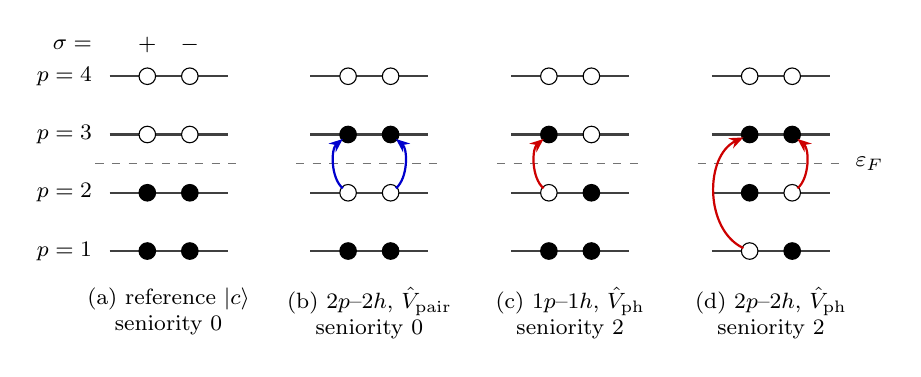
\begin{tikzpicture}[x=1cm,y=1cm,
   pairarrow/.style={-{Stealth[length=5pt,width=4pt]},thick,Blue3,
                     shorten >=2.5pt,shorten <=2.5pt},
   pharrow/.style={-{Stealth[length=5pt,width=4pt]},thick,Red3,
                   shorten >=2.5pt,shorten <=2.5pt}]

\levelpanel{A}{0cm}{1-u,1-d,2-u,2-d}%
  {(a) reference $\vert c\rangle$\\ seniority $0$}
\levelpanel{B}{2.55cm}{1-u,1-d,3-u,3-d}%
  {(b) $2p$--$2h$, $\hat{V}_{\mathrm{pair}}$\\ seniority $0$}
\levelpanel{C}{5.10cm}{1-u,1-d,2-d,3-u}%
  {(c) $1p$--$1h$, $\hat{V}_{\mathrm{ph}}$\\ seniority $2$}
\levelpanel{D}{7.65cm}{1-d,2-u,3-u,3-d}%
  {(d) $2p$--$2h$, $\hat{V}_{\mathrm{ph}}$\\ seniority $2$}

\draw[pairarrow] (B-2-u) to[bend left=50] (B-3-u);
\draw[pairarrow] (B-2-d) to[bend right=50] (B-3-d);
\draw[pharrow]   (C-2-u) to[bend left=50] (C-3-u);
\draw[pharrow]   (D-2-d) to[bend right=50] (D-3-d);
\draw[pharrow]   (D-1-u) to[out=155,in=205,looseness=1.1] (D-3-u);

\node[left,font=\footnotesize] at (-0.20,0)    {$p=1$};
\node[left,font=\footnotesize] at (-0.20,0.74) {$p=2$};
\node[left,font=\footnotesize] at (-0.20,1.48) {$p=3$};
\node[left,font=\footnotesize] at (-0.20,2.22) {$p=4$};
\node[right,font=\footnotesize] at (9.25,{0.74*1.5}) {$\varepsilon_F$};
\node[font=\footnotesize] at (0.38,2.62) {$+$};
\node[font=\footnotesize] at (0.92,2.62) {$-$};
\node[left,font=\footnotesize] at (-0.20,2.62) {$\sigma=$};
\end{tikzpicture}
\caption{Single-particle levels of the pairing model with $L=4$ doubly
degenerate levels, $\varepsilon_p=(p-1)\xi$, and $N=4$ particles.  Each level
carries two slots, $\sigma=+$ and $\sigma=-$; a filled circle is an occupied
spin-orbital and an open circle an empty one, so an open circle below
$\varepsilon_F$ is a hole.  (a) The reference determinant.  (b) A
two-particle-two-hole excitation produced by the pairing term
$\hat{V}_{\mathrm{pair}}$: a complete pair is carried from level $2$ to level
$3$ and the seniority stays zero.  (c) A one-particle-one-hole excitation and
(d) a pair-breaking two-particle-two-hole excitation, both of which require
the particle-hole term $\hat{V}_{\mathrm{ph}}$ of Eq.~(\ref{eq:4-Vph}) and
both of which have seniority two.  In the pure pairing model panels (c) and
(d) are unreachable from (a).}
\label{fig:4-levels}
\end{figure}

\paragraph{The price: the seniority-zero space is no longer closed.}
Because $\hat{V}_{\mathrm{ph}}$ breaks pairs, we can no longer work with the
six pair configurations of Section~\ref{sec:pairingmodel}.  What survives is
the weaker statement that both terms conserve $N_+$ and $N_-$ separately, so
$S_z=(N_+-N_-)/2$ is still a good quantum number.  For $L=4$ and $N=4$ the
full space has $\binom{8}{4}=70$ determinants and the balanced sector
$S_z=0$ has $36$ -- six times the seniority-zero dimension, and the price of
one extra term.

Table~\ref{tab:pairingphcoupling} makes the content of
Figure~\ref{fig:4-levels} quantitative.  It lists every determinant that the
Hamiltonian connects directly to the reference, classified by excitation rank
and seniority, together with the matrix element.  At $f=0$ there are four such
determinants and they are all of type~(b).  At $f\ne0$ two further families
appear, exactly as the figure suggests, and the seniority-zero matrix element
picks up the promised $g\to g+f$.

\begin{table}[h]
\centering
\renewcommand{\arraystretch}{1.25}
\setlength{\tabcolsep}{10pt}
\begin{tabular}{llrl}
\toprule
\textbf{Channel} & \textbf{Seniority} & \textbf{Number} &
$\bra{\Phi}\hat{H}\bket{c}$\\
\midrule
\multicolumn{4}{l}{\emph{$g=1$, $f=0$: the pairing model}}\\
$2p$--$2h$ & $0$ & $4$ & $-g/2$\\
\midrule
\multicolumn{4}{l}{\emph{$g=1$, $f=0.05$}}\\
$1p$--$1h$ & $2$ & $8$ & $\pm f/2$\\
$2p$--$2h$ & $0$ & $4$ & $-(g+f)/2$\\
$2p$--$2h$ & $2$ & $8$ & $\pm f/2$\\
\bottomrule
\end{tabular}
\caption{The determinants connected to the reference by one action of the
Hamiltonian, for $L=4$ and $N=4$ in the $S_z=0$ sector.  With $f=0$ only the
seniority-zero two-particle-two-hole states are reached, which is why the
particle-hole channel of the pairing model is empty.  Computed by
\texttt{models.py}.}
\label{tab:pairingphcoupling}
\end{table}

The effect on the ground state is shown in Table~\ref{tab:pairingph}.  The
first row is the pairing model, and reproduces the $g=1$ entry of
Table~\ref{tab:pairing} exactly -- a check worth making, since the two rows
are computed in spaces of dimension six and thirty-six respectively.  As $f$
grows the correlation energy grows much faster than the reference energy
falls, which is the signature of a second, competing mean field; the whole of
Chapter~\ref{chap:mfapplications} is about deciding which of the two to build
the fluctuations on.

\begin{table}[h]
\centering
\renewcommand{\arraystretch}{1.25}
\setlength{\tabcolsep}{12pt}
\begin{tabular}{rrlll}
\toprule
$g$ & $f$ & $E_{\mathrm{ref}}$ & $E_0$ (exact) & $E_{\mathrm{corr}}$\\
\midrule
$1.00$ & $0.00$ & $1.0000$ & $\phantom{-}0.63554847$ & $-0.36445153$\\
$1.00$ & $0.05$ & $0.9000$ & $\phantom{-}0.45058234$ & $-0.44941766$\\
$1.00$ & $0.20$ & $0.6000$ & $-0.18348455$ & $-0.78348455$\\
$1.00$ & $0.50$ & $0.0000$ & $-1.69173670$ & $-1.69173670$\\
\bottomrule
\end{tabular}
\caption{The pairing model with a particle-hole term, $L=4$, $N=4$, $\xi=1$,
diagonalised in the $36$-dimensional $S_z=0$ sector.  The first row is the
pairing model and agrees with Table~\ref{tab:pairing} to all digits shown.}
\label{tab:pairingph}
\end{table}

\begin{notebox}
\textbf{Why this model matters.} A model with one interaction tests one
approximation.  With two competing interactions and two strengths, the same
system can be driven from a regime where a pairing mean field is right to one
where a particle-hole mean field is, and one can watch each approximation fail
where it should.  That is precisely what Chapter~\ref{chap:mfapplications}
does with the Tamm-Dancoff approximation, the random-phase approximation, BCS
and the quasiparticle RPA, all measured against the exact diagonalisation of
this section.
\end{notebox}

%----------------------------------------------------------------------
\section{The Fermi-Hubbard model}
\label{sec:hubbard}

\index{Hubbard model}
The two models so far live in an abstract single-particle space with no
geometry.  The Fermi-Hubbard model introduces a lattice, and with it the
competition that dominates the physics of correlated electrons: kinetic energy
wants to delocalise the particles, the interaction wants to keep them apart.

Electrons hop between neighbouring sites of a lattice and pay an energy $U$
whenever two of them, necessarily of opposite spin, occupy the same site,
\begin{equation}
  \boxed{\;
  \hat{H} = -\sum_{\langle ij\rangle\sigma} t_{ij}
    \left(c^{\dagger}_{i\sigma}c_{j\sigma} + \mathrm{h.c.}\right)
  + U\sum_i \hat{n}_{i\uparrow}\hat{n}_{i\downarrow} \;}
  \label{eq:4-hubbardH}
\end{equation}
with $\hat{n}_{i\sigma}=c^{\dagger}_{i\sigma}c_{i\sigma}$.  This is again
Eq.~(\ref{eq:4-generalH}): the one-body part is the hopping matrix, and the
only non-vanishing two-body matrix element is the on-site one.

The single-particle basis is now the set of lattice sites, so the creation
operators carry a position label.  Fermionic antisymmetry is enforced by the
Jordan-Wigner string: $c^{\dagger}_i c_j$ acting on an occupation-number state
picks up the parity of the occupied sites strictly between $i$ and $j$, which
is exactly the phase computed by the bit-counting algorithm at the end of
Chapter~\ref{chap:secondquant}.

\paragraph{Symmetries and sector dimensions.}
The Hamiltonian conserves $N_{\uparrow}$ and $N_{\downarrow}$ separately, so
we may diagonalise in a fixed sector of dimension
\begin{equation}
  \dim = \binom{N}{N_{\uparrow}}\binom{N}{N_{\downarrow}} .
  \label{eq:4-hubbarddim}
\end{equation}
Better still, the hopping term acts on the two spin species independently, so
the sector factorises as a tensor product and the kinetic part of the
Hamiltonian is
\begin{equation}
  \bm{K}_{\uparrow}\otimes\bm{I}_{\downarrow}
  + \bm{I}_{\uparrow}\otimes\bm{K}_{\downarrow},
  \label{eq:4-hubbardkron}
\end{equation}
the tensor-product construction of Section~\ref{sec:tensor} used in earnest.
The interaction is diagonal in the occupation basis.  On a periodic chain
translational invariance gives a further reduction into momentum sectors.

\paragraph{From metal to Mott insulator.}
Table~\ref{tab:hubbard} follows the half-filled four-site ring as $U$ grows.
At $U=0$ the model is exact free fermions: the single-particle energies are
$\varepsilon_k=-2t\cos k$ with $k=0,\pm\pi/2,\pi$, and filling the two lowest
levels for each spin gives $E_0=-4t$, which the diagonalisation reproduces.
As $U$ increases, the double occupancy falls steadily -- the electrons avoid
each other -- and the ground-state energy rises towards zero.

\begin{table}[h]
\centering
\renewcommand{\arraystretch}{1.25}
\setlength{\tabcolsep}{12pt}
\begin{tabular}{rlll}
\toprule
$U/t$ & $E_0/t$ & $E_0/(Nt)$ & $\sum_i\langle n_{i\uparrow}n_{i\downarrow}\rangle$\\
\midrule
$0$  & $-4.00000000$ & $-1.000000$ & $1.000000$\\
$2$  & $-2.82842712$ & $-0.707107$ & $0.453082$\\
$4$  & $-2.10274848$ & $-0.525687$ & $0.287325$\\
$8$  & $-1.32023496$ & $-0.330059$ & $0.129992$\\
$16$ & $-0.72286432$ & $-0.180716$ & $0.042033$\\
\bottomrule
\end{tabular}
\caption{The half-filled four-site Hubbard ring, $N_{\uparrow}=N_{\downarrow}
=2$, sector dimension $36$.  The last column is the total double occupancy in
the ground state.}
\label{tab:hubbard}
\end{table}

\paragraph{The strong-coupling limit.}
When $U\gg t$ the doubly occupied states are pushed far up in energy and can
be eliminated perturbatively.  What remains is a model of localised spins,
\begin{equation}
  \hat{H}_{tJ} = \hat{P}_G\left[
    -\sum_{\langle ij\rangle\sigma}t_{ij}
      \left(c^{\dagger}_{i\sigma}c_{j\sigma}+\mathrm{h.c.}\right)
    \right]\hat{P}_G
  + \sum_{\langle ij\rangle}J_{ij}
    \left[\bm{S}_i\cdot\bm{S}_j
      - \tfrac14\hat{P}_G\hat{n}_i\hat{n}_j\hat{P}_G\right],
  \qquad J_{ij}=\frac{4t_{ij}^2}{U},
  \label{eq:4-tJ}
\end{equation}
where $\hat{P}_G$ is the Gutzwiller projector removing all doubly occupied
sites.  At half filling there is no empty site to hop into, the kinetic term
is frozen, and the $t$-$J$ model reduces to the Heisenberg antiferromagnet.

This is a prediction we can check.  For the four-site ring the Heisenberg part
contributes $-2J$ and the constant $-\tfrac14 n_i n_j$ term on four bonds
contributes $-J$, so $E_0\rightarrow-3J=-12t^2/U$.
Table~\ref{tab:hubbardstrong} shows the ratio $E_0/J$ converging to $-3$.

\begin{table}[h]
\centering
\renewcommand{\arraystretch}{1.25}
\setlength{\tabcolsep}{14pt}
\begin{tabular}{rll}
\toprule
$U/t$ & $E_0/t$ & $E_0/J$, \quad $J=4t^2/U$\\
\midrule
$8$   & $-1.3202349583$ & $-2.64047$\\
$16$  & $-0.7228643224$ & $-2.89146$\\
$32$  & $-0.3714104223$ & $-2.97128$\\
$64$  & $-0.1870445461$ & $-2.99271$\\
$128$ & $-0.0936928521$ & $-2.99817$\\
\bottomrule
\end{tabular}
\caption{The half-filled four-site Hubbard ring at strong coupling.  The ratio
converges to $-3$, confirming the mapping onto the Heisenberg model with
$J=4t^2/U$.}
\label{tab:hubbardstrong}
\end{table}

\begin{notebox}
\textbf{Why this model matters.} The Hubbard model is the minimal model of
strong correlation.  It is believed to contain the essential physics of the
cuprate superconductors, it is the standard benchmark for quantum Monte Carlo,
tensor-network and machine-learning wave functions, and it is among the first
targets for quantum simulation with cold atoms and with quantum computers.  It
is also the model in which the exponential wall of Section~\ref{sec:expdim}
bites hardest: the sector dimension~(\ref{eq:4-hubbarddim}) for a $4\times4$
lattice at half filling is already $1.66\times10^8$, and the two-dimensional
model remains unsolved.
\end{notebox}

%----------------------------------------------------------------------
\section{The Calogero-Sutherland model}
\label{sec:calogero}

\index{Calogero-Sutherland model}
The three models above are solvable because a symmetry cuts the Hilbert space
down to a manageable size.  The Calogero-Sutherland
model~\cite{calogero1971,sutherland1971} is solvable for a different and much
rarer reason: it is \emph{integrable}, and its ground state is known in closed
form for any number of particles.

The Calogero model describes $N$ particles on a line in a harmonic trap,
interacting through an inverse-square potential,
\begin{equation}
  \hat{H} = -\frac{\hbar^2}{2m}\sum_{i=1}^{N}
      \frac{\partial^2}{\partial x_i^2}
    + \frac{m\omega^2}{2}\sum_{i=1}^{N}x_i^2
    + \sum_{i<j}\frac{g}{(x_i-x_j)^2} .
  \label{eq:4-calogeroH}
\end{equation}
It is conventional to parametrise the coupling as
\begin{equation}
  g = \frac{\hbar^2}{m}\lambda(\lambda-1),
  \label{eq:4-calogerocoupling}
\end{equation}
so that $\lambda$ measures the interaction strength.  The Sutherland model is
the same system on a ring of circumference $L$, with the inverse square
replaced by the chord distance,
\begin{equation}
  \hat{H} = -\frac{\hbar^2}{2m}\sum_i\frac{\partial^2}{\partial x_i^2}
    + \frac{\hbar^2}{m}\left(\frac{\pi}{L}\right)^2\sum_{i<j}
      \frac{\lambda(\lambda-1)}{\sin^2\!\left(\pi(x_i-x_j)/L\right)} .
  \label{eq:4-sutherlandH}
\end{equation}

\paragraph{The exact ground state.}
In units $\hbar=m=1$ the ground state of Eq.~(\ref{eq:4-calogeroH}) is
\begin{equation}
  \boxed{\;
  \Psi_0(x_1,\dots,x_N)
   = \prod_{i<j}|x_i-x_j|^{\lambda}\,
     \exp\!\left(-\frac{\omega}{2}\sum_i x_i^2\right) \;}
  \label{eq:4-calogeroground}
\end{equation}
with energy
\begin{equation}
  E_0 = \omega\left[\frac{N}{2} + \frac{\lambda N(N-1)}{2}\right] .
  \label{eq:4-calogeroenergy}
\end{equation}
Exercise~\ref{ex:4-calogero} verifies this by direct substitution; the
inverse-square form of the potential is precisely what is needed for the
cross terms generated by the Laplacian to cancel.

The factor $\prod_{i<j}|x_i-x_j|^{\lambda}$ is a \emph{Jastrow factor}, and it
is the reason this model deserves a place in a book about many-body methods.
It is a correlated wave function of exactly the type that variational Monte
Carlo optimises numerically -- but here it is exact, for every $N$ and every
$\lambda$.  The model is therefore the sharpest available test of a Jastrow
ansatz: any method that cannot reproduce Eq.~(\ref{eq:4-calogeroground}) is
missing something structural.

Two limits are instructive.  At $\lambda=0$ the coupling $g$ vanishes and the
particles are free bosons in a trap, $E_0=\omega N/2$.  At $\lambda=1$ the
coupling vanishes again, but now
\begin{equation}
  \prod_{i<j}|x_i-x_j|
  \label{eq:4-vandermonde}
\end{equation}
is the absolute value of the Vandermonde determinant of
Section~\ref{sec:applications}, which is precisely the Slater determinant of
$N$ free fermions in a harmonic trap.  The Calogero model interpolates
continuously between bosons and fermions, and for non-integer $\lambda$ it
describes particles obeying \emph{fractional statistics}.

\paragraph{A numerical check.}
For $N=2$ the centre-of-mass and relative motions separate.  With
$x=x_1-x_2$ the relative Hamiltonian is
\begin{equation}
  \hat{h}_{\mathrm{rel}} = -\frac{d^2}{dx^2}
    + \frac{\omega^2}{4}x^2 + \frac{\lambda(\lambda-1)}{x^2},
  \label{eq:4-calogerorel}
\end{equation}
whose exact ground-state energy is $\omega(\lambda+\tfrac12)$.  Discretising
on a grid and diagonalising with the machinery of
Section~\ref{sec:schrodiag} reproduces this to better than $10^{-5}$ for
$\lambda$ between $1$ and $3$, as \texttt{models.py} confirms.  The
inverse-square barrier keeps the wave function away from the origin, so the
boundary condition $\Psi\rightarrow0$ as $x\rightarrow0$ is automatic for
$\lambda>0$.

\begin{notebox}
\textbf{Why this model matters.} The Calogero-Sutherland model sits at the
junction of several subjects.  Its ground state is a Laughlin-type wave
function, $\prod_{i<j}(z_i-z_j)^m e^{-\sum|z_i|^2/4}$, connecting it to the
fractional quantum Hall effect; its excitation spectrum is that of free
particles with fractional statistics; and the probability density
$|\Psi_0|^2\propto\prod_{i<j}|x_i-x_j|^{2\lambda}e^{-\omega\sum x_i^2}$ is
exactly the eigenvalue distribution of a random matrix ensemble, with
$\beta=2\lambda$ the Dyson index.  For our purposes it is above all a
benchmark with a known answer for arbitrary $N$ -- something none of the other
models in this chapter can offer.
\end{notebox}

%----------------------------------------------------------------------
\section{What the four models have in common}
\label{sec:modelssummary}

Table~\ref{tab:models} collects the four.  The pattern is worth stating
explicitly, because it is the pattern of the whole subject.

\begin{table}[h]
\centering
\renewcommand{\arraystretch}{1.3}
\setlength{\tabcolsep}{7pt}
\begin{tabular}{lllll}
\toprule
\textbf{Model} & \textbf{Single-particle space} & \textbf{Interaction} &
\textbf{Symmetry used} & \textbf{Exactly solvable}\\
\midrule
Lipkin   & two levels, degeneracy $\Omega$ & pair transfer, spin exchange
         & $SU(2)$ quasispin & yes, block by block\\
Pairing  & $L$ doubly degenerate levels & pair transfer
         & $S$, $S_z$, seniority & yes, small $L$\\
Hubbard  & lattice sites & on-site $U$
         & $N_{\uparrow}$, $N_{\downarrow}$, momentum & 1D only\\
Calogero & continuum, $N$ particles & inverse square
         & integrability & yes, any $N$\\
\bottomrule
\end{tabular}
\caption{The four models of this chapter.  Each is the general
Hamiltonian~(\ref{eq:4-generalH}) with a drastically restricted set of
two-body matrix elements, and in each case a symmetry reduces the dimension
of the problem.}
\label{tab:models}
\end{table}

In every case the route is the same.  Write the Hamiltonian in second
quantisation; identify the operators that commute with it; use them to block
diagonalise; and solve the blocks.  The first step is
Chapter~\ref{chap:secondquant}, the second is a commutator calculation of the
kind Wick's theorem makes routine, the third is the statement that a symmetry
gives a basis in which the matrix is block diagonal
(Section~\ref{sec:spectral}), and the fourth is the eigenvalue problem of
Sections~\ref{sec:householder} and~\ref{sec:lanczos}.

What separates these models from a realistic system is only the last step of
the reduction.  In a real nucleus or a real molecule the symmetries reduce the
dimension by orders of magnitude but not to five; the matrix is sparse but
enormous; and one must fall back on the approximate methods that occupy the
rest of this book.  The value of the models in this chapter is that they let
us watch those approximations succeed and fail against an answer we already
know.

%=============================================================================
\section{Exercises}
%=============================================================================

\subsection*{Exercise 1: the Lipkin model in the quasispin basis}
\label{ex:4-lipkin}
\addcontentsline{toc}{subsection}{Exercise 1: the Lipkin model}

\begin{enumerate}
  \item[a)] Show that the quasispin operators~(\ref{eq:4-quasispin}) obey the
  angular-momentum algebra~(\ref{eq:4-su2}), using only the anticommutation
  relations of Chapter~\ref{chap:secondquant}.
  \item[b)] Show that the Lipkin Hamiltonian~(\ref{eq:4-lipkinH}) can be
  rewritten as Eq.~(\ref{eq:4-lipkinquasispin}).
  \item[c)] Show that $[\hat{H},\hat{J}^2]=0$ and $[\hat{H},\hat{N}]=0$, and
  explain what this implies for the structure of the Hamiltonian matrix.
  \item[d)] Construct the five states $\bket{2,J_z}$ for four particles, and
  compute the matrix~(\ref{eq:4-lipkinmatrix1}).  Diagonalise it and compare
  with Eq.~(\ref{eq:4-lipkinground1}).
\end{enumerate}

\paragraph{Answer to a).}
Insert the definitions and use
$\{a_l,a_k\}=\{a^{\dagger}_l,a^{\dagger}_k\}=0$ and
$\{a^{\dagger}_l,a_k\}=\delta_{lk}$.  For the first commutator,
\begin{align}
  [\hat{J}_z,\hat{J}_{\pm}]
  &= \frac{1}{2}\sum_{pp'\sigma}\sigma\left(
     a_{p\sigma}^{\dagger}a_{p\sigma}a_{p'\pm}^{\dagger}a_{p'\mp}
   - a_{p'\pm}^{\dagger}a_{p'\mp}a_{p\sigma}^{\dagger}a_{p\sigma}\right).
  \label{eq:4-exa1}
\end{align}
Anticommute the operators of the second product into the order of the first.
Using $a_{p'\mp}a_{p\sigma}^{\dagger}=\delta_{pp'}\delta_{\mp\sigma}
- a_{p\sigma}^{\dagger}a_{p'\mp}$ and then
$a_{p\sigma}a_{p'\pm}^{\dagger}=\delta_{pp'}\delta_{\pm\sigma}
- a_{p'\pm}^{\dagger}a_{p\sigma}$, the four-operator terms cancel in pairs and
what survives is
\begin{equation}
  [\hat{J}_z,\hat{J}_{\pm}]
  = \frac{1}{2}\sum_{p\sigma}\sigma\left(
     \delta_{\pm\sigma}a_{p\sigma}^{\dagger}a_{p\mp}
   - \delta_{\mp\sigma}a_{p\pm}^{\dagger}a_{p\sigma}\right)
  = \pm\frac{1}{2}\sum_p\left(
     a_{p\pm}^{\dagger}a_{p\mp} + a_{p\pm}^{\dagger}a_{p\mp}\right)
  = \pm\hat{J}_{\pm},
  \label{eq:4-exa2}
\end{equation}
where the two Kronecker deltas each pick out one value of $\sigma$, and the
factor $\sigma=\pm1$ supplies the sign.  The same manipulation gives
$[\hat{J}_+,\hat{J}_-]=2\hat{J}_z$, and $[\hat{J}^2,\hat{J}_{\pm}]=
[\hat{J}^2,\hat{J}_z]=0$ then follows from the definition
$\hat{J}^2=\hat{J}_+\hat{J}_-+\hat{J}_z^2-\hat{J}_z$ exactly as for ordinary
angular momentum.

\paragraph{Answer to b).}
The one-body part is immediate: comparing
Eqs.~(\ref{eq:4-lipkinH0}) and~(\ref{eq:4-quasispin}) gives
$\hat{H}_0=\varepsilon\hat{J}_z$.

For $\hat{H}_1$, first anticommute the two annihilation operators,
$a_{p'-\sigma}a_{p-\sigma}=-a_{p-\sigma}a_{p'-\sigma}$, and then move
$a_{p-\sigma}$ past $a_{p'\sigma}^{\dagger}$ using
$a_{p-\sigma}a_{p'\sigma}^{\dagger}
=\delta_{pp'}\delta_{-\sigma\sigma}-a_{p'\sigma}^{\dagger}a_{p-\sigma}$.
Since $\delta_{-\sigma\sigma}=0$, the delta term drops out and
\begin{equation}
  \hat{H}_1 = \frac{1}{2}V\sum_{pp'\sigma}
    a_{p\sigma}^{\dagger}a_{p-\sigma}\,
    a_{p'\sigma}^{\dagger}a_{p'-\sigma} .
  \label{eq:4-exb1}
\end{equation}
The two factors are now independent sums over $p$ and $p'$.  Writing out
$\sigma=\pm$ separately,
\begin{equation}
  \hat{H}_1 = \frac{1}{2}V\left[
    \Big(\sum_p a_{p+}^{\dagger}a_{p-}\Big)
    \Big(\sum_{p'}a_{p'+}^{\dagger}a_{p'-}\Big)
  + \Big(\sum_p a_{p-}^{\dagger}a_{p+}\Big)
    \Big(\sum_{p'}a_{p'-}^{\dagger}a_{p'+}\Big)\right]
  = \frac{1}{2}V\left(\hat{J}_+^2+\hat{J}_-^2\right).
  \label{eq:4-exb2}
\end{equation}

For $\hat{H}_2$ the same two steps give
\begin{equation}
  \hat{H}_2 = \frac{1}{2}W\left(
    -\sum_{p\sigma}a_{p\sigma}^{\dagger}a_{p\sigma}
    + \sum_{pp'\sigma}a_{p\sigma}^{\dagger}a_{p-\sigma}
      a_{p'-\sigma}^{\dagger}a_{p'\sigma}\right),
  \label{eq:4-exb3}
\end{equation}
where this time $\delta_{-\sigma-\sigma}=1$ and the delta term survives as
$-\hat{N}$.  Splitting the remaining sum over $\sigma$ as before identifies it
as $\hat{J}_+\hat{J}_-+\hat{J}_-\hat{J}_+$, so
$\hat{H}_2=\tfrac12 W(-\hat{N}+\hat{J}_+\hat{J}_-+\hat{J}_-\hat{J}_+)$.
Adding the three pieces gives Eq.~(\ref{eq:4-lipkinquasispin}).

\paragraph{Answer to c).}
Written as in Eq.~(\ref{eq:4-lipkinquasispin}), $\hat{H}$ is built entirely
from $\hat{J}_z$, $\hat{J}_{\pm}$ and $\hat{N}$.  Since $\hat{J}^2$ commutes
with each of $\hat{J}_z$ and $\hat{J}_{\pm}$ by part a), and with $\hat{N}$
trivially, it commutes with $\hat{H}$.  For $\hat{N}$: the one-body term
conserves particle number, and every term of the interaction contains two
creation and two annihilation operators, so $[\hat{H},\hat{N}]=0$.

Both $J$ and $N$ are therefore good quantum numbers.  In a basis
$\bket{J,J_z}$ the Hamiltonian matrix is block diagonal, one block for each
$J$, of dimension $2J+1$.  Within a block, $\hat{J}_z$ is diagonal and
$\hat{J}_{\pm}^2$ connects $J_z$ to $J_z\pm2$, so the block splits once more
into even and odd $J_z$.  A problem of nominal dimension
$\binom{2\Omega}{N}$ has been reduced to a set of matrices of dimension at
most $N/2+1$.

\paragraph{Answer to d).}
Start from $\bket{2,-2}$, Eq.~(\ref{eq:4-lipkinlowest}), and apply
Eq.~(\ref{eq:4-ladder}).  With $J=2$ and $J_z=-2$ the factor is
$\sqrt{6-2}=2$, so
\begin{equation}
  \bket{2,-1} = \frac{1}{2}\hat{J}_+\bket{2,-2}
   = \frac{1}{2}\Big(
     a_{1+}^{\dagger}a_{2-}^{\dagger}a_{3-}^{\dagger}a_{4-}^{\dagger}
   + a_{1-}^{\dagger}a_{2+}^{\dagger}a_{3-}^{\dagger}a_{4-}^{\dagger}
   + a_{1-}^{\dagger}a_{2-}^{\dagger}a_{3+}^{\dagger}a_{4-}^{\dagger}
   + a_{1-}^{\dagger}a_{2-}^{\dagger}a_{3-}^{\dagger}a_{4+}^{\dagger}
     \Big)\bket{0},
  \label{eq:4-exd1}
\end{equation}
one term for each substate that can be flipped.  Applying $\hat{J}_+$ again
with the factor $\sqrt{6-0}=\sqrt6$ gives $\bket{2,0}$ as the normalised sum
of the six ways of flipping two of the four substates, and so on up to
$\bket{2,2}$ with all four spins up.

The matrix elements follow from Eq.~(\ref{eq:4-lipkinquasispin}).  The
diagonal is
\begin{equation}
  \bracket{2,J_z}{\hat{H}}{2,J_z}
   = \varepsilon J_z + \frac{W}{2}\Big(-N + 2\big[J(J+1)-J_z^2\big]\Big),
  \label{eq:4-exd2}
\end{equation}
since $\hat{J}_+\hat{J}_-+\hat{J}_-\hat{J}_+=2(\hat{J}^2-\hat{J}_z^2)$.  The
off-diagonal elements come from $\tfrac12 V(\hat{J}_+^2+\hat{J}_-^2)$,
\begin{equation}
  \bracket{2,J_z+2}{\hat{H}}{2,J_z}
   = \frac{V}{2}\sqrt{J(J+1)-J_z(J_z+1)}\,
     \sqrt{J(J+1)-(J_z+1)(J_z+2)} .
  \label{eq:4-exd3}
\end{equation}
With $\varepsilon=2$, $V=-1/3$, $W=-1/4$ and $N=4$ this gives
Eq.~(\ref{eq:4-lipkinmatrix1}); for instance the $(-2,0)$ element is
$\tfrac12 V\sqrt{4}\sqrt{6}=-\sqrt6/3$, and the $J_z=-1$ diagonal element is
$-2+\tfrac12(-\tfrac14)(-4+2[6-1])=-2-\tfrac34=-\tfrac{11}{4}$.
Diagonalising reproduces Eq.~(\ref{eq:4-lipkinground1}).

\subsection*{Exercise 2: the pairing model}
\label{ex:4-pairing}
\addcontentsline{toc}{subsection}{Exercise 2: the pairing model}

\begin{enumerate}
  \item[a)] Show that $\hat{H}_0$ and $\hat{V}$ of Eq.~(\ref{eq:4-pairingH})
  commute with $\hat{S}_z$ and $\hat{S}^2$ of Eq.~(\ref{eq:4-pairingspin}).
  \item[b)] Show that the Hamiltonian can be written in the pair
  form~(\ref{eq:4-pairingpairform}), and that the pair creation operators
  commute among themselves while $(\hat{P}^{+}_p)^2=0$.
  \item[c)] Construct the Hamiltonian matrix for four particles in the four
  lowest levels, with no broken pairs and $S=0$, and find its eigenvalues as a
  function of $g$.
\end{enumerate}

\paragraph{Answer to a).}
$\hat{H}_0$ is a sum of number operators $a^{\dagger}_{p\sigma}
a_{p\sigma}$, and $\hat{S}_z$ is a weighted sum of the same operators, so the
two commute term by term.  For $\hat{V}$, note that
$a^{\dagger}_{p+}a^{\dagger}_{p-}$ creates one particle with $\sigma=+1$ and
one with $\sigma=-1$, changing $S_z$ by $\tfrac12(+1)+\tfrac12(-1)=0$;
likewise $a_{q-}a_{q+}$ destroys such a pair.  Hence $[\hat{V},\hat{S}_z]=0$.

For $\hat{S}^2$ it is enough to show $[\hat{V},\hat{S}_{\pm}]=0$.  The
operator $\hat{S}_+=\sum_p a^{\dagger}_{p+}a_{p-}$ acting on a fully paired
level gives zero, because the state $\bket{p+}$ is already occupied and
$(a^{\dagger}_{p+})^2=0$; acting on an empty level it also gives zero.  Since
$\hat{V}$ maps the fully paired space into itself,
$\hat{S}_+\hat{V}$ and $\hat{V}\hat{S}_+$ both annihilate it, and the
commutator vanishes.  Both $S$ and $S_z$ are therefore good quantum numbers
and the Hamiltonian is block diagonal in them.

\paragraph{Answer to b).}
Insert the definitions~(\ref{eq:4-pairoperators}) into
Eq.~(\ref{eq:4-pairingH}):
\begin{equation}
  -\frac{1}{2}g\sum_{pq}a^{\dagger}_{p+}a^{\dagger}_{p-}a_{q-}a_{q+}
  = -\frac{1}{2}g\sum_{pq}\hat{P}^{+}_p\hat{P}^{-}_q ,
  \label{eq:4-exp1}
\end{equation}
which is Eq.~(\ref{eq:4-pairingpairform}).

For the commutator, $\hat{P}^{+}_p\hat{P}^{+}_q
= a^{\dagger}_{p+}a^{\dagger}_{p-}a^{\dagger}_{q+}a^{\dagger}_{q-}$.  Moving
$a^{\dagger}_{q+}a^{\dagger}_{q-}$ to the front requires four interchanges of
neighbouring creation operators, each contributing a minus sign, so the total
sign is $(-1)^4=+1$ and $[\hat{P}^{+}_p,\hat{P}^{+}_q]=0$.  The pair operators
therefore behave like bosons under exchange.

They are not bosons, however.  Since
$(a^{\dagger}_{p+})^2=0$ by the Pauli principle,
\begin{equation}
  \left(\hat{P}^{+}_p\right)^2
   = a^{\dagger}_{p+}a^{\dagger}_{p-}a^{\dagger}_{p+}a^{\dagger}_{p-}
   = -\left(a^{\dagger}_{p+}\right)^2
      \left(a^{\dagger}_{p-}\right)^2 = 0 .
  \label{eq:4-exp2}
\end{equation}
A level can hold one pair but not two.  This is the hard-core constraint that
distinguishes the pairing model from a gas of free bosons, and it is what
makes the model non-trivial.

\paragraph{Answer to c).}
With four levels and two pairs there are $\binom{4}{2}=6$ basis states, which
we label by the occupied levels: $(12)$, $(13)$, $(14)$, $(23)$, $(24)$,
$(34)$.  The diagonal element of a configuration is
$2\sum_{p\in\mathrm{occ}}(p-1) - g$, the last term coming from the $p=q$ terms
of the interaction with two pairs present.  Every pair of configurations
differing by the position of one pair is connected by $-g/2$; configurations
differing in both pairs are not connected.  Ordering the basis as above,
\begin{equation}
  \bm{H} =
  \begin{bmatrix}
    2-g & -g/2 & -g/2 & -g/2 & -g/2 & 0\\
    -g/2 & 4-g & -g/2 & -g/2 & 0 & -g/2\\
    -g/2 & -g/2 & 6-g & 0 & -g/2 & -g/2\\
    -g/2 & -g/2 & 0 & 6-g & -g/2 & -g/2\\
    -g/2 & 0 & -g/2 & -g/2 & 8-g & -g/2\\
    0 & -g/2 & -g/2 & -g/2 & -g/2 & 10-g
  \end{bmatrix}.
  \label{eq:4-exp3}
\end{equation}
Diagonalising for a range of $g$ gives Table~\ref{tab:pairing}.  Note that the
$(13)$ and $(23)$ configurations are degenerate at $g=0$ -- both have
unperturbed energy $6$ -- and that the correlation energy is negative for both
signs of $g$, since the interaction can always lower the energy by mixing
configurations.

\subsection*{Exercise 3: the Hubbard model}
\label{ex:4-hubbard}
\addcontentsline{toc}{subsection}{Exercise 3: the Hubbard model}

\begin{enumerate}
  \item[a)] Show that the Hubbard Hamiltonian~(\ref{eq:4-hubbardH}) conserves
  $N_{\uparrow}$ and $N_{\downarrow}$ separately, and hence $S_z$.
  \item[b)] Diagonalise the $U=0$ Hubbard ring analytically and verify the
  entry $E_0=-4t$ of Table~\ref{tab:hubbard}.
  \item[c)] Derive the effective spin Hamiltonian in the limit $U\gg t$ at
  half filling, and predict the ratio $E_0/J$ for the four-site ring.
\end{enumerate}

\paragraph{Answer to a).}
The hopping term contains $c^{\dagger}_{i\sigma}c_{j\sigma}$ with the
\emph{same} $\sigma$ on both operators, so it conserves the number of
particles of each spin separately.  The interaction is a product of number
operators and conserves everything.  Hence $[\hat{H},\hat{N}_{\uparrow}]
=[\hat{H},\hat{N}_{\downarrow}]=0$, and since
$\hat{S}_z=\tfrac12(\hat{N}_{\uparrow}-\hat{N}_{\downarrow})$, also
$[\hat{H},\hat{S}_z]=0$.  This is what allows the diagonalisation to be
carried out in a fixed sector of dimension~(\ref{eq:4-hubbarddim}).

\paragraph{Answer to b).}
At $U=0$ the Hamiltonian is a sum of independent one-body problems.  On a ring
of $N$ sites with periodic boundary conditions the hopping matrix is
diagonalised by plane waves $c^{\dagger}_{k\sigma}=N^{-1/2}\sum_j
e^{\imath k j}c^{\dagger}_{j\sigma}$ with $k=2\pi n/N$, giving
\begin{equation}
  \varepsilon_k = -2t\cos k .
  \label{eq:4-exh1}
\end{equation}
For $N=4$ the allowed momenta are $k=0,\pm\pi/2,\pi$ with energies
$-2t$, $0$, $0$, $+2t$.  Filling the two lowest for each spin gives
$-2t+0=-2t$ per spin species, hence $E_0=-4t$, which is the first line of
Table~\ref{tab:hubbard}.  The degeneracy at $k=\pm\pi/2$ means the $U=0$
ground state is not unique; switching on $U$ lifts the degeneracy.

\paragraph{Answer to c).}
At half filling and $U\gg t$ every site carries exactly one electron in the
ground state, and states with a doubly occupied site lie an energy $U$ higher.
Treat the hopping as a perturbation.  A single hop creates a doubly occupied
site and an empty one, costing $U$; hopping back restores a singly occupied
configuration.  Second-order perturbation theory therefore gives an energy
gain $-2t^2/U$ for each such virtual excursion, and the process is possible
only if the two spins involved are antiparallel, since the Pauli principle
forbids two electrons of the same spin on one site.

Collecting the terms gives the Heisenberg Hamiltonian
\begin{equation}
  \hat{H}_{\mathrm{eff}}
   = J\sum_{\langle ij\rangle}\left(\bm{S}_i\cdot\bm{S}_j
     - \frac{\hat{n}_i\hat{n}_j}{4}\right),
  \qquad J = \frac{4t^2}{U},
  \label{eq:4-exh2}
\end{equation}
which is the half-filled limit of the $t$-$J$ model, Eq.~(\ref{eq:4-tJ}).
For the four-site ring the Heisenberg ground-state energy is $-2J$, and the
constant $-\tfrac14 n_i n_j$ contributes $-\tfrac14$ per bond on four bonds,
that is $-J$.  Hence
\begin{equation}
  E_0 \longrightarrow -3J = -\frac{12t^2}{U},
  \qquad\text{so}\qquad \frac{E_0}{J}\longrightarrow-3,
  \label{eq:4-exh3}
\end{equation}
which is what Table~\ref{tab:hubbardstrong} confirms numerically.

\subsection*{Exercise 4: the Calogero ground state}
\label{ex:4-calogero}
\addcontentsline{toc}{subsection}{Exercise 4: the Calogero ground state}

\begin{enumerate}
  \item[a)] Verify by direct substitution that
  Eq.~(\ref{eq:4-calogeroground}) is an eigenstate of
  Eq.~(\ref{eq:4-calogeroH}) with energy~(\ref{eq:4-calogeroenergy}).
  \item[b)] Show that at $\lambda=1$ the ground state is the Slater
  determinant of $N$ free fermions in a harmonic trap.
  \item[c)] Separate the $N=2$ problem and verify the relative energy
  $\omega(\lambda+\tfrac12)$.
\end{enumerate}

\paragraph{Answer to a).}
Work in units $\hbar=m=1$ and write $\Psi_0=e^{-\Phi}$ with
\begin{equation}
  \Phi = \frac{\omega}{2}\sum_i x_i^2
       - \lambda\sum_{i<j}\ln|x_i-x_j| .
  \label{eq:4-exc1}
\end{equation}
For any such form,
\begin{equation}
  -\frac{1}{2}\sum_i\frac{\partial^2\Psi_0}{\partial x_i^2}
   = \frac{1}{2}\left[\sum_i\frac{\partial^2\Phi}{\partial x_i^2}
     - \sum_i\left(\frac{\partial\Phi}{\partial x_i}\right)^2\right]\Psi_0 .
  \label{eq:4-exc2}
\end{equation}
The derivatives are
\begin{equation}
  \frac{\partial\Phi}{\partial x_i} = \omega x_i
    - \lambda\sum_{j\ne i}\frac{1}{x_i-x_j},
  \qquad
  \frac{\partial^2\Phi}{\partial x_i^2} = \omega
    + \lambda\sum_{j\ne i}\frac{1}{(x_i-x_j)^2} .
  \label{eq:4-exc3}
\end{equation}
Squaring the first,
\begin{equation}
  \sum_i\left(\frac{\partial\Phi}{\partial x_i}\right)^2
   = \omega^2\sum_i x_i^2
   - 2\lambda\omega\sum_i\sum_{j\ne i}\frac{x_i}{x_i-x_j}
   + \lambda^2\sum_i\sum_{j\ne i}\sum_{k\ne i}
     \frac{1}{(x_i-x_j)(x_i-x_k)} .
  \label{eq:4-exc4}
\end{equation}
Two simplifications now do all the work.  In the second term, pairing $(i,j)$
with $(j,i)$ gives
$x_i/(x_i-x_j)+x_j/(x_j-x_i)=1$, so the double sum equals $N(N-1)/2$ times
two, that is $-2\lambda\omega\cdot N(N-1)/2$.  In the third term the pieces
with $j=k$ give $\lambda^2\sum_{i\ne j}(x_i-x_j)^{-2}$, while the pieces with
$j\ne k$ cancel identically by the three-term identity
\begin{equation}
  \frac{1}{(x_i-x_j)(x_i-x_k)}
  + \frac{1}{(x_j-x_i)(x_j-x_k)}
  + \frac{1}{(x_k-x_i)(x_k-x_j)} = 0 .
  \label{eq:4-exc5}
\end{equation}
Assembling everything, the inverse-square terms combine as
\begin{equation}
  \frac{1}{2}\left[\lambda\sum_{i\ne j}\frac{1}{(x_i-x_j)^2}
   - \lambda^2\sum_{i\ne j}\frac{1}{(x_i-x_j)^2}\right]
   = -\lambda(\lambda-1)\sum_{i<j}\frac{1}{(x_i-x_j)^2},
  \label{eq:4-exc6}
\end{equation}
which cancels the interaction term of the Hamiltonian exactly; the
$\omega^2 x_i^2$ terms cancel the trap; and what is left is the constant
\begin{equation}
  E_0 = \frac{1}{2}\left[N\omega + \lambda\omega N(N-1)\right]
      = \omega\left[\frac{N}{2}+\frac{\lambda N(N-1)}{2}\right],
  \label{eq:4-exc7}
\end{equation}
which is Eq.~(\ref{eq:4-calogeroenergy}).  The cancellation in
Eq.~(\ref{eq:4-exc6}) works only because the interaction falls off as the
inverse \emph{square}; this is the sense in which the model is fine-tuned to
be solvable.

\paragraph{Answer to b).}
At $\lambda=1$ the coupling $g=\lambda(\lambda-1)$ vanishes and the particles
are free, but the wave function
\begin{equation}
  \Psi_0 = \prod_{i<j}|x_i-x_j|\,e^{-\omega\sum_i x_i^2/2}
  \label{eq:4-exc8}
\end{equation}
is not the bosonic ground state.  Up to an overall sign it is the Vandermonde
determinant of Section~\ref{sec:applications},
\begin{equation}
  \prod_{i<j}(x_j-x_i) = \det\left[x_i^{\,j-1}\right],
  \label{eq:4-exc9}
\end{equation}
and multiplying each column by the Gaussian and taking suitable linear
combinations turns $x_i^{j-1}e^{-\omega x_i^2/2}$ into the Hermite functions
of Section~\ref{sec:schrodiag}.  The result is precisely the Slater
determinant of the $N$ lowest harmonic oscillator orbitals.  The energy check
is immediate: Eq.~(\ref{eq:4-calogeroenergy}) with $\lambda=1$ gives
$E_0=\omega N^2/2 = \omega\sum_{n=0}^{N-1}(n+\tfrac12)$, the sum of the $N$
lowest oscillator energies.

For non-integer $\lambda$ the wave function is neither symmetric nor
antisymmetric, and the particles obey fractional statistics interpolating
between the two.

\paragraph{Answer to c).}
Introduce $X=(x_1+x_2)/2$ and $x=x_1-x_2$.  The kinetic energy separates as
$-\tfrac14\partial_X^2-\partial_x^2$ and the trap as
$\omega^2 X^2 + \tfrac14\omega^2 x^2$, so with $\hbar=m=1$
\begin{equation}
  \hat{H} = \left[-\frac{1}{4}\frac{\partial^2}{\partial X^2}
     + \omega^2 X^2\right]
   + \left[-\frac{\partial^2}{\partial x^2}
     + \frac{\omega^2}{4}x^2
     + \frac{\lambda(\lambda-1)}{x^2}\right].
  \label{eq:4-exc10}
\end{equation}
The centre-of-mass part is a harmonic oscillator with ground-state energy
$\omega/2$.  The relative part is Eq.~(\ref{eq:4-calogerorel}); its ground
state is $x^{\lambda}e^{-\omega x^2/4}$ with energy $\omega(\lambda+\tfrac12)$,
as substitution confirms.  The total is
$\omega/2+\omega(\lambda+\tfrac12)=\omega(1+\lambda)$, which agrees with
Eq.~(\ref{eq:4-calogeroenergy}) for $N=2$.  Solving the relative problem
numerically on a grid, as in Section~\ref{sec:schrodiag}, reproduces
$\omega(\lambda+\tfrac12)$ to better than $10^{-5}$; see \texttt{models.py}.

\subsection*{Exercise 5: numerical explorations}
\addcontentsline{toc}{subsection}{Exercise 5: numerical explorations}

\begin{enumerate}
  \item[a)] Using \texttt{models.py}, plot the Lipkin ground-state energy and
  the weight of $\bket{2,-2}$ in the ground state as functions of $V$ at fixed
  $\varepsilon$ and $W$.  At roughly what value of $V/\varepsilon$ does the
  single-configuration picture break down?
  \item[b)] Repeat the pairing calculation of Table~\ref{tab:pairing} for six
  and eight levels.  How does the correlation energy at $g=1$ scale with the
  number of levels?
  \item[c)] Compute the double occupancy of the Hubbard ring as a function of
  $U/t$ and identify the crossover.  Compare a six-site ring with the
  four-site one.
  \item[d)] For the pairing model with twelve levels and six pairs, compare
  the exact ground-state energy from full diagonalisation with the Lanczos
  result of Table~\ref{tab:lanczos}, and with the Schmidt truncation of
  Table~\ref{tab:schmidt}.  How many Schmidt states are needed for the energy
  to be correct to six digits?
\end{enumerate}

\part{Wave function based methods}
\clearemptydoublepage
\chapter{Full configuration interaction theory}
\label{chap:fci}

We will start our discussions of many-body methods with what is called
full configuration interaction theory, or just FCI.  The reason for
this is simple. If the effective degrees of freedom which are relevant
for describing a physical system give a sufficiently good reproduction
of the static properties (and later we will add dynamical properties)
of a many-body system, FCI gives us all relevant eigenpairs
(eigenvalues and eigenstates) and allows us to compute other
expectation values than the energy levels.

Although it would have been natural to start with mean-field methods
(FCI is often labelled as a post Hartree-Fock method), we have chosen
a slightly different route. The reason for this is that FCI,
within a restricted effective space, provides us with the exact
eigenvalues and can thus serve as a benchmark for the approximative
methods discussed in the coming chapters, from mean field methods to
the Tamm-Dancoff (TDA) and random-phase (RPA) approximations, variants of many-body
perturbation theory and coupled-cluster theory, Greens' function
approaches and other. We will use FCI to illustrate how these other
methods can be interpreeted in terms of specific truncations/approximations of
FCI.

We start thus with, what this authour likes to claim as the simplest
possible approach to many-body problems, an approach which involves us
being able to set up a many-body Hamiltonian matrix (within an
effective and reduced Hilbert space), and then simply diagonalize. The
overarching principles and the underlying mathematics are
straightforward, although the actual implementations may easily lead
to endless frustrations and sleepless nights. Let us get started.

%----------------------------------------------------------------------
\section{Slater determinants as a basis}
\label{sec:cibasis}

\index{configuration interaction}
The simplest many-body wave function is a product,
\begin{equation}
  \Psi(x_1,x_2,\dots,x_N) \approx
    \phi_1(x_1)\phi_2(x_2)\cdots\phi_N(x_N),
  \label{eq:5-product}
\end{equation}
because we are really only good at thinking about one particle at a time.
Product functions are easy to work with: if the single-particle states are
orthonormal the products are too, and matrix elements factorise into
one-dimensional integrals.  The price is the complete absence of correlations,
which must then be built up by superposing many, many products.  This is the
trade-off that runs through the whole subject -- a compact representation with
difficult integrals, or easy integrals and very many states.

Antisymmetry turns the product into a determinant, and
Chapter~\ref{chap:mbphys} showed that the two elementary properties of
determinants -- a sign change under the interchange of two columns, and
vanishing when two rows coincide -- are exactly the Pauli principle:
\begin{itemize}
  \item no two particles at the same place (two equal columns);
  \item no two particles in the same state (two equal rows).
\end{itemize}
Beyond $N=4$ the coordinate-space determinant becomes unwieldy, which is why
Chapter~\ref{chap:secondquant} replaced it by the occupation representation.
There a Slater determinant is a string of creation operators acting on the
vacuum, each index appearing at most once because
$a^{\dagger}_i a^{\dagger}_i=0$, and antisymmetry is carried by the algebra
rather than by the notation.

We take that formalism as given.  Writing the reference determinant as
\begin{equation}
  \bket{\Phi_0} = \left(\prod_{i\le F}\hat{a}_i^{\dagger}\right)\bket{0},
  \label{eq:5-reference}
\end{equation}
the excited determinants are
\begin{equation}
  \bket{\Phi_i^a} = \hat{a}_a^{\dagger}\hat{a}_i\bket{\Phi_0},
  \qquad
  \bket{\Phi_{ij}^{ab}} =
    \hat{a}_a^{\dagger}\hat{a}_b^{\dagger}\hat{a}_j\hat{a}_i\bket{\Phi_0},
  \label{eq:5-excitations}
\end{equation}
and in general
\begin{equation}
  \bket{\Phi_{ijk\dots}^{abc\dots}} =
    \hat{a}_a^{\dagger}\hat{a}_b^{\dagger}\hat{a}_c^{\dagger}\cdots
    \hat{a}_k\hat{a}_j\hat{a}_i\bket{\Phi_0},
  \label{eq:5-npnh}
\end{equation}
with the hole indices $i,j,k$ below the Fermi level and the particle indices
$a,b,c$ above it, following the convention of
Section~\ref{sec:particlehole}.  We call such a determinant an $np$-$nh$
excitation, or a \emph{configuration}.

%----------------------------------------------------------------------
\section{The configuration-interaction expansion}
\label{sec:ciexpansion}

The exact ground state is an arbitrary superposition of all of these,
\begin{equation}
  \bket{\Psi_0} = C_0\bket{\Phi_0}
    + \sum_{ai}C_i^a\bket{\Phi_i^a}
    + \sum_{abij}C_{ij}^{ab}\bket{\Phi_{ij}^{ab}} + \cdots
    = \left(C_0+\hat{C}\right)\bket{\Phi_0},
  \label{eq:5-ciexpansion}
\end{equation}
where we have introduced the \emph{correlation operator}
\begin{equation}
  \hat{C} = \sum_{ai}C_i^a\hat{a}_a^{\dagger}\hat{a}_i
    + \sum_{abij}C_{ij}^{ab}
      \hat{a}_a^{\dagger}\hat{a}_b^{\dagger}\hat{a}_j\hat{a}_i + \cdots
  \label{eq:5-correlationoperator}
\end{equation}
The normalisation of $\bket{\Psi_0}$ is at our disposal, and $C_0$ is by
hypothesis non-zero, so we may set $C_0=1$ with proportional changes in all
the other coefficients.  With this \emph{intermediate normalisation},
\begin{equation}
  \braket{\Psi_0}{\Phi_0} = \braket{\Phi_0}{\Phi_0} = 1,
  \qquad
  \bket{\Psi_0} = \left(1+\hat{C}\right)\bket{\Phi_0}.
  \label{eq:5-intermediate}
\end{equation}

It is convenient to compress the notation.  Writing $H$ for a set of
$0,1,\dots,n$ hole indices and $P$ for a set of $0,1,\dots,n$ particle
indices,
\begin{equation}
  \bket{\Psi_0} = \sum_{PH}C_H^P\bket{\Phi_H^P}
    = \left(\sum_{PH}C_H^P\hat{A}_H^P\right)\bket{\Phi_0},
  \label{eq:5-compact}
\end{equation}
with $\hat{A}_H^P$ the operator that creates the corresponding excitation.
Unit normalisation reads $\sum_{PH}|C_H^P|^2=1$, and the energy is
\begin{equation}
  E = \bracket{\Psi_0}{\hat{H}}{\Psi_0}
    = \sum_{PP'HH'}C_H^{*P}
      \bracket{\Phi_H^P}{\hat{H}}{\Phi_{H'}^{P'}}C_{H'}^{P'} .
  \label{eq:5-energy}
\end{equation}

If the expansion runs over \emph{all} determinants that can be built from the
chosen single-particle basis, this is \emph{full configuration interaction}.
The only approximation left is the truncation of the single-particle space
itself.

%----------------------------------------------------------------------
\section{The eigenvalue problem}
\label{sec:cieigenvalue}

Equation~(\ref{eq:5-energy}) is solved by diagonalisation, and it is worth
seeing why the diagonalisation is not merely convenient but is the
variational answer.  We minimise the energy subject to normalisation,
\begin{equation}
  \delta\left[\bracket{\Psi_0}{\hat{H}}{\Psi_0}
    - \lambda\braket{\Psi_0}{\Psi_0}\right] = 0,
  \label{eq:5-variation}
\end{equation}
with $\lambda$ a Lagrange multiplier.  Carrying out the variation,
\begin{equation}
  \sum_{P'H'}\Big\{\delta[C_H^{*P}]
    \bracket{\Phi_H^P}{\hat{H}}{\Phi_{H'}^{P'}}C_{H'}^{P'}
  + C_H^{*P}\bracket{\Phi_H^P}{\hat{H}}{\Phi_{H'}^{P'}}\delta[C_{H'}^{P'}]
  - \lambda\big(\delta[C_H^{*P}]C_{H'}^{P'}
    + C_H^{*P}\delta[C_{H'}^{P'}]\big)\Big\} = 0 .
  \label{eq:5-variation2}
\end{equation}
Since $\delta[C_H^{*P}]$ and $\delta[C_{H'}^{P'}]$ are complex conjugates, it
is necessary and sufficient that the quantities multiplying
$\delta[C_H^{*P}]$ vanish, giving
\begin{equation}
  \sum_{P'H'}\bracket{\Phi_H^P}{\hat{H}}{\Phi_{H'}^{P'}}C_{H'}^{P'}
    = \lambda\,C_H^{P}
  \label{eq:5-eigen}
\end{equation}
for every set $PH$.  Multiplying by $C_H^{*P}$ and summing identifies
$\lambda=E$, so the multiplier is the energy and
\begin{equation}
  \boxed{\;
  \sum_{P'H'}\bracket{\Phi_H^P}{\hat{H}-E}{\Phi_{H'}^{P'}}C_{H'}^{P'} = 0
  \;}
  \label{eq:fullci}
\end{equation}
This is the full CI equation.  The same result follows more directly by
writing $(\hat{H}-E)\bket{\Psi_0}=0$ and projecting successively onto every
$\bbra{\Phi_H^P}$.

Equation~(\ref{eq:fullci}) is a Hermitian eigenvalue problem, and the
diagonalisation is a Rayleigh-Ritz variational calculation in the space
spanned by the chosen determinants: the lowest eigenvalue is the best upper
bound to $E_0$ obtainable in that space, and it can only improve as the space
grows.  This is exactly the property that made the Lanczos algorithm of
Section~\ref{sec:lanczos} so well suited to the problem -- the lowest Ritz
value there is the same variational bound, computed in a Krylov space instead
of a space of determinants.

Everything now depends on being able to build and diagonalise the matrix
$\bracket{\Phi_H^P}{\hat{H}}{\Phi_{H'}^{P'}}$.  The matrix elements are
supplied by the Condon-Slater rules of Section~\ref{sec:wickapps}, and the
diagonalisation by the algorithms of Chapter~\ref{chap:linalg}: Householder
and QL for small matrices, Lanczos for large ones.

%----------------------------------------------------------------------
\section{The structure of the Hamiltonian matrix}
\label{sec:cimatrix}

Suppose we have six fermions below the Fermi level, so that at most
$6p$-$6h$ excitations are possible.  Ordering the determinants by excitation
level, the Hamiltonian matrix has the block structure
\begin{equation}
  \begin{array}{c|ccccccc}
     & 0p0h & 1p1h & 2p2h & 3p3h & 4p4h & 5p5h & 6p6h\\
    \hline
    0p0h & \times & \times & \times & 0 & 0 & 0 & 0\\
    1p1h & \times & \times & \times & \times & 0 & 0 & 0\\
    2p2h & \times & \times & \times & \times & \times & 0 & 0\\
    3p3h & 0 & \times & \times & \times & \times & \times & 0\\
    4p4h & 0 & 0 & \times & \times & \times & \times & \times\\
    5p5h & 0 & 0 & 0 & \times & \times & \times & \times\\
    6p6h & 0 & 0 & 0 & 0 & \times & \times & \times
  \end{array}
  \label{eq:5-blockstructure}
\end{equation}
The zeros are not accidental.  A two-body operator connects Slater
determinants differing by at most two single-particle states, which is the
last of the Condon-Slater rules of Section~\ref{sec:wickapps}.  The matrix is
therefore \emph{banded} in the excitation level, with bandwidth two, and
overwhelmingly sparse: for six particles the fraction of non-zero blocks is
already small, and it falls as the space grows.  Chapter~\ref{chap:linalg}
called this the structure that Lanczos exploits; here we see where it comes
from.

\paragraph{In a Hartree-Fock basis.}
If the single-particle states are the solutions of the Hartree-Fock equations
rather than the eigenstates of $\hat{h}_0$, one more set of elements
vanishes.  Brillouin's theorem, met in Section~\ref{sec:wickapps}, states that
\begin{equation}
  \bracket{\Phi_0}{\hat{H}}{\Phi_i^a} = 0,
  \label{eq:5-brillouin}
\end{equation}
so the reference determinant does not couple to the singles at all,
\begin{equation}
  \begin{array}{c|ccccccc}
     & 0p0h & 1p1h & 2p2h & 3p3h & 4p4h & 5p5h & 6p6h\\
    \hline
    0p0h & \tilde{\times} & 0 & \tilde{\times} & 0 & 0 & 0 & 0\\
    1p1h & 0 & \tilde{\times} & \tilde{\times} & \tilde{\times} & 0 & 0 & 0\\
    2p2h & \tilde{\times} & \tilde{\times} & \tilde{\times} & \tilde{\times}
         & \tilde{\times} & 0 & 0\\
    3p3h & 0 & \tilde{\times} & \tilde{\times} & \tilde{\times}
         & \tilde{\times} & \tilde{\times} & 0\\
    4p4h & 0 & 0 & \tilde{\times} & \tilde{\times} & \tilde{\times}
         & \tilde{\times} & \tilde{\times}\\
    5p5h & 0 & 0 & 0 & \tilde{\times} & \tilde{\times} & \tilde{\times}
         & \tilde{\times}\\
    6p6h & 0 & 0 & 0 & 0 & \tilde{\times} & \tilde{\times} & \tilde{\times}
  \end{array}
  \label{eq:5-blockstructureHF}
\end{equation}
where the tildes are a reminder that a unitary transformation of the
single-particle basis has changed every matrix element.  The correlation
energy is then carried entirely by the doubles at leading order, which is the
starting point for both many-body perturbation theory and coupled-cluster
theory.

The programme \texttt{fci.py} builds this structure explicitly.  For the
pairing model with four levels and four particles the full space has
$\binom{8}{4}=70$ determinants, distributed as $1$, $16$, $36$, $16$, $1$ over
the excitation levels $0$ to $4$, and the computed block table is
\begin{equation}
  \begin{array}{c|ccccc}
     & 0p0h & 1p1h & 2p2h & 3p3h & 4p4h\\
    \hline
    0p0h & \times & 0 & \times & 0 & 0\\
    1p1h & 0 & \times & 0 & \times & 0\\
    2p2h & \times & 0 & \times & 0 & \times\\
    3p3h & 0 & \times & 0 & \times & 0\\
    4p4h & 0 & 0 & \times & 0 & \times
  \end{array}
  \label{eq:5-pairingblocks}
\end{equation}
Even the odd blocks are empty here, because the pairing interaction moves
particles two at a time and can never change the number of broken pairs.  The
symmetry has done more work than Brillouin's theorem would.

%----------------------------------------------------------------------
\section{The exponential wall}
\label{sec:exponentialwall}

\index{exponential wall}\index{Hilbert space!dimension}
Full configuration interaction is exact, and that is precisely its problem.
With $N$ particles distributed over $n$ single-particle states the number of
Slater determinants is
\begin{equation}
  \dim\mathcal{H} = \binom{n}{N},
  \label{eq:5-dimension}
\end{equation}
which is the count of bit patterns with $N$ bits set out of $n$, in the
representation of Section~\ref{sec:bitrep}.  This is a combinatorial
expression, but combinatorial growth turns into exponential growth as soon as
the particle number scales with the size of the basis.  At half filling,
$N=n/2$, Stirling's formula gives
\begin{equation}
  \binom{n}{n/2} \sim \frac{2^{n}}{\sqrt{\pi n/2}} \sim \frac{2^{n}}{\sqrt{n}},
  \label{eq:5-stirling}
\end{equation}
so the dimension doubles every time one single-particle state is added.  The
program \texttt{fci.py} tabulates both sides:
\begin{center}
\renewcommand{\arraystretch}{1.15}
\begin{tabular}{rll}
\toprule
$n$ & $\binom{n}{n/2}$ & $2^{n}/\sqrt{n}$\\
\midrule
$10$  & $2.520\times10^{2}$  & $3.238\times10^{2}$\\
$20$  & $1.848\times10^{5}$  & $2.345\times10^{5}$\\
$40$  & $1.378\times10^{11}$ & $1.738\times10^{11}$\\
$80$  & $1.075\times10^{23}$ & $1.352\times10^{23}$\\
$160$ & $9.205\times10^{46}$ & $1.155\times10^{47}$\\
\bottomrule
\end{tabular}
\end{center}
The estimate is accurate to within a factor of order one over five decades of
$n$ and twenty-five orders of magnitude of dimension.

\paragraph{A realistic example.}
Consider oxygen-16 and let the neutrons occupy the four lowest major
oscillator shells, the $0s$, $0p$, $1s0d$ and $1p0f$ shells, which together
hold $2+6+12+20=40$ single-particle states for each species.  The eight
neutrons can be distributed in
\begin{equation}
  \binom{40}{8} = 7.690\times10^{7}
  \label{eq:5-oxygen}
\end{equation}
ways, and since the protons can be distributed independently the full
proton-neutron space has
\begin{equation}
  \binom{40}{8}^2 = 5.914\times10^{15}
  \label{eq:5-oxygen2}
\end{equation}
Slater determinants.  Rotational and parity symmetry reduce this by orders of
magnitude, but adding a single further major shell, or relaxing the
truncation, restores the growth immediately.  Direct diagonalisation by
Householder and QL, Sections~\ref{sec:householder}
and~\ref{sec:qlalgorithm}, is limited to matrices of dimension around $10^5$
because it stores and modifies the whole matrix.  Lanczos,
Section~\ref{sec:lanczos}, needs only the product $\bm{H}\bm{v}$ and reaches
perhaps $10^{10}$ on a large machine.  Beyond that no rearrangement of the
linear algebra helps: the expansion itself must be truncated.

\paragraph{The same wall in the models of Chapter~\ref{chap:systems}.}
Each of the models of the previous chapter meets Eq.~(\ref{eq:5-stirling}) in
its own way.
\begin{itemize}
  \item The \emph{Lipkin model} with $N$ particles in two $N$-fold degenerate
    levels has $\binom{2N}{N}$ determinants in total and $\binom{N}{N/2}\sim
    2^{N}/\sqrt{N}$ in the maximal-quasispin multiplet.  That the SU(2)
    structure of Section~\ref{sec:lipkin} collapses the problem to an
    $(N+1)$-dimensional matrix is a symmetry accident, not a general escape.
  \item The \emph{pairing model} of Section~\ref{sec:pairingmodel} has
    $\binom{2n}{N}$ determinants for $n$ doubly degenerate levels, of which
    only $\binom{n}{N/2}$ have seniority zero.  Again a symmetry -- here the
    conservation of the number of broken pairs -- takes the square root of
    the dimension, and again it is special to the model.
  \item The \emph{Hubbard model} of Section~\ref{sec:hubbard} has a local
    Hilbert space of dimension four, so $L$ sites give $4^{L}$ states in
    total.  At fixed particle number this becomes
    $\binom{L}{N_{\uparrow}}\binom{L}{N_{\downarrow}}$,
    Eq.~(\ref{eq:4-hubbarddim}), which is again exponential at any extensive
    filling.
  \item A \emph{spin chain}, the limit of the Hubbard model at large $U$, has
    no combinatorial disguise at all:
    $\mathcal{H}=\bigotimes_{i=1}^{L}\mathbb{C}^2$ has dimension $2^{L}$ by
    construction.
\end{itemize}
The pattern is worth stating plainly.  Combinatorial counting and
tensor-product structure are two faces of the same growth; the tensor product
is fundamental, the binomial coefficient is what survives after a conservation
law has been imposed.  A conserved quantity can remove a factor, but never the
exponential.

\begin{notebox}
\textbf{Why the wall is not the end of the story.}  The dimension of
$\mathcal{H}$ counts the coefficients an \emph{arbitrary} state would need.
Physical ground states are not arbitrary.  For local Hamiltonians with a gap,
the entanglement entropy across a cut grows with the area of the cut rather
than with the volume it encloses, and states obeying such an area law are
described to high accuracy by a number of parameters polynomial in $L$.  The
Schmidt decomposition of Section~\ref{sec:schmidt} is the one-cut version of
this statement, and the singular values decaying rapidly is exactly what
makes the truncation work.  Applying it at every bond of a chain gives a
matrix product state,
\begin{equation}
  \bket{\psi} = \sum_{s_1\dots s_L}
    A^{s_1}_1A^{s_2}_2\cdots A^{s_L}_L\,\bket{s_1s_2\dots s_L},
  \label{eq:5-mps}
\end{equation}
whose cost is polynomial in the bond dimension $D$; this is the density-matrix
renormalisation group.  The same idea appears elsewhere in this book in
different clothing: a neural-network quantum state replaces the exponentially
many amplitudes by a polynomially parameterised function of the occupation
pattern, and quantum computing replaces them by $n$ qubits whose Hilbert space
is exponential by construction.  Full CI is the reference against which all
of these compressions are measured, which is why we treat it first.
\end{notebox}

%----------------------------------------------------------------------
\section{Full CI for the pairing model}
\label{sec:fcipairing}

The pairing Hamiltonian of Section~\ref{sec:pairingmodel},
\begin{equation}
  \hat{H} = \xi\sum_{p\sigma}(p-1)\hat{a}^{\dagger}_{p\sigma}
    \hat{a}_{p\sigma}
  - \frac{1}{2}g\sum_{pq}\hat{a}^{\dagger}_{p+}\hat{a}^{\dagger}_{p-}
    \hat{a}_{q-}\hat{a}_{q+},
  \label{eq:5-pairingH}
\end{equation}
is the ideal first test.  It is small enough to diagonalise in the full
space, and Chapter~\ref{chap:systems} already gave the exact answer in the
seniority-zero subspace, so the two calculations can be checked against each
other.

Take four doubly degenerate levels and four particles, $\xi=1$.  The full
space has $\binom{8}{4}=70$ determinants, distributed over the excitation
levels as $1$, $16$, $36$, $16$, $1$.  The seniority-zero subspace used in
Chapter~\ref{chap:systems} has only $\binom{4}{2}=6$ states.  Diagonalising
the $70\times70$ matrix at $g=1$ gives $E_0=0.63554847$, identical to the
value in Table~\ref{tab:pairing} to all digits shown.  The determinants with
broken pairs are present in the basis but carry no amplitude in the ground
state, because the interaction cannot create a broken pair from a paired
configuration.  The symmetry that we imposed by hand in Chapter~\ref{chap:systems}
is recovered automatically by the diagonalisation.

This is the general situation.  A symmetry of $\hat{H}$ block-diagonalises the
FCI matrix, and one may either exploit it, gaining a smaller matrix and a
labelled spectrum, or ignore it, gaining a simpler code at the cost of
diagonalising a larger matrix.  Production codes exploit it; the program
accompanying this chapter does not, precisely so that the two answers can be
compared.

%----------------------------------------------------------------------
\section{Full CI for the Hubbard model}
\label{sec:fcihubbard}

The Hubbard model of Section~\ref{sec:hubbard} is the harder test, and the
more instructive one.  We take a ring of $L=6$ sites at half filling,
$N_{\uparrow}=N_{\downarrow}=3$, and work in the momentum basis, where the
hopping term is diagonal,
\begin{equation}
  \hat{H} = \sum_{k\sigma}\varepsilon_k
    \hat{c}^{\dagger}_{k\sigma}\hat{c}_{k\sigma}
  + \frac{U}{L}\sum_{kk'q}
    \hat{c}^{\dagger}_{k+q\uparrow}\hat{c}^{\dagger}_{k'-q\downarrow}
    \hat{c}_{k'\downarrow}\hat{c}_{k\uparrow},
  \qquad
  \varepsilon_k = -2t\cos k,
  \label{eq:5-hubbardmom}
\end{equation}
with $k=2\pi m/L$.  In this basis the non-interacting ground state is a single
determinant -- the Fermi sea -- so the machinery of
Section~\ref{sec:ciexpansion} applies directly with $\bket{\Phi_0}$ the filled
Fermi sea.  The dimension is $\binom{6}{3}^2=400$, with the excitation levels
populated as $1$, $18$, $99$, $164$, $99$, $18$, $1$.

The interesting quantity is how much of the correlation energy survives
truncation as $U/t$ grows:
\begin{center}
\renewcommand{\arraystretch}{1.2}
\begin{tabular}{rlllll}
\toprule
$U/t$ & $E_{\mathrm{ref}}$ & CIS & CID & CISD & FCI\\
\midrule
$1$ & $-6.500000$ & $-6.50000000$ & $-6.59980159$ & $-6.59989778$ & $-6.60115829$\\
$2$ & $-5.000000$ & $-5.00000000$ & $-5.38877703$ & $-5.39026458$ & $-5.40945685$\\
$4$ & $-2.000000$ & $-2.00000000$ & $-3.41192866$ & $-3.43018837$ & $-3.66870618$\\
$8$ & $\phantom{-}4.000000$ & $\phantom{-}2.48338852$ & $-0.36779217$ & $-1.05692183$ & $-2.04813089$\\
\bottomrule
\end{tabular}
\end{center}
The doubles recover $98.66\%$ of the correlation energy at $U/t=1$ but only
$72.22\%$ at $U/t=8$.  Two features deserve comment.

First, the reference does not couple to the singles at all: the interaction
conserves total momentum, and a single excitation changes it, so
$\bracket{\Phi_0}{\hat{H}}{\Phi_i^a}=0$ exactly, for every $U$.  This is
Brillouin's theorem, Eq.~(\ref{eq:5-brillouin}), enforced here by a symmetry
rather than by a variational condition -- the plane-wave determinant is the
Hartree-Fock solution of a translationally invariant problem.  The CIS matrix
is therefore block diagonal, and its lowest eigenvalue is the smaller of the
reference energy and the lowest eigenvalue of the singles block alone.  For
$U/t\le 4$ the reference wins and CIS reproduces it exactly.  At $U/t=8$ it
does not: the singles block, strongly mixed by the large interaction, has an
eigenvalue at $2.483$, below the reference at $4.000$.  The number in the
table is that eigenvalue, and the state it belongs to is orthogonal to
$\bket{\Phi_0}$.  What CIS reports as a ground state is by then not a
correlated version of the reference at all.

Second, the deterioration with $U/t$ is the signature of \emph{strong
correlation}.  At small $U$ the ground state is a single determinant with
small corrections and any method built on that picture works.  At large $U$
the ground state is a superposition of very many determinants with comparable
weight, the reference is a poor starting point, and a truncation at any fixed
excitation level fails.  This is where the tensor-network and quantum-computing
approaches of the later chapters become attractive, and it is why the Hubbard
model at intermediate $U/t$ remains a benchmark problem.

%----------------------------------------------------------------------
\section{Truncating the expansion}
\label{sec:citruncations}

\index{configuration interaction!truncated}
Since the full expansion is out of reach for all but the smallest systems, we
truncate it.  The natural truncation is by excitation level: keep all
determinants up to $n$ particle-hole pairs and discard the rest.  This gives
the familiar hierarchy
\begin{align}
  \bket{\Psi_{\mathrm{CIS}}} &=
    \left(1+\hat{C}_1\right)\bket{\Phi_0},
  \label{eq:5-cis}\\
  \bket{\Psi_{\mathrm{CID}}} &=
    \left(1+\hat{C}_2\right)\bket{\Phi_0},
  \label{eq:5-cid}\\
  \bket{\Psi_{\mathrm{CISD}}} &=
    \left(1+\hat{C}_1+\hat{C}_2\right)\bket{\Phi_0},
  \label{eq:5-cisd}
\end{align}
and so on to CISDT, CISDTQ, until at $\hat{C}_N$ we are back at full CI.
Each of these is again a variational calculation in a subspace, so each
lowest eigenvalue is an upper bound to $E_0$ and the bounds decrease
monotonically as the truncation is relaxed.  The cost, for a basis of $n$
states and $N$ particles, is roughly $\binom{N}{k}\binom{n-N}{k}$ determinants
at excitation level $k$, that is polynomial of degree $2k$ -- which is why
CISD, at $\mathcal{O}(n^6)$, is affordable and CISDTQ, at
$\mathcal{O}(n^{10})$, is not.

For the pairing model with four levels and four particles the truncated
spaces have dimensions $1$, $17$, $53$, $69$, $70$, and the energies are
\begin{center}
\renewcommand{\arraystretch}{1.2}
\begin{tabular}{rlllll}
\toprule
$g$ & $E_{\mathrm{ref}}$ & CIS & CID & CISD & FCI\\
\midrule
$0.25$ & $1.750000$ & $1.75000000$ & $1.73050700$ & $1.73050700$ & $1.73045985$\\
$0.50$ & $1.500000$ & $1.50000000$ & $1.41759645$ & $1.41759645$ & $1.41677428$\\
$1.00$ & $1.000000$ & $1.00000000$ & $0.64890655$ & $0.64890655$ & $0.63554847$\\
$2.00$ & $0.000000$ & $0.00000000$ & $-1.35208670$ & $-1.35208670$ & $-1.48965216$\\
\bottomrule
\end{tabular}
\end{center}
The singles change nothing at all, and CISD coincides with CID: the pairing
interaction moves pairs and cannot break them, so it has no matrix element
between the reference and a $1p$-$1h$ state, nor between a $1p$-$1h$ state and
the reference through any intermediate.  The doubles carry essentially the
whole correlation energy -- $99.8\%$ at $g=0.25$, still $96.3\%$ at $g=1$,
but only $90.8\%$ at $g=2$.  The pattern is the same as in the Hubbard model:
truncation at fixed excitation level works while the reference is good and
degrades as the coupling grows.

%----------------------------------------------------------------------
\section{Size consistency}
\label{sec:sizeconsistency}

\index{size consistency}
There is a defect of truncated CI that is more serious than the loss of
accuracy, because it does not go away as the basis is improved.  Consider two
identical systems $A$ and $B$, infinitely far apart and non-interacting.  The
Hamiltonian is $\hat{H}_A+\hat{H}_B$ and the exact ground state is the product
$\bket{\Psi_A}\bket{\Psi_B}$, so the exact energy must satisfy
\begin{equation}
  E(AB) = E(A) + E(B) = 2E(A).
  \label{eq:5-sizeconsistent}
\end{equation}
A method that reproduces this is called \emph{size consistent}.

Full CI is size consistent, since the product state lies in the full space.
Truncated CI is not.  The reason is immediate: if $A$ and $B$ are each doubly
excited, the combined state is a \emph{quadruple} excitation of the combined
reference, and CID has no room for it.  The product of two doubles is a
quadruple, and truncating at a fixed excitation level is not a
multiplicatively closed operation.

The program \texttt{fci.py} demonstrates this on two non-interacting copies of
a two-level, two-particle pairing system:
\begin{center}
\renewcommand{\arraystretch}{1.2}
\begin{tabular}{rllll}
\toprule
$g$ & $2E(A)$ & $E(AB)$, FCI & $E(AB)$, CID & CID error\\
\midrule
$0.25$ & $-0.26556444$ & $-0.26556444$ & $-0.26550480$ & $5.96\times10^{-5}$\\
$0.50$ & $-0.56155281$ & $-0.56155281$ & $-0.56066017$ & $8.93\times10^{-4}$\\
$1.00$ & $-1.23606798$ & $-1.23606798$ & $-1.22474487$ & $1.13\times10^{-2}$\\
\bottomrule
\end{tabular}
\end{center}
Full CI passes to machine precision; CID fails, and the failure grows with the
coupling.  With $M$ subsystems instead of two the error grows with $M$, so the
energy per particle computed with truncated CI drifts as the system is made
larger.  For an extended system -- nuclear matter, the electron gas, a large
molecule -- this is fatal.

The repair is to make the ansatz multiplicative rather than additive.
Replacing $1+\hat{C}$ by $\exp(\hat{T})$ with $\hat{T}=\hat{T}_1+\hat{T}_2$
gives
\begin{equation}
  \bket{\Psi_{\mathrm{CCSD}}} = e^{\hat{T}_1+\hat{T}_2}\bket{\Phi_0}
  = \left(1+\hat{T}_1+\hat{T}_2
    + \tfrac{1}{2}\hat{T}_2^2 + \cdots\right)\bket{\Phi_0},
  \label{eq:5-ccsd}
\end{equation}
in which the quadruple excitation $\tfrac12\hat{T}_2^2$ appears automatically,
with its coefficient fixed by the doubles rather than determined
independently.  For two non-interacting subsystems
$e^{\hat{T}}=e^{\hat{T}_A}e^{\hat{T}_B}$ and size consistency is exact.  This
is coupled-cluster theory, and Eq.~(\ref{eq:5-ccsd}) is the reason it, rather
than truncated CI, is the workhorse of modern many-body physics.  We shall
develop it properly in a later chapter; the point here is that its central
idea is a response to a defect that full CI lets us see clearly.

%----------------------------------------------------------------------
\section{Truncations and the other many-body methods}
\label{sec:citruncationmap}

We can now do what the introduction to this chapter promised, and read the
standard many-body methods as truncations of Eq.~(\ref{eq:fullci}).  Write the
projected equations explicitly.  Multiplying
$(\hat{H}-E)\bket{\Psi_0}=0$ from the left by $\bbra{\Phi_0}$ and by
$\bbra{\Phi_H^P}$ gives
\begin{align}
  E &= \bracket{\Phi_0}{\hat{H}}{\Phi_0}
    + \sum_{P'H'\ne 0}\bracket{\Phi_0}{\hat{H}}{\Phi_{H'}^{P'}}C_{H'}^{P'},
  \label{eq:5-energyeq}\\
  \left(E - \bracket{\Phi_H^P}{\hat{H}}{\Phi_H^P}\right)C_H^P
   &= \sum_{P'H'\ne PH}
      \bracket{\Phi_H^P}{\hat{H}}{\Phi_{H'}^{P'}}C_{H'}^{P'} .
  \label{eq:5-amplitudeeq}
\end{align}
The first equation says that the correlation energy comes entirely from the
coupling of the reference to the doubles, since only those have a non-zero
matrix element with $\bket{\Phi_0}$.  The second is a set of coupled
equations for the coefficients, which can be solved by iteration: guess the
$C$'s, compute the right-hand side, update, repeat.  Every method in the
remaining chapters is a prescription for which terms of
Eq.~(\ref{eq:5-amplitudeeq}) to keep and how to solve it.

\begin{itemize}
  \item \textbf{Hartree-Fock theory} keeps only $C_0$ and instead varies the
    single-particle basis so that $\bracket{\Phi_0}{\hat{H}}{\Phi_i^a}=0$ --
    the Brillouin condition of Eq.~(\ref{eq:5-brillouin}).  It is the
    optimisation of the reference rather than of the expansion, and it fixes
    the basis in which every subsequent truncation is made.  In the language
    of Eq.~(\ref{eq:5-blockstructureHF}), Hartree-Fock chooses the unitary
    transformation that empties the $0p0h$-$1p1h$ block.
  \item \textbf{The Tamm-Dancoff approximation} restricts the space to the
    $1p$-$1h$ block alone and diagonalises it.  It is CIS applied to excited
    states, and it gives the excitation spectrum of the reference at the
    cheapest non-trivial level.
  \item \textbf{The random-phase approximation} enlarges TDA by allowing the
    ground state to contain $2p$-$2h$ correlations, so that the excitation
    operator carries both $1p$-$1h$ and $1h$-$1p$ pieces.  It is a partial
    summation of the doubles block, performed to all orders in the coupling
    but only for a selected class of terms.
  \item \textbf{Many-body perturbation theory} solves
    Eq.~(\ref{eq:5-amplitudeeq}) by expanding in powers of the interaction
    rather than by iterating to convergence.  Setting $E$ on the left-hand
    side to the reference energy and $C_{H'}^{P'}$ on the right to zero gives
    the first-order coefficients; substituting these back gives the
    second-order energy, and so on.  The order in perturbation theory is the
    number of times the right-hand side has been substituted into itself.
  \item \textbf{Coupled-cluster theory} keeps the same truncation in
    excitation level as CISD but writes the wave function multiplicatively,
    Eq.~(\ref{eq:5-ccsd}).  The equations look like
    Eq.~(\ref{eq:5-amplitudeeq}) with additional nonlinear terms, and it is
    those nonlinear terms that restore size consistency.
\end{itemize}

Seen this way the methods are not a list of unrelated techniques but a set of
answers to one question: given that we cannot keep all of
Eq.~(\ref{eq:5-ciexpansion}), which parts do we keep, and do we keep them
additively or multiplicatively?  Full CI is the fixed point that lets us
measure each answer.  Whenever a model is small enough for
Eq.~(\ref{eq:fullci}) to be solved exactly -- the pairing model, the Lipkin
model, a short Hubbard ring -- we should solve it, and use the result to
calibrate the approximation before applying it to a system where no
calibration is possible.

%----------------------------------------------------------------------
\section{Practical considerations}
\label{sec:cipractical}

Three remarks on implementation, which anticipate the code discussed in the
companion notebook.

\paragraph{Never store the matrix.}
The FCI matrix is sparse, with the band structure of
Eq.~(\ref{eq:5-blockstructure}), and for interesting dimensions it cannot be
stored.  The Lanczos algorithm of Section~\ref{sec:lanczos} needs only the
product $\bm{H}\bm{v}$, and that product is computed by looping over the
determinants and over the non-zero matrix elements of $\hat{H}$, using the bit
representation of Section~\ref{sec:bitrep} to find which determinant each term
produces and with which sign.  This is the single most important structural
choice in an FCI code.

\paragraph{Reorthogonalise.}
The Lanczos vectors lose orthogonality as soon as an eigenvalue has converged,
and spurious copies of converged eigenvalues appear.  Section~\ref{sec:lanczos}
discussed the remedies; for FCI the usual choice is full or selective
reorthogonalisation, at the price of storing the Lanczos vectors.

\paragraph{Use the symmetries.}
Angular momentum, parity, particle number, total momentum and spin projection
all commute with $\hat{H}$ and block-diagonalise the matrix.  Working in a
single symmetry block reduces the dimension by orders of magnitude and, just
as importantly, labels the states.  The pairing calculation of
Section~\ref{sec:fcipairing} illustrated both options -- $70$ determinants
without the symmetry, $6$ with it, the same ground-state energy.

%----------------------------------------------------------------------
\section{Summary}
\label{sec:ch5summary}

Full configuration interaction is the statement that a many-body state is a
superposition of all Slater determinants that the single-particle basis
allows, together with the observation that finding the best superposition is a
Hermitian eigenvalue problem, Eq.~(\ref{eq:fullci}).  Everything else in this
chapter follows from that.  The Condon-Slater rules make the matrix banded in
the excitation level; a Hartree-Fock basis empties one more block; the
combinatorics of Eq.~(\ref{eq:5-dimension}) makes the matrix too large to
build beyond a few tens of single-particle states; and the truncations that
this forces upon us are precisely the approximations that the following
chapters elevate into methods.

The program \texttt{fci.py} in \texttt{BookMaterial/Programs/} carries out
every calculation quoted above: the pairing model in the full
$70$-dimensional space and in the seniority-zero subspace, the block structure
of the Hamiltonian, the CIS/CID/CISD/FCI comparison for pairing and for the
Hubbard ring, the size-consistency test, and the dimension tables of
Section~\ref{sec:exponentialwall}.  The accompanying notebook
\texttt{fci.ipynb} runs the same code cell by cell.

%----------------------------------------------------------------------
\section{Exercises}
\label{sec:ch5exercises}
%=============================================================================

\subsection*{Exercise 1: counting determinants}
\label{ex:5-counting}
\addcontentsline{toc}{subsection}{Exercise 1: counting determinants}

\begin{enumerate}
  \item[a)] Show that the number of Slater determinants with $N$ particles in
  $n$ single-particle states that are $k$ particle-hole excitations of a given
  reference is $\binom{N}{k}\binom{n-N}{k}$, and verify that
  $\sum_k\binom{N}{k}\binom{n-N}{k}=\binom{n}{N}$.
  \item[b)] Evaluate this for $n=8$, $N=4$ and compare with the distribution
  $1,16,36,16,1$ quoted in Section~\ref{sec:cimatrix}.
  \item[c)] Use Stirling's formula to derive Eq.~(\ref{eq:5-stirling}), and
  determine the largest $n$ for which $\binom{n}{n/2}$ stays below $10^{10}$.
\end{enumerate}

\paragraph{Answer to a).}
Choosing which $k$ of the $N$ occupied states to empty can be done in
$\binom{N}{k}$ ways, and which $k$ of the $n-N$ empty states to fill in
$\binom{n-N}{k}$ ways; the two choices are independent.  Every determinant
with $N$ particles arises in this way exactly once, for exactly one value of
$k$, namely the number of occupied states it does not share with the
reference.  Summing over $k$ must therefore give the total, which is
Vandermonde's identity
\begin{equation}
  \sum_k\binom{N}{k}\binom{n-N}{k}
  = \sum_k\binom{N}{N-k}\binom{n-N}{k} = \binom{n}{N}.
  \label{eq:5-exa1}
\end{equation}

\paragraph{Answer to b).}
With $n=8$ and $N=4$ the products are $\binom{4}{k}^2 = 1,16,36,16,1$ for
$k=0,\dots,4$, summing to $70=\binom{8}{4}$.  This is exactly the distribution
that \texttt{fci.py} finds by classifying the $70$ determinants of the pairing
model by excitation level.

\paragraph{Answer to c).}
Stirling's formula $m!\sim\sqrt{2\pi m}\,(m/e)^m$ gives
\begin{equation}
  \binom{n}{n/2}
  = \frac{n!}{[(n/2)!]^2}
  \sim \frac{\sqrt{2\pi n}\,(n/e)^n}
            {2\pi (n/2)\,\left[(n/2e)^{n/2}\right]^2}
  = \frac{2^{n}}{\sqrt{\pi n/2}} ,
  \label{eq:5-exa2}
\end{equation}
which is Eq.~(\ref{eq:5-stirling}) up to the constant $\sqrt{\pi/2}\approx
1.25$.  Solving $\binom{n}{n/2}=10^{10}$ numerically: $\binom{36}{18}=
9.08\times10^{9}$ and $\binom{38}{19}=3.49\times10^{10}$, so $n=36$ is the
last even value below the limit.  Every further pair of single-particle
states multiplies the dimension by about four.

\subsection*{Exercise 2: which blocks vanish}
\label{ex:5-blocks}
\addcontentsline{toc}{subsection}{Exercise 2: which blocks vanish}

Let $\hat{H}=\hat{H}_0+\hat{H}_I$ with $\hat{H}_I$ a two-body operator.

\begin{enumerate}
  \item[a)] Show that $\bracket{\Phi_H^P}{\hat{H}}{\Phi_{H'}^{P'}}=0$ whenever
  the two determinants differ by more than two single-particle states, and
  deduce the band structure of Eq.~(\ref{eq:5-blockstructure}).
  \item[b)] Suppose $\hat{H}$ also contains a genuine three-body force.  How
  does the band structure change, and what does that do to the cost of a
  matrix-vector product?
  \item[c)] For the pairing Hamiltonian, Eq.~(\ref{eq:5-pairingH}), show that
  every block connecting an even to an odd excitation level vanishes, as in
  Eq.~(\ref{eq:5-pairingblocks}).
\end{enumerate}

\paragraph{Answer to a).}
Write both determinants in the occupation representation of
Section~\ref{sec:bitrep}.  A two-body operator is a product of two creation
and two annihilation operators, so it can change at most two occupation
numbers from one to zero and two from zero to one.  If the two determinants
differ in more than four occupation numbers -- that is, by more than two
single-particle states -- then in the Wick expansion of
Section~\ref{sec:wickapps} at least one operator is left uncontracted in every
term, and the matrix element is zero.  Since an $np$-$nh$ and an $mp$-$mh$
determinant differ by at least $|n-m|$ single-particle states, the element
vanishes for $|n-m|>2$.  The matrix is therefore banded with bandwidth two in
the excitation level, which is Eq.~(\ref{eq:5-blockstructure}).

\paragraph{Answer to b).}
A three-body operator changes up to three occupations of each kind, so the
bandwidth becomes three and the $0p0h$ row now reaches the $3p3h$ block.  The
number of non-zero elements per row grows from $\mathcal{O}(N^2(n-N)^2)$ to
$\mathcal{O}(N^3(n-N)^3)$, so a matrix-vector product costs a further factor
$N(n-N)$ -- typically two to three orders of magnitude.  This is why
three-body forces, though physically important in nuclear physics, are usually
normal-ordered with respect to the reference determinant and then truncated at
the two-body level, a procedure whose justification rests on
Section~\ref{sec:normalordering}.

\paragraph{Answer to c).}
The interaction
$-\tfrac12 g\sum_{pq}\hat{a}^{\dagger}_{p+}\hat{a}^{\dagger}_{p-}
\hat{a}_{q-}\hat{a}_{q+}$ removes a complete pair from level $q$ and creates a
complete pair in level $p$.  Define the seniority $s$ as the number of
unpaired particles.  Both the one-body term and the interaction leave $s$
unchanged, so $[\hat{H},\hat{s}]=0$ and $\hat{H}$ is block diagonal in
seniority.  An excitation of odd order relative to the paired reference must
leave at least two particles unpaired, so it has $s\ge2$, whereas the
reference and all even excitations reached from it by moving whole pairs have
$s=0$.  Every even-odd matrix element therefore connects different seniorities
and vanishes.  Numerically the $70\times70$ matrix splits into a
six-dimensional $s=0$ block, a $s=2$ block and so on, and the ground state
lies in the first.

\subsection*{Exercise 3: full CI for the pairing model}
\label{ex:5-pairingfci}
\addcontentsline{toc}{subsection}{Exercise 3: full CI for the pairing model}

Take four doubly degenerate levels with single-particle energies
$\varepsilon_p=(p-1)\xi$, $p=1,\dots,4$, four particles, $\xi=1$, and the
Hamiltonian of Eq.~(\ref{eq:5-pairingH}).

\begin{enumerate}
  \item[a)] Set up the six seniority-zero configurations and write down the
  $6\times6$ Hamiltonian matrix.
  \item[b)] Diagonalise it for $g=-1,-0.5,0,0.5,1$ and reproduce
  Table~\ref{tab:pairing}.
  \item[c)] Repeat the calculation in the full $70$-dimensional space and
  confirm that the ground-state energy is unchanged.  Inspect the eigenvector
  and verify that every determinant with a broken pair has zero amplitude.
  \item[d)] Plot the correlation energy against $g$ and show that it is
  quadratic for small $|g|$, as second-order perturbation theory requires.
\end{enumerate}

\paragraph{Answer to a).}
Label a seniority-zero configuration by the pair of levels that are occupied.
With four levels and two pairs there are $\binom{4}{2}=6$ of them,
\begin{equation}
  \bket{12},\;\bket{13},\;\bket{14},\;\bket{23},\;\bket{24},\;\bket{34},
  \label{eq:5-exb1}
\end{equation}
where $\bket{pq}$ has pairs in levels $p$ and $q$.  The diagonal element of
$\bket{pq}$ is $2\xi[(p-1)+(q-1)]-g$: the factor two because each level holds
two particles, and $-g$ because the $p=q$ terms of the interaction give
$-\tfrac12 g$ for each of the two occupied pairs.  A single application of the
interaction moves \emph{one} pair, so two configurations are connected by
$-\tfrac12 g$ if and only if they share exactly one occupied level; the three
pairs of configurations that share no level, $\bket{12}$--$\bket{34}$,
$\bket{13}$--$\bket{24}$ and $\bket{14}$--$\bket{23}$, are not connected at
all.  With $\xi=1$ and the ordering of Eq.~(\ref{eq:5-exb1}),
\begin{equation}
  \bm{H} =
  \begin{pmatrix}
    2-g & -g/2 & -g/2 & -g/2 & -g/2 & 0\\
    -g/2 & 4-g & -g/2 & -g/2 & 0 & -g/2\\
    -g/2 & -g/2 & 6-g & 0 & -g/2 & -g/2\\
    -g/2 & -g/2 & 0 & 6-g & -g/2 & -g/2\\
    -g/2 & 0 & -g/2 & -g/2 & 8-g & -g/2\\
    0 & -g/2 & -g/2 & -g/2 & -g/2 & 10-g
  \end{pmatrix}.
  \label{eq:5-exb2}
\end{equation}

\paragraph{Answer to b).}
Diagonalising Eq.~(\ref{eq:5-exb2}) reproduces Table~\ref{tab:pairing}; at
$g=1$ the lowest eigenvalue is $0.63554847$ and the reference energy is
$E_{\mathrm{ref}}=H_{11}=1$.

\paragraph{Answer to c).}
The class \texttt{PairingFCI} in \texttt{fci.py} builds the full space with no
seniority restriction.  Its dimension is $\binom{8}{4}=70$, the excitation
levels are populated as $1,16,36,16,1$, and the lowest eigenvalue at $g=1$ is
$0.63554847$, identical to b) to every digit.  Projecting the ground-state
eigenvector onto the $64$ determinants with at least one broken pair gives
zero to machine precision, as Exercise 2c) predicts.

\paragraph{Answer to d).}
The reference is $\bket{12}$.  Second-order perturbation theory in the
interaction gives
\begin{equation}
  E^{(2)} = \sum_{\Phi\ne\Phi_0}
    \frac{|\bracket{\Phi_0}{\hat{H}_I}{\Phi}|^2}{E_0^{(0)}-E_{\Phi}^{(0)}}
  = \frac{g^2}{4}\left(\frac{1}{-2}+\frac{1}{-4}+\frac{1}{-4}
    +\frac{1}{-6}\right)
  = -\frac{7}{24}g^2 ,
  \label{eq:5-exb3}
\end{equation}
using the four configurations reachable from $\bket{12}$ by moving one pair,
with unperturbed excitation energies $2,4,4,6$.  A log-log plot of
$|E_{\mathrm{corr}}|$ against $g$ has slope $2$ for $|g|\lesssim0.2$ and bends
away above that, where the higher orders take over.  At $g=0.25$,
Eq.~(\ref{eq:5-exb3}) gives $-0.01823$ against the exact $-0.01954$; at
$g=0.5$ it gives $-0.0729$ against $-0.0832$, and at $g=1$ only $-0.2917$
against $-0.3645$.

\subsection*{Exercise 4: truncations and size consistency}
\label{ex:5-sizeconsistency}
\addcontentsline{toc}{subsection}{Exercise 4: truncations and size consistency}

\begin{enumerate}
  \item[a)] Using the code of the previous exercise, restrict the basis to
  excitation levels $\le1$ and $\le2$ and reproduce the CIS and CID columns of
  Section~\ref{sec:citruncations}.  Explain why CIS returns exactly the
  reference energy.
  \item[b)] Build a system of two identical, non-interacting two-level pairing
  systems.  Show that full CI gives exactly twice the energy of one subsystem
  while CID does not, and tabulate the error for $g=0.25,0.5,1$.
  \item[c)] Identify the configuration that CID is missing, and show that
  including quadruple excitations restores the exact result.
  \item[d)] Show that the ansatz $\exp(\hat{T}_2)\bket{\Phi_0}$, with the same
  number of independent parameters as CID, is size consistent for this system.
\end{enumerate}

\paragraph{Answer to a).}
In a truncated space the eigenvalue problem is Eq.~(\ref{eq:fullci})
restricted to the corresponding rows and columns.  The dimensions for the cuts
at $0,1,2,3,4$ are $1,17,53,69,70$.  CIS returns the reference energy because
$\bracket{\Phi_0}{\hat{H}}{\Phi_i^a}=0$: a single excitation breaks a pair and
so changes the seniority, which the pairing Hamiltonian conserves
(Exercise 2c).  The reference is therefore decoupled from the
entire singles block and remains an exact eigenstate of the truncated matrix.
Its energy is also the lowest diagonal element, and the singles block lies far
above it for the couplings considered, so it is the CIS ground state.

\paragraph{Answer to b).}
Let each subsystem have two levels at $0$ and $\xi$, holding one pair.  The
combined system then has four levels with energies $0,\xi,0,\xi$ and two
pairs, one per subsystem, with the interaction acting only within a
subsystem.  The class \texttt{NonInteractingCopies} gives
\begin{equation}
\begin{array}{rllll}
g & 2E(A) & E(AB)_{\mathrm{FCI}} & E(AB)_{\mathrm{CID}}
  & \text{CID error}\\[2pt]
0.25 & -0.26556444 & -0.26556444 & -0.26550480 & 5.96\times10^{-5}\\
0.50 & -0.56155281 & -0.56155281 & -0.56066017 & 8.93\times10^{-4}\\
1.00 & -1.23606798 & -1.23606798 & -1.22474487 & 1.13\times10^{-2}
\end{array}
\label{eq:5-exc1}
\end{equation}
Full CI is exact to machine precision; the CID error grows by roughly an order
of magnitude each time $g$ is doubled.

\paragraph{Answer to c).}
Writing $\hat{A}_2^X$ for the operator that excites the pair of subsystem $X$,
the exact product state is
\begin{equation}
  \left(1+c\hat{A}_2^A\right)\left(1+c\hat{A}_2^B\right)\bket{\Phi_0}
  = \left(1 + c\hat{A}_2^A + c\hat{A}_2^B
    + c^2\hat{A}_2^A\hat{A}_2^B\right)\bket{\Phi_0}.
  \label{eq:5-exc2}
\end{equation}
The last term excites both subsystems at once and is a $4p$-$4h$ excitation of
the combined reference; it is absent from CID.  Adding the quadruples -- which
for this small system means going to the full space -- recovers the exact
energy, and the coefficient of the quadruple comes out equal to $c^2$, the
product of the two double amplitudes.

\paragraph{Answer to d).}
With $\hat{T}_2 = t\left(\hat{A}_2^A+\hat{A}_2^B\right)$ the two terms commute,
since they act on disjoint sets of orbitals, so
\begin{equation}
  e^{\hat{T}_2} = e^{t\hat{A}_2^A}e^{t\hat{A}_2^B}
  = \left(1+t\hat{A}_2^A\right)\left(1+t\hat{A}_2^B\right),
  \label{eq:5-exc3}
\end{equation}
the last step because $(\hat{A}_2^X)^2=0$ -- one cannot excite the same pair
twice.  The exponential ansatz therefore generates exactly the product state
of Eq.~(\ref{eq:5-exc2}) with one parameter per subsystem, the same count as
CID, and the energy is additive by construction.  This is coupled cluster with
doubles in miniature, and it shows that the cure for size inconsistency costs
nothing in parameters -- only a change from a linear to a multiplicative
ansatz.

\subsection*{Exercise 5: the Hubbard ring by full CI}
\label{ex:5-hubbardfci}
\addcontentsline{toc}{subsection}{Exercise 5: the Hubbard ring by full CI}

Take a ring of $L=6$ sites at half filling with $t=1$, in the momentum basis
of Eq.~(\ref{eq:5-hubbardmom}).

\begin{enumerate}
  \item[a)] Verify that the dimension is $\binom{6}{3}^2=400$ and that the
  excitation levels are populated as $1$, $18$, $99$, $164$, $99$, $18$, $1$.
  \item[b)] Compute the exact ground-state energy for $U/t=1,2,4,8$ and
  compare with the CID result.
  \item[c)] Show that $\bracket{\Phi_0}{\hat{H}}{\Phi_i^a}=0$ for every single
  excitation, and explain this using conservation of total momentum.
  \item[d)] At $U/t=8$ the CIS energy lies \emph{below} the reference energy
  even though the reference does not couple to the singles.  Explain how this
  is possible and what it says about the reliability of a variational bound.
  \item[e)] Compare the exact energies at large $U$ with the Heisenberg limit
  of Section~\ref{sec:hubbard}.
\end{enumerate}

\paragraph{Answer to a).}
There are $\binom{6}{3}=20$ ways to place three electrons of each spin, and
the two species are independent, so the dimension is $400$.  Counting for each
determinant the number of occupied momenta outside the Fermi sea, separately
for each spin, and adding the two counts gives $1,18,99,164,99,18,1$, which
sums to $400$.  The distribution is symmetric because a $kp$-$kh$ excitation
of the Fermi sea is a $(6-k)p$-$(6-k)h$ excitation of the completely inverted
determinant.

\paragraph{Answer to b).}
The values are those of Section~\ref{sec:fcihubbard}.  Relative to the
reference, the doubles recover $98.66\%$, $94.95\%$, $84.61\%$ and $72.22\%$
of the correlation energy at $U/t=1,2,4,8$.

\paragraph{Answer to c).}
The interaction is
$\tfrac{U}{L}\sum_{kk'q}\hat{c}^{\dagger}_{k+q\uparrow}
\hat{c}^{\dagger}_{k'-q\downarrow}\hat{c}_{k'\downarrow}\hat{c}_{k\uparrow}$,
in which the momenta of the two created operators sum to those of the two
annihilated ones; total crystal momentum is therefore conserved.  A single
excitation $i\to a$ changes the total momentum by $k_a-k_i\ne0$ and so cannot
be reached from the Fermi sea.  The one-body part is diagonal in $k$ and
cannot connect them either.  Evaluating the couplings numerically gives zero
to machine precision for every $U$.  Note that this is Brillouin's theorem,
Eq.~(\ref{eq:5-brillouin}), obtained here from a symmetry rather than from a
variational condition: for a translationally invariant problem the plane-wave
determinant \emph{is} the Hartree-Fock solution.

\paragraph{Answer to d).}
Because the coupling vanishes, the CIS matrix is block diagonal: a $1\times1$
block holding $E_{\mathrm{ref}}$ and an $18\times18$ singles block.  Its
lowest eigenvalue is the smaller of the two numbers.  At $U/t\le4$ the
reference wins and CIS reproduces it exactly.  At $U/t=8$ the singles block,
strongly mixed by the large interaction, has an eigenvalue at $2.483$, which
lies below $E_{\mathrm{ref}}=4.000$, and the variational principle selects the
corresponding state -- one that is exactly orthogonal to $\bket{\Phi_0}$.  The
number is a legitimate upper bound to $E_0$, but it is not a correlated
correction to the reference; the calculation has silently changed which state
it describes.  The moral is that a lower variational energy does not by itself
mean a better description of the state one set out to compute, and that the
overlap with the reference should always be monitored alongside the energy.

\paragraph{Answer to e).}
For $U/t\gg1$ the half-filled Hubbard model maps onto a Heisenberg chain with
$J=4t^2/U$, Eq.~(\ref{eq:4-tJ}), whose ground-state energy per site tends to
$-J(\ln 2-\tfrac14)$ in the thermodynamic limit.  At $U/t=8$ and $L=6$ this
estimate gives about $-1.3$ against the exact $-2.05$.  The discrepancy is
expected: the mapping neglects terms of order $t^4/U^3$, the ring is short, and
$U/t=8$ is not yet deep in the strong-coupling regime.  Repeating the
comparison at $U/t=20$ and $40$ shows the two converging.

\subsection*{Exercise 6: the exponential wall in practice}
\label{ex:5-wall}
\addcontentsline{toc}{subsection}{Exercise 6: the exponential wall in practice}

\begin{enumerate}
  \item[a)] A shell-model code stores the Hamiltonian matrix in double
  precision.  For a dimension of $10^6$ with on average $10^3$ non-zero
  elements per row, and a $4$-byte column index per element, how much memory
  does the sparse matrix need?  Compare with storing the full matrix.
  \item[b)] How large a single-particle space can be treated at half filling
  if a Lanczos code can handle $10^{10}$ determinants?
  \item[c)] A matrix product state with bond dimension $D$ on $L$ sites has
  about $LD^2d$ parameters, with $d$ the local dimension.  For a spin chain
  with $d=2$, $L=100$ and $D=200$, compare this with $2^{L}$.
  \item[d)] Discuss what must be true of the physical state for the comparison
  in c) to be a fair one.
\end{enumerate}

\paragraph{Answer to a).}
The sparse matrix holds $10^{6}\times10^{3}=10^{9}$ elements at $8+4=12$ bytes
each, or $12$~GB -- large but routine.  The full matrix would need
$8\times10^{12}$ bytes, $8$~TB, and diagonalising it by Householder and QL
would take $\mathcal{O}(10^{18})$ floating-point operations.  This is the
practical content of Section~\ref{sec:cipractical}: the dense algorithms of
Sections~\ref{sec:householder} and~\ref{sec:qlalgorithm} are unusable here,
and even the sparse matrix is best not stored at all but regenerated on the
fly inside the matrix-vector product.

\paragraph{Answer to b).}
From Eq.~(\ref{eq:5-stirling}), $2^{n}/\sqrt{n}=10^{10}$ gives $n\approx38$,
and the exact condition $\binom{n}{n/2}\le10^{10}$ gives $n=36$.  A Lanczos
calculation at the limit of current hardware therefore reaches roughly
$36$--$40$ single-particle states at half filling.  Away from half filling the
binomial coefficient is much smaller and the reach is greater, which is why
calculations near closed shells are so much easier than calculations in the
middle of a shell.

\paragraph{Answer to c).}
The matrix product state has about $100\times200^2\times2=8\times10^{6}$
parameters, against $2^{100}=1.27\times10^{30}$ amplitudes for a general
state -- a compression by twenty-four orders of magnitude.

\paragraph{Answer to d).}
The comparison is fair only if the state of interest is actually representable
at that bond dimension.  The Schmidt spectrum across every bond must decay
fast enough that keeping $D$ singular values costs little, which is the
truncation error of the Eckart-Young theorem in
Section~\ref{sec:schmidt} applied bond by bond.  This holds for the ground
states of gapped one-dimensional local Hamiltonians, which obey an area law.
For critical chains the required $D$ grows polynomially with $L$; for
volume-law states -- generic excited states, or the state produced by a
quantum quench after a time proportional to $L$ -- no polynomial $D$
suffices and the exponential wall stands undiminished.  The same caveat
applies to every other compressed representation, including the
neural-network and quantum-circuit ansaetze of the later chapters: each buys
its efficiency by restricting the class of states it can describe, and full
configuration interaction remains the only method that makes no such
restriction at all.

\clearemptydoublepage
\chapter{Mean-field approaches}
\label{chap:hartrefock}
%=============================================================================

Chapter~\ref{chap:fci} showed that the exact answer is a superposition of an
exponentially large number of Slater determinants, and that we cannot afford
it.  This chapter takes the opposite tack.  Instead of adding determinants we
keep exactly one and ask which one is best.  The answer is Hartree-Fock
theory, and it is the foundation on which every method in the remaining
chapters is built: perturbation theory expands about it, coupled cluster
exponentiates corrections to it, and the truncated configuration interaction
of Section~\ref{sec:citruncations} is measured against it.

Chapter~\ref{chap:mbphys} already wrote down the Hartree-Fock equations,
Eq.~(\ref{eq:2-hfequations}), and deferred their derivation.  We supply it
here, in two independent ways -- by varying the expansion coefficients of the
orbitals, and by varying the determinant itself in second quantization.  The
second route requires Thouless' theorem, which characterises what a
``nearby determinant'' means, and Thouless' theorem in turn rests on the
Baker-Campbell-Hausdorff expansion.  That expansion is worth a section of its
own, because the same algebra reappears in the Trotter splitting used for time
evolution and for quantum simulation later in the book.  Armed with it we can
ask not merely whether the Hartree-Fock solution is stationary but whether it
is a minimum, and we close with the one many-body system for which the whole
programme can be carried through analytically: the infinite homogeneous
electron gas.

%----------------------------------------------------------------------
\section{Why a mean field?}
\label{sec:whyhf}

\index{Hartree-Fock theory}
Hartree-Fock theory is an algorithm for finding an approximate ground state of
a given Hamiltonian.  It has two ingredients.  The first is a single-particle
basis defined by its own eigenvalue problem,
\begin{equation}
  \hat{h}^{\mathrm{HF}}\psi_{\alpha} = \varepsilon_{\alpha}\psi_{\alpha},
  \qquad
  \hat{h}^{\mathrm{HF}} = \hat{t} + \hat{u}_{\mathrm{ext}}
    + \hat{u}^{\mathrm{HF}},
  \label{eq:6-hfhamiltonian}
\end{equation}
in which $\hat{u}^{\mathrm{HF}}$ is a one-body potential still to be
determined.  The second is the prescription for determining it: choose
$\hat{u}^{\mathrm{HF}}$ so that
\begin{equation}
  E^{\mathrm{HF}} = \bracket{\Phi_0}{\hat{H}}{\Phi_0}
  \label{eq:6-hfenergy}
\end{equation}
is stationary, with $\bket{\Phi_0}$ a single Slater determinant built from the
$N$ lowest solutions of Eq.~(\ref{eq:6-hfhamiltonian}).  The variational
principle of Section~\ref{sec:variational} then guarantees
$E^{\mathrm{HF}}\ge E_0$, so whatever we obtain is an upper bound on the exact
ground-state energy.

We shall see that the resulting one-body operator is precisely the operator
$\hat{f}$ that appears when the Hamiltonian is normal-ordered with respect to
the reference determinant.  For a specific matrix element,
\begin{equation}
  \bracket{p}{\hat{h}^{\mathrm{HF}}}{q}
  = \bracket{p}{\hat{f}}{q}
  = \bracket{p}{\hat{t}+\hat{u}_{\mathrm{ext}}}{q}
    + \sum_{i\le F}\langle pi\vert\hat{v}\vert qi\rangle_{\mathrm{AS}},
  \label{eq:6-fockmatrixelement}
\end{equation}
so that
\begin{equation}
  \bracket{p}{\hat{u}^{\mathrm{HF}}}{q}
  = \sum_{i\le F}\langle pi\vert\hat{v}\vert qi\rangle_{\mathrm{AS}} .
  \label{eq:6-hfpotential}
\end{equation}
The sum runs over all single-particle states below the Fermi level, and this
is the whole content of the mean-field idea: the two-body interaction, summed
over the other fermions, creates an effective one-body field in which a given
fermion moves.

Two features of Eq.~(\ref{eq:6-hfpotential}) deserve emphasis.  It brings an
explicit \emph{medium dependence}, since the potential felt by a particle
depends on which states are occupied; and it brings an explicit dependence on
the interaction, so different interactions give different mean fields even at
the same density.  For atoms and molecules there is an external potential
$\hat{u}_{\mathrm{ext}}$ -- the attraction of the nuclei.  For nuclei there is
none: a nucleus is a self-bound system, held together by the interaction
between its own constituents, and the entire one-body field must be generated
by Eq.~(\ref{eq:6-hfpotential}).

%----------------------------------------------------------------------
\section{Variational calculus and Lagrange multipliers}
\label{sec:varcalculus}

\index{variational calculus}\index{Lagrange multipliers}
Before deriving the Hartree-Fock equations we recall the machinery, in its
simplest setting.  The calculus of variations deals with problems in which the
quantity to be made stationary is an integral,
\begin{equation}
  E[\Phi] = \int_a^b f\!\left(\Phi(x),
    \frac{\partial\Phi}{\partial x}, x\right)\ud{x} .
  \label{eq:6-functional}
\end{equation}
The difficulty is that although $f$ is a known function of $\Phi$,
$\partial\Phi/\partial x$ and $x$, the dependence of $\Phi$ on $x$ is not
known: the limits are fixed but the path is not.  In our case the unknowns are
the single-particle wave functions, and the constraints are the integrals
expressing their orthonormality.  Constraints of this kind are handled with
Lagrange multipliers.

Take one particle in three dimensions, with
\begin{equation}
  E = \int \psi^{*}\hat{H}\psi\,\ud{x}\ud{y}\ud{z},
  \qquad
  \int \psi^{*}\psi\,\ud{x}\ud{y}\ud{z} = 1,
  \qquad
  \hat{H} = -\frac{1}{2}\nabla^2 + V .
  \label{eq:6-oneparticle}
\end{equation}
Integrating the kinetic term by parts, with $\psi$ vanishing at the
boundaries,
\begin{equation}
  \int \psi^{*}\left(-\frac{1}{2}\nabla^2\right)\psi\,\ud{x}\ud{y}\ud{z}
  = \int \frac{1}{2}\nabla\psi^{*}\cdot\nabla\psi\,\ud{x}\ud{y}\ud{z},
  \label{eq:6-byparts}
\end{equation}
so that the constrained variation reads
\begin{equation}
  \delta\left\{\int\left(\frac{1}{2}\nabla\psi^{*}\cdot\nabla\psi
    + V\psi^{*}\psi - \lambda\psi^{*}\psi\right)
    \ud{x}\ud{y}\ud{z}\right\} = 0 .
  \label{eq:6-constrainedvariation}
\end{equation}
Writing the integrand as
\begin{equation}
  f = \frac{1}{2}\left(\psi^{*}_x\psi_x + \psi^{*}_y\psi_y
      + \psi^{*}_z\psi_z\right) + V\psi^{*}\psi - \lambda\psi^{*}\psi,
  \label{eq:6-integrand}
\end{equation}
with subscripts denoting partial derivatives, the Euler-Lagrange equation for
$\psi^{*}$,
\begin{equation}
  \frac{\partial f}{\partial\psi^{*}}
  - \frac{\partial}{\partial x}\frac{\partial f}{\partial\psi^{*}_x}
  - \frac{\partial}{\partial y}\frac{\partial f}{\partial\psi^{*}_y}
  - \frac{\partial}{\partial z}\frac{\partial f}{\partial\psi^{*}_z} = 0,
  \label{eq:6-eulerlagrange}
\end{equation}
gives
\begin{equation}
  -\frac{1}{2}\nabla^2\psi + V\psi = \lambda\psi .
  \label{eq:6-schrodinger}
\end{equation}
The multiplier is the energy, and the stationarity condition is nothing but
the Schr\"odinger equation.  This is the pattern we shall meet again: a
constrained variation produces an eigenvalue problem, and the multiplier
enforcing normalisation turns out to be the eigenvalue.  It happened already
in Section~\ref{sec:cieigenvalue}, where the same manipulation produced the
full configuration-interaction equation, and it will happen once more below.

%----------------------------------------------------------------------
\section{Determinants under a linear change of basis}
\label{sec:detbasis}

\index{determinant!under a change of basis}
One property of determinants is needed before we can vary the coefficients,
and it is worth isolating because it explains why the whole construction is
consistent.

A determinant is linear in each column separately.  For a $2\times2$ example,
\begin{equation}
  \begin{vmatrix}
    \alpha_1 b_{11}+\alpha_2 b_{12} & a_{12}\\
    \alpha_1 b_{21}+\alpha_2 b_{22} & a_{22}
  \end{vmatrix}
  = \alpha_1\begin{vmatrix} b_{11} & a_{12}\\ b_{21} & a_{22}\end{vmatrix}
  + \alpha_2\begin{vmatrix} b_{12} & a_{12}\\ b_{22} & a_{22}\end{vmatrix},
  \label{eq:6-multilinear2}
\end{equation}
and in general, for an $n\times n$ matrix in which one column is a linear
combination $\sum_k c_k b_{jk}$,
\begin{equation}
  \det\left(\dots\ \textstyle\sum_k c_k b_{jk}\ \dots\right)
  = \sum_{k=1}^{n} c_k \det\left(\dots\ b_{jk}\ \dots\right),
  \label{eq:6-multilinear}
\end{equation}
where the omitted columns are the same on both sides.  Applying this to
\emph{every} column in turn gives the product rule
\begin{equation}
  \det(\bm{B}\bm{C}) = \det(\bm{B})\,\det(\bm{C}),
  \label{eq:6-productrule}
\end{equation}
which we already used in Section~\ref{sec:determinants}.  The reader is
encouraged to check the case $n=2$ explicitly.

Now let the new orbitals be expanded in a fixed orthonormal basis, as in
Eq.~(\ref{eq:newbasis}),
\begin{equation}
  \psi_p(x) = \sum_{\lambda}C_{p\lambda}\phi_{\lambda}(x).
  \label{eq:6-newbasis}
\end{equation}
The Slater determinant built from the $\psi$'s is
\begin{equation}
  \frac{1}{\sqrt{N!}}
  \begin{vmatrix}
    \sum_{\lambda}C_{p\lambda}\phi_{\lambda}(x_1) & \dots
      & \sum_{\lambda}C_{p\lambda}\phi_{\lambda}(x_N)\\
    \vdots & & \vdots\\
    \sum_{\lambda}C_{t\lambda}\phi_{\lambda}(x_1) & \dots
      & \sum_{\lambda}C_{t\lambda}\phi_{\lambda}(x_N)
  \end{vmatrix}
  = \det(\bm{C})\;\Phi(\phi),
  \label{eq:6-detcdetphi}
\end{equation}
with $\Phi(\phi)$ the determinant of the original basis functions.  If
$\bm{C}$ is unitary then $|\det(\bm{C})|=1$ and the two determinants differ by
a phase only.  Two consequences follow, and both are used constantly.

First, orthonormality is preserved.  If $\bm{v}_j^{T}\bm{v}_i=\delta_{ij}$ and
$\bm{w}_i=\bm{U}\bm{v}_i$ with $\bm{U}$ unitary, then
\begin{equation}
  \bm{w}_j^{\dagger}\bm{w}_i
  = \bm{v}_j^{\dagger}\bm{U}^{\dagger}\bm{U}\bm{v}_i
  = \bm{v}_j^{\dagger}\bm{v}_i = \delta_{ij},
  \label{eq:6-unitarypreserves}
\end{equation}
which is Section~\ref{sec:unitary} restated.  So if $\braket{\alpha}{\beta}
=\delta_{\alpha\beta}$ then $\braket{p}{q}=\delta_{pq}$, and a unitary change
of coefficients never spoils the basis we are working in.

Second, a Slater determinant is invariant, up to a phase, under any unitary
mixing of its occupied orbitals.  The determinant does not know which
particular orbitals were used to build it, only which $N$-dimensional subspace
they span.  This is why the Hartree-Fock solution is properly a statement
about a subspace, and why the individual orbitals are determined only up to
such a mixing -- the freedom that is fixed, conventionally, by demanding that
the Fock matrix be diagonal.

\begin{notebox}
\textbf{Where this comes from.}  Every ingredient of this section already
appeared in Chapter~\ref{chap:linalg}: multilinearity and the product rule
in Section~\ref{sec:determinants}, unitary transformations in
Section~\ref{sec:unitary}, and the practical evaluation of
$\det(\bm{C})$ by LU decomposition in Section~\ref{sec:lu}.  The last is not
an idle remark: in variational Monte Carlo the ratio of two such determinants
is evaluated millions of times, which is why
Section~\ref{sec:slaterupdate} developed the Sherman-Morrison update instead.
\end{notebox}

%----------------------------------------------------------------------
\section{The Hartree-Fock equations by varying the coefficients}
\label{sec:hfcoefficients}

\index{Hartree-Fock equations!derivation}
We can now carry out the derivation that Chapter~\ref{chap:mbphys} postponed.
The energy functional of a single determinant, Eq.~(\ref{eq:EHF}), is
\begin{equation}
  E[\Phi] = \sum_{\mu=1}^{N}\bracket{\mu}{\hat{h}_0}{\mu}
    + \frac{1}{2}\sum_{\mu=1}^{N}\sum_{\nu=1}^{N}
      \langle\mu\nu\vert\hat{v}\vert\mu\nu\rangle_{\mathrm{AS}} ,
  \label{eq:6-energyfunctional}
\end{equation}
and inserting Eq.~(\ref{eq:6-newbasis}) turns it into a function of the
coefficients,
\begin{equation}
  E[\Phi^{\mathrm{HF}}]
  = \sum_{i=1}^{N}\sum_{\alpha\beta}C^{*}_{i\alpha}C_{i\beta}
      \bracket{\alpha}{\hat{h}_0}{\beta}
  + \frac{1}{2}\sum_{i,j=1}^{N}\sum_{\alpha\beta\gamma\delta}
      C^{*}_{i\alpha}C^{*}_{j\beta}C_{i\gamma}C_{j\delta}
      \langle\alpha\beta\vert\hat{v}\vert\gamma\delta\rangle_{\mathrm{AS}} .
  \label{eq:6-Efunctional}
\end{equation}
Greek indices run over the whole fixed basis, Latin indices over the $N$
occupied orbitals.

The coefficients are not free: orthonormality of the new orbitals requires
\begin{equation}
  \braket{i}{j} = \delta_{ij}
  = \sum_{\alpha\beta}C^{*}_{i\alpha}C_{i\beta}\braket{\alpha}{\beta}
  = \sum_{\alpha}C^{*}_{i\alpha}C_{i\alpha},
  \label{eq:6-cconstraint}
\end{equation}
so we introduce one multiplier $\epsilon_i$ per occupied orbital and minimise
\begin{equation}
  F[\Phi^{\mathrm{HF}}] = E[\Phi^{\mathrm{HF}}]
    - \sum_{i=1}^{N}\epsilon_i\sum_{\alpha}C^{*}_{i\alpha}C_{i\alpha}.
  \label{eq:6-lagrangian}
\end{equation}
The coefficients and their complex conjugates may be varied independently --
the real and imaginary parts are two independent real variations, and it is
equivalent and more convenient to use $C$ and $C^{*}$ -- so we impose
\begin{equation}
  \frac{\partial}{\partial C^{*}_{i\alpha}}
  \left[E[\Phi^{\mathrm{HF}}]
    - \sum_{j}\epsilon_j\sum_{\beta}C^{*}_{j\beta}C_{j\beta}\right] = 0 .
  \label{eq:6-variationC}
\end{equation}
Differentiating Eq.~(\ref{eq:6-Efunctional}) is straightforward.  The one-body
term contributes $\sum_{\beta}C_{i\beta}\bracket{\alpha}{\hat{h}_0}{\beta}$.
In the two-body term $C^{*}_{i\alpha}$ appears twice, once as
$C^{*}_{i\alpha}$ and once as $C^{*}_{j\beta}$ with $j=i$; the two
contributions are equal by the antisymmetry of
$\langle\alpha\beta\vert\hat{v}\vert\gamma\delta\rangle_{\mathrm{AS}}$ under
the simultaneous interchange of both pairs, and they cancel the factor
$\tfrac12$.  The result is
\begin{equation}
  \sum_{\beta}C_{i\beta}\bracket{\alpha}{\hat{h}_0}{\beta}
  + \sum_{j=1}^{N}\sum_{\beta\gamma\delta}
      C^{*}_{j\beta}C_{j\delta}C_{i\gamma}
      \langle\alpha\beta\vert\hat{v}\vert\gamma\delta\rangle_{\mathrm{AS}}
  = \epsilon_i^{\mathrm{HF}}C_{i\alpha}.
  \label{eq:6-hfraw}
\end{equation}
Relabelling the dummy indices so that the coefficient $C_{i\beta}$ can be
factored out of both terms,
\begin{equation}
  \sum_{\beta}\left\{\bracket{\alpha}{\hat{h}_0}{\beta}
    + \sum_{j=1}^{N}\sum_{\gamma\delta}C^{*}_{j\gamma}C_{j\delta}
      \langle\alpha\gamma\vert\hat{v}\vert\beta\delta\rangle_{\mathrm{AS}}
    \right\}C_{i\beta} = \epsilon_i^{\mathrm{HF}}C_{i\alpha}.
  \label{eq:6-hfbraced}
\end{equation}
Defining the Hartree-Fock, or Fock, matrix
\begin{equation}
  h^{\mathrm{HF}}_{\alpha\beta}
  = \bracket{\alpha}{\hat{h}_0}{\beta}
  + \sum_{j=1}^{N}\sum_{\gamma\delta}C^{*}_{j\gamma}C_{j\delta}
    \langle\alpha\gamma\vert\hat{v}\vert\beta\delta\rangle_{\mathrm{AS}},
  \label{eq:6-fockmatrix}
\end{equation}
the condition becomes
\begin{equation}
  \boxed{\;
  \sum_{\beta}h^{\mathrm{HF}}_{\alpha\beta}C_{i\beta}
    = \epsilon_i^{\mathrm{HF}}C_{i\alpha}
  \;}
  \label{eq:6-hfequations}
\end{equation}
This is Eq.~(\ref{eq:2-hfequations}), now derived.  It is a standard Hermitian
eigenvalue problem, solvable by the Householder reduction and QL iteration of
Sections~\ref{sec:householder} and~\ref{sec:qlalgorithm}, or by Lanczos,
Section~\ref{sec:lanczos}, when the basis is large -- with the one
complication that the matrix depends on its own eigenvectors.

If the fixed basis is chosen as the eigenbasis of $\hat{h}_0$, which is the
usual choice, the first term is diagonal,
\begin{equation}
  h^{\mathrm{HF}}_{\alpha\beta}
  = \epsilon_{\alpha}\delta_{\alpha\beta}
  + \sum_{j=1}^{N}\sum_{\gamma\delta}C^{*}_{j\gamma}C_{j\delta}
    \langle\alpha\gamma\vert\hat{v}\vert\beta\delta\rangle_{\mathrm{AS}},
  \label{eq:6-fockdiagonal}
\end{equation}
and Eq.~(\ref{eq:6-hfequations}) can be written compactly as
$\bm{h}^{\mathrm{HF}}\bm{C} = \bm{\epsilon}^{\mathrm{HF}}\bm{C}$.

An important practical point is visible in Eq.~(\ref{eq:6-fockdiagonal}): no
integrals need to be recomputed during the iteration.  The matrix elements
$\bracket{\alpha}{\hat{h}_0}{\beta}$ and
$\langle\alpha\gamma\vert\hat{v}\vert\beta\delta\rangle_{\mathrm{AS}}$ are
tabulated once and for all; every subsequent iteration is a contraction of
those tables with the current coefficients, followed by a diagonalisation.
The cost of storing them is the $n^4$ scaling discussed in
Section~\ref{sec:twobodycost}, and it is the reason the factorisations of
Section~\ref{sec:twobodyfact} matter.

%----------------------------------------------------------------------
\section{The density matrix and the self-consistent field algorithm}
\label{sec:scf}

\index{density matrix}\index{self-consistent field}
The double sum over the occupied orbitals in Eq.~(\ref{eq:6-fockdiagonal})
depends on the coefficients only through the combination
\begin{equation}
  \rho_{\gamma\delta}
  = \sum_{i=1}^{N}\braket{\gamma}{i}\braket{i}{\delta}
  = \sum_{i=1}^{N}C_{i\gamma}C^{*}_{i\delta},
  \label{eq:6-densitymatrix}
\end{equation}
the one-body \emph{density matrix}, which is precisely the object introduced
in Section~\ref{sec:naturalorbitals}.  It is the projector onto the occupied
subspace, $\bm{\rho}^2=\bm{\rho}$ and $\mathrm{tr}\,\bm{\rho}=N$, which is the
formal statement of the invariance found in Section~\ref{sec:detbasis}: the
Fock matrix depends on the occupied subspace, not on the particular orbitals
chosen to span it.  With it,
\begin{equation}
  h^{\mathrm{HF}}_{\alpha\beta}
  = \epsilon_{\alpha}\delta_{\alpha\beta}
  + \sum_{\gamma\delta}\rho_{\gamma\delta}
    \langle\alpha\gamma\vert\hat{v}\vert\beta\delta\rangle_{\mathrm{AS}} .
  \label{eq:6-fockdensity}
\end{equation}
Building $\bm{\rho}$ once per iteration and contracting it with the stored
two-body table is the efficient way to organise the calculation.

The algorithm is then an iteration of the kind discussed in
Section~\ref{sec:iterative}, with a diagonalisation replacing a single sweep.

\begin{enumerate}
  \item Start from a guess, conventionally $C^{(0)}_{i\alpha}
    =\delta_{i\alpha}$, which makes the reference determinant the one built
    from the $N$ lowest eigenstates of $\hat{h}_0$.  Random orthonormal
    vectors work too, and are sometimes preferable because they avoid
    convergence onto a symmetry-constrained saddle point.
  \item Build $\bm{\rho}$ from Eq.~(\ref{eq:6-densitymatrix}) and
    $\bm{h}^{\mathrm{HF}}$ from Eq.~(\ref{eq:6-fockdensity}).
  \item Diagonalise, obtaining $C^{(1)}_{i\alpha}$ and
    $\epsilon_i^{\mathrm{HF}(1)}$.
  \item Repeat from step 2 until the single-particle energies stop moving,
    \begin{equation}
      \frac{1}{m}\sum_{p}\left\vert
        \epsilon_p^{(n)}-\epsilon_p^{(n-1)}\right\vert \le \lambda,
      \label{eq:6-convergence}
    \end{equation}
    with $m$ the number of single-particle states and $\lambda$ a prescribed
    tolerance, typically $10^{-8}$ or smaller.
\end{enumerate}

The program \texttt{hartreefock.py} implements exactly this loop.  For the
system of Section~\ref{sec:energyfunctional} -- spinless fermions in a
one-dimensional oscillator trap with a softened Coulomb repulsion, in a basis
of eight oscillator orbitals -- it reproduces Table~\ref{tab:hfgain}, and the
gain over the unoptimised determinant grows with the particle number:
\begin{center}
\renewcommand{\arraystretch}{1.2}
\begin{tabular}{rrlll}
\toprule
$N$ & iterations & $E$(reference) & $E$(Hartree-Fock) & gain\\
\midrule
$2$ & $17$ & $2.69018342$  & $2.66308878$  & $-2.71\times10^{-2}$\\
$3$ & $17$ & $6.46801021$  & $6.39016133$  & $-7.78\times10^{-2}$\\
$4$ & $17$ & $11.77084712$ & $11.62305385$ & $-1.48\times10^{-1}$\\
\bottomrule
\end{tabular}
\end{center}

\paragraph{Brillouin's theorem.}
\index{Brillouin's theorem}
At convergence the Fock matrix is diagonal in its own eigenbasis, so its
occupied-unoccupied block vanishes,
\begin{equation}
  f_{ai} = 0
  \qquad\Longleftrightarrow\qquad
  \bracket{\Phi_0}{\hat{H}}{\Phi_i^a} = 0 .
  \label{eq:6-brillouin}
\end{equation}
The program reports $\max|f_{ai}| = 8.7\times10^{-11}$ for $N=4$, at the
prescribed tolerance.  This is Brillouin's theorem, met first in
Section~\ref{sec:wickapps} and used in Section~\ref{sec:cimatrix} to empty the
$0p0h$--$1p1h$ block of the configuration-interaction matrix.  We can now see
what it means: the Hartree-Fock solution is the choice of single-particle
basis that decouples the reference from all single excitations.  Everything
left over is carried by the doubles and higher, which is why
Eq.~(\ref{eq:5-energyeq}) contained only doubles and why both perturbation
theory and coupled-cluster theory start there.

%----------------------------------------------------------------------
\section{Hartree-Fock in second quantization}
\label{sec:hfsecondquant}

The derivation of Section~\ref{sec:hfcoefficients} varied the orbitals.  We
now vary the determinant, which is more abstract but far better suited to the
question of stability, and which is the natural language given
Chapter~\ref{chap:secondquant}.

Our ansatz is the determinant
\begin{equation}
  \bket{\Phi_0} = \bket{c}
  = \hat{a}^{\dagger}_{i}\hat{a}^{\dagger}_{j}\cdots
    \hat{a}^{\dagger}_{l}\bket{0},
  \label{eq:6-cstate}
\end{equation}
and we seek $\hat{u}^{\mathrm{HF}}$ such that
$E_0^{\mathrm{HF}}=\bracket{c}{\hat{H}}{c}$ is a local minimum.  The
stationarity condition is that the energy does not change to first order under
any variation of the determinant,
\begin{equation}
  \bracket{\delta c}{\hat{H}}{c} = 0
  \label{eq:6-stationarity}
\end{equation}
for every admissible $\bket{\delta c}$.  To make this precise we must know
what the admissible variations are -- that is, what the neighbourhood of a
Slater determinant looks like inside the space of Slater determinants.  That
is the content of Thouless' theorem.

%----------------------------------------------------------------------
\section{Thouless' theorem}
\label{sec:thouless}

\index{Thouless' theorem}
\begin{theorem}[Thouless]
Any Slater determinant $\bket{c'}$ that is not orthogonal to a given
determinant $\bket{c}=\prod_{i=1}^{n}\hat{a}^{\dagger}_{\alpha_i}\bket{0}$ can
be written as
\begin{equation}
  \bket{c'} = \exp\left\{\sum_{a>F}\sum_{i\le F}
    C_{ai}\,\hat{a}^{\dagger}_{a}\hat{a}_{i}\right\}\bket{c} .
  \label{eq:6-thouless}
\end{equation}
\end{theorem}

In words: every determinant in the neighbourhood of $\bket{c}$ is obtained
from it by an exponentiated linear combination of one-particle-one-hole
excitations.  This is a strong statement.  It says that the manifold of Slater
determinants is parametrised, near any point, by the $(n-N)\times N$
amplitudes $C_{ai}$ and by nothing else -- so the Hartree-Fock variation has
exactly that many degrees of freedom.

\paragraph{Step one: the exponential collapses.}
The exponential of a sum of operators factorises into a product of
exponentials only when the operators commute.  When they do not, the
Baker-Campbell-Hausdorff formula of Section~\ref{sec:bch} supplies the
correction.  Here we are lucky: for particle indices $a,b>F$ and hole indices
$i,j\le F$, the two index sets are disjoint, and a short calculation with the
anticommutation relations of Chapter~\ref{chap:secondquant} gives
\begin{equation}
  \left[\hat{a}^{\dagger}_{a}\hat{a}_{i},\,
        \hat{a}^{\dagger}_{b}\hat{a}_{j}\right] = 0 .
  \label{eq:6-phcommute}
\end{equation}
Indeed, since $i\ne b$ we may write
$\hat{a}_{i}\hat{a}^{\dagger}_{b}=-\hat{a}^{\dagger}_{b}\hat{a}_{i}$, and
likewise $\hat{a}_{j}\hat{a}^{\dagger}_{a}
=-\hat{a}^{\dagger}_{a}\hat{a}_{j}$; both orderings then reduce to
$-\hat{a}^{\dagger}_{a}\hat{a}^{\dagger}_{b}\hat{a}_{i}\hat{a}_{j}$ and the
commutator vanishes.  Writing
\begin{equation}
  \hat{T} = \sum_{i\le F}\hat{T}_i,
  \qquad
  \hat{T}_i = \sum_{a>F}C_{ai}\hat{a}^{\dagger}_{a}\hat{a}_{i},
  \label{eq:6-Tsplit}
\end{equation}
we therefore have $e^{\hat{T}}=\prod_i e^{\hat{T}_i}$.  Moreover each factor
truncates, because
\begin{equation}
  \hat{T}_i^2 = \sum_{ab>F}C_{ai}C_{bi}\,
    \hat{a}^{\dagger}_{a}\hat{a}_{i}\hat{a}^{\dagger}_{b}\hat{a}_{i} = 0 ,
  \label{eq:6-Tsquared}
\end{equation}
since the rightmost $\hat{a}_i$ empties the hole $i$ and the second one then
annihilates the state -- an instance of $(\hat{a}_i)^n=0$ for $n>1$.  Hence
\begin{equation}
  \bket{c'} = \prod_{i\le F}
    \left\{1+\sum_{a>F}C_{ai}\hat{a}^{\dagger}_{a}\hat{a}_{i}\right\}\bket{c}.
  \label{eq:6-thoulessproduct}
\end{equation}
Note carefully that the product in
Eq.~(\ref{eq:6-thoulessproduct}) is \emph{not} the same as
$1+\hat{T}$: the cross terms $\hat{T}_i\hat{T}_j$ with $i\ne j$ survive and
describe $2p$-$2h$ admixtures.  Dropping them is legitimate only for
infinitesimal amplitudes, which is exactly the situation in the stability
analysis below.

\paragraph{Step two: the product is a determinant.}
Insert $\bket{c}=\hat{a}^{\dagger}_{i_1}\hat{a}^{\dagger}_{i_2}\cdots
\hat{a}^{\dagger}_{i_n}\bket{0}$ into
Eq.~(\ref{eq:6-thoulessproduct}).  The factor labelled $i_1$ acts only on
$\hat{a}^{\dagger}_{i_1}$, the factor labelled $i_2$ only on
$\hat{a}^{\dagger}_{i_2}$, and so on, so the product reorganises into
\begin{align}
  \bket{c'}
  &= \left(1+\sum_{a>F}C_{ai_1}\hat{a}^{\dagger}_{a}\hat{a}_{i_1}\right)
     \hat{a}^{\dagger}_{i_1}
     \left(1+\sum_{a>F}C_{ai_2}\hat{a}^{\dagger}_{a}\hat{a}_{i_2}\right)
     \hat{a}^{\dagger}_{i_2}\cdots\bket{0}
     \nonumber\\
  &= \prod_{i\le F}\left(\hat{a}^{\dagger}_{i}
     + \sum_{a>F}C_{ai}\hat{a}^{\dagger}_{a}\right)\bket{0} .
  \label{eq:6-thoulessdet}
\end{align}
Defining a new creation operator
\begin{equation}
  \hat{b}^{\dagger}_{i} = \hat{a}^{\dagger}_{i}
    + \sum_{a>F}C_{ai}\hat{a}^{\dagger}_{a},
  \label{eq:6-newb}
\end{equation}
we have $\bket{c'}=\prod_i \hat{b}^{\dagger}_{i}\bket{0}$, which has exactly
the form of a Slater determinant.  The rotated state is a single determinant,
not a superposition: this is the whole point.

\paragraph{Step three: it is the general determinant.}
Equation~(\ref{eq:6-newb}) looks less general than it should, because the sum
runs only over states above the Fermi level.  Consider therefore the most
general one,
\begin{equation}
  \tilde{b}^{\dagger}_{i} = \sum_{p}f_{ip}\hat{a}^{\dagger}_{p},
  \qquad
  \bket{\tilde{c}} = \prod_{i}\tilde{b}^{\dagger}_{i}\bket{0},
  \label{eq:6-generalb}
\end{equation}
with $f$ unitary, and require only that
$\braket{c}{\tilde{c}}\ne0$.  Expanding,
\begin{equation}
  \braket{c}{\tilde{c}}
  = \bbra{0}\hat{a}_{i_n}\cdots\hat{a}_{i_1}
    \left(\sum_{p}f_{i_1p}\hat{a}^{\dagger}_{p}\right)\cdots
    \left(\sum_{t}f_{i_nt}\hat{a}^{\dagger}_{t}\right)\bket{0}
  = \det\left(f_{ip}\right)_{i,p\le F},
  \label{eq:6-overlapdet}
\end{equation}
the determinant of the occupied block of $f$: only the terms with $p$ below
the Fermi level survive the vacuum expectation value, and summing over the
permutations reconstructs the determinant.  The hypothesis
$\braket{c}{\tilde{c}}\ne0$ says exactly that this determinant is non-zero, so
the occupied block is invertible, and intermediate normalisation lets us
rescale to $\det(f_{ip})=1$.  With $f^{-1}$ available we can form
\begin{equation}
  \sum_{i}f^{-1}_{ki}\tilde{b}^{\dagger}_{i}
  = \sum_{i}\sum_{p}f^{-1}_{ki}f_{ip}\hat{a}^{\dagger}_{p}
  = \hat{a}^{\dagger}_{k}
    + \sum_{p>F}\left(\sum_{i\le F}f^{-1}_{ki}f_{ip}\right)
      \hat{a}^{\dagger}_{p},
  \label{eq:6-finverse}
\end{equation}
where the terms with $p\le F$ have collapsed to $\delta_{kp}$.  Setting
$C_{pk}=\sum_{i\le F}f^{-1}_{ki}f_{ip}$ returns
Eq.~(\ref{eq:6-newb}) exactly.  Since a unitary mixing of the
$\tilde{b}^{\dagger}$ changes the determinant only by a factor, as
Section~\ref{sec:detbasis} showed, $\bket{\tilde{c}}$ and $\bket{c'}$ are the
same state.  The theorem is proved.

\paragraph{Numerical check.}
The program \texttt{hartreefock.py} verifies each step explicitly for six
orbitals and three particles, with random amplitudes of size $0.3$:
$\max|[\hat{T}_i,\hat{T}_j]| = 2.8\times10^{-17}$,
$\max|\hat{T}_i^2| = 0$,
$\bket{c'}$ agrees with $\prod_i\hat{b}^{\dagger}_i\bket{0}$ to
$5.6\times10^{-17}$, the overlap $\braket{c}{c'}$ is exactly one, and
$\det(f_{ip})=1$.  The difference between $e^{\hat{T}}\bket{c}$ and
$(1+\hat{T})\bket{c}$ falls by a factor of four each time the amplitudes are
halved, confirming that the discarded piece is second order.

\paragraph{What it buys us.}
Thouless' theorem lets us write any nearby determinant as
\begin{equation}
  \bket{c'} = \bket{c} + \bket{\delta c},
  \qquad
  \bket{c'} \simeq \left(1+\sum_{ai}\delta C_{ai}
    \hat{a}^{\dagger}_{a}\hat{a}_{i}\right)\bket{c}
  \label{eq:6-firstvariation}
\end{equation}
to first order in the amplitudes.  The stationarity
condition~(\ref{eq:6-stationarity}) then reads
\begin{equation}
  \sum_{ai}\delta C^{*}_{ai}\,
    \bracket{c}{\hat{a}^{\dagger}_{i}\hat{a}_{a}\hat{H}}{c} = 0
  \quad\text{for arbitrary }\delta C
  \qquad\Longrightarrow\qquad
  \bracket{\Phi_i^a}{\hat{H}}{\Phi_0} = 0 ,
  \label{eq:6-hfcondition}
\end{equation}
which is Brillouin's theorem again, Eq.~(\ref{eq:6-brillouin}).  The two
derivations therefore agree: varying the orbitals and varying the determinant
give the same equations.  What the second route adds is the ability to go to
second order, which is the subject of Section~\ref{sec:hfstability}.

%----------------------------------------------------------------------
\section{The Baker-Campbell-Hausdorff expansion}
\label{sec:bch}

\index{Baker-Campbell-Hausdorff formula}
Thouless' theorem needed only the trivial case of the following result, but
the general case is used repeatedly later -- in the similarity transformation
of coupled-cluster theory, in the interaction picture, and in the Trotter
splitting of the next section -- so we develop it here.

For two operators $X$ and $Y$ that do not commute, $e^{X}e^{Y}\ne e^{X+Y}$.
The Baker-Campbell-Hausdorff formula states that the product is nevertheless
a single exponential, $e^{X}e^{Y}=e^{Z}$, with
\begin{equation}
  Z = X + Y + \frac{1}{2}[X,Y]
    + \frac{1}{12}\Big([X,[X,Y]] + [Y,[Y,X]]\Big)
    - \frac{1}{24}\big[Y,[X,[X,Y]]\big] + \cdots
  \label{eq:6-bch}
\end{equation}
Every term beyond the first is a nested commutator of $X$ and $Y$.  No
ordinary products appear, which is the essential structural statement: if $X$
and $Y$ belong to a Lie algebra, so does $Z$.  The coefficients
$\tfrac12,\tfrac1{12},\tfrac1{24},\dots$ involve Bernoulli numbers and were
first given in general by Dynkin.

\paragraph{Derivation of the first terms.}
Expand both sides in powers and match order by order.  With
$Z=X+Y+A_2+A_3+\cdots$, where $A_n$ collects the terms of total degree $n$,
\begin{equation}
  e^{X}e^{Y} = I + (X+Y)
    + \frac{1}{2}\left(X^2+2XY+Y^2\right)
    + \bigO(3),
  \qquad
  e^{Z} = I + Z + \frac{1}{2}Z^2 + \bigO(3).
  \label{eq:6-bchmatch}
\end{equation}
At first order, $A_1$ is absent and $Z^{(1)}=X+Y$.  At second order the
left-hand side supplies $\tfrac12(X^2+2XY+Y^2)$ while
$\tfrac12(X+Y)^2=\tfrac12(X^2+XY+YX+Y^2)$; the difference is
$\tfrac12(XY-YX)=\tfrac12[X,Y]$, which must therefore be supplied by $A_2$,
\begin{equation}
  A_2 = \frac{1}{2}[X,Y].
  \label{eq:6-bchA2}
\end{equation}
The same procedure at third order, using the Jacobi identity
$[X,[Y,W]]+[Y,[W,X]]+[W,[X,Y]]=0$ to reduce the independent structures, gives
\begin{equation}
  A_3 = \frac{1}{12}\big[X,[X,Y]\big] - \frac{1}{12}\big[Y,[X,Y]\big]
      = \frac{1}{12}\Big([X,[X,Y]] + [Y,[Y,X]]\Big).
  \label{eq:6-bchA3}
\end{equation}

\paragraph{When the series terminates.}
If $[X,Y]$ commutes with both $X$ and $Y$ -- in particular if it is a multiple
of the identity, $[X,Y]=c\,I$ -- then every higher commutator vanishes and
\begin{equation}
  e^{X}e^{Y} = \exp\left(X+Y+\tfrac12[X,Y]\right)
  \label{eq:6-bchcentral}
\end{equation}
is exact.  This is the case for canonically conjugate operators,
$[\hat{x},\hat{p}]=\imath\hbar$, from which the Weyl form of the
displacement operator follows, and for the ladder operators of the harmonic
oscillator, $[\hat{a},\hat{a}^{\dagger}]=1$.  It is also, trivially, the case
in Thouless' theorem, where by Eq.~(\ref{eq:6-phcommute}) the commutator is
zero and the series stops at the first term.

\paragraph{How good is a truncation?}
For the two nilpotent matrices
$X=\left(\begin{smallmatrix}0 & 0.1\\ 0 & 0\end{smallmatrix}\right)$ and
$Y=\left(\begin{smallmatrix}0 & 0\\ 0.1 & 0\end{smallmatrix}\right)$,
\texttt{hartreefock.py} gives
\begin{center}
\renewcommand{\arraystretch}{1.2}
\begin{tabular}{clr}
\toprule
order & terms kept & $\Vert e^{X}e^{Y}-e^{Z_n}\Vert$\\
\midrule
$1$ & $X+Y$ & $7.071\times10^{-3}$\\
$2$ & $+\ \tfrac12[X,Y]$ & $2.379\times10^{-4}$\\
$3$ & $+\ \tfrac1{12}\big([X,[X,Y]]+[Y,[Y,X]]\big)$ & $1.190\times10^{-5}$\\
$4$ & $-\ \tfrac1{24}\big[Y,[X,[X,Y]]\big]$ & $4.757\times10^{-7}$\\
\bottomrule
\end{tabular}
\end{center}
Each additional commutator gains between one and two orders of magnitude for
amplitudes of this size.  The series is asymptotic rather than convergent in
general, and the gain per order shrinks as the operators grow; the practical
lesson is that BCH is a small-parameter expansion, and the small parameter is
the size of the commutator relative to the operators themselves.

%----------------------------------------------------------------------
\section{The Trotter-Suzuki splitting}
\label{sec:trotter}

\index{Trotter formula}\index{Suzuki-Trotter decomposition}
The most common use of Eq.~(\ref{eq:6-bch}) is in reverse.  Suppose we can
exponentiate $H_1$ and $H_2$ separately but not their sum -- the standard
situation, with $H_1$ the kinetic energy, diagonal in momentum space, and
$H_2$ the potential, diagonal in coordinate space.  Setting
$X=-\imath H_1\Delta$ and $Y=-\imath H_2\Delta$ in
Eq.~(\ref{eq:6-bch}),
\begin{equation}
  e^{-\imath H_1\Delta}e^{-\imath H_2\Delta}
  = \exp\left(-\imath (H_1+H_2)\Delta
      - \frac{1}{2}[H_1,H_2]\Delta^2 + \bigO(\Delta^3)\right),
  \label{eq:6-trotterbch}
\end{equation}
so a single split step is correct to first order in $\Delta$, with an error
governed by the commutator.  Dividing the evolution into $N$ steps of length
$t/N$ gives the Lie-Trotter product formula
\begin{equation}
  e^{-\imath(H_1+H_2)t}
  = \lim_{N\to\infty}\left(e^{-\imath H_1 t/N}
      e^{-\imath H_2 t/N}\right)^{N},
  \label{eq:6-trotter}
\end{equation}
whose error at finite $N$ is $\bigO(t^2/N)$.

Symmetrising the step cancels the leading commutator.  The second-order, or
Strang, splitting
\begin{equation}
  S_2(\Delta) = e^{-\imath H_1\Delta/2}\,e^{-\imath H_2\Delta}\,
                e^{-\imath H_1\Delta/2}
  = e^{-\imath(H_1+H_2)\Delta} + \bigO(\Delta^3)
  \label{eq:6-strang}
\end{equation}
has a local error governed by the double commutators $[H_1,[H_1,H_2]]$ and
$[H_2,[H_1,H_2]]$, hence a global error $\bigO(t^3/N^2)$.  Suzuki's recursive
construction generalises this to any even order, at the cost of more
exponentials per step and, from fourth order on, of steps with negative
coefficients.

For a single qubit with $\hat{H}=\sigma_x+\sigma_z$, so that
$[\sigma_x,\sigma_z]=-2\imath\sigma_y\ne0$, and $t=1$,
\texttt{hartreefock.py} finds
\begin{center}
\renewcommand{\arraystretch}{1.2}
\begin{tabular}{rllll}
\toprule
$N$ & first order & ratio & second order & ratio\\
\midrule
$1$  & $1.130\times10^{0}$  & --- & $4.436\times10^{-1}$ & ---\\
$2$  & $5.125\times10^{-1}$ & $2.21$ & $1.006\times10^{-1}$ & $4.41$\\
$4$  & $2.493\times10^{-1}$ & $2.06$ & $2.443\times10^{-2}$ & $4.12$\\
$8$  & $1.238\times10^{-1}$ & $2.01$ & $6.061\times10^{-3}$ & $4.03$\\
$16$ & $6.177\times10^{-2}$ & $2.00$ & $1.513\times10^{-3}$ & $4.01$\\
$32$ & $3.087\times10^{-2}$ & $2.00$ & $3.779\times10^{-4}$ & $4.00$\\
$64$ & $1.543\times10^{-2}$ & $2.00$ & $9.448\times10^{-5}$ & $4.00$\\
\bottomrule
\end{tabular}
\end{center}
Doubling $N$ halves the first-order error and quarters the second-order one,
exactly as the leading terms of Eq.~(\ref{eq:6-bch}) predict.  The ratios
approach their asymptotic values from above, which is the usual signature of
higher-order terms still contributing at small $N$.

\begin{notebox}
\textbf{Why this belongs in a chapter on mean fields.}  The immediate reason
is that Thouless' theorem is a statement about an exponential of one-body
operators, and the reason it is so simple is that those operators commute.
The longer-range reason is that the same expansion controls three later
developments.  In coupled-cluster theory the similarity-transformed
Hamiltonian $e^{-\hat{T}}\hat{H}e^{\hat{T}}$ is expanded by the
Baker-Hausdorff lemma
$e^{-X}Ye^{X}=Y-[X,Y]+\tfrac1{2!}[X,[X,Y]]-\cdots$, and terminates exactly at
the fourth commutator because $\hat{H}$ contains at most two-body terms.  In
time-dependent Hartree-Fock and in real-time methods generally, the propagator
is built by splitting.  And in quantum computing the Trotter formula is how a
Hamiltonian is turned into a circuit: each exponential
$e^{-\imath H_j\Delta}$ becomes a gate, Eq.~(\ref{eq:6-trotter}) fixes how
many of them are needed, and the trade-off between circuit depth and
accuracy is precisely the trade-off between $N$ and the error above.  A
first-order scheme needs $N=\bigO(t^2/\varepsilon)$ steps for an accuracy
$\varepsilon$; a second-order scheme needs only
$N=\bigO(t^{3/2}/\sqrt{\varepsilon})$.

The pieces $H_j$ that are split apart in that last application are the Pauli
strings of the Jordan-Wigner transformation of
Section~\ref{sec:jordanwigner}.  Writing $\hat{H}=\sum_{\alpha}h_{\alpha}
P_{\alpha}$ as in Eq.~(\ref{eq:3-paulisum}), each factor
$e^{-\imath h_{\alpha}P_{\alpha}\Delta}$ is a rotation generated by a single
Pauli string and has a standard circuit whose depth is set by the weight of
$P_{\alpha}$.  The number of strings is therefore the number of factors per
Trotter step, and their weights are the entangling cost of each -- which is
why Table~\ref{tab:3-paulicount} and Table~\ref{tab:4-paulicounts} were worth
computing.  Strings that commute with one another can be exponentiated
together with no splitting error at all, and grouping them is one of the main
practical optimisations.
\end{notebox}

%----------------------------------------------------------------------
\section{Stability of the Hartree-Fock solution}
\label{sec:hfstability}

\index{Hartree-Fock theory!stability}
The variational condition~(\ref{eq:6-hfcondition}) guarantees only that
$\bracket{c}{\hat{H}}{c}$ is \emph{stationary}.  A stationary point may be a
minimum, a maximum or a saddle, and which one it is matters: a Hartree-Fock
solution sitting on a saddle point is a poor reference for perturbation theory
or coupled cluster, because the corrections it generates are organised about
the wrong state.  Thouless' theorem lets us settle the question by going to
second order.

We ask whether
\begin{equation}
  \frac{\bracket{c'}{\hat{H}}{c'}}{\braket{c'}{c'}}
  \ \ge\ \bracket{c}{\hat{H}}{c} = E_0
  \label{eq:6-stabilitycondition}
\end{equation}
for every nearby determinant $\bket{c'}=\bket{c}+\bket{\delta c}$.  By
Thouless' theorem,
\begin{equation}
  \bket{c'} = \exp\left\{\sum_{a>F}\sum_{i\le F}\delta C_{ai}
    \hat{a}^{\dagger}_{a}\hat{a}_{i}\right\}\bket{c}
  = \left\{1+\sum_{ai}\delta C_{ai}\hat{a}^{\dagger}_{a}\hat{a}_{i}
    +\frac{1}{2!}\sum_{abij}\delta C_{ai}\delta C_{bj}
      \hat{a}^{\dagger}_{a}\hat{a}_{i}\hat{a}^{\dagger}_{b}\hat{a}_{j}
    +\cdots\right\}\bket{c},
  \label{eq:6-cprimeexpansion}
\end{equation}
with the amplitudes $\delta C$ small.  With intermediate normalisation
$\braket{c'}{c}=1$ the norm is
\begin{equation}
  \braket{c'}{c'} = 1 + \sum_{a>F}\sum_{i\le F}\vert\delta C_{ai}\vert^2
    + \bigO(\delta C^3).
  \label{eq:6-cprimenorm}
\end{equation}

\paragraph{The energy to second order.}
Expanding the numerator and using the Hartree-Fock
condition~(\ref{eq:6-hfcondition}) to kill the terms linear in $\delta C$,
\begin{align}
  \bracket{c'}{\hat{H}}{c'}
  &= \bracket{c}{\hat{H}}{c}
   + \sum_{ab>F}\sum_{ij\le F}\delta C^{*}_{ai}\delta C_{bj}
     \bracket{c}{\hat{a}^{\dagger}_{i}\hat{a}_{a}\hat{H}
       \hat{a}^{\dagger}_{b}\hat{a}_{j}}{c}
   \nonumber\\
  &\quad
   + \frac{1}{2!}\sum_{ab>F}\sum_{ij\le F}\delta C_{ai}\delta C_{bj}
     \bracket{c}{\hat{H}\hat{a}^{\dagger}_{a}\hat{a}_{i}
       \hat{a}^{\dagger}_{b}\hat{a}_{j}}{c}
   \nonumber\\
  &\quad
   + \frac{1}{2!}\sum_{ab>F}\sum_{ij\le F}\delta C^{*}_{ai}\delta C^{*}_{bj}
     \bracket{c}{\hat{a}^{\dagger}_{j}\hat{a}_{b}\hat{a}^{\dagger}_{i}
       \hat{a}_{a}\hat{H}}{c}
   + \cdots
  \label{eq:6-energysecondorder}
\end{align}
Each of these expectation values is evaluated with Wick's theorem,
Section~\ref{sec:wicktheorem}.  The first of them is the $1p$-$1h$ matrix
element computed in Section~\ref{sec:wickapps},
\begin{align}
  \bracket{c}{\{\hat{a}^{\dagger}_{i}\hat{a}_{a}\}\hat{H}
    \{\hat{a}^{\dagger}_{b}\hat{a}_{j}\}}{c}
  &= \sum_{pq}\bracket{p}{\hat{h}_0}{q}
     \bracket{c}{\{\hat{a}^{\dagger}_{i}\hat{a}_{a}\}
       \{\hat{a}^{\dagger}_{p}\hat{a}_{q}\}
       \{\hat{a}^{\dagger}_{b}\hat{a}_{j}\}}{c}
   \nonumber\\
  &\quad + \frac{1}{4}\sum_{pqrs}\langle pq\vert\hat{v}\vert rs\rangle
     \bracket{c}{\{\hat{a}^{\dagger}_{i}\hat{a}_{a}\}
       \{\hat{a}^{\dagger}_{p}\hat{a}^{\dagger}_{q}\hat{a}_{s}\hat{a}_{r}\}
       \{\hat{a}^{\dagger}_{b}\hat{a}_{j}\}}{c},
  \label{eq:6-onephonemat}
\end{align}
and collecting the surviving contractions gives
\begin{equation}
  E_0\sum_{ai}\vert\delta C_{ai}\vert^2
  + \sum_{ai}\vert\delta C_{ai}\vert^2
    \left(\varepsilon_a-\varepsilon_i\right)
  - \sum_{ijab}\langle aj\vert\hat{v}\vert bi\rangle
    \,\delta C^{*}_{ai}\delta C_{bj}.
  \label{eq:6-firstblock}
\end{equation}
The third line of Eq.~(\ref{eq:6-energysecondorder}) is the Hermitian
conjugate of the second, since
$\bracket{a}{\hat{A}}{b}=\left(\bracket{b}{\hat{A}^{\dagger}}{a}\right)^{*}$
and $\hat{H}$ is Hermitian, and the second evaluates to
\begin{equation}
  \frac{1}{2}\sum_{ijab}\langle ab\vert\hat{v}\vert ij\rangle
    \,\delta C^{*}_{ai}\delta C^{*}_{bj} .
  \label{eq:6-secondblock}
\end{equation}

\paragraph{The stability matrix.}
Define the two antisymmetrised blocks
\begin{equation}
  A_{ai,bj} = -\langle aj\vert\hat{v}\vert bi\rangle_{\mathrm{AS}},
  \qquad
  B_{ai,bj} = \langle ab\vert\hat{v}\vert ij\rangle_{\mathrm{AS}},
  \label{eq:6-ABblocks}
\end{equation}
together with the diagonal matrix of unperturbed excitation energies
\begin{equation}
  \Delta_{ai,bj}
    = \left(\varepsilon_a-\varepsilon_i\right)
      \delta_{ab}\delta_{ij}.
  \label{eq:6-Delta}
\end{equation}
Then Eqs.~(\ref{eq:6-firstblock}) and~(\ref{eq:6-secondblock}) combine into
\begin{align}
  \bracket{c'}{\hat{H}}{c'}
  &= \left(1+\sum_{ai}\vert\delta C_{ai}\vert^2\right)
     \bracket{c}{\hat{H}}{c}
   + \sum_{ai}\vert\delta C_{ai}\vert^2
     \left(\varepsilon^{\mathrm{HF}}_a-\varepsilon^{\mathrm{HF}}_i\right)
   + \sum_{ijab}A_{ai,bj}\,\delta C^{*}_{ai}\delta C_{bj}
   \nonumber\\
  &\quad
   + \frac{1}{2}\sum_{ijab}B^{*}_{ai,bj}\,\delta C_{ai}\delta C_{bj}
   + \frac{1}{2}\sum_{ijab}B_{ai,bj}\,
       \delta C^{*}_{ai}\delta C^{*}_{bj}
   + \bigO(\delta C^3),
  \label{eq:6-energyquadratic}
\end{align}
so that, dividing by the norm~(\ref{eq:6-cprimenorm}),
\begin{equation}
  \frac{\bracket{c'}{\hat{H}}{c'}}{\braket{c'}{c'}}
  = E_0 + \frac{\Delta E}
    {1+\sum_{ai}\vert\delta C_{ai}\vert^2},
  \qquad
  \Delta E = \frac{1}{2}\bracket{\chi}{\hat{M}}{\chi},
  \label{eq:6-deltaE}
\end{equation}
with the composite vector and matrix
\begin{equation}
  \chi = \begin{bmatrix}\delta C & \delta C^{*}\end{bmatrix}^{T},
  \qquad
  \hat{M} = \begin{pmatrix}
    \Delta + A & B\\
    B^{*} & \Delta + A^{*}
  \end{pmatrix}.
  \label{eq:6-stabilitymatrix}
\end{equation}

The conclusion is now immediate.  The denominator in
Eq.~(\ref{eq:6-deltaE}) is positive, so the Hartree-Fock solution is a local
minimum if and only if
\begin{equation}
  \boxed{\;
  \Delta E = \frac{1}{2}\bracket{\chi}{\hat{M}}{\chi} \ \ge\ 0
  \quad\text{for every }\chi
  \;}
  \label{eq:6-stabilitycriterion}
\end{equation}
that is, if and only if every eigenvalue of $\hat{M}$ is non-negative.  A
necessary but not sufficient condition, obtained by restricting $\chi$ to the
upper block, is that
\begin{equation}
  \left(\varepsilon_a-\varepsilon_i\right)\delta_{ab}\delta_{ij}
  + A_{ai,bj} \ \ge\ 0
  \label{eq:6-necessary}
\end{equation}
as a matrix.  This is cheap to test and is the usual first check.

\begin{notebox}
\textbf{The stability matrix is the RPA matrix.}  The upper-left block
$\Delta+A$ is exactly the matrix diagonalised in the Tamm-Dancoff
approximation: it is the Hamiltonian restricted to the $1p$-$1h$ space,
measured from the reference energy.  The full $\hat{M}$, with its off-diagonal
$B$ blocks, is the matrix of the random-phase approximation.  So the statement
``the Hartree-Fock solution is stable'' and the statement ``the RPA
frequencies are real'' are one and the same, and an imaginary RPA frequency is
not a numerical accident but a signal that the mean field itself is wrong.
This is why Chapter~\ref{chap:fci} could describe TDA and RPA as truncations
of full configuration interaction and why they belong immediately after this
chapter: they are the second derivative of the Hartree-Fock energy surface.
\end{notebox}

%----------------------------------------------------------------------
\section{An explicit instability: the Lipkin model}
\label{sec:lipkininstability}

The Lipkin model of Section~\ref{sec:lipkin} is the standard illustration,
because everything can be computed in closed form.  Take $W=0$, so that
\begin{equation}
  \hat{H} = \varepsilon\hat{J}_z
    + \frac{V}{2}\left(\hat{J}_+^2+\hat{J}_-^2\right),
  \label{eq:6-lipkinH}
\end{equation}
with $N$ particles in two $N$-fold degenerate levels separated by
$\varepsilon$.  The natural mean-field ansatz rotates every single-particle
state by the same angle $\alpha$ in the two-level space,
\begin{equation}
  \hat{b}^{\dagger}_{p} = \cos\!\left(\tfrac{\alpha}{2}\right)
    \hat{a}^{\dagger}_{p-}
    + \sin\!\left(\tfrac{\alpha}{2}\right)\hat{a}^{\dagger}_{p+},
  \label{eq:6-lipkinrotation}
\end{equation}
which is a Thouless rotation with $C_{ai}=\tan(\alpha/2)\,\delta_{pq}$.  The
resulting energy is the classic result
\begin{equation}
  \frac{E(\alpha)}{N} = -\frac{\varepsilon}{2}\cos\alpha
    - \frac{\varepsilon\chi}{4}\sin^2\alpha,
  \qquad
  \chi = \frac{\vert V\vert (N-1)}{\varepsilon},
  \label{eq:6-lipkinmeanfield}
\end{equation}
where $\chi$ is the dimensionless coupling.  Differentiating,
\begin{equation}
  \frac{1}{N}\frac{\ud{E}}{\ud{\alpha}}
   = \frac{\varepsilon}{2}\sin\alpha
     \left(1-\chi\cos\alpha\right),
  \label{eq:6-lipkinderivative}
\end{equation}
so there are two stationary points: the \emph{spherical} solution
$\alpha=0$, which exists always, and a \emph{deformed} solution
$\cos\alpha=1/\chi$, which exists only for $\chi\ge1$.  The second
derivative at $\alpha=0$ is
\begin{equation}
  \frac{1}{N}\left.\frac{\ud{^2E}}{\ud{\alpha^2}}\right\vert_{\alpha=0}
   = \frac{\varepsilon}{2}\left(1-\chi\right),
  \label{eq:6-lipkinsecond}
\end{equation}
which changes sign at $\chi=1$.  The spherical solution turns from a minimum
into a maximum exactly where the deformed solution appears, which is the
signature of a continuous symmetry-breaking transition.

The stability matrix says the same thing without any reference to the
parametrisation~(\ref{eq:6-lipkinrotation}).  Because the interaction
in Eq.~(\ref{eq:6-lipkinH}) changes $J_z$ by two units, it has no matrix
element within the $1p$-$1h$ space, so $A=0$ and $\Delta+A=\varepsilon\bm{I}$.
The block $B$ has matrix elements $\pm V$ connecting different pairs, and its
largest eigenvalue is $\vert V\vert(N-1)$.  The lowest eigenvalue of
$\hat{M}$ is therefore
\begin{equation}
  \lambda_{\min} = \varepsilon - \vert V\vert(N-1)
    = \varepsilon\left(1-\chi\right),
  \label{eq:6-lipkinlowest}
\end{equation}
which is exactly Eq.~(\ref{eq:6-lipkinsecond}) up to the factor $N/2$.
The program \texttt{hartreefock.py} builds $\hat{M}$ numerically from the
Hamiltonian in the determinant basis, for $N=4$ and $\varepsilon=1$:

\begin{table}[h]
\centering
\renewcommand{\arraystretch}{1.25}
\setlength{\tabcolsep}{9pt}
\begin{tabular}{rrrrrl}
\toprule
$\chi$ & $\lambda_{\min}(\hat{M})$ & $\alpha_{\min}$
  & $E_{\mathrm{mf}}$ & $E_{\mathrm{exact}}$ & solution\\
\midrule
$0.25$ & $\phantom{-}0.75$ & $0.000000$ & $-2.000000$ & $-2.020726$ & spherical\\
$0.50$ & $\phantom{-}0.50$ & $0.000000$ & $-2.000000$ & $-2.081666$ & spherical\\
$0.90$ & $\phantom{-}0.10$ & $0.000000$ & $-2.000000$ & $-2.253886$ & spherical\\
$1.00$ & $\phantom{-}0.00$ & $0.000000$ & $-2.000000$ & $-2.309401$ & critical\\
$1.50$ & $-0.50$ & $0.841069$ & $-2.166667$ & $-2.645751$ & deformed\\
$2.00$ & $-1.00$ & $1.047198$ & $-2.500000$ & $-3.055050$ & deformed\\
\bottomrule
\end{tabular}
\caption{Stability of the spherical Hartree-Fock solution of the Lipkin model
with $N=4$, $\varepsilon=1$ and $W=0$.  The lowest eigenvalue of the
stability matrix crosses zero exactly at $\chi=1$, where the deformed
minimum appears.  $E_{\mathrm{mf}}$ is the mean-field energy at the minimum
and $E_{\mathrm{exact}}$ the exact ground-state energy.}
\label{tab:lipkinstability}
\end{table}

Two lessons are worth drawing.  The first is that a solution can satisfy the
Hartree-Fock equations perfectly and still be useless: for $\chi>1$ the
spherical state is a genuine stationary point, obeys Brillouin's theorem, and
is a saddle.  The second is that the deformed solution buys a lower energy by
breaking a symmetry the exact ground state does not break -- at $\chi=2$ it
gains $0.5$ but is still $0.55$ above the exact answer.  Symmetry breaking in
a mean field is a device for capturing correlations cheaply, and the symmetry
must eventually be restored, by projection or by a method that never broke it.

%----------------------------------------------------------------------
\section{When the mean field does nothing}
\label{sec:hfnothing}

It is instructive to see the opposite extreme.  Apply the same machinery to
the pairing model of Section~\ref{sec:pairingmodel}, with four doubly
degenerate levels and four particles.  The program reports

\begin{center}
\renewcommand{\arraystretch}{1.2}
\begin{tabular}{rllll}
\toprule
$g$ & $E$(reference) & $E$(Hartree-Fock) & $E$(exact) & iterations\\
\midrule
$0.25$ & $1.75000000$ & $1.75000000$ & $1.73045985$ & $2$\\
$0.50$ & $1.50000000$ & $1.50000000$ & $1.41677428$ & $2$\\
$1.00$ & $1.00000000$ & $1.00000000$ & $0.63554847$ & $2$\\
\bottomrule
\end{tabular}
\end{center}

Hartree-Fock gains nothing at all.  The reason is the seniority conservation
of Section~\ref{sec:fcipairing}: the pairing interaction moves complete pairs
and cannot connect the reference to a $1p$-$1h$ state, so
$\bracket{\Phi_0}{\hat{H}}{\Phi_i^a}=0$ identically, the Fock matrix is
diagonal from the first iteration, and the self-consistency loop terminates
without having moved.  The entire correlation energy -- $36\%$ of the
reference energy at $g=1$ -- must come from the doubles, which is precisely
what Table~\ref{tab:pairing} and Section~\ref{sec:citruncations} showed.

The moral is that a mean field is only as useful as the one-body physics the
interaction actually contains.  Where an interaction can be well approximated
by an average field -- atoms, molecules, closed-shell nuclei -- Hartree-Fock
does most of the work.  Where the interaction is intrinsically a
pair-correlation effect -- pairing, superconductivity, the strongly coupled
Hubbard model of Section~\ref{sec:fcihubbard} -- it does none, and one must
either generalise the mean field, as Bardeen, Cooper and Schrieffer did by
allowing the number of particles to fluctuate, or go beyond it.

%----------------------------------------------------------------------
\section{The infinite homogeneous electron gas}
\label{sec:electrongas}

\index{electron gas}
The electron gas is very likely the only realistic model of an interacting
many-particle system for which the Hartree-Fock equations can be solved in
closed form.  Better still, the total energy and several other properties
follow analytically to first order in the interaction, so the whole chapter
can be tested against an exact mean-field answer.

The model is defined by three assumptions:
\begin{itemize}
  \item the electrons feel no external force except the attraction of a
    uniform, stationary background of positive charge;
  \item the system as a whole is neutral;
  \item there are $N$ electrons in a cubic box of side $L$ and volume
    $\Omega=L^3$, containing a uniform positive charge of density $Ne/\Omega$.
\end{itemize}
It is a very good approximation for the valence electrons of a metal, and the
three-dimensional gas is the cornerstone of the local-density approximation of
density-functional theory.  Two-dimensional electron fluids occur on metal and
liquid-helium surfaces and at metal-oxide-semiconductor interfaces.  For all
its simplicity, the correlations of this system have resisted a satisfactory
first-principles description by anything except quantum Monte Carlo; the
diffusion Monte Carlo calculations of Ceperley, and of Ceperley and Tanatar,
remain the benchmark in three and in two dimensions.  At low density the
electrons localise into a lattice -- Wigner crystallisation, a direct
consequence of the long range of the repulsion -- while at high density the
system behaves as a liquid.  The infinite range of the Coulomb interaction
also generates finite-size effects that are absent in nuclear or neutron
matter, and that any finite calculation must handle with care.

\subsection{Plane waves and periodic boundary conditions}
\label{sec:egbasis}

The system is homogeneous, so the single-particle states are plane waves
normalised in the box,
\begin{equation}
  \psi_{\bm{k}\sigma}(\bm{r})
   = \frac{1}{\sqrt{\Omega}}e^{\imath\bm{k}\cdot\bm{r}}\,\xi_{\sigma},
  \qquad
  \xi_{+1/2}=\begin{pmatrix}1\\0\end{pmatrix},
  \quad
  \xi_{-1/2}=\begin{pmatrix}0\\1\end{pmatrix},
  \label{eq:6-planewave}
\end{equation}
and periodic boundary conditions restrict the wave numbers to
\begin{equation}
  k_i = \frac{2\pi n_i}{L},
  \qquad i=x,y,z,
  \qquad n_i = 0,\pm1,\pm2,\dots
  \label{eq:6-pbc}
\end{equation}
The limit $L\to\infty$ is taken after the expectation values have been
computed.  The kinetic energy operator is diagonal,
\begin{equation}
  \hat{T} = \sum_{\bm{k}\sigma}\frac{\hbar^2k^2}{2m}
    \hat{a}^{\dagger}_{\bm{k}\sigma}\hat{a}_{\bm{k}\sigma},
  \label{eq:6-kinetic}
\end{equation}
which is the same structure as the momentum-space Hubbard model of
Section~\ref{sec:fcihubbard}: the plane-wave determinant is automatically the
Hartree-Fock solution of a translationally invariant problem, since momentum
conservation forces $f_{ai}=0$.  Everything in this section is therefore a
calculation \emph{in} the Hartree-Fock basis, not a search for it.

The full Hamiltonian has three pieces,
\begin{equation}
  \hat{H} = \hat{H}_{\mathrm{el}} + \hat{H}_{b} + \hat{H}_{\mathrm{el}-b},
  \label{eq:6-threepieces}
\end{equation}
namely the electrons,
\begin{equation}
  \hat{H}_{\mathrm{el}} = \sum_{i=1}^{N}\frac{p_i^2}{2m}
    + \frac{e^2}{2}\sum_{i\ne j}
      \frac{e^{-\mu\vert\bm{r}_i-\bm{r}_j\vert}}
           {\vert\bm{r}_i-\bm{r}_j\vert},
  \label{eq:6-Hel}
\end{equation}
the background with itself,
\begin{equation}
  \hat{H}_{b} = \frac{e^2}{2}\iint \ud{\bm{r}}\ud{\bm{r}'}
    \frac{n(\bm{r})n(\bm{r}')e^{-\mu\vert\bm{r}-\bm{r}'\vert}}
         {\vert\bm{r}-\bm{r}'\vert},
  \label{eq:6-Hb}
\end{equation}
with $n(\bm{r})=N/\Omega$, and the electrons with the background,
\begin{equation}
  \hat{H}_{\mathrm{el}-b} = -\frac{e^2}{2}\sum_{i=1}^{N}\int \ud{\bm{r}}
    \frac{n(\bm{r})e^{-\mu\vert\bm{r}-\bm{x}_i\vert}}
         {\vert\bm{r}-\bm{x}_i\vert}.
  \label{eq:6-Helb}
\end{equation}
The factor $e^{-\mu r}$ is a convergence device: each integral is computed at
finite $\mu$, and the limit $\mu\to0$ is taken at the end.  Individually the
three terms diverge as $\mu^{-2}$,
\begin{equation}
  \hat{H}_{b} = \frac{e^2}{2}\frac{N^2}{\Omega}\frac{4\pi}{\mu^2},
  \qquad
  \hat{H}_{\mathrm{el}-b} = -e^2\frac{N^2}{\Omega}\frac{4\pi}{\mu^2},
  \label{eq:6-divergences}
\end{equation}
and the direct term of the electron-electron repulsion supplies exactly the
missing $+\tfrac12$.  The three divergences cancel, and what survives is the
kinetic energy and the exchange term.  This cancellation is special to the
Coulomb interaction and to a neutral system; for a short-ranged interaction,
nuclear forces for example, both direct and exchange terms must be kept.  What
remains is
\begin{equation}
  \hat{H} = \hat{H}_0 + \hat{H}_I,
  \qquad
  \hat{H}_0 = \sum_{\bm{k}\sigma}\frac{\hbar^2k^2}{2m}
    \hat{a}^{\dagger}_{\bm{k}\sigma}\hat{a}_{\bm{k}\sigma},
  \label{eq:6-egH0}
\end{equation}
\begin{equation}
  \hat{H}_I = \frac{e^2}{2\Omega}\sum_{\sigma_1\sigma_2}
    \sum_{\bm{q}\ne0,\bm{k},\bm{p}}\frac{4\pi}{q^2}\,
    \hat{a}^{\dagger}_{\bm{k}+\bm{q},\sigma_1}
    \hat{a}^{\dagger}_{\bm{p}-\bm{q},\sigma_2}
    \hat{a}_{\bm{p}\sigma_2}\hat{a}_{\bm{k}\sigma_1},
  \label{eq:6-egHI}
\end{equation}
with the $\bm{q}=0$ term -- the one that diverged -- removed by the
background.

\subsection{The interaction in momentum space}
\label{sec:egmomentum}

Equation~(\ref{eq:6-egHI}) deserves a derivation, since the same steps apply
to any interaction depending only on the relative distance.  Starting from
\begin{equation}
  \hat{V} = \frac{1}{2}\sum_{\substack{\sigma_p\sigma_q\\ \sigma_r\sigma_s}}
    \sum_{\substack{\bm{k}_p\bm{k}_q\\ \bm{k}_r\bm{k}_s}}
    \langle \bm{k}_p\sigma_p,\bm{k}_q\sigma_q\vert\hat{v}\vert
      \bm{k}_r\sigma_r,\bm{k}_s\sigma_s\rangle\,
    \hat{a}^{\dagger}_{\bm{k}_p\sigma_p}
    \hat{a}^{\dagger}_{\bm{k}_q\sigma_q}
    \hat{a}_{\bm{k}_s\sigma_s}\hat{a}_{\bm{k}_r\sigma_r},
  \label{eq:6-Vgeneral}
\end{equation}
insert the plane waves~(\ref{eq:6-planewave}).  The spin functions are
orthonormal and $\hat{v}$ is spin independent, so
\begin{equation}
  \langle \bm{k}_p\sigma_p,\bm{k}_q\sigma_q\vert\hat{v}\vert
    \bm{k}_r\sigma_r,\bm{k}_s\sigma_s\rangle
  = \frac{\delta_{\sigma_p\sigma_r}\delta_{\sigma_q\sigma_s}}{\Omega^2}
    \iint e^{-\imath\bm{k}_p\cdot\bm{r}_p}
          e^{-\imath\bm{k}_q\cdot\bm{r}_q}\,v(r)\,
          e^{\imath\bm{k}_r\cdot\bm{r}_p}
          e^{\imath\bm{k}_s\cdot\bm{r}_q}
      \ud{\bm{r}_p}\ud{\bm{r}_q}.
  \label{eq:6-planewaveme}
\end{equation}
Change variables to $\bm{r}=\bm{r}_p-\bm{r}_q$ at fixed $\bm{r}_q$; the limits
are unchanged, and the exponentials separate,
\begin{equation}
  = \frac{\delta_{\sigma_p\sigma_r}\delta_{\sigma_q\sigma_s}}{\Omega^2}
    \int v(r)e^{\imath(\bm{k}_r-\bm{k}_p)\cdot\bm{r}}\ud{\bm{r}}
    \int e^{\imath(\bm{k}_s-\bm{k}_q+\bm{k}_r-\bm{k}_p)\cdot\bm{r}_q}
      \ud{\bm{r}_q}.
  \label{eq:6-separated}
\end{equation}
The second integral is a Kronecker delta enforcing momentum conservation,
\begin{equation}
  \langle \bm{k}_p\sigma_p,\bm{k}_q\sigma_q\vert\hat{v}\vert
    \bm{k}_r\sigma_r,\bm{k}_s\sigma_s\rangle
  = \frac{\delta_{\sigma_p\sigma_r}\delta_{\sigma_q\sigma_s}}{\Omega}
    \,\delta_{\bm{k}_p+\bm{k}_q,\,\bm{k}_r+\bm{k}_s}
    \int v(r)e^{\imath(\bm{k}_r-\bm{k}_p)\cdot\bm{r}}\ud{\bm{r}} .
  \label{eq:6-momentumconservation}
\end{equation}
The matrix element vanishes unless
$\bm{k}_p+\bm{k}_q=\bm{k}_r+\bm{k}_s$.  Using this to eliminate one summation
variable and writing $\bm{p}=\bm{k}_p+\bm{k}_q-\bm{k}_r$,
$\bm{k}=\bm{k}_r$ and $\bm{q}=\bm{k}_p-\bm{k}_r$,
\begin{equation}
  \hat{V} = \frac{1}{2\Omega}\sum_{\sigma\sigma'}
    \sum_{\bm{k}\bm{p}\bm{q}}
    \left[\int v(r)e^{-\imath\bm{q}\cdot\bm{r}}\ud{\bm{r}}\right]
    \hat{a}^{\dagger}_{\bm{k}+\bm{q},\sigma}
    \hat{a}^{\dagger}_{\bm{p}-\bm{q},\sigma'}
    \hat{a}_{\bm{p}\sigma'}\hat{a}_{\bm{k}\sigma}.
  \label{eq:6-Vmomentum}
\end{equation}
For the screened Coulomb interaction the bracket is
$4\pi e^2/(\mu^2+q^2)$, which becomes $4\pi e^2/q^2$ as $\mu\to0$, giving
Eq.~(\ref{eq:6-egHI}).  The structure -- a momentum transfer $\bm{q}$ shared
between two particles -- is exactly the Hubbard interaction of
Eq.~(\ref{eq:5-hubbardmom}), with $4\pi e^2/q^2$ in place of the constant $U$.

\subsection{The reference energy}
\label{sec:egreference}

With $\bket{\Phi_0}$ the filled Fermi sea, the kinetic energy follows from the
contractions of Section~\ref{sec:wickapps},
\begin{equation}
  \bracket{\Phi_0}{\hat{T}}{\Phi_0}
   = \sum_{i\le F}\frac{\hbar^2k_i^2}{2m}\cdot 2
   = \frac{2\Omega}{(2\pi)^3}\frac{\hbar^2}{2m}
     \int_0^{k_F}4\pi k^4\ud{k}
   = \frac{\hbar^2\Omega}{10\pi^2 m}k_F^5,
  \label{eq:6-egkinetic}
\end{equation}
the factor two being the spin degeneracy.  The same density of states fixes
the particle number,
\begin{equation}
  N = \frac{2\Omega}{(2\pi)^3}\cdot\frac{4}{3}\pi k_F^3
    = \frac{\Omega}{3\pi^2}k_F^3
  \qquad\Longrightarrow\qquad
  k_F = \left(\frac{3\pi^2N}{\Omega}\right)^{1/3},
  \label{eq:6-kF}
\end{equation}
so that
\begin{equation}
  \frac{\bracket{\Phi_0}{\hat{T}}{\Phi_0}}{N}
   = \frac{3}{5}\frac{\hbar^2k_F^2}{2m}
   = \frac{\hbar^2(3\pi^2)^{5/3}}{10\pi^2 m}\rho^{2/3},
  \qquad \rho = \frac{N}{\Omega}.
  \label{eq:6-egkineticdensity}
\end{equation}
For the interaction, only two classes of contraction survive: either
$\bm{k}+\bm{q}=\bm{p}$ with $\sigma=\sigma'$, or $\bm{q}=0$.  The first is the
exchange term, the second the direct one, and
\begin{equation}
  \bracket{\Phi_0}{\hat{V}}{\Phi_0}
   = \frac{1}{2\Omega}\left(N^2\int v(r)\ud{\bm{r}}
     - N\sum_{\bm{q}}\int v(r)e^{-\imath\bm{q}\cdot\bm{r}}\ud{\bm{r}}\right),
  \label{eq:6-egpotential}
\end{equation}
valid for any interaction depending only on $r$.  For the electron gas the
first term is cancelled by the background, as we saw, and only the exchange
term remains.

\subsection{The single-particle energy}
\label{sec:egsingleparticle}

The Hartree-Fock single-particle energy is the kinetic energy plus the
exchange self-energy,
\begin{equation}
  \varepsilon_{k}^{\mathrm{HF}}
   = \frac{\hbar^2k^2}{2m}
   - \frac{e^2}{\Omega^2}\sum_{p\le k_F}
     \int \ud{\bm{r}}\,e^{\imath(\bm{p}-\bm{k})\cdot\bm{r}}
     \int \ud{\bm{r}'}
     \frac{e^{\imath(\bm{k}-\bm{p})\cdot\bm{r}'}}
          {\vert\bm{r}-\bm{r}'\vert},
  \label{eq:6-egsp}
\end{equation}
and we shall show that it evaluates to
\begin{equation}
  \boxed{\;
  \varepsilon_{k}^{\mathrm{HF}}
   = \frac{\hbar^2k^2}{2m}
   - \frac{e^2k_F}{2\pi}\left[2
     + \frac{k_F^2-k^2}{kk_F}
       \ln\left\vert\frac{k+k_F}{k-k_F}\right\vert\right].
  \;}
  \label{eq:6-egspclosed}
\end{equation}

Insert the convergence factor $e^{-\mu\vert\bm{r}-\bm{r}'\vert}$ and replace
the sum by an integral, $\sum_{\bm{p}}\to\Omega(2\pi)^{-3}\int\ud{\bm{p}}$,
\begin{equation}
  \lim_{\mu\to0}\frac{e^2}{\Omega(2\pi)^3}
    \iint \ud{\bm{r}}\ud{\bm{r}'}
    \frac{e^{-\mu\vert\bm{r}-\bm{r}'\vert}}{\vert\bm{r}-\bm{r}'\vert}
    \int \ud{\bm{p}}\,
      e^{\imath(\bm{p}-\bm{k})\cdot(\bm{r}-\bm{r}')} .
  \label{eq:6-egstep1}
\end{equation}
Change variables to $\bm{x}=\bm{r}-\bm{r}'$ and $\bm{y}=\bm{r}'$.  The
integrand no longer depends on $\bm{y}$, whose integral gives $\Omega$, and
the $\bm{x}$ integral in spherical coordinates is
\begin{equation}
  \int \ud{\bm{x}}\,e^{\imath(\bm{p}-\bm{k})\cdot\bm{x}}
    \frac{e^{-\mu x}}{x}
  = 4\pi\int_0^{\infty}
    \frac{\sin\left(\vert\bm{p}-\bm{k}\vert x\right)}
         {\vert\bm{p}-\bm{k}\vert}e^{-\mu x}\ud{x}
  = \frac{4\pi}{\mu^2+\vert\bm{p}-\bm{k}\vert^2}.
  \label{eq:6-egstep2}
\end{equation}
The limit $\mu\to0$ is now harmless, and we are left with
\begin{equation}
  \frac{e^2}{2\pi^2}\int_{p\le k_F}
    \frac{\ud{\bm{p}}}{\vert\bm{p}-\bm{k}\vert^2}
  = \frac{e^2}{\pi}\int_0^{k_F}p^2\ud{p}
    \int_{-1}^{1}\frac{\ud{u}}{p^2+k^2-2pku},
  \label{eq:6-egstep3}
\end{equation}
having set $u=\cos\theta$.  The angular integral is elementary,
\begin{equation}
  \int_{-1}^{1}\frac{\ud{u}}{p^2+k^2-2pku}
   = \frac{1}{pk}\ln\left\vert\frac{p+k}{p-k}\right\vert,
  \label{eq:6-egangular}
\end{equation}
so the exchange term becomes
\begin{equation}
  \frac{e^2}{k\pi}\int_0^{k_F}p\,
    \ln\left\vert\frac{p+k}{p-k}\right\vert\ud{p}
  = \frac{e^2}{k\pi}\left[kk_F
    + \frac{k_F^2-k^2}{2}
      \ln\left\vert\frac{k+k_F}{k-k_F}\right\vert\right],
  \label{eq:6-egstep4}
\end{equation}
where the remaining integral is done by substituting $x=p+k$ and $y=p-k$.
Rearranging gives Eq.~(\ref{eq:6-egspclosed}).

\subsection{Dimensionless form, band width and effective mass}
\label{sec:egdimensionless}

Introduce the radius $r_0$ of the sphere whose volume is the volume per
electron,
\begin{equation}
  \rho = \frac{k_F^3}{3\pi^2} = \frac{3}{4\pi r_0^3}
  \qquad\Longrightarrow\qquad
  k_F = \frac{(9\pi/4)^{1/3}}{r_0} = \frac{1.9192}{r_0},
  \label{eq:6-rs}
\end{equation}
the Bohr radius $a_0=\hbar^2/me^2$ and the dimensionless density parameter
$r_s=r_0/a_0$, which lies between about $2$ and $6$ for most metals.  With
$x=k/k_F$ and
\begin{equation}
  F(x) = \frac{1}{2} + \frac{1-x^2}{4x}
    \ln\left\vert\frac{1+x}{1-x}\right\vert,
  \label{eq:6-Fx}
\end{equation}
Equation~(\ref{eq:6-egspclosed}) becomes
\begin{equation}
  \varepsilon_{k}^{\mathrm{HF}}
   = \frac{\hbar^2k^2}{2m} - \frac{2e^2k_F}{\pi}F(x),
  \qquad
  \frac{\varepsilon_{k}^{\mathrm{HF}}}{\varepsilon_0^{F}}
   = x^2 - \frac{4}{\pi k_F a_0}F(x)
   = x^2 - 0.663\,r_s\,F(x),
  \label{eq:6-egdimensionless}
\end{equation}
where $\varepsilon_0^{F}=\hbar^2k_F^2/2m$ is the free energy at the Fermi
surface.  The function $F$ is smooth except at $x=1$, where it takes the value
$\tfrac12$ but has an infinite derivative; at $x=0$ it equals $1$.  The
program \texttt{hartreefock.py} tabulates the result for $r_s=4$:

\begin{table}[h]
\centering
\renewcommand{\arraystretch}{1.2}
\setlength{\tabcolsep}{12pt}
\begin{tabular}{rrrr}
\toprule
$x=k/k_F$ & $F(x)$ & $\varepsilon_k^{\mathrm{HF}}/\varepsilon_0^{F}$
  & $\varepsilon_k^{(0)}/\varepsilon_0^{F}$\\
\midrule
$0.00$ & $1.000000$ & $-2.652000$ & $0.0000$\\
$0.25$ & $0.978899$ & $-2.533540$ & $0.0625$\\
$0.50$ & $0.911980$ & $-2.168570$ & $0.2500$\\
$0.75$ & $0.783779$ & $-1.516081$ & $0.5625$\\
$1.00$ & $0.500000$ & $-0.326000$ & $1.0000$\\
$1.25$ & $0.252812$ & $\phantom{-}0.892042$ & $1.5625$\\
$1.50$ & $0.164700$ & $\phantom{-}1.813214$ & $2.2500$\\
$2.00$ & $0.088020$ & $\phantom{-}3.766570$ & $4.0000$\\
\bottomrule
\end{tabular}
\caption{The Hartree-Fock single-particle energy of the three-dimensional
electron gas at $r_s=4$, compared with the free-particle energy.  The
exchange term lowers every state and lowers the bottom of the band far more
than the top.}
\label{tab:eghf}
\end{table}

\paragraph{Band width.}
The width of the occupied band is
\begin{equation}
  \Delta\varepsilon^{\mathrm{HF}}
   = \varepsilon_{k_F}^{\mathrm{HF}} - \varepsilon_{0}^{\mathrm{HF}} .
  \label{eq:6-bandwidth}
\end{equation}
At $r_s=4$ the two entries of Table~\ref{tab:eghf} give $-0.326$ and
$-2.652$, hence $\Delta\varepsilon^{\mathrm{HF}}=2.326$ in units of
$\varepsilon_0^{F}$.  In general, using $F(1)=\tfrac12$ and $F(0)=1$,
\begin{equation}
  \Delta\varepsilon^{\mathrm{HF}}
   = 1 + \frac{0.663}{2}r_s
   = 1 + 0.3315\,r_s ,
  \label{eq:6-bandwidthformula}
\end{equation}
which reproduces $2.326$ at $r_s=4$.  The free gas has a band width of exactly
one, so exchange more than doubles it -- an effect of the right sign but, as
experiment shows, considerably too large.

\paragraph{Effective mass and level density.}
Expanding about the Fermi surface,
\begin{equation}
  \varepsilon_k^{\mathrm{HF}} = \varepsilon_{k_F}^{\mathrm{HF}}
    + \left(\frac{\partial\varepsilon_k^{\mathrm{HF}}}
      {\partial k}\right)_{k_F}(k-k_F) + \cdots
  \label{eq:6-taylor}
\end{equation}
and comparing with the free-particle expansion
$\varepsilon_k^{(0)}=\hbar^2k_F^2/2m+(\hbar^2k_F/m)(k-k_F)+\cdots$ defines the
effective mass
\begin{equation}
  m^{*}_{\mathrm{HF}}
   \equiv \hbar^2k_F\left(
     \frac{\partial\varepsilon_k^{\mathrm{HF}}}{\partial k}
   \right)^{-1}_{k_F}
   = \frac{2m}{2-0.663\,r_s\,F'(1)} .
  \label{eq:6-effectivemass}
\end{equation}
Here is the difficulty: $F'(x)$ diverges logarithmically as $x\to1$, so the
slope of $\varepsilon^{\mathrm{HF}}_k$ is infinite at the Fermi surface and
$m^{*}_{\mathrm{HF}}\to0$.  Approaching from below, the program finds
$m^{*}/m = 0.256, 0.185, 0.144, 0.118, 0.100$ at
$1-x=10^{-2},\dots,10^{-6}$: the ratio creeps towards zero like
$1/\ln(1-x)$.  Since the level density is
\begin{equation}
  n(\varepsilon) = \frac{\Omega k^2}{2\pi^2}
    \left(\frac{\partial\varepsilon}{\partial k}\right)^{-1},
  \label{eq:6-leveldensity}
\end{equation}
it vanishes at the Fermi surface.

This is qualitatively wrong.  Metals have a finite density of states at the
Fermi level -- it is what gives them a linear specific heat and a finite Pauli
susceptibility.  The culprit is the $1/q^2$ singularity of the bare Coulomb
interaction at small momentum transfer, which Hartree-Fock treats without any
screening.  In a real metal the other electrons rearrange to screen it, and
the effective interaction falls off exponentially beyond the screening length.
Summing the diagrams that produce that screening is precisely what the
random-phase approximation does, and it restores a finite effective mass.  So
the electron gas illustrates both what a mean field does well and where it
must fail, and it points directly to the next method.

\subsection{The energy per electron}
\label{sec:egenergy}

Collecting the kinetic energy~(\ref{eq:6-egkineticdensity}) and the exchange
term, and measuring energies in Rydberg, $e^2/2a_0=13.606$~eV, the
Hartree-Fock energy per electron is
\begin{equation}
  \boxed{\;
  \frac{E_0}{N} = \frac{e^2}{2a_0}
    \left[\frac{2.21}{r_s^2}-\frac{0.916}{r_s}\right].
  \;}
  \label{eq:6-egenergy}
\end{equation}
The two coefficients are not empirical:
\begin{equation}
  \frac{3}{5}\left(\frac{9\pi}{4}\right)^{2/3} = 2.2099,
  \qquad
  \frac{3}{2\pi}\left(\frac{9\pi}{4}\right)^{1/3} = 0.9163,
  \label{eq:6-egcoefficients}
\end{equation}
as \texttt{hartreefock.py} confirms.  The first term is the kinetic energy,
which scales as $\rho^{2/3}\propto r_s^{-2}$ and dominates at high density;
the second is exchange, which scales as $\rho^{1/3}\propto r_s^{-1}$ and wins
at low density.  Because they carry opposite signs and different powers, their
sum has a minimum:
\begin{equation}
  \frac{\ud{}}{\ud{r_s}}\left[\frac{2.21}{r_s^2}
    - \frac{0.916}{r_s}\right] = 0
  \qquad\Longrightarrow\qquad
  r_s = \frac{2\times2.21}{0.916} = 4.83,
  \label{eq:6-egminimum}
\end{equation}
at which $E_0/N = -0.0949$~Ry $=-1.29$~eV.  The values along the curve are

\begin{center}
\renewcommand{\arraystretch}{1.2}
\begin{tabular}{rr}
\toprule
$r_s$ & $E_0/N$ [Ry]\\
\midrule
$1.00$ & $\phantom{-}1.294000$\\
$2.00$ & $\phantom{-}0.094500$\\
$3.00$ & $-0.059778$\\
$4.00$ & $-0.090875$\\
$4.83$ & $-0.094916$\\
$6.00$ & $-0.091278$\\
$8.00$ & $-0.079969$\\
\bottomrule
\end{tabular}
\end{center}

The electron gas is therefore \emph{bound} already at the Hartree-Fock level,
at a density lying squarely in the range observed in the alkali metals.  This
is a real success: exchange alone, with no correlation whatsoever, explains
why a metal is stable against expansion.  The binding energy is too small by
roughly a factor of two -- the missing part is the correlation energy, which
for this system is about $-0.06$~Ry near equilibrium -- and the equilibrium
density is somewhat too low, but the mechanism is right.

%----------------------------------------------------------------------
\section{Summary}
\label{sec:ch6summary}

Hartree-Fock theory is the variational principle of
Section~\ref{sec:variational} applied to the smallest interesting trial space:
a single Slater determinant, with the orbitals free.  The stationarity
condition is a nonlinear eigenvalue problem,
Eq.~(\ref{eq:6-hfequations}), solved by iterating a linear one -- the
self-consistent field.  Its solution is characterised by Brillouin's theorem,
$\bracket{\Phi_0}{\hat{H}}{\Phi_i^a}=0$, which is exactly the statement that
the reference decouples from all single excitations and which is why every
post-Hartree-Fock method begins at the doubles.

Thouless' theorem makes the geometry precise: the neighbourhood of a
determinant, inside the manifold of determinants, is parametrised by
$e^{\hat{T}}$ with $\hat{T}$ a linear combination of one-particle-one-hole
operators.  Because those operators commute, the exponential collapses, and
the Baker-Campbell-Hausdorff series -- which controls the general case and
reappears in the Trotter splitting and in coupled-cluster theory -- reduces
to its first term.  Going to second order in $\hat{T}$ produces the stability
matrix~(\ref{eq:6-stabilitymatrix}), whose positivity decides whether the
stationary point is a minimum, and which is the same matrix that the
random-phase approximation diagonalises.

The two model calculations bracket the range of behaviour.  For the pairing
model the mean field does nothing at all, since the interaction conserves
seniority.  For the Lipkin model it does too much: beyond $\chi=1$ the
symmetric solution goes unstable and a symmetry-broken one takes over, buying
energy at the cost of a broken symmetry that must later be restored.  Between
them lies the electron gas, where the whole programme goes through
analytically, predicts a bound system at a realistic density, and yet gets the
effective mass qualitatively wrong for want of screening.

The program \texttt{hartreefock.py} carries out every calculation of this
chapter, and the notebook \texttt{hartreefock.ipynb} runs it cell by cell.

%----------------------------------------------------------------------
\section{Exercises}
\label{sec:ch6exercises}
%=============================================================================

\subsection*{Exercise 1: determinants and unitary transformations}
\label{ex:6-determinants}
\addcontentsline{toc}{subsection}{Exercise 1: determinants and unitary transformations}

\begin{enumerate}
  \item[a)] Verify Eq.~(\ref{eq:6-multilinear2}) by direct expansion, and
  then prove Eq.~(\ref{eq:6-multilinear}) for a general $n$.
  \item[b)] Use a) to prove the product rule
  $\det(\bm{B}\bm{C})=\det(\bm{B})\det(\bm{C})$ for $n=2$, and convince
  yourself that the argument generalises.
  \item[c)] Show that a Slater determinant is invariant, up to a phase, under
  any unitary mixing of its occupied orbitals, and that the one-body density
  matrix~(\ref{eq:6-densitymatrix}) is strictly invariant.
  \item[d)] Show that $\bm{\rho}^2=\bm{\rho}$ and
  $\mathrm{tr}\,\bm{\rho}=N$, and explain what these two statements say about
  the occupied subspace.
\end{enumerate}

\paragraph{Answer to a).}
Expanding the left-hand side of Eq.~(\ref{eq:6-multilinear2}),
\begin{equation}
  (\alpha_1b_{11}+\alpha_2b_{12})a_{22}
  - (\alpha_1b_{21}+\alpha_2b_{22})a_{12}
  = \alpha_1(b_{11}a_{22}-b_{21}a_{12})
  + \alpha_2(b_{12}a_{22}-b_{22}a_{12}),
  \label{eq:6-exa1}
\end{equation}
which is the right-hand side.  For general $n$, use the Leibniz formula
$\det(\bm{A})=\sum_{\pi}\mathrm{sgn}(\pi)\prod_j a_{\pi(j)j}$.  Exactly one
factor in each product comes from column $j$; substituting
$a_{ij}\to\sum_k c_kb_{ik}$ in that column and interchanging the two sums
gives $\sum_k c_k\sum_{\pi}\mathrm{sgn}(\pi)b_{\pi(j)k}\prod_{l\ne j}
a_{\pi(l)l}$, which is Eq.~(\ref{eq:6-multilinear}).

\paragraph{Answer to b).}
Write $\bm{A}=\bm{B}\bm{C}$, so that column $j$ of $\bm{A}$ is
$\sum_k C_{kj}\bm{b}_k$ with $\bm{b}_k$ the columns of $\bm{B}$.  Applying
Eq.~(\ref{eq:6-multilinear}) to both columns of a $2\times2$ matrix,
\begin{equation}
  \det(\bm{A}) = \sum_{k_1k_2}C_{k_11}C_{k_22}
    \det\left(\bm{b}_{k_1}\ \bm{b}_{k_2}\right) .
  \label{eq:6-exb1}
\end{equation}
Terms with $k_1=k_2$ vanish, and the two surviving terms combine to
$(C_{11}C_{22}-C_{21}C_{12})\det(\bm{b}_1\ \bm{b}_2)
=\det(\bm{C})\det(\bm{B})$.  For general $n$ the same expansion leaves only
the $n!$ terms with distinct $k$'s, each carrying the sign of the
corresponding permutation, and the sum is again $\det(\bm{C})\det(\bm{B})$.

\paragraph{Answer to c).}
Let $\psi'_i=\sum_j U_{ij}\psi_j$ with $\bm{U}$ unitary and $i,j$ running over
the occupied orbitals.  By Eq.~(\ref{eq:6-detcdetphi}) the new determinant is
$\det(\bm{U})$ times the old one, and $|\det(\bm{U})|=1$ for a unitary matrix,
so the two states differ by a phase and describe the same physics.  The
density matrix is $\bm{\rho}'=\bm{U}^{\dagger}\bm{\rho}\bm{U}$ evaluated on
the occupied block; since $\bm{\rho}$ is the projector onto the span of the
occupied orbitals and $\bm{U}$ merely rotates within that span, $\bm{\rho}$ is
unchanged exactly, not merely up to a phase.

\paragraph{Answer to d).}
With orthonormal orbitals,
$\rho_{\gamma\delta}=\sum_i C_{i\gamma}C^{*}_{i\delta}$ gives
\begin{equation}
  (\bm{\rho}^2)_{\gamma\delta}
  = \sum_{i j\lambda}C_{i\gamma}C^{*}_{i\lambda}C_{j\lambda}C^{*}_{j\delta}
  = \sum_{ij}\delta_{ij}C_{i\gamma}C^{*}_{j\delta}
  = \rho_{\gamma\delta},
  \label{eq:6-exd1}
\end{equation}
and $\mathrm{tr}\,\bm{\rho}=\sum_i\sum_{\gamma}|C_{i\gamma}|^2=N$.  A
Hermitian idempotent is a projector, and its trace is the dimension of the
space it projects onto.  So $\bm{\rho}$ is the projector onto the
$N$-dimensional occupied subspace, and its eigenvalues are $N$ ones and the
rest zeros.  Together these say that a Hartree-Fock solution is a choice of
subspace, and that only for a Slater determinant are the occupation numbers
exactly zero and one -- for a correlated state the eigenvalues of $\bm{\rho}$
are the fractional natural occupations of
Section~\ref{sec:naturalorbitals}.

\subsection*{Exercise 2: the Hartree-Fock equations}
\label{ex:6-hfequations}
\addcontentsline{toc}{subsection}{Exercise 2: the Hartree-Fock equations}

\begin{enumerate}
  \item[a)] Carry out the differentiation in Eq.~(\ref{eq:6-variationC})
  in full, and confirm that the factor $\tfrac12$ in the two-body term is
  cancelled by the two ways in which $C^{*}_{i\alpha}$ can appear.
  \item[b)] Show that the Hartree-Fock energy is \emph{not} the sum of the
  single-particle energies, and derive the correct relation
  \begin{equation*}
    E^{\mathrm{HF}} = \sum_{i=1}^{N}\varepsilon_i^{\mathrm{HF}}
      - \frac{1}{2}\sum_{i,j=1}^{N}
        \langle ij\vert\hat{v}\vert ij\rangle_{\mathrm{AS}} .
  \end{equation*}
  \item[c)] Interpret $\varepsilon_i^{\mathrm{HF}}$ physically by computing
  the energy needed to remove a particle from orbital $i$, assuming the
  remaining orbitals do not relax.  (This is Koopmans' theorem.)
  \item[d)] Show directly from Eq.~(\ref{eq:6-fockmatrix}) that at
  self-consistency $f_{ai}=0$, and hence that
  $\bracket{\Phi_0}{\hat{H}}{\Phi_i^a}=0$.
\end{enumerate}

\paragraph{Answer to a).}
The one-body term of Eq.~(\ref{eq:6-Efunctional}) is linear in
$C^{*}_{i\alpha}$ and differentiates to
$\sum_{\beta}C_{i\beta}\bracket{\alpha}{\hat{h}_0}{\beta}$.  In the two-body
term $C^{*}_{i\alpha}$ can be either the first starred factor, with the sum
over $j$ free, or the second, with the roles of the index pairs exchanged.
Relabelling the dummy indices of the second contribution and using
\begin{equation}
  \langle\alpha\beta\vert\hat{v}\vert\gamma\delta\rangle_{\mathrm{AS}}
  = \langle\beta\alpha\vert\hat{v}\vert\delta\gamma\rangle_{\mathrm{AS}}
  \label{eq:6-exa2}
\end{equation}
shows the two are identical, so together they cancel the $\tfrac12$ and give
the second term of Eq.~(\ref{eq:6-hfraw}).

\paragraph{Answer to b).}
Multiply Eq.~(\ref{eq:6-hfequations}) by $C^{*}_{i\alpha}$ and sum over
$\alpha$ and over the occupied $i$:
\begin{equation}
  \sum_{i=1}^{N}\varepsilon_i^{\mathrm{HF}}
  = \sum_{i=1}^{N}\bracket{i}{\hat{h}_0}{i}
  + \sum_{i,j=1}^{N}\langle ij\vert\hat{v}\vert ij\rangle_{\mathrm{AS}} .
  \label{eq:6-exb2}
\end{equation}
Comparing with Eq.~(\ref{eq:6-energyfunctional}), which carries a factor
$\tfrac12$ on the two-body term, gives the stated relation.  The interaction
energy is counted twice in the sum of single-particle energies -- once for
each partner -- and half of it must be removed.  This is the standard
double-counting correction, and forgetting it is one of the commonest errors
in a first Hartree-Fock code.

\paragraph{Answer to c).}
Removing a particle from orbital $i$ without relaxing the others changes the
energy by
\begin{equation}
  E^{\mathrm{HF}}(N) - E^{\mathrm{HF}}(N-1)
  = \bracket{i}{\hat{h}_0}{i}
    + \sum_{j\ne i}\langle ij\vert\hat{v}\vert ij\rangle_{\mathrm{AS}}
  = \varepsilon_i^{\mathrm{HF}},
  \label{eq:6-exc2}
\end{equation}
using $\langle ii\vert\hat{v}\vert ii\rangle_{\mathrm{AS}}=0$.  So each
Hartree-Fock eigenvalue is, in the frozen-orbital approximation, minus the
ionisation energy from that orbital.  This is Koopmans' theorem.  It is only
an approximation, because in reality the remaining orbitals relax -- an effect
that lowers the energy of the $(N-1)$-particle system and therefore makes the
true ionisation energy smaller than $-\varepsilon_i^{\mathrm{HF}}$.
Correlation works in the opposite direction, and for atoms the two errors
partly cancel, which is why Koopmans' theorem is more accurate than it has any
right to be.

\paragraph{Answer to d).}
At self-consistency the coefficients diagonalise the Fock matrix, so in the
Hartree-Fock basis $f_{pq}=\varepsilon_p\delta_{pq}$ and in particular
$f_{ai}=0$ for $a>F\ge i$.  By the Condon-Slater rules of
Section~\ref{sec:wickapps}, the matrix element of $\hat{H}$ between the
reference and a single excitation is
\begin{equation}
  \bracket{\Phi_0}{\hat{H}}{\Phi_i^a}
  = \bracket{a}{\hat{h}_0}{i}
    + \sum_{j\le F}\langle aj\vert\hat{v}\vert ij\rangle_{\mathrm{AS}}
  = f_{ai} = 0 .
  \label{eq:6-exd2}
\end{equation}
This is the identity that makes the Hartree-Fock determinant the natural
reference for everything that follows.

\subsection*{Exercise 3: Thouless' theorem}
\label{ex:6-thouless}
\addcontentsline{toc}{subsection}{Exercise 3: Thouless' theorem}

\begin{enumerate}
  \item[a)] Prove Eq.~(\ref{eq:6-phcommute}) from the anticommutation
  relations, being explicit about where the disjointness of the particle and
  hole index sets is used.
  \item[b)] Show that $\hat{T}_i^2=0$ and hence that
  $e^{\hat{T}}=\prod_i(1+\hat{T}_i)$.  Explain why this is \emph{not} the
  same as $1+\hat{T}$, and identify what the difference describes.
  \item[c)] Verify all of this numerically with \texttt{hartreefock.py} for
  six orbitals and three particles, and check that the discarded piece scales
  as the square of the amplitudes.
  \item[d)] Show that $\braket{c}{\tilde{c}}=\det(f_{ip})$ over the occupied
  block, and explain why the hypothesis $\braket{c}{\tilde{c}}\ne0$ is exactly
  what is needed for the proof to go through.
\end{enumerate}

\paragraph{Answer to a).}
Take $a,b>F$ and $i,j\le F$, so that all four indices in a given product are
distinct except possibly $a=b$ or $i=j$.  Since $i\ne b$,
$\hat{a}_{i}\hat{a}^{\dagger}_{b}=-\hat{a}^{\dagger}_{b}\hat{a}_{i}$, whence
\begin{equation}
  \hat{a}^{\dagger}_{a}\hat{a}_{i}\hat{a}^{\dagger}_{b}\hat{a}_{j}
  = -\hat{a}^{\dagger}_{a}\hat{a}^{\dagger}_{b}\hat{a}_{i}\hat{a}_{j} .
  \label{eq:6-exa3}
\end{equation}
Since $j\ne a$, the same step on the reversed product gives
\begin{equation}
  \hat{a}^{\dagger}_{b}\hat{a}_{j}\hat{a}^{\dagger}_{a}\hat{a}_{i}
  = -\hat{a}^{\dagger}_{b}\hat{a}^{\dagger}_{a}\hat{a}_{j}\hat{a}_{i}
  = -\hat{a}^{\dagger}_{a}\hat{a}^{\dagger}_{b}\hat{a}_{i}\hat{a}_{j},
  \label{eq:6-exb3}
\end{equation}
where the second equality interchanges both the two creation operators and
the two annihilation operators, contributing two signs that cancel.  The two
products are equal, so the commutator vanishes.  The disjointness of the index
sets is what allowed both anticommutations to be performed without generating
a delta function; this is why the result is special to particle-hole
operators and fails for general $\hat{a}^{\dagger}_p\hat{a}_q$.

\paragraph{Answer to b).}
$\hat{T}_i^2$ contains $\hat{a}_{i}\cdots\hat{a}_{i}$, and by
Eq.~(\ref{eq:6-exa3}) the two annihilation operators can be brought adjacent;
$\hat{a}_i^2=0$, so $\hat{T}_i^2=0$ and $e^{\hat{T}_i}=1+\hat{T}_i$.
Combining with a) gives
$e^{\hat{T}}=\prod_i e^{\hat{T}_i}=\prod_i(1+\hat{T}_i)$.  Expanding the
product,
\begin{equation}
  \prod_i(1+\hat{T}_i) = 1 + \sum_i\hat{T}_i
    + \sum_{i<j}\hat{T}_i\hat{T}_j + \cdots
    = 1 + \hat{T} + \bigO(\hat{T}^2),
  \label{eq:6-exb4}
\end{equation}
so the difference from $1+\hat{T}$ consists of the cross terms
$\hat{T}_i\hat{T}_j$ with $i\ne j$, which are $2p$-$2h$, $3p$-$3h$, \dots\
excitations.  They are second and higher order in the amplitudes, which is
why the linearisation is exact for an infinitesimal variation and why the
stability analysis of Section~\ref{sec:hfstability}, which works to second
order in the energy but first order in the state, is consistent.

\paragraph{Answer to c).}
The class \texttt{ThoulessRotation} reports
$\max|[\hat{T}_i,\hat{T}_j]|=2.8\times10^{-17}$,
$\max|\hat{T}_i^2|=0$ exactly, agreement between $e^{\hat{T}}\bket{c}$ and
$\prod_i\hat{b}^{\dagger}_i\bket{0}$ to $5.6\times10^{-17}$, an overlap
$\braket{c}{c'}=1$ and $\det(f)=1$ over the occupied block.  Scaling the
amplitudes by $s$ and comparing $e^{s\hat{T}}\bket{c}$ with
$(1+s\hat{T})\bket{c}$ gives errors $3.68\times10^{-2}$,
$9.20\times10^{-3}$, $2.30\times10^{-3}$, $5.75\times10^{-4}$ and
$1.44\times10^{-4}$ for $s=0.4,0.2,0.1,0.05,0.025$: each halving of $s$
divides the error by four, confirming the $\bigO(s^2)$ scaling.

\paragraph{Answer to d).}
Expanding Eq.~(\ref{eq:6-generalb}) and taking the overlap with
$\bbra{c}=\bbra{0}\hat{a}_{i_n}\cdots\hat{a}_{i_1}$, only terms in which every
$\hat{a}^{\dagger}_p$ carries an index below the Fermi level survive, and each
must be contracted with a distinct $\hat{a}_{i_k}$.  Summing over the
assignments with their signs reconstructs
$\sum_{\pi}\mathrm{sgn}(\pi)\prod_k f_{i_k\pi(i_k)}=\det(f_{ip})$ over the
occupied block.  The proof needs $f$ restricted to that block to be
invertible, since $f^{-1}$ appears in Eq.~(\ref{eq:6-finverse}); a
non-vanishing determinant is precisely invertibility.  Geometrically, if
$\braket{c}{\tilde{c}}=0$ the two determinants have no overlap and
$\bket{\tilde{c}}$ is not in the neighbourhood of $\bket{c}$ at all -- one
cannot reach it by an infinitesimal rotation, and Thouless' theorem makes no
claim about it.

\subsection*{Exercise 4: BCH and Trotter}
\label{ex:6-bch}
\addcontentsline{toc}{subsection}{Exercise 4: BCH and Trotter}

\begin{enumerate}
  \item[a)] Derive Eq.~(\ref{eq:6-bchA2}) by matching the power series of
  $e^{X}e^{Y}$ and $e^{Z}$ to second order.
  \item[b)] Show that if $[X,Y]=cI$ then Eq.~(\ref{eq:6-bchcentral}) is
  exact, and use it to derive the Weyl form
  $e^{\imath a\hat{x}/\hbar}e^{\imath b\hat{p}/\hbar}
  = e^{-\imath ab/2\hbar}e^{\imath(a\hat{x}+b\hat{p})/\hbar}$.
  \item[c)] Use Eq.~(\ref{eq:6-bch}) to show that the leading error of the
  first-order splitting is $-\tfrac{1}{2}[H_1,H_2]\Delta^2$, and verify that
  the symmetric formula~(\ref{eq:6-strang}) cancels it.  Which commutators
  govern the leading error of $S_2$?
  \item[d)] Prove the Baker-Hausdorff lemma
  $e^{-X}Ye^{X}=Y-[X,Y]+\tfrac1{2!}[X,[X,Y]]-\cdots$ and explain why the
  corresponding series in coupled-cluster theory terminates.
  \item[e)] Reproduce the two tables of Sections~\ref{sec:bch}
  and~\ref{sec:trotter} with \texttt{hartreefock.py}, and estimate how many
  Trotter steps a first- and a second-order scheme need for an accuracy
  $\varepsilon=10^{-3}$ at $t=1$.
\end{enumerate}

\paragraph{Answer to a).}
See Eq.~(\ref{eq:6-bchmatch}) and the discussion following it.  The essential
observation is that $\tfrac12(X+Y)^2$ symmetrises the cross term into
$\tfrac12(XY+YX)$, whereas $e^{X}e^{Y}$ produces $XY$ with unit weight; the
deficit is $\tfrac12(XY-YX)$.

\paragraph{Answer to b).}
If $[X,Y]=cI$ then $[X,[X,Y]]=[Y,[X,Y]]=0$ and every term of
Eq.~(\ref{eq:6-bch}) beyond $\tfrac12[X,Y]$ contains at least one such double
commutator.  For $X=\imath a\hat{x}/\hbar$ and $Y=\imath b\hat{p}/\hbar$ we
have $[X,Y]=-(ab/\hbar^2)[\hat{x},\hat{p}]=-\imath ab/\hbar$, so
\begin{equation}
  e^{X}e^{Y} = \exp\left(\frac{\imath}{\hbar}(a\hat{x}+b\hat{p})
    - \frac{\imath ab}{2\hbar}\right)
  = e^{-\imath ab/2\hbar}\,
    e^{\imath(a\hat{x}+b\hat{p})/\hbar}.
  \label{eq:6-exb5}
\end{equation}
The same argument applied to $[\hat{a},\hat{a}^{\dagger}]=1$ gives the
normal-ordered form of the coherent-state displacement operator.

\paragraph{Answer to c).}
Setting $X=-\imath H_1\Delta$, $Y=-\imath H_2\Delta$ in
Eq.~(\ref{eq:6-bch}), the second term is
$\tfrac12[X,Y]=-\tfrac12[H_1,H_2]\Delta^2$, which is
Eq.~(\ref{eq:6-trotterbch}).  For the symmetric product, write
$S_2(\Delta)=e^{X/2}e^{Y}e^{X/2}$; applying BCH twice, the $[X,Y]$
contributions from the two half-steps enter with opposite signs and cancel
exactly.  What survives at the next order is a combination of
$[H_1,[H_1,H_2]]$ and $[H_2,[H_1,H_2]]$ multiplying $\Delta^3$.  This is also
visible from symmetry alone: $S_2(-\Delta)=S_2(\Delta)^{-1}$, so the error
must be an odd function of $\Delta$ and cannot contain a $\Delta^2$ term.

\paragraph{Answer to d).}
Define $G(\lambda)=e^{-\lambda X}Ye^{\lambda X}$.  Then
$G'(\lambda)=e^{-\lambda X}[Y,X]e^{\lambda X}=-e^{-\lambda X}[X,Y]
e^{\lambda X}$, and iterating,
$G^{(n)}(0)=(-1)^n\,\mathrm{ad}_X^n(Y)$ with
$\mathrm{ad}_X(Y)=[X,Y]$.  Taylor-expanding about $\lambda=0$ and setting
$\lambda=1$ gives the lemma.  In coupled-cluster theory $X=\hat{T}$ is a
sum of excitation operators, all of which commute with one another, and
$Y=\hat{H}$ contains at most two-body terms.  Each commutator with $\hat{T}$
must contract at least one annihilation operator of $\hat{H}$, and $\hat{H}$
has only four, so the series terminates exactly after the fourth commutator --
which is why coupled cluster is a finite, not an asymptotic, expansion.

\paragraph{Answer to e).}
The tables are reproduced by \texttt{demo\_bch()} and
\texttt{demo\_trotter()}.  Reading off the first-order column, the error is
about $1.0/N$, so $\varepsilon=10^{-3}$ requires $N\approx10^{3}$ steps.  The
second-order error is about $0.39/N^2$, giving $N\approx20$.  The second-order
scheme costs about $50\%$ more exponentials per step, so it is cheaper by more
than an order of magnitude here -- and the advantage grows as the accuracy
demand tightens, which is why practical quantum-simulation circuits are never
built at first order.

\subsection*{Exercise 5: stability and the Lipkin model}
\label{ex:6-stability}
\addcontentsline{toc}{subsection}{Exercise 5: stability and the Lipkin model}

\begin{enumerate}
  \item[a)] Derive Eq.~(\ref{eq:6-cprimenorm}) for the norm of the rotated
  determinant, keeping track of which terms are second order.
  \item[b)] Starting from Eq.~(\ref{eq:6-energyquadratic}), obtain
  Eq.~(\ref{eq:6-deltaE}) and the stability
  matrix~(\ref{eq:6-stabilitymatrix}).  Why does $\chi$ contain both
  $\delta C$ and $\delta C^{*}$?
  \item[c)] For the Lipkin model with $W=0$, show that $A=0$ and that the
  largest eigenvalue of $B$ is $|V|(N-1)$, and hence recover
  Eq.~(\ref{eq:6-lipkinlowest}).
  \item[d)] Derive the mean-field energy~(\ref{eq:6-lipkinmeanfield}) from
  the rotation~(\ref{eq:6-lipkinrotation}), and locate both stationary
  points.
  \item[e)] Reproduce Table~\ref{tab:lipkinstability} and comment on the gap
  between $E_{\mathrm{mf}}$ and $E_{\mathrm{exact}}$ on either side of
  $\chi=1$.
\end{enumerate}

\paragraph{Answer to a).}
Expanding Eq.~(\ref{eq:6-cprimeexpansion}) and taking the overlap with
itself, the zeroth-order term gives $1$; the cross terms between the constant
and the linear piece vanish, since
$\bracket{c}{\hat{a}^{\dagger}_a\hat{a}_i}{c}=0$ for $a>F\ge i$; and the
linear piece with itself gives
$\sum_{abij}\delta C^{*}_{ai}\delta C_{bj}\braket{\Phi_i^a}{\Phi_j^b}
=\sum_{ai}|\delta C_{ai}|^2$ by the orthonormality of the excited
determinants.  Terms involving the quadratic piece of the expansion are of
third order or higher when paired with the linear one, and of fourth order
with themselves.

\paragraph{Answer to b).}
Subtract $(1+\sum|\delta C|^2)E_0$ from Eq.~(\ref{eq:6-energyquadratic}) and
divide by the norm; what is left over the norm is $\Delta E$.  Collecting the
terms, those proportional to $\delta C^{*}\delta C$ assemble into
$\chi^{\dagger}$ times the diagonal blocks $\Delta+A$, and those proportional
to $\delta C\delta C$ and $\delta C^{*}\delta C^{*}$ into the off-diagonal
blocks $B$ and $B^{*}$.  The doubled vector $\chi$ is needed precisely because
the quadratic form is not Hermitian in $\delta C$ alone: the terms
$B\,\delta C^{*}\delta C^{*}$ pair two conjugated amplitudes, and only by
treating $\delta C$ and $\delta C^{*}$ as independent components of a single
vector can the whole expression be written as a Hermitian form.  This doubling
is exactly the structure of the RPA equations, where it produces the pairs of
solutions $\pm\omega$.

\paragraph{Answer to c).}
With $W=0$ the interaction is $(V/2)(\hat{J}_+^2+\hat{J}_-^2)$, which changes
$J_z$ by $\pm2$, so it has no matrix element within the $1p$-$1h$ space and
$A_{ai,bj}=0$; the diagonal block is $\Delta=\varepsilon\bm{I}$, since every
particle-hole excitation costs $\varepsilon$.  For $B$, the operator
$\hat{J}_-^2$ connects the reference to a $2p$-$2h$ state in which levels $p$
and $q$ are both excited, giving $B_{ai,bj}=V$ for $p\ne q$ and zero for
$p=q$; that is, $\bm{B}=V(\bm{J}-\bm{I})$ within each spin block, with
$\bm{J}$ the matrix of ones.  Its eigenvalues are $V(N-1)$, once, and $-V$,
$N-1$ times.  Because $\hat{M}$ has the form
$\left(\begin{smallmatrix}\varepsilon\bm{I} & \bm{B}\\ \bm{B} &
\varepsilon\bm{I}\end{smallmatrix}\right)$, its eigenvalues are
$\varepsilon\pm b$ with $b$ an eigenvalue of $\bm{B}$, and the smallest is
$\varepsilon-|V|(N-1)=\varepsilon(1-\chi)$.

\paragraph{Answer to d).}
Under the rotation~(\ref{eq:6-lipkinrotation}) the quasispin vector rotates
rigidly, $\langle\hat{J}_z\rangle=-\tfrac{N}{2}\cos\alpha$ and
$\langle\hat{J}_x\rangle=\tfrac{N}{2}\sin\alpha$.  The one-body term gives
$-\tfrac{N\varepsilon}{2}\cos\alpha$ directly.  For the interaction,
$\hat{J}_+^2+\hat{J}_-^2=2(\hat{J}_x^2-\hat{J}_y^2)$, and evaluating this in
the rotated determinant -- where the $N$ particles are uncorrelated, so that
$\langle\hat{J}_x^2\rangle=\langle\hat{J}_x\rangle^2+\bigO(N)$ -- gives
$-\tfrac{N\varepsilon\chi}{4}\sin^2\alpha$ with
$\chi=|V|(N-1)/\varepsilon$, the factor $N-1$ rather than $N$ arising because
a particle does not interact with itself.  Setting the
derivative~(\ref{eq:6-lipkinderivative}) to zero gives $\sin\alpha=0$ or
$\cos\alpha=1/\chi$, the second having a solution only when $\chi\ge1$.

\paragraph{Answer to e).}
The table is produced by \texttt{demo\_stability()}.  Below $\chi=1$ the
mean-field energy is flat at $-N\varepsilon/2=-2$ while the exact energy falls
steadily, so the error grows: the mean field is stable but increasingly
inadequate, and the missing energy is pure correlation.  At $\chi=1.5$ and
$2.0$ the deformed solution recovers part of it -- $0.167$ and $0.5$
respectively -- but remains $0.48$ and $0.56$ above the exact answer.  The
deformed state breaks the symmetry of $\hat{H}$ under the rotation generated
by $\hat{J}_z$ parity, which the exact ground state respects, so part of the
remaining error is spurious and would be removed by projecting the broken
symmetry back out.

\subsection*{Exercise 6: the electron gas}
\label{ex:6-electrongas}
\addcontentsline{toc}{subsection}{Exercise 6: the electron gas}

\begin{enumerate}
  \item[a)] Derive Eq.~(\ref{eq:6-Vmomentum}) for a general interaction
  $v(r)$, and specialise it to the screened Coulomb interaction.
  \item[b)] Show that $\hat{H}_b$ and $\hat{H}_{\mathrm{el}-b}$ take the
  forms~(\ref{eq:6-divergences}), and that together with the direct term of
  the electron-electron repulsion they cancel in the thermodynamic limit.
  \item[c)] Carry out the steps from Eq.~(\ref{eq:6-egsp}) to
  Eq.~(\ref{eq:6-egspclosed}).
  \item[d)] Compute the Hartree-Fock effective mass $m^{*}_{\mathrm{HF}}$ and
  the level density $n(\varepsilon_F^{\mathrm{HF}})$, and comment on the
  result.
  \item[e)] Show that the energy per electron is
  Eq.~(\ref{eq:6-egenergy}), plot it, and explain why the system is bound.
  Compute the pressure $P=-(\partial E/\partial\Omega)_N$ and the bulk
  modulus $B=-\Omega(\partial P/\partial\Omega)_N$, and comment.
\end{enumerate}

\paragraph{Answer to a).}
See Eqs.~(\ref{eq:6-planewaveme})--(\ref{eq:6-Vmomentum}).  For the screened
Coulomb interaction the Fourier transform is
\begin{equation}
  \int \frac{e^2e^{-\mu r}}{r}e^{-\imath\bm{q}\cdot\bm{r}}\ud{\bm{r}}
  = \frac{4\pi e^2}{\mu^2+q^2}
  \ \xrightarrow[\mu\to0]{}\ \frac{4\pi e^2}{q^2},
  \label{eq:6-exa6}
\end{equation}
which is Eq.~(\ref{eq:6-egstep2}) again.  The $q^{-2}$ divergence at small
momentum transfer is the signature of the infinite range of the interaction,
and it is the source of every difficulty in this section.

\paragraph{Answer to b).}
Both are elementary integrals of $e^{-\mu r}/r$ over the box with a constant
density $n=N/\Omega$: $\int \ud{\bm{r}}\,e^{-\mu r}/r=4\pi/\mu^2$, whence
$\hat{H}_b=\tfrac{e^2}{2}n^2\Omega\cdot 4\pi/\mu^2
=\tfrac{e^2}{2}\tfrac{N^2}{\Omega}\tfrac{4\pi}{\mu^2}$ and
$\hat{H}_{\mathrm{el}-b}=-e^2\tfrac{N^2}{\Omega}\tfrac{4\pi}{\mu^2}$, twice as
large and of opposite sign.  The direct term of
Eq.~(\ref{eq:6-egpotential}) is $\tfrac{N^2}{2\Omega}\int v(r)\ud{\bm{r}}
=\tfrac{e^2}{2}\tfrac{N^2}{\Omega}\tfrac{4\pi}{\mu^2}$, and the three sum to
zero.  Physically: a neutral system has no monopole, so the $\bm{q}=0$
component of the interaction must drop out, and it is only the separation into
three individually divergent pieces that made the cancellation look accidental.

\paragraph{Answer to c).}
See Eqs.~(\ref{eq:6-egstep1})--(\ref{eq:6-egstep4}).  The last integral is
\begin{equation}
  \int_0^{k_F}p\ln\left\vert\frac{p+k}{p-k}\right\vert\ud{p}
  = kk_F + \frac{k_F^2-k^2}{2}
    \ln\left\vert\frac{k+k_F}{k-k_F}\right\vert ,
  \label{eq:6-exc6}
\end{equation}
which may be checked by differentiating with respect to $k_F$, or numerically.

\paragraph{Answer to d).}
Differentiating Eq.~(\ref{eq:6-egdimensionless}),
\begin{equation}
  \frac{m^{*}_{\mathrm{HF}}}{m}
  = \frac{2}{2-0.663\,r_s\,F'(1)},
  \qquad
  F'(x) \sim -\frac{1}{2}\ln\left\vert\frac{2}{1-x}\right\vert
  \ \ \text{as } x\to1 .
  \label{eq:6-exd6}
\end{equation}
Since $F'(1)=-\infty$, the denominator diverges and
$m^{*}_{\mathrm{HF}}\to0$; the program gives $0.256$, $0.185$, $0.144$,
$0.118$ and $0.100$ at $1-x=10^{-2},\dots,10^{-6}$, decreasing like the
reciprocal logarithm.  By Eq.~(\ref{eq:6-leveldensity}) the level density is
proportional to $m^{*}$ and therefore vanishes at the Fermi surface.  This
contradicts experiment: the electronic specific heat of a metal is linear in
$T$ with a coefficient proportional to $n(\varepsilon_F)$, and it is measured
to be finite.  The failure is traceable to the unscreened $1/q^2$, and it is
repaired by the random-phase approximation, which replaces it by a screened
interaction with a finite range.

\paragraph{Answer to e).}
The kinetic term is Eq.~(\ref{eq:6-egkineticdensity}); writing
$k_F=(9\pi/4)^{1/3}/r_0$ and measuring in Rydberg,
\begin{equation}
  \frac{\langle\hat{T}\rangle}{N}
  = \frac{3}{5}\frac{\hbar^2k_F^2}{2m}
  = \frac{e^2}{2a_0}\,\frac{3}{5}
    \left(\frac{9\pi}{4}\right)^{2/3}\frac{1}{r_s^2}
  = \frac{e^2}{2a_0}\frac{2.21}{r_s^2},
  \label{eq:6-exe6}
\end{equation}
and the exchange term evaluates similarly to $-0.916/r_s$ in the same units.
The system is bound because the two terms carry opposite signs and different
powers of $r_s$: the kinetic repulsion, $\propto r_s^{-2}$, dominates at high
density and the exchange attraction, $\propto r_s^{-1}$, at low density, so
their sum has a minimum, at $r_s=4.83$ with $E_0/N=-0.0949$~Ry.  For the
pressure, with $\Omega\propto Nr_0^3$ so that
$\partial/\partial\Omega=-(r_s/3\Omega)\,\partial/\partial r_s$,
\begin{equation}
  P = -\left(\frac{\partial E}{\partial\Omega}\right)_N
    = \frac{\rho\,r_s}{3}\frac{\ud{}}{\ud{r_s}}
      \left(\frac{E_0}{N}\right)
    = \frac{e^2\rho}{2a_0}\frac{1}{3}
      \left[-\frac{4.42}{r_s^2}+\frac{0.916}{r_s}\right],
  \label{eq:6-exe7}
\end{equation}
which vanishes exactly at the equilibrium $r_s$, as it must, is negative
(the gas would contract) at higher density and positive at lower.  The bulk
modulus $B=-\Omega(\partial P/\partial\Omega)_N$ is positive at the minimum,
confirming mechanical stability, and its measured values in the alkali metals
are of the right order but consistently smaller than the Hartree-Fock
prediction -- correlation softens the gas.

\clearemptydoublepage
\chapter{Mean-field applications: TDA and RPA}
\label{chap:mfapplications}
%=============================================================================

Chapter~\ref{chap:hartrefock} ended with a matrix.  Expanding the
Hartree-Fock energy to second order in the amplitudes of a Thouless rotation
produced the stability matrix~(\ref{eq:6-stabilitymatrix}), and we remarked in
passing that it is the matrix of the random-phase approximation.  This chapter
makes good on that remark.  We shall see that the same two blocks $A$ and $B$,
arranged Hermitian, decide whether the mean field is a minimum, and arranged
non-Hermitian, give the excitation energies of the system.  Stability and
spectroscopy are two readings of one calculation.

The vehicle is a schematic model with two competing interactions -- a pairing
term that scatters whole pairs between levels, and a particle-hole term that
breaks them.  At zero particle-hole strength it reduces exactly to the pairing
model of Section~\ref{sec:pairingmodel}, so every number can be checked
against Table~\ref{tab:pairing}; switching the particle-hole term on makes the
particle-hole channel non-trivial and lets us watch two mean fields compete.
We solve the model exactly by the methods of Chapter~\ref{chap:fci}, then in
the Tamm-Dancoff approximation, then in the random-phase approximation on the
Hartree-Fock state, and finally in the quasiparticle random-phase
approximation built on a BCS vacuum.  Comparing four approximations against
one exact answer, in a system small enough that nothing is hidden, is the
point of the exercise.

%----------------------------------------------------------------------
\section{The pairing plus particle-hole model}
\label{sec:pairingphmodel}

\index{pairing model!with particle-hole interaction}
We take $L$ doubly degenerate, equally spaced single-particle levels
$p=1,\dots,L$, each carrying a spin label $\sigma=\pm$, occupied by $N$
spin-$\tfrac12$ fermions.  The Hamiltonian is
$\hat{H}=\hat{H}_0+\hat{V}_{\mathrm{pair}}+\hat{V}_{\mathrm{ph}}$ with
\begin{align}
  \hat{H}_0 &= \xi\sum_{p\sigma}(p-1)\,
    \hat{a}^{\dagger}_{p\sigma}\hat{a}_{p\sigma},
  \label{eq:7-H0}\\
  \hat{V}_{\mathrm{pair}} &= -\frac{g}{2}\sum_{pq}
    \hat{a}^{\dagger}_{p+}\hat{a}^{\dagger}_{p-}
    \hat{a}_{q-}\hat{a}_{q+},
  \label{eq:7-Vpair}\\
  \hat{V}_{\mathrm{ph}} &= -\frac{f}{2}\sum_{pqr}
    \left(\hat{a}^{\dagger}_{p+}\hat{a}^{\dagger}_{p-}
      \hat{a}_{q-}\hat{a}_{r+} + \mathrm{h.c.}\right).
  \label{eq:7-Vph}
\end{align}
The one-body term gives level $p$ the energy $\xi(p-1)$; we set $\xi=1$
throughout.  The pairing term, met already in
Section~\ref{sec:pairingmodel}, moves a complete pair -- both spin components
of one level -- from level $q$ to level $p$.  The particle-hole term removes a
spin-down particle from level $q$ and a spin-up particle from level $r$ and
deposits a pair at level $p$; when $q\ne r$ it therefore \emph{breaks} a pair,
which is exactly what the pairing term cannot do.

Both terms conserve $N_+$ and $N_-$ separately, so
$S_z=(N_+-N_-)/2$ is a good quantum number and the low-lying spectrum lives in
the balanced sector $S_z=0$.  For $N=L=4$ the full space has
$\binom{8}{4}=70$ determinants, of which $36$ have $S_z=0$.

Two limits organise everything that follows.

\paragraph{At $f=0$.}
The model is the pairing model of Chapter~\ref{chap:systems}.  The seniority
-- the number of unpaired particles -- is conserved, the ground state has
seniority zero, and the exact energies are those of
Table~\ref{tab:pairing}.  The program \texttt{rpa.py} reproduces them:
\begin{center}
\renewcommand{\arraystretch}{1.2}
\begin{tabular}{rlll}
\toprule
$g$ & $E_{\mathrm{ref}}$ & $E_0$ (this chapter) & Table~\ref{tab:pairing}\\
\midrule
$-1.00$ & $3.000000$ & $2.77987014$ & $2.77987014$\\
$-0.50$ & $2.500000$ & $2.43688426$ & $2.43688426$\\
$0.00$  & $2.000000$ & $2.00000000$ & $2.00000000$\\
$0.50$  & $1.500000$ & $1.41677428$ & $1.41677428$\\
$1.00$  & $1.000000$ & $0.63554847$ & $0.63554847$\\
\bottomrule
\end{tabular}
\end{center}

\paragraph{At $g=0$.}
Only the pair-breaking term survives, and the seniority is maximally violated.
For intermediate $f/g$ the two mechanisms compete, and the interesting
question -- the one the whole chapter is about -- is which mean field to build
the fluctuations on.

%----------------------------------------------------------------------
\section{Exact diagonalisation}
\label{sec:phexact}

The exact solution is Chapter~\ref{chap:fci} applied without modification.
Determinants are bit strings, as in Section~\ref{sec:bitrep}; the Hamiltonian
is built by applying each term of Eqs.~(\ref{eq:7-H0})--(\ref{eq:7-Vph}) to
every basis state and routing the result back to its index with the
accumulated fermion sign; and the lowest eigenvalues follow from the
algorithms of Chapter~\ref{chap:linalg} -- a dense solve when the matrix is
small enough, Lanczos when it is not.

Restricting to $S_z=0$ already cuts the dimension from $70$ to $36$, an
instance of the general remark of Section~\ref{sec:cipractical} that
symmetries are worth exploiting.  For $g=0.5$ and $f=0.05g$ the lowest exact
eigenvalues are
\begin{equation}
  E_0=1.347133,\quad E_1=2.710867,\quad E_2=2.711098,\quad E_3=3.413340,
  \label{eq:7-exactexample}
\end{equation}
with the near-degeneracy of $E_1$ and $E_2$ split only by the small
particle-hole term.  These are the numbers every approximation in this chapter
will be measured against.

%----------------------------------------------------------------------
\section{The Hartree-Fock reference}
\label{sec:phhartreefock}

Both approximations to come are built on a stationary mean field, so we solve
the Hartree-Fock equations of Section~\ref{sec:hfcoefficients} first.  The
antisymmetrised two-body matrix elements are read off the two-particle sector
of $\hat{V}=\hat{H}-\hat{H}_0$,
\begin{equation}
  \bar{v}_{abcd}
   = \left(\hat{a}^{\dagger}_{a}\hat{a}^{\dagger}_{b}\bket{0}\right)^{\dagger}
     \hat{V}\,
     \left(\hat{a}^{\dagger}_{c}\hat{a}^{\dagger}_{d}\bket{0}\right),
  \label{eq:7-vbar}
\end{equation}
and the self-consistent field of Section~\ref{sec:scf} does the rest:

\begin{center}
\renewcommand{\arraystretch}{1.2}
\begin{tabular}{rrrrl}
\toprule
$g$ & $f$ & $E_{\mathrm{HF}}$ & iterations & Hartree-Fock energies\\
\midrule
$0.70$ & $0.00$ & $1.30000$ & $2$ & $-0.350,\ -0.350,\ 0.650,\ 0.650,\dots$\\
$0.70$ & $0.05$ & $1.19709$ & $20$ & $-0.404,\ -0.404,\ 0.600,\ 0.600,\dots$\\
$1.00$ & $0.50$ & $-0.26976$ & $40$ & $-1.505,\ -1.505,\ 0.119,\ 0.119,\dots$\\
\bottomrule
\end{tabular}
\end{center}

The first row is the case of Section~\ref{sec:hfnothing} again: with pure
pairing the filled Fermi sea is already the Hartree-Fock solution, the
iteration converges immediately, and the only effect of the interaction is to
lower each occupied level by $g/2$ while leaving the empty ones alone.  The
particle-hole term does connect the reference to a $1p$-$1h$ state, so the
mean field must rotate the orbitals until Brillouin's theorem,
Eq.~(\ref{eq:6-brillouin}), is restored, and the iteration becomes
non-trivial.

%----------------------------------------------------------------------
\section{The equations of motion}
\label{sec:eom}

\index{equations of motion}
Rather than derive TDA and RPA separately, we obtain both from a single
principle.  Suppose the exact eigenstates satisfy
$\hat{H}\bket{\nu}=E_{\nu}\bket{\nu}$ and define, for each excited state, an
operator $\hat{Q}^{\dagger}_{\nu}$ with
\begin{equation}
  \bket{\nu} = \hat{Q}^{\dagger}_{\nu}\bket{0},
  \qquad
  \hat{Q}_{\nu}\bket{0} = 0,
  \label{eq:7-phonon}
\end{equation}
where $\bket{0}$ is the exact ground state.  Such an operator always exists --
$\hat{Q}^{\dagger}_{\nu}=\ketbra{\nu}{0}$ will do -- and it satisfies
\begin{equation}
  \left[\hat{H},\hat{Q}^{\dagger}_{\nu}\right]\bket{0}
   = \omega_{\nu}\hat{Q}^{\dagger}_{\nu}\bket{0},
  \qquad
  \omega_{\nu} = E_{\nu}-E_0 .
  \label{eq:7-eom}
\end{equation}
Taking the matrix element of Eq.~(\ref{eq:7-eom}) with an arbitrary variation
$\delta\hat{Q}$ and using $\hat{Q}_{\nu}\bket{0}=0$ to symmetrise, one arrives
at the \emph{equation-of-motion} form
\begin{equation}
  \boxed{\;
  \bracket{0}{\left[\delta\hat{Q},\left[\hat{H},
    \hat{Q}^{\dagger}_{\nu}\right]\right]}{0}
   = \omega_{\nu}\,
     \bracket{0}{\left[\delta\hat{Q},
       \hat{Q}^{\dagger}_{\nu}\right]}{0} .
  \;}
  \label{eq:7-eomdouble}
\end{equation}
This is still exact.  It becomes an approximation as soon as we (i) restrict
the operators $\hat{Q}^{\dagger}$ to a manageable family, and (ii) replace the
unknown exact ground state $\bket{0}$ by something we can compute.  Every
method in this chapter is a choice of those two things.

The double commutator on the left has a virtue worth noticing: it is
symmetric in the two operators, so each of them can be evaluated with fewer
contractions than the raw product would need.  This is why the RPA matrices
are traditionally written as double commutators, and it is how the program
computes them -- literally, as expectation values of
$[\hat{O}^{\dagger}_K,[\hat{H},\hat{O}_L]]$ in the chosen reference, with
nothing transcribed by hand.

%----------------------------------------------------------------------
\section{The Tamm-Dancoff approximation}
\label{sec:tda}

\index{Tamm-Dancoff approximation}
The simplest choice is to build the excitation from one particle-hole pair
only, and to take the Hartree-Fock determinant for the ground state:
\begin{equation}
  \hat{Q}^{\dagger}_{\nu} = \sum_{mi}X^{\nu}_{mi}\,
    \hat{a}^{\dagger}_{m}\hat{a}_{i},
  \qquad
  \bket{0}\ \longrightarrow\ \bket{\mathrm{HF}},
  \label{eq:7-tdaoperator}
\end{equation}
with $i,j,\dots$ labelling occupied and $m,n,\dots$ unoccupied Hartree-Fock
orbitals.  Since $\hat{a}^{\dagger}_{m}\hat{a}_{i}$ does annihilate the
determinant when acting to the left, condition~(\ref{eq:7-phonon}) holds
exactly, and the right-hand side of Eq.~(\ref{eq:7-eomdouble}) reduces to
$\delta_{mn}\delta_{ij}$.  What remains is an ordinary Hermitian eigenvalue
problem,
\begin{equation}
  \sum_{nj}A_{mi,nj}X^{\nu}_{nj} = \omega_{\nu}X^{\nu}_{mi},
  \label{eq:7-tdaequation}
\end{equation}
with
\begin{equation}
  A_{mi,nj}
   = \bracket{\mathrm{HF}}{\left[\hat{a}^{\dagger}_{i}\hat{a}_{m},
       \left[\hat{H},\hat{a}^{\dagger}_{n}\hat{a}_{j}\right]\right]}
     {\mathrm{HF}}
   = \left(\varepsilon_m-\varepsilon_i\right)
     \delta_{mn}\delta_{ij} + \bar{v}_{mjin}.
  \label{eq:7-Amatrix}
\end{equation}

There is a plainer way to say what this is.  The matrix $A$ is nothing but the
Hamiltonian restricted to the space of $1p$-$1h$ determinants, measured from
the reference energy,
\begin{equation}
  A_{mi,nj}
   = \bracket{\Phi^m_i}{\hat{H}}{\Phi^n_j}
     - E_{\mathrm{HF}}\,\delta_{mn}\delta_{ij}.
  \label{eq:7-Aisci}
\end{equation}
The program checks this identity directly and finds agreement to
$3\times10^{-15}$.  So the Tamm-Dancoff approximation is exactly the
configuration-interaction truncation of Section~\ref{sec:citruncations}
applied to excited states: keep the reference and all single excitations,
diagonalise, and read off the excitation energies.  It is CIS, no more and no
less, and it inherits both the variational property -- every TDA root is an
upper bound to the corresponding exact excitation energy within that space --
and the defect, that the ground state is left uncorrelated.

%----------------------------------------------------------------------
\section{The random-phase approximation}
\label{sec:rpa}

\index{random-phase approximation}
The Tamm-Dancoff ground state is a single determinant, which we know is wrong.
The random-phase approximation improves it by allowing the phonon to
\emph{de}-excite as well as excite,
\begin{equation}
  \hat{Q}^{\dagger}_{\nu} = \sum_{mi}\left(
    X^{\nu}_{mi}\,\hat{a}^{\dagger}_{m}\hat{a}_{i}
    - Y^{\nu}_{mi}\,\hat{a}^{\dagger}_{i}\hat{a}_{m}\right).
  \label{eq:7-rpaoperator}
\end{equation}
The second term does not annihilate a Slater determinant acting to the right,
so the condition $\hat{Q}_{\nu}\bket{0}=0$ can no longer be satisfied by the
Hartree-Fock state.  It defines instead a new, correlated ground state
$\bket{\mathrm{RPA}}$ -- one that we never construct explicitly, but whose
existence is the whole content of the approximation.

To make progress we need the norm on the right of
Eq.~(\ref{eq:7-eomdouble}), which requires the commutator of two
particle-hole operators,
\begin{equation}
  \left[\hat{a}^{\dagger}_{i}\hat{a}_{m},
    \hat{a}^{\dagger}_{n}\hat{a}_{j}\right]
   = \delta_{mn}\hat{a}^{\dagger}_{i}\hat{a}_{j}
   - \delta_{ij}\hat{a}^{\dagger}_{n}\hat{a}_{m}.
  \label{eq:7-phcommutator}
\end{equation}
This is an operator, not a number.  The \emph{quasiboson approximation}
replaces it by its expectation value in the reference determinant,
\begin{equation}
  \left[\hat{a}^{\dagger}_{i}\hat{a}_{m},
    \hat{a}^{\dagger}_{n}\hat{a}_{j}\right]
  \ \longrightarrow\
  \bracket{\mathrm{HF}}{\left[\hat{a}^{\dagger}_{i}\hat{a}_{m},
    \hat{a}^{\dagger}_{n}\hat{a}_{j}\right]}{\mathrm{HF}}
   = \delta_{mn}\delta_{ij},
  \label{eq:7-quasiboson}
\end{equation}
which is to say that particle-hole pairs are treated as bosons.  It is exact
when the occupations are exactly zero and one and nothing else is going on;
it fails to the extent that the true ground state has particles above the
Fermi level, and it is the origin of every pathology of the method.

With Eq.~(\ref{eq:7-quasiboson}), Eq.~(\ref{eq:7-eomdouble}) becomes the
\emph{RPA eigenvalue problem}
\begin{equation}
  \boxed{\;
  \begin{pmatrix} A & B\\ -B^{*} & -A^{*}\end{pmatrix}
  \begin{pmatrix} X^{\nu}\\ Y^{\nu}\end{pmatrix}
   = \omega_{\nu}
  \begin{pmatrix} X^{\nu}\\ Y^{\nu}\end{pmatrix} ,
  \;}
  \label{eq:7-rpaequation}
\end{equation}
with $A$ as before and
\begin{equation}
  B_{mi,nj}
   = -\bracket{\mathrm{HF}}{\left[\hat{a}^{\dagger}_{i}\hat{a}_{m},
       \left[\hat{H},\hat{a}^{\dagger}_{j}\hat{a}_{n}\right]\right]}
     {\mathrm{HF}}
   = \bar{v}_{mnij}.
  \label{eq:7-Bmatrix}
\end{equation}
The program verifies both closed forms against the double commutators to
better than $10^{-13}$.  Setting $B=0$ discards the $Y$ amplitudes and returns
the Tamm-Dancoff equation, so TDA is RPA with the ground-state correlations
switched off.

Equation~(\ref{eq:7-rpaequation}) is not Hermitian.  Its eigenvalues come in
pairs $\pm\omega_{\nu}$ -- if $(X,Y)$ solves it with $\omega$, then
$(Y^{*},X^{*})$ solves it with $-\omega$ -- and they need not be real.  The
physical solutions are the positive ones, normalised by
\begin{equation}
  \sum_{mi}\left(\vert X^{\nu}_{mi}\vert^2
    - \vert Y^{\nu}_{mi}\vert^2\right) = 1,
  \label{eq:7-rpanorm}
\end{equation}
a metric that is indefinite rather than positive, which is precisely why real
eigenvalues are not guaranteed.

%----------------------------------------------------------------------
\section{RPA and the stability of the mean field}
\label{sec:rpastability}

We can now close the loop with Chapter~\ref{chap:hartrefock}.  The blocks $A$
and $B$ of Eqs.~(\ref{eq:7-Amatrix}) and~(\ref{eq:7-Bmatrix}) are, term for
term, the blocks of the stability matrix~(\ref{eq:6-stabilitymatrix}); only
the arrangement differs,
\begin{equation}
  \hat{M}_{\mathrm{stab}} =
  \begin{pmatrix} A & B\\ B^{*} & A^{*}\end{pmatrix}
  \ \ \text{(Hermitian)},
  \qquad
  \hat{M}_{\mathrm{RPA}} =
  \begin{pmatrix} A & B\\ -B^{*} & -A^{*}\end{pmatrix}
  \ \ \text{(not Hermitian)} .
  \label{eq:7-twoarrangements}
\end{equation}
The relation between them is exact and easy to state.  Writing
$\bm{\eta}=\mathrm{diag}(\bm{1},-\bm{1})$ for the metric of
Eq.~(\ref{eq:7-rpanorm}), we have
$\hat{M}_{\mathrm{RPA}}=\bm{\eta}\,\hat{M}_{\mathrm{stab}}$.  If
$\hat{M}_{\mathrm{stab}}$ is positive definite it has a Hermitian square root,
and
\begin{equation}
  \hat{M}_{\mathrm{stab}}^{1/2}\,\bm{\eta}\,\hat{M}_{\mathrm{stab}}^{1/2}
  \label{eq:7-similarity}
\end{equation}
is Hermitian and similar to $\hat{M}_{\mathrm{RPA}}$, so the RPA frequencies
are real.  Conversely, if $\hat{M}_{\mathrm{stab}}$ has a negative
eigenvalue the argument fails and imaginary roots appear.  Hence

\begin{equation}
  \boxed{\;
  \text{the RPA frequencies are real}
  \iff
  \hat{M}_{\mathrm{stab}}\ge0
  \iff
  \text{the mean field is a local minimum.}
  \;}
  \label{eq:7-stabilityequivalence}
\end{equation}

The Lipkin model of Sections~\ref{sec:lipkin} and~\ref{sec:lipkininstability}
shows this happening.  Feeding the same blocks into both arrangements:

\begin{table}[h]
\centering
\renewcommand{\arraystretch}{1.25}
\setlength{\tabcolsep}{12pt}
\begin{tabular}{rrrl}
\toprule
$\chi$ & $\lambda_{\min}(\hat{M}_{\mathrm{stab}})$
  & imaginary roots & lowest real RPA root\\
\midrule
$0.25$ & $\phantom{-}0.75$ & $0$ & $0.968246$\\
$0.50$ & $\phantom{-}0.50$ & $0$ & $0.866025$\\
$0.90$ & $\phantom{-}0.10$ & $0$ & $0.435890$\\
$1.00$ & $\phantom{-}0.00$ & $0$ & $0.000000$\\
$1.50$ & $-0.50$ & $2$ & ---\\
$2.00$ & $-1.00$ & $2$ & ---\\
\bottomrule
\end{tabular}
\caption{The Lipkin model with $N=4$, $\varepsilon=1$, $W=0$.  The lowest
eigenvalue of the Hermitian stability matrix and the RPA spectrum built from
the same blocks cross zero together at $\chi=1$.  Beyond that the collective
root is imaginary and no excitation energy can be quoted.}
\label{tab:rpastability}
\end{table}

The collective root goes \emph{soft} -- falls to zero -- exactly at $\chi=1$,
where the deformed solution of
Section~\ref{sec:lipkininstability} appears, and becomes imaginary beyond it.
This is the general pattern, and it is one of the most useful things RPA does:
a vanishing frequency announces a mean-field phase transition, and an
imaginary one says the reference is a saddle point.  The excitation spectrum
and the stability analysis are the same calculation read two ways.

For the pairing plus particle-hole model the particle-hole stability matrix
never goes negative -- $\lambda_{\min}$ stays at or above $1$ for every
coupling we consider, including $g=4$, $f=2$.  The particle-hole channel is
simply not where this model becomes collective.  Its instability is in the
pairing channel, and reaching it requires a different mean field, which is the
subject of Sections~\ref{sec:bcs} and~\ref{sec:qrpa}.

%----------------------------------------------------------------------
\section{The RPA ground state and its correlation energy}
\label{sec:rpacorrelation}

Because $\hat{Q}_{\nu}\bket{\mathrm{RPA}}=0$ with $\hat{Q}$ containing the
de-excitation piece, the RPA ground state contains particle-hole pairs.  One
can show, and Exercise~\ref{ex:7-thouless} asks for the argument, that
$\bket{\mathrm{RPA}}$ has the form
\begin{equation}
  \bket{\mathrm{RPA}}
   = \mathcal{N}\exp\left\{\frac{1}{2}\sum_{mnij}
     Z_{mi,nj}\,\hat{a}^{\dagger}_{m}\hat{a}_{i}
       \hat{a}^{\dagger}_{n}\hat{a}_{j}\right\}\bket{\mathrm{HF}},
  \qquad
  \bm{Z} = \bm{Y}^{*}\left(\bm{X}^{*}\right)^{-1},
  \label{eq:7-rpagroundstate}
\end{equation}
an exponential of $2p$-$2h$ operators acting on the Hartree-Fock determinant.
The reader will recognise the structure of Thouless' theorem,
Eq.~(\ref{eq:6-thouless}), with two-body operators in place of one-body ones,
and the structure of the coupled-cluster ansatz,
Eq.~(\ref{eq:5-ccsd}), with the doubles amplitude fixed by the RPA amplitudes
rather than solved for independently.  RPA is a doubles theory in disguise.

Its energy relative to Hartree-Fock is
\begin{equation}
  E^{\mathrm{RPA}}_{\mathrm{corr}}
   = \frac{1}{2}\left(\sum_{\nu}\omega_{\nu} - \mathrm{Tr}\,A\right),
  \label{eq:7-rpacorrelation}
\end{equation}
a remarkably compact result: the correlation energy is half the difference
between the sum of the RPA frequencies and the sum of the TDA ones.  Since
each RPA root lies below the corresponding TDA root, the correction is always
negative -- RPA always lowers the energy.  For $g=0.7$, $f=0.05$ the program
gives $\mathrm{Tr}\,A=38.423313$ and $\sum_{\nu}\omega_{\nu}=37.824314$, hence
$E_{\mathrm{corr}}=-0.299500$.

%----------------------------------------------------------------------
\section{Results in the particle-hole channel}
\label{sec:phresults}

We can now compare.  The table gives, for four combinations of the two
couplings, the Hartree-Fock energy, the RPA-corrected ground-state energy, the
exact ground-state energy, and the lowest excitation energy in the three
treatments.

\begin{table}[h]
\centering
\renewcommand{\arraystretch}{1.25}
\setlength{\tabcolsep}{7pt}
\begin{tabular}{rrrrrrrr}
\toprule
$g$ & $f$ & $E_{\mathrm{HF}}$
  & $E_{\mathrm{HF}}+E_{\mathrm{corr}}$ & $E_{\mathrm{exact}}$
  & $\omega_1^{\mathrm{TDA}}$ & $\omega_1^{\mathrm{RPA}}$
  & $\omega_1^{\mathrm{exact}}$\\
\midrule
$0.50$ & $0.025$ & $1.44927$ & $1.29898$ & $1.34713$
  & $1.2748$ & $1.2448$ & $1.3637$\\
$0.70$ & $0.050$ & $1.19709$ & $0.89759$ & $0.96976$
  & $1.3992$ & $1.3412$ & $1.5972$\\
$1.00$ & $0.050$ & $0.89709$ & $0.36862$ & $0.45058$
  & $1.5492$ & $1.4488$ & $1.9425$\\
$1.00$ & $0.500$ & $-0.26976$ & $-1.73461$ & $-1.69174$
  & $1.8111$ & $1.6445$ & $2.8596$\\
\bottomrule
\end{tabular}
\caption{The pairing plus particle-hole model with $N=L=4$, $\xi=1$.
Hartree-Fock, RPA and exact ground-state energies, and the lowest excitation
energy in the Tamm-Dancoff and random-phase approximations compared with the
exact one.}
\label{tab:phresults}
\end{table}

Three things are worth reading off.

First, RPA always lowers the energy below Hartree-Fock, by construction, and
here it \emph{overshoots} the exact answer in every row.  This is the standard
behaviour: the quasiboson approximation, by treating particle-hole pairs as
bosons that can be created without limit, over-counts the ground-state
correlations.  The overshoot grows with the coupling, from $0.048$ at $g=0.5$
to $0.043$ at $g=1$, $f=0.5$ -- modest here, but in a strongly collective
system RPA can overbind badly and eventually collapse altogether.

Second, $\omega_1^{\mathrm{RPA}}<\omega_1^{\mathrm{TDA}}$ in every row.  The
$B$ block always pushes the collective root down, for the same reason it
lowers the ground state: it adds correlations to the ground state, and the
excitation energy is measured from a lower floor.

Third, both approximations put the lowest excitation well below the exact
one, and the gap widens as the pairing strength grows -- at $g=1$, $f=0.5$
the exact first excitation is $2.86$ against an RPA value of $1.64$.  This is
not a failure of arithmetic but of the choice of channel.  The particle-hole
phonon knows nothing about pairing correlations, and in this model the
low-lying spectrum is shaped by them.

\paragraph{A closed form.}
For pure pairing the particle-hole problem collapses.  All sixteen
particle-hole pairs are degenerate, the matrices reduce to multiples of simple
structures, and one finds
\begin{equation}
  \omega^{\mathrm{TDA}} = \xi + \frac{g}{2},
  \qquad
  \omega^{\mathrm{RPA}} = \sqrt{\xi^2+g\xi}
   = \sqrt{\left(\xi+\tfrac{g}{2}\right)^2-\left(\tfrac{g}{2}\right)^2},
  \label{eq:7-closedform}
\end{equation}
the second being the classic $\sqrt{A^2-B^2}$ of a two-level RPA problem with
$A=\xi+g/2$ and $B=g/2$.  The program confirms both to eight digits:

\begin{center}
\renewcommand{\arraystretch}{1.2}
\begin{tabular}{rllll}
\toprule
$g$ & TDA & $\xi+g/2$ & RPA & $\sqrt{1+g}$\\
\midrule
$0.5$ & $1.25000000$ & $1.25000000$ & $1.22474487$ & $1.22474487$\\
$1.0$ & $1.50000000$ & $1.50000000$ & $1.41421356$ & $1.41421356$\\
$2.0$ & $2.00000000$ & $2.00000000$ & $1.73205081$ & $1.73205081$\\
$3.0$ & $2.50000000$ & $2.50000000$ & $2.00000000$ & $2.00000000$\\
$5.0$ & $3.50000000$ & $3.50000000$ & $2.44948974$ & $2.44948974$\\
\bottomrule
\end{tabular}
\end{center}

Equation~(\ref{eq:7-closedform}) is worth staring at.  The RPA root is real
for all $g>-\xi$, so the particle-hole channel of the pure pairing model never
goes unstable, however strong the pairing.  The instability is elsewhere, and
finding it requires a mean field that can break a different symmetry.

%----------------------------------------------------------------------
\section{BCS: the pairing mean field}
\label{sec:bcs}

\index{BCS theory}\index{pairing gap}
The pairing interaction is
$-G\sum_{pq}\hat{P}^{\dagger}_{p}\hat{P}_{q}$ with
$\hat{P}^{\dagger}_{p}=\hat{a}^{\dagger}_{p+}\hat{a}^{\dagger}_{p-}$ and
$G=g/2$.  Its natural mean field is not of Hartree-Fock type at all, because
the object that acquires an expectation value is
$\langle\hat{P}^{\dagger}_{p}\rangle$, which does not conserve particle
number.  The trial state is the BCS wave function
\begin{equation}
  \bket{\mathrm{BCS}} = \prod_{p}\left(u_p + v_p\,
    \hat{a}^{\dagger}_{p+}\hat{a}^{\dagger}_{p-}\right)\bket{0},
  \qquad u_p^2+v_p^2 = 1,
  \label{eq:7-bcs}
\end{equation}
a product over levels in which each level is empty with amplitude $u_p$ and
occupied by a pair with amplitude $v_p$.  It is a superposition of states with
different particle numbers, so the number is fixed only on average, by
minimising $\bracket{\mathrm{BCS}}{\hat{H}-\lambda\hat{N}}{\mathrm{BCS}}$ with
$\lambda$ adjusted until $\langle\hat{N}\rangle=N$.

Because the trial state is a product over levels, every expectation value is
available in closed form.  Writing $u_p=\cos\theta_p$, $v_p=\sin\theta_p$,
\begin{equation}
  \langle\hat{N}\rangle = 2\sum_p v_p^2,
  \qquad
  \langle\hat{H}_0\rangle = 2\sum_p \varepsilon_p v_p^2,
  \label{eq:7-bcsN}
\end{equation}
and, using $\langle\hat{P}^{\dagger}_p\hat{P}_q\rangle = u_pv_pu_qv_q$ for
$p\ne q$ and $v_p^2$ for $p=q$,
\begin{equation}
  \langle\hat{H}\rangle
   = 2\sum_p\varepsilon_p v_p^2
   - S\left[\sum_p v_p^2
     + \sum_{p\ne q}u_pv_pu_qv_q\right],
  \qquad
  S = \frac{g}{2} + f .
  \label{eq:7-bcsenergy}
\end{equation}
The program checks Eq.~(\ref{eq:7-bcsenergy}) against the expectation value
computed directly in the $2^{2L}$-dimensional Fock space and finds agreement
to $5\times10^{-16}$.

\paragraph{The particle-hole term as extra pairing.}
Equation~(\ref{eq:7-bcsenergy}) contains a small surprise.  Only the $q=r$
part of $\hat{V}_{\mathrm{ph}}$ survives in the BCS state -- for $q\ne r$ the
operator $\hat{a}_{q-}\hat{a}_{r+}$ leaves two broken pairs, and the BCS state
has none -- and $\hat{a}_{q-}\hat{a}_{q+}=\hat{P}_q$ exactly.  Seen from the
BCS vacuum, therefore, the particle-hole term \emph{is} a pairing term, and
the whole problem depends on $g$ and $f$ only through the combination
$g+2f$.  The program confirms it:

\begin{center}
\renewcommand{\arraystretch}{1.2}
\begin{tabular}{rrrll}
\toprule
$g$ & $f$ & $g+2f$ & $E_{\mathrm{BCS}}$ & gap $\Delta$\\
\midrule
$1.4$ & $0.0$ & $1.4$ & $0.515684$ & $0.789218$\\
$1.2$ & $0.1$ & $1.4$ & $0.515684$ & $0.789218$\\
$0.8$ & $0.3$ & $1.4$ & $0.515684$ & $0.789218$\\
$0.0$ & $0.7$ & $1.4$ & $0.515684$ & $0.789218$\\
\bottomrule
\end{tabular}
\end{center}

This is a clean illustration of a general point: a mean field sees only that
part of the interaction which can be written as a one-body field in its own
channel.  Hartree-Fock and BCS decompose the same $\hat{V}$ differently, and
each is blind to what the other sees.

\paragraph{The pairing transition.}
With $\Delta=S\sum_p u_pv_p$ the pairing gap, the solution of the BCS
equations for $f=0$ is

\begin{table}[h]
\centering
\renewcommand{\arraystretch}{1.25}
\setlength{\tabcolsep}{10pt}
\begin{tabular}{rrrl}
\toprule
$g$ & $\Delta$ & $\lambda$ & $v_p^2$\\
\midrule
$0.40$ & $0.00000$ & $1.2500$ & $1.000,\ 1.000,\ 0.000,\ 0.000$\\
$0.80$ & $0.00000$ & $1.2500$ & $1.000,\ 1.000,\ 0.000,\ 0.000$\\
$1.00$ & $0.00000$ & $1.2500$ & $1.000,\ 1.000,\ 0.000,\ 0.000$\\
$1.20$ & $0.46716$ & $1.2000$ & $0.984,\ 0.925,\ 0.075,\ 0.016$\\
$1.60$ & $1.05608$ & $1.1000$ & $0.934,\ 0.783,\ 0.217,\ 0.066$\\
$2.00$ & $1.54088$ & $1.0000$ & $0.887,\ 0.709,\ 0.291,\ 0.113$\\
\bottomrule
\end{tabular}
\caption{The BCS solution of the pairing model with $L=4$ levels and $N=4$
particles.  Below $g_c=1.07037$ the only solution is the normal Fermi sea;
above it a gap opens and the occupations become fractional.}
\label{tab:bcsgap}
\end{table}

Below a critical coupling the only solution is the normal Fermi sea, with
$\Delta=0$ and sharp occupations; above it a gap opens and the occupation
numbers spread.  The condition for a non-trivial solution, obtained by
linearising the gap equation about $\Delta=0$, is
\begin{equation}
  1 = 2S\left[\frac{1}{3\xi+S}+\frac{1}{\xi+S}\right],
  \label{eq:7-gc}
\end{equation}
whose root is $S_c=0.53519$, so that $g_c=1.07037$ at $f=0$ -- exactly the
value the program locates by bisection.

Two comments.  The transition is \emph{sharp} even though the system is
finite, but that sharpness is an artefact of the mean field: the exact
ground-state energy of Table~\ref{tab:pairing} is perfectly smooth through
$g_c$, and nothing whatever happens there.  Mean-field phase transitions in
finite systems are approximations to smooth crossovers.  And above $g_c$ the
reference has stopped being an eigenstate of $\hat{N}$, which is a broken
symmetry, with all that this implies for the fluctuations built on top of it.

%----------------------------------------------------------------------
\section{Quasiparticle RPA}
\label{sec:qrpa}

\index{quasiparticle random-phase approximation}\index{QRPA}
The BCS state is a vacuum, not for particles, but for the Bogoliubov
quasiparticles
\begin{equation}
  \hat{\alpha}^{\dagger}_{p+} = u_p\hat{a}^{\dagger}_{p+}
    - v_p\hat{a}_{p-},
  \qquad
  \hat{\alpha}^{\dagger}_{p-} = u_p\hat{a}^{\dagger}_{p-}
    + v_p\hat{a}_{p+},
  \label{eq:7-bogoliubov}
\end{equation}
which satisfy $\hat{\alpha}_{p\sigma}\bket{\mathrm{BCS}}=0$.  The program
verifies this to $3\times10^{-17}$.  These are the natural elementary
excitations of the paired system, and the quasiparticle random-phase
approximation builds collective modes out of \emph{pairs} of them,
\begin{equation}
  \hat{Q}^{\dagger}_{\nu} = \sum_{a<b}\left(
    X^{\nu}_{ab}\,\hat{\alpha}^{\dagger}_{a}\hat{\alpha}^{\dagger}_{b}
    - Y^{\nu}_{ab}\,\hat{\alpha}_{b}\hat{\alpha}_{a}\right).
  \label{eq:7-qrpaoperator}
\end{equation}
The structure of Eq.~(\ref{eq:7-eomdouble}) is unchanged; only the reference
and the elementary operators are different, so the same routine produces
\begin{equation}
  A_{ab,cd} = \bracket{\mathrm{BCS}}{\left[
    \hat{\alpha}_{b}\hat{\alpha}_{a},
    \left[\hat{H}',
      \hat{\alpha}^{\dagger}_{c}\hat{\alpha}^{\dagger}_{d}\right]\right]}
    {\mathrm{BCS}},
  \qquad
  B_{ab,cd} = -\bracket{\mathrm{BCS}}{\left[
    \hat{\alpha}_{b}\hat{\alpha}_{a},
    \left[\hat{H}',
      \hat{\alpha}_{d}\hat{\alpha}_{c}\right]\right]}{\mathrm{BCS}},
  \label{eq:7-qrpaAB}
\end{equation}
and the same eigenvalue problem~(\ref{eq:7-rpaequation}).  For $L=4$ there are
$2L=8$ quasiparticle states and hence $2L(2L-1)/2=28$ two-quasiparticle
operators.

Two features require attention, and they are the physics of this section.

\subsection{The spurious mode}
\label{sec:spurious}

\index{spurious state}\index{Goldstone mode}
The BCS state breaks the $U(1)$ symmetry generated by $\hat{N}$.  Whenever a
mean field breaks a continuous symmetry of the Hamiltonian, the generator of
that symmetry produces an exact zero mode of the RPA equations -- a Goldstone
mode.  The argument is short: since $[\hat{H},\hat{N}]=0$, the amplitudes
\begin{equation}
  X^{\mathrm{sp}}_{K} = \bracket{\mathrm{BCS}}{
    \left[\hat{O}_K,\hat{N}\right]}{\mathrm{BCS}},
  \qquad
  Y^{\mathrm{sp}}_{K} = \bracket{\mathrm{BCS}}{
    \left[\hat{O}^{\dagger}_K,\hat{N}\right]}{\mathrm{BCS}}
  \label{eq:7-spurious}
\end{equation}
satisfy $\hat{M}_{\mathrm{RPA}}\,(X^{\mathrm{sp}},Y^{\mathrm{sp}})^{T}=0$.
Physically the mode is not an excitation at all: it is the rotation of the
BCS phase, which costs nothing and merely moves the system to a state with a
different average particle number.

The standard device is to build the QRPA with the \emph{cranked} Hamiltonian
\begin{equation}
  \hat{H}' = \hat{H} - \lambda\hat{N},
  \label{eq:7-cranked}
\end{equation}
using the same $\lambda$ that the BCS equations extremise, which places the
spurious root at zero where it can be discarded.  In finite arithmetic it does
not land exactly on zero, and because the RPA metric is singular there it may
emerge as a small \emph{imaginary} pair rather than a small real one.  This is
worth emphasising, since it is easily mistaken for an instability:

\begin{table}[h]
\centering
\renewcommand{\arraystretch}{1.25}
\setlength{\tabcolsep}{11pt}
\begin{tabular}{rrrrr}
\toprule
$g$ & $\Delta$ & $\vert\omega_{\mathrm{sp}}\vert$
  & overlap with $\hat{N}$ & imaginary roots\\
\midrule
$1.20$ & $0.46716$ & $1.14\times10^{-4}$ & $1.000000$ & $0$\\
$1.40$ & $0.78922$ & $1.83\times10^{-4}$ & $1.000000$ & $0$\\
$1.60$ & $1.05608$ & $2.59\times10^{-4}$ & $1.000000$ & $0$\\
$1.80$ & $1.30338$ & $1.64\times10^{-4}$ & $1.000000$ & $0$\\
$2.00$ & $1.54088$ & $2.77\times10^{-4}$ & $1.000000$ & $0$\\
\bottomrule
\end{tabular}
\caption{The spurious mode of the QRPA for the pairing model, $f=0$.  The
root nearest zero has unit overlap with the amplitudes~(\ref{eq:7-spurious})
built from the number operator, identifying it beyond doubt.  Once it is
removed, no imaginary eigenvalues remain at any coupling.}
\label{tab:spurious}
\end{table}

The overlap with the number-operator amplitudes is one to six decimal places,
which identifies the near-zero root beyond any doubt.  Once it is removed, the
QRPA matrix has no imaginary eigenvalues anywhere in the superfluid regime.
The lesson generalises: before declaring a mean field unstable on the strength
of an imaginary RPA root, check whether the root is a spurious mode in
disguise.  The test is cheap -- compute the amplitudes~(\ref{eq:7-spurious})
for each broken symmetry and take overlaps.

\subsection{The mode content}
\label{sec:modecontent}

The second feature is that quasiparticles mix particle number, so a
two-quasiparticle phonon need not conserve it.  Building the phonon operator
explicitly, applying it to the BCS vacuum and taking the expectation value of
$\hat{N}$ separates the modes cleanly:

\begin{table}[h]
\centering
\renewcommand{\arraystretch}{1.25}
\setlength{\tabcolsep}{11pt}
\begin{tabular}{rrl}
\toprule
$\omega_{\nu}$ & $\langle\Delta\hat{N}\rangle$ & character\\
\midrule
\multicolumn{3}{l}{\emph{$g=2.0$, $f=0$; exact excitations
  $3.3274$, $3.3274$, $3.4897$, $4.2536$}}\\
$2.6015$ & $0.0000$ & excitation of the $N$-particle system\\
$2.9212$ & $0.0000$ & excitation of the $N$-particle system (fourfold)\\
$3.7879$ & $-0.3566$ & pairing vibration\\
$3.7879$ & $+0.3566$ & pairing vibration\\
\bottomrule
\end{tabular}
\caption{QRPA phonons at $g=2$, classified by the average particle number
they carry.  Modes with $\langle\Delta\hat{N}\rangle=0$ are excitations
within the $N$-particle system; the others connect towards $N\pm2$ and are
the pairing vibrations.  The shift is not quantised because the BCS vacuum is
not an eigenstate of $\hat{N}$.}
\label{tab:modecontent}
\end{table}

Only the $\langle\Delta\hat{N}\rangle=0$ modes are directly comparable with
the exact spectrum of the $N$-particle system; the others describe transitions
to the neighbouring even systems and would be compared with $E_0(N\pm2)$.
Notice that even the comparable ones lie well below the exact excitations --
$2.60$ and $2.92$ against $3.33$ and $3.49$ -- the same downward bias RPA
showed in the particle-hole channel.

%----------------------------------------------------------------------
\section{Everything against everything}
\label{sec:allresults}

We can now put the four treatments side by side.  For pure pairing, where the
exact answers are those of Chapter~\ref{chap:systems}:

\begin{table}[h]
\centering
\renewcommand{\arraystretch}{1.25}
\setlength{\tabcolsep}{9pt}
\begin{tabular}{rrrrrr}
\toprule
$g$ & $E_{\mathrm{exact}}$ & $E_{\mathrm{HF}}$
  & $E_{\mathrm{HF}}+E^{\mathrm{RPA}}_{\mathrm{corr}}$
  & $E_{\mathrm{BCS}}$
  & $E_{\mathrm{BCS}}+E^{\mathrm{QRPA}}_{\mathrm{corr}}$\\
\midrule
$0.40$ & $\phantom{-}1.548001$ & $1.60000$ & $\phantom{-}1.51748$
  & $\phantom{-}1.60000$ & $\phantom{-}1.46366$\\
$0.60$ & $\phantom{-}1.277449$ & $1.40000$ & $\phantom{-}1.22390$
  & $\phantom{-}1.40000$ & $\phantom{-}1.08964$\\
$0.80$ & $\phantom{-}0.973552$ & $1.20000$ & $\phantom{-}0.90179$
  & $\phantom{-}1.20000$ & $\phantom{-}0.62540$\\
$1.00$ & $\phantom{-}0.635548$ & $1.00000$ & $\phantom{-}0.55459$
  & $\phantom{-}1.00000$ & $-0.01157$\\
$1.20$ & $\phantom{-}0.264504$ & $0.80000$ & $\phantom{-}0.18506$
  & $\phantom{-}0.78522$ & $-0.40860$\\
$1.40$ & $-0.137035$ & $0.60000$ & $-0.20453$
  & $\phantom{-}0.51568$ & $-0.67091$\\
$1.60$ & $-0.565660$ & $0.40000$ & $-0.61230$
  & $\phantom{-}0.20452$ & $-1.04351$\\
$2.00$ & $-1.489652$ & $0.00000$ & $-1.47622$
  & $-0.50353$ & $-1.94223$\\
\bottomrule
\end{tabular}
\caption{Ground-state energies for the pure pairing model, $N=L=4$, $\xi=1$.
The Hartree-Fock energy is the unperturbed reference, since the pairing
interaction cannot couple it to a $1p$-$1h$ state.  The BCS energy departs
from it only above $g_c=1.07$.}
\label{tab:allresults}
\end{table}

The table repays reading across.

\emph{Hartree-Fock} does nothing at all, exactly as
Section~\ref{sec:hfnothing} predicted: $E_{\mathrm{HF}}=2-g$ is the
unperturbed reference energy for every $g$.  The whole correlation energy has
to come from the fluctuations.

\emph{Particle-hole RPA} supplies almost all of it, and tracks the exact curve
remarkably closely -- $-0.61230$ against $-0.565660$ at $g=1.6$ -- crossing it
between $g=1.6$ and $g=2$.  It is slightly under-bound at weak coupling and
slightly over-bound at strong coupling.  That a particle-hole theory should do
this well on a pure pairing interaction is a reminder that the labels
``particle-hole'' and ``pairing'' refer to how a calculation is organised, not
to a partition of the physics.

\emph{BCS} improves on Hartree-Fock only above $g_c$, and then only modestly.
A mean field that merely smears the occupation numbers cannot reproduce a
genuinely correlated ground state; at $g=2$ it recovers $0.50$ of the required
$1.49$.

\emph{QRPA} on top of BCS overshoots badly, and
Section~\ref{sec:modecontent} says why: the two-quasiparticle space contains
pairing vibrations reaching towards $N\pm2$, and the standard
formula~(\ref{eq:7-rpacorrelation}) counts every root.  Restoring particle
number by projection is necessary before BCS plus QRPA becomes quantitative
for a system this small.  In a heavy nucleus, with many levels and a small
relative number fluctuation, the same machinery is far better behaved -- which
is why it remains a standard tool there.

\begin{notebox}
\textbf{What to take away.}  Both approximations of this chapter are the
\emph{same} approximation applied to different reference states and different
elementary operators: linearise the equations of motion, replace the
commutator of two elementary excitations by its expectation value in the
reference, and diagonalise.  Everything that follows -- the $\pm\omega$
pairing of the roots, the indefinite metric, the possibility of imaginary
frequencies, the correlation-energy formula, the appearance of Goldstone modes
whenever the reference breaks a symmetry -- follows from that one step, and is
independent of which channel one is working in.  The quality of the answer,
however, is not: it depends entirely on whether the reference has already
captured the physics, and the two halves of Table~\ref{tab:allresults} show
the same interaction treated well and badly by that criterion.
\end{notebox}

%----------------------------------------------------------------------
\section{Summary}
\label{sec:ch7summary}

The Tamm-Dancoff approximation diagonalises the Hamiltonian in the
$1p$-$1h$ space; it is the excited-state version of the CIS truncation of
Chapter~\ref{chap:fci}, and its matrix $A$ is the Hamiltonian restricted to
that space, measured from the reference.  The random-phase approximation adds
the de-excitation amplitudes $Y$, which correlates the ground state, lowers
every root, and turns the Hermitian eigenvalue problem into the non-Hermitian
one of Eq.~(\ref{eq:7-rpaequation}).  The blocks $A$ and $B$ that appear there
are precisely the blocks of Chapter~\ref{chap:hartrefock}'s stability matrix,
and the RPA frequencies are real exactly when the mean field is a local
minimum: excitation spectrum and stability analysis are one calculation.

Applied to a model with competing pairing and particle-hole interactions, the
approximations behave as their construction demands.  Particle-hole RPA is
stable at every coupling and does surprisingly well on the ground-state
energy, while systematically underestimating the excitation energies.  BCS
finds the pairing instability that the particle-hole channel cannot see, at
the price of breaking particle-number conservation, and QRPA built on it
carries a spurious Goldstone mode which must be identified and removed --
by its overlap with the number-operator amplitudes, not by inspecting the
spectrum alone.

The program \texttt{rpa.py} performs every calculation quoted here, and the
notebook \texttt{tdarpa.ipynb} runs it cell by cell.  All the matrices are
built as literal double commutators, so the same routine serves the
particle-hole and the quasiparticle case, and the textbook formulas
(\ref{eq:7-Amatrix}) and (\ref{eq:7-Bmatrix}) are checked against them rather
than assumed.

%----------------------------------------------------------------------
\section{Exercises}
\label{sec:ch7exercises}
%=============================================================================

\subsection*{Exercise 1: the model and its limits}
\label{ex:7-model}
\addcontentsline{toc}{subsection}{Exercise 1: the model and its limits}

\begin{enumerate}
  \item[a)] Show that $\hat{V}_{\mathrm{pair}}$ and $\hat{V}_{\mathrm{ph}}$
  both conserve $N_+$ and $N_-$ separately, and hence that $S_z$ is a good
  quantum number.  What is the dimension of the $S_z=0$ sector for $N=L=4$?
  \item[b)] Show that at $f=0$ the seniority is conserved, and that at
  $f\ne0$ it is not.  Which matrix elements does the particle-hole term
  supply that the pairing term does not?
  \item[c)] Verify with \texttt{rpa.py} that the $f=0$ spectrum reproduces
  Table~\ref{tab:pairing}, and that the ground state at $f=0$ lies entirely
  in the seniority-zero subspace.
  \item[d)] For $g=0.5$, $f=0.05g$ the two lowest excited states are split by
  only $2\times10^{-4}$.  Explain the near-degeneracy.
\end{enumerate}

\paragraph{Answer to a).}
Every term of Eq.~(\ref{eq:7-Vpair}) contains one $\hat{a}^{\dagger}_{p+}$ and
one $\hat{a}_{q+}$, so $N_+$ is unchanged, and likewise for $N_-$.  In
Eq.~(\ref{eq:7-Vph}) the operator
$\hat{a}^{\dagger}_{p+}\hat{a}^{\dagger}_{p-}\hat{a}_{q-}\hat{a}_{r+}$ again
creates and destroys one particle of each spin.  Hence
$[\hat{H},\hat{N}_{\pm}]=0$ and $S_z=(N_+-N_-)/2$ is conserved.  For $N=L=4$
the balanced sector requires two spin-up and two spin-down particles among
four levels each, so its dimension is $\binom{4}{2}^2=36$, against
$\binom{8}{4}=70$ for the full space.

\paragraph{Answer to b).}
The pairing term moves both members of a pair together, so the number of
unpaired particles -- the seniority -- is unchanged, as
Exercise~\ref{ex:5-blocks}c) showed.  The particle-hole term with $q\ne r$
removes a spin-down from level $q$ and a spin-up from a \emph{different}
level $r$, leaving unpaired particles behind at both, and deposits a pair at
$p$.  It therefore changes the seniority by two.  These are exactly the matrix
elements that connect the seniority-zero subspace to the rest of the $S_z=0$
space, and they are why the full $36$-dimensional problem must be solved once
$f\ne0$.

\paragraph{Answer to c).}
Running \texttt{demo\_model()} prints the $f=0$ energies alongside
Table~\ref{tab:pairing}; they agree to all eight digits shown.  Projecting the
ground-state eigenvector onto the determinants with broken pairs gives zero to
machine precision.

\paragraph{Answer to d).}
At $f=0$ the first excited state of the seniority-zero problem is doubly
degenerate by the symmetry of the level scheme.  The particle-hole term lifts
the degeneracy, but only at order $f$, and $f=0.025$ here; the splitting
$2.711098-2.710867=2.3\times10^{-4}$ is of order $f^2/\xi$, consistent with
the degeneracy being lifted at second order.

\subsection*{Exercise 2: from the equations of motion to TDA and RPA}
\label{ex:7-eom}
\addcontentsline{toc}{subsection}{Exercise 2: from the equations of motion to TDA and RPA}

\begin{enumerate}
  \item[a)] Derive Eq.~(\ref{eq:7-eomdouble}) from Eq.~(\ref{eq:7-eom}),
  stating where $\hat{Q}_{\nu}\bket{0}=0$ is used.
  \item[b)] Show that with the operator~(\ref{eq:7-tdaoperator}) and a Slater
  determinant reference, Eq.~(\ref{eq:7-eomdouble}) reduces to the Hermitian
  problem~(\ref{eq:7-tdaequation}), and evaluate
  $A_{mi,nj}$ using Wick's theorem.
  \item[c)] Show that the Tamm-Dancoff matrix is the Hamiltonian restricted
  to the $1p$-$1h$ space, Eq.~(\ref{eq:7-Aisci}), and hence that TDA is CIS.
  \item[d)] With the operator~(\ref{eq:7-rpaoperator}), derive
  Eq.~(\ref{eq:7-rpaequation}) and identify precisely where the quasiboson
  approximation enters.
  \item[e)] Show that if $(X,Y)$ solves Eq.~(\ref{eq:7-rpaequation}) with
  frequency $\omega$, then $(Y^{*},X^{*})$ solves it with $-\omega$.
\end{enumerate}

\paragraph{Answer to a).}
Take the matrix element of Eq.~(\ref{eq:7-eom}) with
$\bracket{0}{\delta\hat{Q}\,\cdot}{\,}$:
$\bracket{0}{\delta\hat{Q}[\hat{H},\hat{Q}^{\dagger}_{\nu}]}{0}
=\omega_{\nu}\bracket{0}{\delta\hat{Q}\hat{Q}^{\dagger}_{\nu}}{0}$.
Now use $\hat{Q}_{\nu}\bket{0}=0$, and its adjoint
$\bracket{0}{\hat{Q}^{\dagger}_{\nu}}{}=0$, to add for free the terms
$\bracket{0}{[\hat{H},\hat{Q}^{\dagger}_{\nu}]\delta\hat{Q}}{0}$ and
$\omega_{\nu}\bracket{0}{\hat{Q}^{\dagger}_{\nu}\delta\hat{Q}}{0}$, which
vanish because $\delta\hat{Q}$ is itself a de-excitation operator.
Subtracting turns both sides into commutators and gives
Eq.~(\ref{eq:7-eomdouble}).  The symmetrised form is preferable because the
double commutator can be evaluated with fewer contractions, and because it is
manifestly Hermitian.

\paragraph{Answer to b).}
With $\delta\hat{Q}=\hat{a}^{\dagger}_{i}\hat{a}_{m}$ and
$\hat{Q}^{\dagger}=\sum_{nj}X_{nj}\hat{a}^{\dagger}_{n}\hat{a}_{j}$ the
right-hand side of Eq.~(\ref{eq:7-eomdouble}) is
$\sum_{nj}X_{nj}\bracket{\mathrm{HF}}{[\hat{a}^{\dagger}_{i}\hat{a}_{m},
\hat{a}^{\dagger}_{n}\hat{a}_{j}]}{\mathrm{HF}}=X_{mi}$ by
Eq.~(\ref{eq:7-phcommutator}), exactly and without approximation, because the
expectation value of $\hat{a}^{\dagger}_{i}\hat{a}_{j}$ in a determinant is
$\delta_{ij}$ for occupied indices and zero otherwise.  The left-hand side is
$\sum_{nj}A_{mi,nj}X_{nj}$ with $A$ given by
Eq.~(\ref{eq:7-Amatrix}); evaluating the double commutator with the
generalised Wick theorem of Section~\ref{sec:wickgeneral} gives the one-body
piece $(\varepsilon_m-\varepsilon_i)\delta_{mn}\delta_{ij}$ from $\hat{H}_0$
and the single surviving contraction $\bar{v}_{mjin}$ from the interaction.

\paragraph{Answer to c).}
The $1p$-$1h$ determinants are orthonormal, and the Condon-Slater rules of
Section~\ref{sec:wickapps} give
\begin{equation}
  \bracket{\Phi^m_i}{\hat{H}}{\Phi^n_j}
  = E_{\mathrm{HF}}\delta_{mn}\delta_{ij}
  + \left(\varepsilon_m-\varepsilon_i\right)\delta_{mn}\delta_{ij}
  + \bar{v}_{mjin},
  \label{eq:7-exc1}
\end{equation}
which is $E_{\mathrm{HF}}\delta+A_{mi,nj}$.  Diagonalising $A$ is therefore
diagonalising $\hat{H}$ in the space spanned by $\bket{\mathrm{HF}}$ and all
singles -- CIS -- and reading the eigenvalues relative to the reference.  The
reference itself decouples by Brillouin's theorem, which is why it does not
appear in $A$.  The program checks
$\max|A-(\bm{H}_{1p1h}-E_{\mathrm{HF}})| = 3\times10^{-15}$.

\paragraph{Answer to d).}
Now $\delta\hat{Q}$ ranges over both
$\hat{a}^{\dagger}_{i}\hat{a}_{m}$ and $\hat{a}^{\dagger}_{m}\hat{a}_{i}$, so
Eq.~(\ref{eq:7-eomdouble}) becomes a pair of coupled equations for $X$ and
$Y$.  The left-hand sides give $A$ and $B$ as in
Eqs.~(\ref{eq:7-Amatrix}) and~(\ref{eq:7-Bmatrix}).  The right-hand sides
require
$\bracket{\mathrm{RPA}}{[\hat{a}^{\dagger}_{i}\hat{a}_{m},
\hat{a}^{\dagger}_{n}\hat{a}_{j}]}{\mathrm{RPA}}$ in the \emph{correlated}
ground state, which we do not have.  Replacing it by its value in the
Hartree-Fock determinant, Eq.~(\ref{eq:7-quasiboson}), is the quasiboson
approximation, and it is the only approximation made.  It produces the norm
matrix $\bm{\eta}=\mathrm{diag}(\bm{1},-\bm{1})$; the minus sign, from the
second row, is what makes Eq.~(\ref{eq:7-rpaequation}) non-Hermitian.

\paragraph{Answer to e).}
Take the complex conjugate of Eq.~(\ref{eq:7-rpaequation}) and interchange the
two blocks of rows:
$A^{*}X^{*}+B^{*}Y^{*}=\omega^{*}X^{*}$ and
$-BY^{*}-AX^{*}=\omega^{*}Y^{*}$, that is
\begin{equation}
  \begin{pmatrix}A & B\\ -B^{*} & -A^{*}\end{pmatrix}
  \begin{pmatrix}Y^{*}\\ X^{*}\end{pmatrix}
  = -\omega^{*}\begin{pmatrix}Y^{*}\\ X^{*}\end{pmatrix}.
  \label{eq:7-exe2}
\end{equation}
So the spectrum is symmetric about zero.  If $\omega$ is real this is the
partner $-\omega$; if it is complex the four roots
$\pm\omega,\pm\omega^{*}$ appear together, which is why imaginary
frequencies arrive in pairs.

\subsection*{Exercise 3: RPA, stability and Thouless}
\label{ex:7-thouless}
\addcontentsline{toc}{subsection}{Exercise 3: RPA, stability and Thouless}

\begin{enumerate}
  \item[a)] Show that $\hat{M}_{\mathrm{RPA}}=\bm{\eta}
  \hat{M}_{\mathrm{stab}}$ with $\bm{\eta}=\mathrm{diag}(\bm{1},-\bm{1})$,
  and deduce Eq.~(\ref{eq:7-stabilityequivalence}).
  \item[b)] Reproduce Table~\ref{tab:rpastability} for the Lipkin model and
  show that the collective root behaves as
  $\omega=\varepsilon\sqrt{1-\chi^2}$ near the transition.
  \item[c)] Verify Eq.~(\ref{eq:7-closedform}) for the pure pairing model by
  computing $A$ and $B$ analytically in the particle-hole channel.
  \item[d)] Show that $\hat{Q}_{\nu}\bket{\mathrm{RPA}}=0$ is solved by
  Eq.~(\ref{eq:7-rpagroundstate}), and compare its structure with Thouless'
  theorem and with the coupled-cluster ansatz.
\end{enumerate}

\paragraph{Answer to a).}
Multiplying $\hat{M}_{\mathrm{stab}}$ on the left by $\bm{\eta}$ flips the
sign of its second block row, turning $(B^{*},A^{*})$ into
$(-B^{*},-A^{*})$, which is $\hat{M}_{\mathrm{RPA}}$.  If
$\hat{M}_{\mathrm{stab}}>0$ it has a positive-definite Hermitian square root
$\bm{S}$, and
$\bm{S}^{-1}\hat{M}_{\mathrm{RPA}}\bm{S}
=\bm{S}^{-1}\bm{\eta}\bm{S}^{2}\bm{S}
=\bm{S}\bm{\eta}\bm{S}$, which is Hermitian.  Similar matrices have the same
spectrum, so the RPA eigenvalues are real.  If $\hat{M}_{\mathrm{stab}}$ has a
negative eigenvalue the square root is no longer Hermitian and the argument
collapses; the roots may then be imaginary, and for a single negative
direction they are.

\paragraph{Answer to b).}
Section~\ref{sec:lipkininstability} gives
$\Delta+A=\varepsilon\bm{I}$ and $\bm{B}=V(\bm{J}-\bm{I})$, whose largest
eigenvalue is $V(N-1)=\varepsilon\chi$.  Since $A$ and $B$ commute in this
model, the RPA roots are
$\omega=\sqrt{A^2-B^2}$ evaluated eigenvalue by eigenvalue, and the collective
one is
\begin{equation}
  \omega = \sqrt{\varepsilon^2-\varepsilon^2\chi^2}
   = \varepsilon\sqrt{1-\chi^2}.
  \label{eq:7-exb3}
\end{equation}
This vanishes at $\chi=1$ and is imaginary beyond, reproducing
Table~\ref{tab:rpastability}: at $\chi=0.9$ it gives
$\sqrt{1-0.81}=0.43589$, exactly the tabulated value.  Note also the square
root singularity: the mode softens with infinite slope as the transition is
approached, which is the mean-field signature of a second-order transition.

\paragraph{Answer to c).}
With pure pairing the Hartree-Fock orbitals are the original ones, the
occupied levels shifted down by $g/2$, so $\varepsilon_m-\varepsilon_i$ for
the lowest particle-hole pair is $\xi+g/2$.  The interaction contributes
$\bar{v}_{mjin}$ to $A$ and $\bar{v}_{mnij}$ to $B$; for the pairing force
only the terms in which $m,n$ and $i,j$ are spin partners of the same level
survive, giving a diagonal $A=\xi+g/2$ and $B=g/2$ in the collective channel.
Then $\omega=\sqrt{A^2-B^2}=\sqrt{(\xi+g/2)^2-(g/2)^2}=\sqrt{\xi^2+g\xi}$,
which is Eq.~(\ref{eq:7-closedform}).  Since $\xi^2+g\xi>0$ for all $g>-\xi$,
the particle-hole channel never becomes unstable.

\paragraph{Answer to d).}
Write $\bket{\mathrm{RPA}}=\mathcal{N}e^{\hat{S}}\bket{\mathrm{HF}}$ with
$\hat{S}=\tfrac12\sum Z_{mi,nj}\hat{a}^{\dagger}_{m}\hat{a}_{i}
\hat{a}^{\dagger}_{n}\hat{a}_{j}$.  Since the particle-hole operators commute
among themselves in the quasiboson approximation,
$[\hat{a}^{\dagger}_{i}\hat{a}_{m},\hat{S}]
=\sum_{nj}Z_{mi,nj}\hat{a}^{\dagger}_{n}\hat{a}_{j}$, and imposing
$\hat{Q}_{\nu}e^{\hat{S}}\bket{\mathrm{HF}}=0$ gives
$Y^{\nu}=\bm{Z}\,\bm{X}^{\nu}$ in matrix form, hence
$\bm{Z}=\bm{Y}^{*}(\bm{X}^{*})^{-1}$.  The structure is the same as Thouless'
theorem, Eq.~(\ref{eq:6-thouless}), with $2p$-$2h$ operators in place of the
$1p$-$1h$ ones -- so the RPA ground state stands to the doubles as a Slater
determinant does to the singles.  It is also the coupled-cluster doubles
ansatz $e^{\hat{T}_2}\bket{\Phi_0}$ of Eq.~(\ref{eq:5-ccsd}), with the
amplitudes fixed by the RPA equations rather than determined by their own
nonlinear equations.  RPA is thus an approximation to coupled-cluster doubles,
and the comparison between the two is a standard way of exposing what the
quasiboson approximation costs.

\subsection*{Exercise 4: BCS}
\label{ex:7-bcs}
\addcontentsline{toc}{subsection}{Exercise 4: BCS}

\begin{enumerate}
  \item[a)] Derive Eq.~(\ref{eq:7-bcsenergy}), being explicit about the
  $p=q$ and $p\ne q$ contributions.
  \item[b)] Show that only the $q=r$ part of $\hat{V}_{\mathrm{ph}}$ has a
  non-zero expectation value in the BCS state, and hence that the problem
  depends on $g$ and $f$ only through $g+2f$.
  \item[c)] Derive the critical condition~(\ref{eq:7-gc}) and solve it for
  $S_c$ and $g_c$.
  \item[d)] Verify that the Bogoliubov quasiparticles~(\ref{eq:7-bogoliubov})
  annihilate the BCS state and obey the fermion anticommutation relations.
  \item[e)] Compare the BCS ground-state energy with the exact one through
  the transition and comment on the sharpness of the mean-field transition.
\end{enumerate}

\paragraph{Answer to a).}
$\bket{\mathrm{BCS}}$ is a product over levels, so
$\langle\hat{N}\rangle=2\sum_p v_p^2$ and
$\langle\hat{H}_0\rangle=2\sum_p\varepsilon_p v_p^2$ immediately.  For the
interaction, $\hat{P}_q$ acting on the product picks out the $v_q$ term and
leaves level $q$ empty; $\hat{P}^{\dagger}_p$ in the bra does the same at $p$.
For $p=q$ the two operations are on the same level and the overlap is
$v_p^2$; for $p\ne q$ the surviving overlap has $u_p$ at $p$ and $u_q$ at $q$,
giving $u_pv_pu_qv_q$.  Assembling,
$\sum_{pq}\langle\hat{P}^{\dagger}_p\hat{P}_q\rangle
=\sum_p v_p^2+\sum_{p\ne q}u_pv_pu_qv_q$, and multiplying by $-S$ gives
Eq.~(\ref{eq:7-bcsenergy}).

\paragraph{Answer to b).}
$\hat{a}_{q-}\hat{a}_{r+}$ with $q\ne r$ leaves an unpaired particle at each
of $q$ and $r$; the resulting state has two broken pairs and is orthogonal to
anything $\hat{P}^{\dagger}_p$ can produce from
$\bket{\mathrm{BCS}}$, which contains only paired levels.  For $q=r$,
$\hat{a}_{q-}\hat{a}_{q+}=\hat{P}_q$ exactly, so the term reduces to
$-\tfrac{f}{2}\sum_{pq}\hat{P}^{\dagger}_p\hat{P}_q$ and its Hermitian
conjugate contributes an equal amount.  The total is
$-f\sum_{pq}\hat{P}^{\dagger}_p\hat{P}_q$, which added to
$-\tfrac{g}{2}\sum_{pq}\hat{P}^{\dagger}_p\hat{P}_q$ gives the single
strength $S=g/2+f$, that is $g\to g+2f$.  The program confirms that
$(g,f)=(1.4,0)$, $(1.2,0.1)$, $(0.8,0.3)$ and $(0,0.7)$ give identical
energies and gaps.

\paragraph{Answer to c).}
Linearise about $\Delta=0$.  There $v_p^2=1$ for the two lowest levels and
zero above, so the self-energy shifts them to
$\tilde{\varepsilon}_p=\varepsilon_p-S$ for $p\le2$ and leaves
$\tilde{\varepsilon}_p=\varepsilon_p$ above.  With $\varepsilon_p=0,1,2,3$
this gives $(-S,\,1-S,\,2,\,3)$, and the chemical potential sits midway
between the highest occupied and lowest empty level,
$\lambda=(3-S)/2$.  The linearised gap equation
$1=(S/2)\sum_p|\tilde{\varepsilon}_p-\lambda|^{-1}$ becomes
\begin{equation}
  1 = \frac{S}{2}\left[\frac{2}{(3+S)/2}\cdot 1
    + \frac{2}{(1+S)/2}\cdot 1\right]\cdot\frac12\cdot 2
   = 2S\left[\frac{1}{3+S}+\frac{1}{1+S}\right],
  \label{eq:7-exc4}
\end{equation}
which is Eq.~(\ref{eq:7-gc}) with $\xi=1$.  Solving numerically gives
$S_c=0.53519$ and $g_c=2S_c=1.07037$ at $f=0$, matching the bisection in the
program.

\paragraph{Answer to d).}
$\hat{\alpha}_{p+}\bket{\mathrm{BCS}}
=(u_p\hat{a}_{p+}-v_p\hat{a}^{\dagger}_{p-})
\prod_q(u_q+v_q\hat{P}^{\dagger}_q)\bket{0}$.  Only the factor at level $p$
matters; acting on $(u_p+v_p\hat{a}^{\dagger}_{p+}\hat{a}^{\dagger}_{p-})$
gives $u_pv_p\hat{a}^{\dagger}_{p-}-v_pu_p\hat{a}^{\dagger}_{p-}=0$.  For the
anticommutators,
\begin{equation}
  \left\{\hat{\alpha}_{p+},\hat{\alpha}^{\dagger}_{p+}\right\}
   = u_p^2\left\{\hat{a}_{p+},\hat{a}^{\dagger}_{p+}\right\}
   + v_p^2\left\{\hat{a}^{\dagger}_{p-},\hat{a}_{p-}\right\}
   = u_p^2+v_p^2 = 1,
  \label{eq:7-exd4}
\end{equation}
the cross terms
vanishing because they pair two creation or two annihilation operators.  The
normalisation $u_p^2+v_p^2=1$ is exactly what makes the transformation
canonical.  The program checks
$\max\Vert\hat{\alpha}_a\bket{\mathrm{BCS}}\Vert=3\times10^{-17}$.

\paragraph{Answer to e).}
From Table~\ref{tab:allresults}, $E_{\mathrm{BCS}}=E_{\mathrm{HF}}$ exactly
below $g_c=1.07$ and departs from it above.  The exact energy, by contrast,
runs smoothly through $g_c$ with no feature of any kind: at $g=1.0$, $1.2$ and
$1.4$ it is $0.6355$, $0.2645$ and $-0.1370$, a perfectly regular sequence.
The mean-field transition is therefore an artefact of restricting the trial
state to a product form.  What is physical is the crossover -- the gradual
build-up of pair correlations -- and what is spurious is its sharpness, and
with it the broken symmetry.  For a large system the crossover narrows and the
mean-field picture becomes accurate; for four particles it does not.

\subsection*{Exercise 5: QRPA and the spurious mode}
\label{ex:7-qrpa}
\addcontentsline{toc}{subsection}{Exercise 5: QRPA and the spurious mode}

\begin{enumerate}
  \item[a)] Show that if $[\hat{H},\hat{F}]=0$ while the reference is not an
  eigenstate of $\hat{F}$, then the amplitudes~(\ref{eq:7-spurious}) built
  from $\hat{F}$ give an exact zero mode of the RPA equations.
  \item[b)] Explain why cranking with $\hat{H}'=\hat{H}-\lambda\hat{N}$
  places the spurious root at zero, and why the root may come out as a small
  \emph{imaginary} pair rather than a small real one.
  \item[c)] Reproduce Table~\ref{tab:spurious} and confirm the unit overlap.
  What would you conclude if the overlap were small?
  \item[d)] Classify the QRPA phonons at $g=2$ by
  $\langle\Delta\hat{N}\rangle$, and explain why the shift is not quantised
  at $\pm2$.
  \item[e)] Explain why $E^{\mathrm{QRPA}}_{\mathrm{corr}}$ overshoots so
  badly in Table~\ref{tab:allresults}, and suggest what would fix it.
\end{enumerate}

\paragraph{Answer to a).}
Because $[\hat{H},\hat{F}]=0$, the operator $\hat{F}$ generates a family of
states $e^{\imath\theta\hat{F}}\bket{\mathrm{ref}}$ all with the same energy.
If the reference is not an eigenstate of $\hat{F}$ these are genuinely
different states, so the energy surface has a flat direction, and the second
derivative -- which is what $\hat{M}_{\mathrm{stab}}$ is -- has a zero
eigenvalue along it.  Algebraically, substituting the
amplitudes~(\ref{eq:7-spurious}) into the left-hand side of
Eq.~(\ref{eq:7-eomdouble}) gives
$\bracket{\mathrm{ref}}{[\delta\hat{Q},[\hat{H},\hat{F}]]}{\mathrm{ref}}=0$
identically, so $\omega=0$.

\paragraph{Answer to b).}
The BCS state extremises $\hat{H}-\lambda\hat{N}$, not $\hat{H}$, so it is
$\hat{H}'$ whose energy surface is flat at the BCS point and whose second
derivative therefore has the exact zero eigenvalue.  Building the QRPA from
$\hat{H}$ instead displaces the spurious root to a small non-zero value and
contaminates the physical ones.  The root may emerge imaginary because the RPA
metric $\bm{\eta}$ is singular in the spurious direction: there
$\sum(|X|^2-|Y|^2)=0$, the mode cannot be normalised, and rounding errors of
either sign are amplified into a small $\pm\imath\epsilon$ pair.  This is a
property of the numerics, not of the physics.

\paragraph{Answer to c).}
\texttt{demo\_qrpa()} prints the table.  The overlap between the near-zero
eigenvector and the amplitudes~(\ref{eq:7-spurious}) is $1.000000$ throughout,
so the root is unambiguously the number mode.  Were the overlap small, the
conclusion would be the opposite and far more interesting: a genuine soft mode,
signalling that the BCS solution is about to become unstable against some
other deformation, exactly as the Lipkin collective root does at $\chi=1$.
The two cases look identical in the spectrum alone, which is why the overlap
test matters.

\paragraph{Answer to d).}
Running \texttt{classify\_modes} gives $\langle\Delta\hat{N}\rangle=0$ to
machine precision for the roots at $2.6015$ and $2.9212$, and
$\pm0.357$ for the pair at $3.7879$.  The shift is not $\pm2$ because
$\bket{\mathrm{BCS}}$ is not an eigenstate of $\hat{N}$: it is a wave packet
in particle number, and $\langle\hat{N}\rangle$ in the phonon state measures
the \emph{mean} of a shifted packet, not a quantum number.  What is exact and
meaningful is the vanishing of the shift for the modes that stay within the
$N$-particle system, which is enforced by symmetry.  Number projection would
restore the quantisation.

\paragraph{Answer to e).}
Two effects compound.  First, Eq.~(\ref{eq:7-rpacorrelation}) sums over
\emph{all} roots, and the two-quasiparticle space contains pairing vibrations
that describe the neighbouring $N\pm2$ systems; their zero-point energy has no
business in the correlation energy of the $N$-particle system.  Second, the
quasiboson approximation is worse here than in the particle-hole channel,
because the BCS occupations are fractional and the commutator of two
two-quasiparticle operators is correspondingly further from a $c$-number.  The
cure for the first is particle-number projection before or after variation;
the cure for the second is a renormalised QRPA that keeps the leading
correction to Eq.~(\ref{eq:7-quasiboson}).  Both are standard, and both are
essential for a system with only four particles; in a heavy nucleus the
relative number fluctuation $\Delta N/N$ is small and plain QRPA is adequate.

\subsection*{Exercise 6: numerical explorations}
\label{ex:7-numerical}
\addcontentsline{toc}{subsection}{Exercise 6: numerical explorations}

\begin{enumerate}
  \item[a)] Using \texttt{rpa.py}, plot the exact, TDA and RPA lowest
  excitation energies against $g$ for $f=0.05g$ and for $f=0.5g$, and comment
  on where the approximations fail.
  \item[b)] Repeat Table~\ref{tab:allresults} for $L=6$ and $N=6$.  Does
  RPA improve or deteriorate as the system grows?
  \item[c)] Compute the RPA correlation energy from
  Eq.~(\ref{eq:7-rpacorrelation}) and, separately, as the difference between
  the exact and Hartree-Fock energies.  Plot the ratio against $g$.
  \item[d)] Find, by sweeping $f$ at fixed $g$, the coupling at which the
  particle-hole stability matrix of this model first acquires a negative
  eigenvalue -- or show that it never does within the range you can reach.
  \item[e)] Restrict the QRPA correlation energy to the
  $\langle\Delta\hat{N}\rangle=0$ modes and compare with
  Table~\ref{tab:allresults}.  How much of the overshoot does this remove?
\end{enumerate}

\paragraph{Answer.}
These are open-ended; a few pointers.  In b) the RPA correlation energy is an
extensive quantity while the quasiboson error per phonon is not, so RPA
generally improves in relative terms as the level space grows -- the opposite
of truncated configuration interaction, whose size-consistency error grows
(Section~\ref{sec:sizeconsistency}).  In c) the ratio starts near one at small
$g$ and drifts past it as RPA begins to overshoot; the crossing point is a
useful single number for characterising where the method turns over.  In d)
the answer for this model is that it never does within any reasonable range,
since Eq.~(\ref{eq:7-closedform}) is real for all $g>-\xi$ and the
particle-hole term only stiffens the matrix; the instability is in the pairing
channel, which requires the BCS reference to see.  In e) removing the
pairing-vibration roots takes out a large part of the overshoot but not all of
it, since the quasiboson approximation remains; the residual is a fair
estimate of what number projection alone cannot fix.

\clearemptydoublepage
\chapter{Density functional theory}
\label{chap:dft}
%=============================================================================

Every method so far has been a method for the wave function.  Full
configuration interaction stores its coefficients, Hartree-Fock optimises the
orbitals it is built from, and the random-phase approximation describes the
fluctuations around that.  All of them run into the same wall: the object
being computed lives in a space whose dimension grows exponentially with the
number of particles, Section~\ref{sec:exponentialwall}.

Density functional theory takes a different route.  It replaces the wave
function of $N$ electrons -- a function of $3N$ coordinates -- by the
electronic density, a function of three.  This is not an approximation but,
remarkably, an exact reformulation: Hohenberg and Kohn proved that the
ground-state density determines the external potential, hence the Hamiltonian,
hence everything.  The catch, which we shall be careful to state precisely, is
that the theorem asserts the existence of a universal functional without
telling us its form.

The chapter has three parts.  We first assemble the tools -- the
Born-Oppenheimer Hamiltonian and the reduced density matrices of
Sections~\ref{sec:naturalorbitals} and~\ref{sec:energyfunctional}, now in
coordinate space.  We then prove the Hohenberg-Kohn theorems and examine what
they do and do not deliver.  Finally we build the Kohn-Sham scheme, which
recovers most of what the mean-field methods of
Chapter~\ref{chap:hartrefock} do well while replacing the expensive part by a
local functional, and we construct that functional explicitly from the
electron gas of Section~\ref{sec:electrongas}.

Density functional theory has been an extraordinary practical success.  Most
crystalline materials and a very large fraction of molecular structures have
been described with it; Walter Kohn shared the 1998 Nobel Prize in Chemistry
for it; and it is now standard in quantum chemistry, materials science,
condensed-matter physics and, increasingly, low-energy nuclear physics.  It is
also, as we shall see, an approximation whose errors are of a quite different
character from those of the wave-function methods, and understanding that
difference is the point of putting it here.

%----------------------------------------------------------------------
\section{The electronic Hamiltonian}
\label{sec:electronichamiltonian}

\index{Born-Oppenheimer approximation}
Any piece of matter -- a crystal, a molecule, a living cell -- is a collection
of nuclei and electrons held together by the Coulomb interaction, and is
governed by
\begin{equation}
  \imath\hbar\frac{\partial}{\partial t}\Phi(\bm{r};t)
   = \left(-\sum_{i}^{N}\frac{\hbar^2}{2m_i}
     \frac{\partial^2}{\partial\bm{r}_i^2}
     + \sum_{i<j}^{N}\frac{e^2Z_iZ_j}{\vert\bm{r}_i-\bm{r}_j\vert}
     \right)\Phi(\bm{r};t).
  \label{eq:8-manybody}
\end{equation}
Nothing else is needed in principle, and nothing is soluble in practice.

The first simplification is universal.  Even the lightest nucleus is nearly
two thousand times heavier than an electron, so on the time scale of electronic
motion the nuclei may be treated as fixed.  This is the
\emph{Born-Oppenheimer approximation}, and it turns
Eq.~(\ref{eq:8-manybody}) into a time-independent problem for the electrons
alone, moving in the static field of the nuclei,
\begin{equation}
  \left[\sum_{i}^{N}\left(-\frac{\hbar^2}{2m}
    \frac{\partial^2}{\partial\bm{r}_i^2}
    + v_{\mathrm{ext}}(\bm{r}_i)\right)
    + \sum_{i<j}^{N}v(r_{ij})\right]\Psi(\bm{r}) = E_0\Psi(\bm{r}),
  \label{eq:8-electronic}
\end{equation}
with $r_{ij}=\vert\bm{r}_i-\bm{r}_j\vert$ and the external potential supplied
by the nuclei,
\begin{equation}
  v_{\mathrm{ext}}(\bm{r}_i) = -\sum_{j}\frac{e^2Z_j}{
    \vert\bm{r}_i-\bm{R}_j\vert}.
  \label{eq:8-vext}
\end{equation}
We have written a generic two-body interaction $v(r_{ij})$ rather than the
bare Coulomb repulsion, because everything below applies unchanged to any
interaction depending only on the relative distance -- nuclear forces
included, where $v_{\mathrm{ext}}$ is absent and the system is self-bound, as
Section~\ref{sec:whyhf} noted.

Equation~(\ref{eq:8-electronic}) is the Hamiltonian of
Eq.~(\ref{eq:4-generalH}) written in coordinate space.  Only one thing about
it will matter in what follows: the kinetic energy and the interaction are the
\emph{same for every system}, and the only thing that distinguishes one
material from another is $v_{\mathrm{ext}}$.

%----------------------------------------------------------------------
\section{Reduced density matrices}
\label{sec:reduceddensity}

\index{density matrix!one-body}\index{density matrix!two-body}
The central object of this chapter is the electronic density.  It is the
diagonal of the one-body reduced density matrix, which we met in
Section~\ref{sec:naturalorbitals} as a matrix in a single-particle basis and
now write in coordinate space.

\subsection{The one-body density}
\label{sec:onebodydensity}

Define the density operator
\begin{equation}
  \hat{n}(\bm{r}) = \sum_{i=1}^{N}\delta(\bm{r}-\bm{r}_i),
  \qquad
  n(\bm{r}) = \frac{\bracket{\Psi}{\hat{n}(\bm{r})}{\Psi}}
    {\braket{\Psi}{\Psi}},
  \label{eq:8-densityoperator}
\end{equation}
for any normalisable state $\Psi$.  Equivalently, integrating out all
coordinates but one,
\begin{equation}
  n(\bm{r}) = N\int \ud{^3\bm{r}_2}\cdots\ud{^3\bm{r}_N}\,
    \left\vert\Psi(\bm{r},\bm{r}_2,\dots,\bm{r}_N)\right\vert^2 .
  \label{eq:8-onebodydensity}
\end{equation}
For a single Slater determinant built from orbitals $\psi_i$ this collapses to
\begin{equation}
  n(\bm{r}) = \sum_{i=1}^{N}\left\vert\psi_i(\bm{r})\right\vert^2,
  \label{eq:8-densitydeterminant}
\end{equation}
a result already used in Section~\ref{sec:scf}.

In second quantization the operator reads
\begin{equation}
  \hat{n}(\bm{r}) = \sum_{\alpha\beta}
    \psi^{*}_{\alpha}(\bm{r})\psi_{\beta}(\bm{r})\,
    \hat{a}^{\dagger}_{\alpha}\hat{a}_{\beta},
  \label{eq:8-densitysecondquant}
\end{equation}
so that its expectation value in \emph{any} state -- a full
configuration-interaction ground state
$\bket{\Psi_0}=\sum_i C_{0i}\bket{\Phi_i}$ included -- is
\begin{equation}
  n(\bm{r}) = \sum_{ij}C^{*}_{0i}C_{0j}
    \sum_{\alpha\beta}\psi^{*}_{\alpha}(\bm{r})\psi_{\beta}(\bm{r})
    \bracket{\Phi_i}{\hat{a}^{\dagger}_{\alpha}\hat{a}_{\beta}}{\Phi_j}.
  \label{eq:8-densityfci}
\end{equation}
Integrating over $\bm{r}$ and using orthonormality gives
$\int n(\bm{r})\ud{^3\bm{r}}=N$, as it must.

The more general object, needed below, is the one-body reduced density matrix
off the diagonal,
\begin{equation}
  \rho^{(1)}(x';x) = N\int \ud{x_2}\cdots\ud{x_N}\,
    \Psi^{*}(x',x_2,\dots,x_N)\,\Psi(x,x_2,\dots,x_N),
  \label{eq:8-rho1}
\end{equation}
with $x$ the combined space and spin coordinate.  It is Hermitian, its
diagonal is the density, $n(x)=\rho^{(1)}(x;x)$, and its eigenvalues are the
occupation numbers of Section~\ref{sec:naturalorbitals}: at most one for
fermions, and exactly $N$ ones and the rest zeros when -- and only when --
$\Psi$ is a single Slater determinant, in which case $\rho^{(1)}$ is the
projector onto the occupied subspace.

\subsection{The two-body density}
\label{sec:twobodydensity}

Two-body operators need the pair density,
\begin{equation}
  \rho^{(2)}(x_1,x_2;y_1,y_2) = \frac{N(N-1)}{2}
    \int \ud{x_3}\cdots\ud{x_N}\,
    \Psi^{*}(y_1,y_2,x_3,\dots,x_N)\,\Psi(x_1,x_2,x_3,\dots,x_N),
  \label{eq:8-rho2}
\end{equation}
the prefactor counting the $N(N-1)/2$ distinct pairs.  Its diagonal
$\rho^{(2)}(x_1,x_2)$ is the joint probability of finding one particle at
$x_1$ and another at $x_2$, and it contains everything needed for the
expectation value of any two-body operator -- which is to say, everything
needed for the energy.  In second quantization,
\begin{equation}
  \hat{\rho}^{(2)}(\bm{r}_1,\bm{r}_2)
   = \sum_{\alpha\beta\gamma\delta}
     \rho_{\alpha\gamma}(\bm{r}_1)\rho_{\beta\delta}(\bm{r}_2)\,
     \hat{a}^{\dagger}_{\alpha}\hat{a}^{\dagger}_{\beta}
     \hat{a}_{\delta}\hat{a}_{\gamma},
  \qquad
  \rho_{\alpha\beta}(\bm{r})
   = \psi^{*}_{\alpha}(\bm{r})\psi_{\beta}(\bm{r}).
  \label{eq:8-rho2secondquant}
\end{equation}

\subsection{Antisymmetry, and when the pair density factorises}
\label{sec:factorisation}

Fermionic wave functions change sign under the exchange of any two particles,
\begin{equation}
  \Psi(\dots,x_i,\dots,x_j,\dots)
   = -\Psi(\dots,x_j,\dots,x_i,\dots),
  \label{eq:8-antisymmetry}
\end{equation}
and this has a direct consequence for the pair density: it must vanish when
$x_1=x_2$, since two identical fermions cannot be at the same point in the
same spin state.  This is the Pauli principle expressed as a statement about
$\rho^{(2)}$, and any approximate treatment that violates it is in trouble.

For a single Slater determinant the pair density is completely determined by
the one-body density matrix.  Applying Wick's theorem,
Section~\ref{sec:wicktheorem}, to $\bracket{\Phi_0}{
\hat{a}^{\dagger}\hat{a}^{\dagger}\hat{a}\hat{a}}{\Phi_0}$ leaves exactly two
contractions, and
\begin{equation}
  \boxed{\;
  \rho^{(2)}(x_1,x_2;y_1,y_2)
   = \rho^{(1)}(x_1;y_1)\rho^{(1)}(x_2;y_2)
   - \rho^{(1)}(x_1;y_2)\rho^{(1)}(x_2;y_1).
  \;}
  \label{eq:8-factorisation}
\end{equation}
The first term is the naive product -- what one would write for independent
particles -- and the second is the exchange term that enforces antisymmetry.
On the diagonal,
\begin{equation}
  \rho^{(2)}(x_1,x_2) = n(x_1)n(x_2)
    - \left\vert\rho^{(1)}(x_1;x_2)\right\vert^2 ,
  \label{eq:8-pairdiagonal}
\end{equation}
and setting $x_1=x_2$ gives $n(x_1)^2-n(x_1)^2=0$ exactly, as required.

Equation~(\ref{eq:8-factorisation}) is worth dwelling on, because it marks
precisely the boundary of mean-field theory.  For a Hartree product -- a
plain product of orbitals with no antisymmetry -- one would have
$\rho^{(2)}=n(x_1)n(x_2)$, but such a state is not a legitimate fermionic wave
function.  The closest legitimate object is a single determinant, for which
Eq.~(\ref{eq:8-factorisation}) holds \emph{exactly}, with the exchange term as
the only two-particle correlation.  Beyond that -- for any genuinely
correlated state -- the pair density cannot be reduced to one-body quantities
at all, and the difference is what we have been calling correlation
throughout this book.

\begin{notebox}
\textbf{Where this leaves us.}  The energy of Eq.~(\ref{eq:8-electronic})
needs only $\rho^{(1)}$ and $\rho^{(2)}$; the full wave function is
superfluous.  That observation is the origin of reduced-density-matrix
methods, which try to determine $\rho^{(2)}$ directly.  The difficulty is
the \emph{$N$-representability problem}: not every Hermitian, antisymmetric,
correctly normalised $\rho^{(2)}$ comes from an actual $N$-fermion wave
function, and characterising those that do is extremely hard.  Density
functional theory sidesteps this by going all the way down to $n(\bm{r})$, at
the price of an unknown functional.  The two difficulties -- an unknown
functional here, an unknown representability condition there -- are two faces
of the same problem, and neither has been solved.
\end{notebox}

%----------------------------------------------------------------------
\section{The Hohenberg-Kohn theorems}
\label{sec:hohenbergkohn}

\index{Hohenberg-Kohn theorems}
We now come to the two results on which everything rests.  Consider the family
of Hamiltonians
\begin{equation}
  \hat{H} = \hat{T} + \hat{V}_{\mathrm{ext}} + \hat{V},
  \qquad
  \hat{V}_{\mathrm{ext}}\in\mathcal{V}_{\mathrm{ext}},
  \label{eq:8-family}
\end{equation}
in which $\hat{T}$ and $\hat{V}$ are fixed once and for all -- they are
properties of electrons, not of materials -- and only the external potential
varies.  Assume for now that the ground state is non-degenerate.

\begin{theorem}[Hohenberg-Kohn I]
The external potential $v_{\mathrm{ext}}(\bm{r})$ is determined, up to an
additive constant, by the ground-state density $n_0(\bm{r})$.
\end{theorem}

\begin{theorem}[Hohenberg-Kohn II]
There exists a universal functional $F[n]$, the same for every external
potential, such that
\begin{equation}
  E[n] = F[n] + \int \ud{^3\bm{r}}\,v_{\mathrm{ext}}(\bm{r})n(\bm{r}),
  \qquad
  F[n] = T[n] + V_{\mathrm{int}}[n],
  \label{eq:8-hkfunctional}
\end{equation}
is minimised, over densities integrating to $N$, by the true ground-state
density, and its minimum value is the ground-state energy $E_0$.
\end{theorem}

Together these say something startling.  The density -- three variables --
determines the potential, hence the Hamiltonian, hence the full many-body
wave function and every ground-state observable.  A quantity that is measured
routinely by X-ray diffraction contains, in principle, all the information in
the $3N$-dimensional $\Psi$.

\subsection{Proof of the first theorem}
\label{sec:hkproof}

The proof is a two-line \emph{reductio ad absurdum} and is worth giving in
full, because its simplicity is itself informative.

Suppose two external potentials $v^{(1)}$ and $v^{(2)}$, differing by more
than a constant, produced the same ground-state density $n(\bm{r})$.  They have
different Hamiltonians $\hat{H}^{(1)},\hat{H}^{(2)}$ and, by the unique
continuation theorem, different ground states
$\Psi^{(1)}\ne\Psi^{(2)}$ with energies $E^{(1)},E^{(2)}$.

Use $\Psi^{(2)}$ as a trial function for $\hat{H}^{(1)}$.  The variational
principle of Section~\ref{sec:variational} is strict for a non-degenerate
ground state, so
\begin{equation}
  E^{(1)} < \bracket{\Psi^{(2)}}{\hat{H}^{(1)}}{\Psi^{(2)}}
   = \bracket{\Psi^{(2)}}{\hat{H}^{(2)}}{\Psi^{(2)}}
   + \int\left[v^{(1)}-v^{(2)}\right]n(\bm{r})\ud{^3\bm{r}}
   = E^{(2)} + \int\left[v^{(1)}-v^{(2)}\right]n .
  \label{eq:8-hkineq1}
\end{equation}
The two Hamiltonians differ only in the external potential, and the density is
by hypothesis the same, which is what allows the middle step.  Interchanging
the labels,
\begin{equation}
  E^{(2)} < E^{(1)} + \int\left[v^{(2)}-v^{(1)}\right]n .
  \label{eq:8-hkineq2}
\end{equation}
Adding Eqs.~(\ref{eq:8-hkineq1}) and~(\ref{eq:8-hkineq2}), the integrals
cancel and we are left with
\begin{equation}
  E^{(1)} + E^{(2)} < E^{(1)} + E^{(2)},
  \label{eq:8-hkcontradiction}
\end{equation}
which is absurd.  Hence no two potentials differing by more than a constant
can share a ground-state density.

The second theorem follows immediately.  Since $n_0$ fixes
$v_{\mathrm{ext}}$, it fixes $\hat{H}$ and therefore $\Psi[n]$, so
\begin{equation}
  F_{\mathrm{HK}}[n] \equiv \bracket{\Psi[n]}{\hat{T}+\hat{V}}{\Psi[n]}
  \label{eq:8-fhk}
\end{equation}
is a well-defined functional of the density alone, and it is universal
because $\hat{T}$ and $\hat{V}$ contain no reference to
$v_{\mathrm{ext}}$.  The Rayleigh-Ritz principle applied within this family
gives $E_0=\min_{n}E[n]$.

\subsection{What the theorems do not give}
\label{sec:hkcaveats}

Three caveats deserve stating plainly, because they are the difference
between a beautiful theorem and a working method.

\paragraph{They are existence theorems.}
Nothing in the proof constructs $F[n]$, and nothing suggests it is simple.
All the many-body difficulty of the preceding chapters is still there; it has
been moved inside $F[n]$.  This is why the practical history of density
functional theory is a history of \emph{approximate functionals}.

\paragraph{$v$-representability.}
The argument assumes that the density under consideration is the ground-state
density of \emph{some} potential in the family.  Not every well-behaved,
positive, correctly normalised $n(\bm{r})$ is, and characterising those that
are is unsolved.  Levy and Lieb removed the difficulty by redefining the
functional as a constrained search over wave functions,
\begin{equation}
  F_{\mathrm{LL}}[n] = \min_{\Psi\to n}
    \bracket{\Psi}{\hat{T}+\hat{V}}{\Psi},
  \label{eq:8-levylieb}
\end{equation}
the minimum running over all antisymmetric $\Psi$ that yield the density $n$.
This is defined for any $N$-representable density, agrees with
$F_{\mathrm{HK}}$ where the latter exists, and extends the theory to
degenerate ground states.  It is also, of course, no more computable.

\paragraph{Ground states only.}
The functional delivers $E_0$ and $n_0$ and nothing else.  Excitation
energies -- the subject of Chapter~\ref{chap:mfapplications} -- are not
obtained from the ground-state functional, and reaching them requires a
separate construction such as time-dependent density functional theory.  The
Kohn-Sham eigenvalues introduced below are \emph{not} excitation energies, a
point we return to in Section~\ref{sec:ksmeaning}.

\subsection{The variational equation}
\label{sec:dftvariational}

Given $F[n]$, the ground state follows from minimising $E[n]$ subject to
$\int n = N$.  Introducing a Lagrange multiplier exactly as in
Section~\ref{sec:varcalculus},
\begin{equation}
  \frac{\delta}{\delta n(\bm{r})}
  \left\{E[n]-\mu\left(\int n\,\ud{^3\bm{r}}-N\right)\right\} = 0
  \qquad\Longrightarrow\qquad
  \left.\frac{\delta E[n]}{\delta n(\bm{r})}\right\vert_{n=n_0} = \mu ,
  \label{eq:8-eulerequation}
\end{equation}
so that the functional derivative of the energy is constant throughout the
system.  That constant is the chemical potential, the Fermi level.  The
pattern is by now familiar: a constrained variation produces a stationarity
condition, and the multiplier enforcing normalisation is the energy conjugate
to the particle number.

%----------------------------------------------------------------------
\section{Building a functional from the electron gas}
\label{sec:functionalfromgas}

\index{Thomas-Fermi model}\index{local density approximation}
The theorems tell us $F[n]$ exists.  To make progress we need an
approximation, and the oldest and still the most instructive strategy is to
take a system we \emph{can} solve exactly and use it locally.

That system is the homogeneous electron gas of
Section~\ref{sec:electrongas}.  There we computed, for a uniform density
$n$, both the kinetic energy per unit volume,
\begin{equation}
  t_0[n] = \frac{3\hbar^2(3\pi^2)^{2/3}}{10m}\,n^{5/3},
  \label{eq:8-tf}
\end{equation}
which is Eq.~(\ref{eq:6-egkineticdensity}) divided by the volume, and the
exchange energy per particle.  If the density varies slowly enough, we may
pretend that each small region behaves like a uniform gas at the local
density and integrate,
\begin{equation}
  \mathcal{T}_0[n] = \frac{3\hbar^2(3\pi^2)^{2/3}}{10m}
    \int \ud{^3\bm{r}}\,\left(n(\bm{r})\right)^{5/3}.
  \label{eq:8-tffunctional}
\end{equation}
This is the \emph{Thomas-Fermi} kinetic functional, and with the classical
electrostatic (Hartree) energy
\begin{equation}
  \mathcal{U}_{\mathrm{H}}[n] = \frac{e^2}{2}
    \iint \ud{^3\bm{r}}\ud{^3\bm{r}'}\,
    \frac{n(\bm{r})n(\bm{r}')}{\vert\bm{r}-\bm{r}'\vert},
  \label{eq:8-hartree}
\end{equation}
it gives a complete, if crude, theory.  Everything not accounted for is
collected into a single remainder, the \emph{exchange-correlation energy}
$E_{\mathrm{xc}}[n]$, and the Hohenberg-Kohn functional is written
\begin{equation}
  \mathcal{E}_{\mathrm{HK}}[n]
   = \mathcal{T}_0[n]
   + \int \ud{^3\bm{r}}\,v_{\mathrm{ext}}(\bm{r})n(\bm{r})
   + \mathcal{U}_{\mathrm{H}}[n]
   + E_{\mathrm{xc}}[n].
  \label{eq:8-hkdecomposition}
\end{equation}
The decomposition is a definition, not an approximation: whatever is missing
is in $E_{\mathrm{xc}}$ by construction.  It is useful only if that remainder
is small, which is the whole gamble of the subject.

\paragraph{Why Thomas-Fermi is not enough.}
Equation~(\ref{eq:8-tffunctional}) has no orbitals in it, and minimising
Eq.~(\ref{eq:8-hkdecomposition}) directly over $n$ gives an algebraic
equation.  It is enormously cheaper than anything in the preceding chapters.
It also fails, and the failure is instructive rather than marginal.  The
program \texttt{dft.py} compares the exact kinetic energy of $N$
non-interacting fermions in a one-dimensional trap with the local estimate:

\begin{center}
\renewcommand{\arraystretch}{1.2}
\setlength{\tabcolsep}{11pt}
\begin{tabular}{rrrr}
\toprule
$N$ & $T$ (exact) & $T$ (Thomas-Fermi) & ratio\\
\midrule
$1$ & $0.250000$  & $0.302300$  & $1.2092$\\
$2$ & $1.000000$  & $1.074844$  & $1.0748$\\
$3$ & $2.250000$  & $2.340025$  & $1.0400$\\
$4$ & $4.000000$  & $4.101805$  & $1.0255$\\
$6$ & $9.000000$  & $9.120038$  & $1.0133$\\
$8$ & $16.000000$ & $16.134286$ & $1.0084$\\
\bottomrule
\end{tabular}
\end{center}

The error falls steadily as the particle number grows, which is exactly what
the construction promises -- the density becomes smoother on the scale of the
local Fermi wavelength -- but a one per cent error in the \emph{largest} term
of the energy is fatal when chemical accuracy is wanted.  Worse, the
Thomas-Fermi density has no shell structure at all: it is smooth and
featureless, with none of the nodal structure that orbitals supply, and
Teller proved that within the model no molecule is bound.  Something has to
be done about the kinetic energy specifically.

%----------------------------------------------------------------------
\section{The Kohn-Sham construction}
\label{sec:kohnsham}

\index{Kohn-Sham equations}
Kohn and Sham's idea was to keep orbitals for the one term that cannot be
approximated locally, and only that term.

Introduce an auxiliary system of $N$ \emph{non-interacting} fermions moving
in some effective potential $v_{\mathrm{KS}}(\bm{r})$, chosen so that its
ground-state density equals the density of the real, interacting system.  Its
kinetic energy,
\begin{equation}
  T_s[n] = -\frac{\hbar^2}{2m}\sum_{i=1}^{N}
    \int \ud{^3\bm{r}}\,\psi^{*}_i(\bm{r})\nabla^2\psi_i(\bm{r}),
  \label{eq:8-Ts}
\end{equation}
is computed exactly from orbitals rather than approximated from the density,
and it captures the shell structure that Thomas-Fermi threw away.  It is not
the true kinetic energy $T[n]$ of the interacting system, but the difference
is small, and we simply redefine the remainder to absorb it,
\begin{equation}
  E_{\mathrm{xc}}[n] \equiv \left(T[n]-T_s[n]\right)
    + \left(V_{\mathrm{int}}[n]-\mathcal{U}_{\mathrm{H}}[n]\right).
  \label{eq:8-excdefinition}
\end{equation}
The total energy is then
\begin{equation}
  E[n] = T_s[n]
    + \int \ud{^3\bm{r}}\,v_{\mathrm{ext}}n
    + \mathcal{U}_{\mathrm{H}}[n]
    + E_{\mathrm{xc}}[n].
  \label{eq:8-ksenergy}
\end{equation}

Varying Eq.~(\ref{eq:8-ksenergy}) with respect to the orbitals, subject to
orthonormality, and following exactly the steps of
Section~\ref{sec:hfcoefficients}, gives the \emph{Kohn-Sham equations}
\begin{equation}
  \boxed{\;
  \left(-\frac{\hbar^2}{2m}\nabla^2
    + v_{\mathrm{KS}}(\bm{r})\right)\psi_i(\bm{r})
   = \varepsilon_i\psi_i(\bm{r}),
  \;}
  \label{eq:8-kohnsham}
\end{equation}
with the Kohn-Sham potential
\begin{equation}
  v_{\mathrm{KS}}(\bm{r}) = v_{\mathrm{ext}}(\bm{r})
    + \int \ud{^3\bm{r}'}\,\frac{e^2 n(\bm{r}')}{\vert\bm{r}-\bm{r}'\vert}
    + v_{\mathrm{xc}}(\bm{r}),
  \qquad
  v_{\mathrm{xc}}(\bm{r})
   = \frac{\delta E_{\mathrm{xc}}[n]}{\delta n(\bm{r})} ,
  \label{eq:8-kspotential}
\end{equation}
and the density reconstructed from the occupied orbitals,
\begin{equation}
  n(\bm{r}) = \sum_{i=1}^{N}\vert\psi_i(\bm{r})\vert^2 .
  \label{eq:8-ksdensity}
\end{equation}
Since $v_{\mathrm{KS}}$ depends on $n$ and $n$ on the orbitals, the equations
are nonlinear and must be iterated to self-consistency -- the same
self-consistent field loop as Section~\ref{sec:scf}, and for the same reason.

\paragraph{The total energy.}
The sum of the Kohn-Sham eigenvalues is \emph{not} the total energy, exactly
as in Hartree-Fock, Exercise~\ref{ex:6-hfequations}b).  Since
$\sum_i\varepsilon_i = T_s + \int v_{\mathrm{KS}}n$,
\begin{equation}
  E = \sum_{i=1}^{N}\varepsilon_i
    - \mathcal{U}_{\mathrm{H}}[n]
    + E_{\mathrm{xc}}[n]
    - \int \ud{^3\bm{r}}\,v_{\mathrm{xc}}(\bm{r})n(\bm{r}) ,
  \label{eq:8-kstotalenergy}
\end{equation}
the last three terms correcting the double counting of the Hartree and
exchange-correlation contributions.

\subsection{Kohn-Sham against Hartree-Fock}
\label{sec:ksvshf}

It is worth setting the two schemes side by side, since they look almost
identical and differ in one decisive respect.  The Hartree-Fock equation of
Chapter~\ref{chap:hartrefock} reads, in coordinate space,
\begin{align}
  \Bigg(-\frac{\hbar^2}{2m}\nabla^2 + v_{\mathrm{ext}}(\bm{r})
   &+ \int \ud{^3\bm{r}'}\,w(\bm{r},\bm{r}')n(\bm{r}')\Bigg)\phi_k(\bm{r})
   \nonumber\\
   &\underbrace{-\sum_{l=1}^{N}\int \ud{^3\bm{r}'}\,
     \phi^{*}_l(\bm{r}')w(\bm{r},\bm{r}')\phi_k(\bm{r}')\phi_l(\bm{r})}
     _{\text{exchange}}
   = \varepsilon_k\phi_k(\bm{r}),
  \label{eq:8-hfcoordinate}
\end{align}
whereas the Kohn-Sham equation is
\begin{equation}
  \left(-\frac{\hbar^2}{2m}\nabla^2 + v_{\mathrm{ext}}(\bm{r})
    + \int \ud{^3\bm{r}'}\,w(\bm{r},\bm{r}')n(\bm{r}')
    + \underbrace{v_{\mathrm{xc}}([n];\bm{r})}
      _{\text{exchange {\it and} correlation}}\right)\phi_k(\bm{r})
   = \varepsilon_k\phi_k(\bm{r}).
  \label{eq:8-kscoordinate}
\end{equation}
The difference is the last term.  Hartree-Fock's exchange is \emph{non-local}
-- an integral operator, different for each orbital -- and it is exact.
Kohn-Sham's $v_{\mathrm{xc}}$ is a \emph{local multiplicative potential}, the
same for every orbital, and it is approximate; but it also contains
correlation, which Hartree-Fock does not have at all.  The trade is
non-locality and exactness against locality, cheapness and a bit of
correlation.  Both scale formally as the cube of the number of basis
functions, but the Kohn-Sham prefactor is far smaller because no
four-index integrals are needed for $v_{\mathrm{xc}}$.

\begin{notebox}
\textbf{What the Kohn-Sham orbitals are.}
\label{sec:ksmeaning}
They are the orbitals of a fictitious non-interacting system chosen to
reproduce the right density.  They are not approximations to the true
one-electron wave functions, and the eigenvalues $\varepsilon_i$ are not
ionisation energies -- Koopmans' theorem, Exercise~\ref{ex:6-hfequations}c),
applies to Hartree-Fock, not here.  The one exception is the highest occupied
level, which for the exact functional equals minus the exact ionisation
energy.  The systematic underestimation of band gaps by Kohn-Sham eigenvalue
differences is not a numerical deficiency but a consequence of asking the
orbitals a question they were not built to answer.
\end{notebox}

%----------------------------------------------------------------------
\section{The local density approximation}
\label{sec:lda}

\index{local density approximation}\index{exchange-correlation energy}
Everything now rests on $E_{\mathrm{xc}}[n]$.  The oldest approximation, and
still the reference point for all the others, is the \emph{local density
approximation}: assume that the exchange-correlation energy density at a
point depends only on the density at that point, and take that dependence
from the uniform electron gas,
\begin{equation}
  E_{\mathrm{xc}}^{\mathrm{LDA}}[n]
   = \int \ud{^3\bm{r}}\,n(\bm{r})\,
     \epsilon_{\mathrm{xc}}\!\left(n(\bm{r})\right),
  \label{eq:8-lda}
\end{equation}
where $\epsilon_{\mathrm{xc}}(n)$ is the exchange-correlation energy per
particle of a uniform gas of density $n$.  The corresponding potential
follows by differentiation,
\begin{equation}
  v_{\mathrm{xc}}(\bm{r})
   = \frac{\ud{}}{\ud{n}}
     \left[n\,\epsilon_{\mathrm{xc}}(n)\right]_{n=n(\bm{r})} .
  \label{eq:8-vxclda}
\end{equation}

The exchange part is available in closed form.  It is the exchange energy of
Section~\ref{sec:egsingleparticle} expressed per particle rather than per
state,
\begin{equation}
  \epsilon_{x}(n) = -\frac{3}{4}\left(\frac{3}{\pi}\right)^{1/3}n^{1/3},
  \qquad
  v_{x}(n) = \frac{4}{3}\epsilon_x(n),
  \label{eq:8-ldaexchange}
\end{equation}
in Hartree atomic units.  That this must reproduce the electron-gas result of
Chapter~\ref{chap:hartrefock} is a consistency check the program performs:

\begin{center}
\renewcommand{\arraystretch}{1.2}
\setlength{\tabcolsep}{11pt}
\begin{tabular}{rrrr}
\toprule
$r_s$ & $\epsilon_x$ [Ha] & $\epsilon_x$ [Ry] & $-0.916/r_s$ [Ry]\\
\midrule
$1.0000$ & $-0.458165$ & $-0.916331$ & $-0.916000$\\
$2.0000$ & $-0.229083$ & $-0.458165$ & $-0.458000$\\
$4.0000$ & $-0.114541$ & $-0.229083$ & $-0.229000$\\
$4.8253$ & $-0.094951$ & $-0.189901$ & $-0.189833$\\
$6.0000$ & $-0.076361$ & $-0.152722$ & $-0.152667$\\
\bottomrule
\end{tabular}
\end{center}

The coefficient comes out as $0.916331$ against the $0.9163$ of
Eq.~(\ref{eq:6-egcoefficients}).  This agreement is a tautology -- the local
approximation is \emph{defined} to be exact for the uniform gas -- and the
interesting question is not whether it holds but why the approximation
remains useful when the density is far from uniform.

The correlation part $\epsilon_c(n)$ has no closed form.  It is obtained from
quantum Monte Carlo calculations of the uniform gas, the diffusion Monte
Carlo results of Ceperley and Alder being the standard source, and then
fitted to a convenient analytic form.  This is worth noticing: the input to
the most widely used approximation in computational materials science is a
wave-function calculation of the kind developed in the preceding chapters.

\subsection{The exchange hole}
\label{sec:exchangehole}

\index{exchange hole}
The reason a local approximation works at all becomes clearer if one looks at
what exchange actually does.  Divide the pair
density~(\ref{eq:8-pairdiagonal}) by the product of densities to define the
pair correlation function $g$; for the uniform gas at the Hartree-Fock level
it depends only on $y=k_F s$ and is known exactly,
\begin{equation}
  g(y) = 1 - \frac{9}{2}
    \left[\frac{\sin y - y\cos y}{y^3}\right]^2 .
  \label{eq:8-paircorrelation}
\end{equation}
The program tabulates it:

\begin{center}
\renewcommand{\arraystretch}{1.2}
\setlength{\tabcolsep}{11pt}
\begin{tabular}{rll}
\toprule
$k_F s$ & $g(s)$ & \\
\midrule
$0.00$  & $0.500000$ & same spins never coincide\\
$0.50$  & $0.524471$ & \\
$1.00$  & $0.591838$ & \\
$2.00$  & $0.786732$ & \\
$4.00$  & $0.996208$ & \\
$8.00$  & $0.999920$ & the hole has healed\\
\bottomrule
\end{tabular}
\end{center}

At coincidence $g(0)=\tfrac12$: electrons of the same spin are completely
excluded, those of opposite spin are uncorrelated at this level.  Each
electron therefore moves inside a hole in the density of its neighbours, and
that hole obeys an exact sum rule -- it contains precisely one missing
electron,
\begin{equation}
  n\int \ud{^3\bm{s}}\left[g(s)-1\right]
   = \frac{4}{3\pi}\int_0^{\infty}\ud{y}\,y^2\left[g(y)-1\right]
   = -1 ,
  \label{eq:8-sumrule}
\end{equation}
which the program verifies numerically to four digits.

This is the deeper reason the local approximation succeeds.  The
exchange-correlation energy is, to a good approximation, the electrostatic
interaction of each electron with its own hole.  That energy depends mostly
on the \emph{total charge} of the hole -- which the sum rule fixes exactly --
and only weakly on its shape.  A functional that gets the shape badly wrong
but the normalisation right can still give good energies, and this is what
the local density approximation does.

\subsection{Beyond LDA}
\label{sec:beyondlda}

The density in a real atom or molecule is anything but slowly varying, and
the natural first correction is to let the functional see the gradient as
well,
\begin{equation}
  E_{\mathrm{xc}}^{\mathrm{GGA}}[n]
   = \int \ud{^3\bm{r}}\,n(\bm{r})\,
     \epsilon_{\mathrm{xc}}\!\left(n(\bm{r}),
       \vert\nabla n(\bm{r})\vert\right),
  \label{eq:8-gga}
\end{equation}
the \emph{generalised gradient approximation}.  A naive gradient expansion of
the uniform gas actually makes things worse; what works is to construct the
gradient dependence so as to preserve the exact constraints -- the sum rule
above, scaling relations, known limits -- and this is how the widely used
functionals were built.  Beyond that lie meta-GGAs, which add the kinetic
energy density, and hybrids, which mix in a fraction of exact Hartree-Fock
exchange, Eq.~(\ref{eq:8-hfcoordinate}), to repair the self-interaction error
discussed next.

%----------------------------------------------------------------------
\section{Kohn-Sham in practice}
\label{sec:kspractice}

To see the machinery work, and fail, we apply it to a system we have solved
twice already: $N$ spinless fermions in a one-dimensional harmonic trap with
a softened Coulomb repulsion, in a basis of eight oscillator orbitals.  This
is the system of Section~\ref{sec:energyfunctional} and of the Hartree-Fock
calculation of Section~\ref{sec:scf}, so the three treatments can be compared
for the same Hamiltonian.

There is no tabulated exchange functional for a one-dimensional gas with this
interaction, so the program builds one, which is instructive in itself.  For a
spinless one-dimensional gas the Fermi momentum is $k_F=\pi n$ and the
one-body density matrix is $\rho^{(1)}(s)=\sin(k_Fs)/\pi s$, so
\begin{equation}
  \epsilon_x(n) = -\frac{1}{n}\int_0^{\infty}\ud{s}\,v(s)
    \left[\frac{\sin(k_F s)}{\pi s}\right]^2 ,
  \label{eq:8-lda1d}
\end{equation}
which is evaluated numerically on a grid of densities, tabulated and
interpolated.  This is precisely how real functionals are made.  The result:

\begin{center}
\renewcommand{\arraystretch}{1.2}
\setlength{\tabcolsep}{11pt}
\begin{tabular}{rrr}
\toprule
$n$ & $\epsilon_x(n)$ & $v_x(n)$\\
\midrule
$0.05$ & $-0.17352608$ & $-0.29740316$\\
$0.10$ & $-0.27855522$ & $-0.45906496$\\
$0.20$ & $-0.42332628$ & $-0.65789106$\\
$0.40$ & $-0.59557914$ & $-0.84878595$\\
$0.80$ & $-0.75884371$ & $-0.96587633$\\
$1.50$ & $-0.86548980$ & $-0.99703512$\\
$2.50$ & $-0.91895548$ & $-0.99989688$\\
\bottomrule
\end{tabular}
\end{center}

Solving Eq.~(\ref{eq:8-kohnsham}) self-consistently in the oscillator basis
then gives

\begin{table}[h]
\centering
\renewcommand{\arraystretch}{1.25}
\setlength{\tabcolsep}{11pt}
\begin{tabular}{rrrr}
\toprule
$N$ & $E$ (Kohn-Sham) & $E$ (Hartree-Fock) & $E$ (exact)\\
\midrule
$1$ & $0.54752674$  & $0.50000000$  & $0.50000000$\\
$2$ & $2.72022768$  & $2.66308878$  & $2.65923049$\\
$3$ & $6.45108052$  & $6.39016133$  & ---\\
$4$ & $11.68602229$ & $11.62305385$ & ---\\
\bottomrule
\end{tabular}
\caption{Kohn-Sham with a local exchange functional, Hartree-Fock and the
exact answer for $N$ spinless fermions in a one-dimensional trap with a
softened Coulomb repulsion, in a basis of eight oscillator orbitals.  The
Hartree-Fock column reproduces Table~\ref{tab:hfgain}; the exact value for
$N=2$ comes from full diagonalisation in the same basis.}
\label{tab:ksresults}
\end{table}

Note first that the exact two-particle energy, $2.65923049$, lies
$-3.86\times10^{-3}$ below the Hartree-Fock value, which is the correlation
energy quoted in Eq.~(\ref{eq:2-correlation}) -- the three chapters are
consistent.  Note next that Kohn-Sham lies \emph{above} both.  This is not a
failure of the variational principle, because we have used exchange only and
put no correlation functional in at all; it is the error of treating exchange
locally, compounded by a second defect that we now isolate.

\subsection{The self-interaction error}
\label{sec:selfinteraction}

\index{self-interaction error}
Take a single particle.  There is nothing for it to interact with, so the
exact energy is the oscillator ground state, $0.5$.  Hartree-Fock gives
exactly that: in Eq.~(\ref{eq:8-hfcoordinate}) the direct term with $l=k$ is
cancelled term by term by the exchange term with $l=k$, and a Slater
determinant is rigorously free of self-interaction.

A local functional cannot do this, because it sees only the density, and the
density of one electron is indistinguishable from the density of half of two.
The program reports, for $N=1$:
\begin{equation}
  \mathcal{U}_{\mathrm{H}} = 0.60855522,
  \qquad
  E_x^{\mathrm{LDA}} = -0.56166291,
  \qquad
  \mathcal{U}_{\mathrm{H}} + E_x^{\mathrm{LDA}} = 0.04689232,
  \label{eq:8-sie}
\end{equation}
where the sum should vanish identically.  The residue $0.047$ is the
\emph{self-interaction error}, and it accounts for almost all of the
$0.0475$ by which Kohn-Sham misses the exact one-particle energy.

This single number explains a long list of known LDA failures: anions are
overbound, reaction barriers too low, band gaps too small, and charge is
over-delocalised, because an electron is spuriously repelled by itself and
spreads out to reduce that repulsion.  Self-interaction corrections remove it
explicitly, orbital by orbital; hybrid functionals reduce it by mixing in a
fraction of exact exchange, which is self-interaction free by construction.

\subsection{How local is too local?}
\label{sec:howlocal}

We can isolate the error of \emph{locality} alone, cleanly, by evaluating on
one and the same density both the exact exchange energy of the determinant
and the local estimate:

\begin{center}
\renewcommand{\arraystretch}{1.2}
\setlength{\tabcolsep}{11pt}
\begin{tabular}{rrrr}
\toprule
$N$ & $E_x$ (exact) & $E_x$ (local) & ratio\\
\midrule
$1$ & $-0.60855522$ & $-0.56166291$ & $0.9229$\\
$2$ & $-1.33077771$ & $-1.27749456$ & $0.9600$\\
$3$ & $-2.11087395$ & $-2.05548416$ & $0.9738$\\
$4$ & $-2.92523775$ & $-2.86866697$ & $0.9807$\\
\bottomrule
\end{tabular}
\end{center}

The local approximation recovers $92\%$ of the exchange energy for one
particle and $98\%$ for four, improving steadily as the density smooths out
on the scale of the local Fermi wavelength.  This is the behaviour the
construction promises, and the corresponding figure for real atoms in three
dimensions is close to $90\%$ -- an error of the order of ten per cent in a
large term, which is exactly why gradient corrections were needed before
density functional theory became quantitative for chemistry.

%----------------------------------------------------------------------
\section{Summary}
\label{sec:ch8summary}

Density functional theory rests on an exact statement -- the ground-state
density determines the Hamiltonian -- and on an approximation that the theorem
itself does not supply.  The Hohenberg-Kohn theorems guarantee a universal
functional $F[n]$ and a variational principle for it, but they are existence
theorems; all the many-body difficulty of the preceding chapters survives,
relocated inside $F[n]$.

The Kohn-Sham construction is what makes the theory workable.  By
reintroducing orbitals for the kinetic energy -- the one contribution that a
local approximation handles badly, as Thomas-Fermi showed -- it keeps shell
structure exactly and leaves only a small remainder to be approximated.  What
is left is a self-consistent one-body problem of exactly the same form as
Hartree-Fock, Eq.~(\ref{eq:6-hfequations}), differing in a single term: a
local multiplicative $v_{\mathrm{xc}}$ in place of the non-local exchange
operator.

The local density approximation takes that remainder from the electron gas of
Chapter~\ref{chap:hartrefock}, and its success rests less on the density
being slowly varying -- it never is -- than on the exchange-correlation hole
sum rule, which fixes the quantity the energy is most sensitive to.  Its two
characteristic failures are visible in a system with four particles: exchange
treated locally is wrong by a few per cent, and the self-interaction that
Hartree-Fock cancels identically survives.

It is worth being clear about where this method sits relative to the others in
this book.  Configuration interaction, coupled cluster and the random-phase
approximation are systematically improvable: there is a hierarchy, and one
can in principle climb it towards the exact answer.  Density functional
theory is not of that kind.  There is no sequence of functionals converging to
$F[n]$, and no internal estimate of the error.  What it offers instead is a
cost that scales gently enough to treat thousands of atoms, and an accuracy
that -- for reasons that are now partly understood -- is far better than the
crudeness of the approximations would suggest.

The program \texttt{dft.py} performs every calculation of this chapter, and
the notebook \texttt{dft.ipynb} runs it cell by cell.

%----------------------------------------------------------------------
\section{Exercises}
\label{sec:ch8exercises}
%=============================================================================

\subsection*{Exercise 1: densities and density matrices}
\label{ex:8-densities}
\addcontentsline{toc}{subsection}{Exercise 1: densities and density matrices}

\begin{enumerate}
  \item[a)] Show that Eq.~(\ref{eq:8-densityoperator}) and
  Eq.~(\ref{eq:8-onebodydensity}) define the same quantity, and that
  $\int n(\bm{r})\ud{^3\bm{r}}=N$.
  \item[b)] Derive Eq.~(\ref{eq:8-densitydeterminant}) for a single Slater
  determinant, and show that $\rho^{(1)}$ is then the projector onto the
  occupied orbitals.
  \item[c)] Derive the factorisation~(\ref{eq:8-factorisation}) from Wick's
  theorem, and verify that the diagonal vanishes at $x_1=x_2$.
  \item[d)] Show that for a correlated state the eigenvalues of
  $\rho^{(1)}$ are strictly between zero and one, and relate this to the
  occupation numbers of Section~\ref{sec:naturalorbitals}.
\end{enumerate}

\paragraph{Answer to a).}
Insert Eq.~(\ref{eq:8-densityoperator}) into the expectation value and use the
fact that $\Psi$ is antisymmetric, so that every term of
$\sum_i\delta(\bm{r}-\bm{r}_i)$ contributes equally:
\begin{equation}
  \bracket{\Psi}{\hat{n}(\bm{r})}{\Psi}
   = N\int\ud{^3\bm{r}_2}\cdots\ud{^3\bm{r}_N}
     \left\vert\Psi(\bm{r},\bm{r}_2,\dots)\right\vert^2 ,
  \label{eq:8-exa1}
\end{equation}
which is Eq.~(\ref{eq:8-onebodydensity}).  Integrating over $\bm{r}$ restores
the full normalisation integral, giving $N\cdot1=N$.

\paragraph{Answer to b).}
For a determinant $\rho^{(1)}(x';x)=\sum_{i=1}^{N}\psi_i(x')\psi_i^{*}(x)$,
which follows from Eq.~(\ref{eq:8-rho1}) by expanding the determinant and
noting that only terms pairing the same orbital in bra and ket survive the
integration over the remaining $N-1$ coordinates.  Setting $x'=x$ gives
Eq.~(\ref{eq:8-densitydeterminant}).  Regarded as an operator,
$\rho^{(1)}=\sum_i\ketbra{\psi_i}{\psi_i}$, so $(\rho^{(1)})^2=\rho^{(1)}$
by orthonormality and $\mathrm{tr}\,\rho^{(1)}=N$: a projector of rank $N$,
which is Exercise~\ref{ex:6-determinants}d) in coordinate language.

\paragraph{Answer to c).}
Write the pair density as
$\bracket{\Phi_0}{\hat{\psi}^{\dagger}(y_1)\hat{\psi}^{\dagger}(y_2)
\hat{\psi}(x_2)\hat{\psi}(x_1)}{\Phi_0}$ and apply Wick's theorem.  Only
contractions pairing a creation with an annihilation operator survive, and
there are exactly two ways to do it: $(y_1x_1)(y_2x_2)$ and
$(y_1x_2)(y_2x_1)$, the second differing from the first by one interchange
and hence carrying a minus sign.  Each contraction is a factor
$\rho^{(1)}$, giving Eq.~(\ref{eq:8-factorisation}).  On the diagonal with
$x_1=x_2$ the two terms become $n(x_1)^2$ and $\vert\rho^{(1)}(x_1;x_1)
\vert^2=n(x_1)^2$, which cancel.

\paragraph{Answer to d).}
$\rho^{(1)}$ is Hermitian and positive semi-definite, so its eigenvalues
$n_k$ are real and non-negative; they sum to $N$.  For fermions no eigenvalue
can exceed one, since $n_k=\bracket{\Psi}{\hat{a}^{\dagger}_k\hat{a}_k}{\Psi}
\le1$ by the Pauli principle.  Equality for exactly $N$ of them forces
$\rho^{(1)}$ to be idempotent, hence forces $\Psi$ to be a single
determinant.  Any correlated state therefore has all $n_k$ strictly inside
$[0,1]$, and the departure of the largest from unity is the diagnostic used
in Table~\ref{tab:natural}.

\subsection*{Exercise 2: the Hohenberg-Kohn theorems}
\label{ex:8-hk}
\addcontentsline{toc}{subsection}{Exercise 2: the Hohenberg-Kohn theorems}

\begin{enumerate}
  \item[a)] Reproduce the proof of the first theorem, stating exactly where
  non-degeneracy is used.
  \item[b)] Show that the theorem determines $v_{\mathrm{ext}}$ only up to an
  additive constant, and explain why that is harmless.
  \item[c)] Prove the second theorem from the first, and state what
  ``universal'' means.
  \item[d)] Explain the $v$-representability problem and how the Levy-Lieb
  constrained search, Eq.~(\ref{eq:8-levylieb}), removes it.
  \item[e)] The theorems say the density determines everything.  Why, then,
  can we not obtain excitation energies from $E[n]$?
\end{enumerate}

\paragraph{Answer to a).}
See Eqs.~(\ref{eq:8-hkineq1})--(\ref{eq:8-hkcontradiction}).  Non-degeneracy
enters in making the variational inequality \emph{strict}: if the ground state
were degenerate, $\Psi^{(2)}$ might be another ground state of
$\hat{H}^{(1)}$ and the inequality would become an equality, so that adding
the two relations would give $E^{(1)}+E^{(2)}\le E^{(1)}+E^{(2)}$ -- true, and
no contradiction.  This is exactly the loophole that the Levy-Lieb
formulation closes.

\paragraph{Answer to b).}
Adding a constant $c$ to $v_{\mathrm{ext}}$ adds $Nc$ to every eigenvalue
and changes no eigenstate, hence no density.  The map from densities to
potentials therefore cannot possibly resolve the constant, and does not need
to: energy differences, densities and all observables are unaffected.  It is
the same ambiguity as the zero of a potential in elementary mechanics.

\paragraph{Answer to c).}
By the first theorem $n_0$ determines $v_{\mathrm{ext}}$, hence $\hat{H}$,
hence its ground state $\Psi[n]$.  So
$F_{\mathrm{HK}}[n]=\bracket{\Psi[n]}{\hat{T}+\hat{V}}{\Psi[n]}$ is a
functional of $n$ alone.  ``Universal'' means that $F$ contains no reference
to $v_{\mathrm{ext}}$: the very same functional applies to a hydrogen atom, a
copper crystal and a stretch of DNA, since $\hat{T}$ and $\hat{V}$ are
properties of electrons.  For any trial $n$, the Rayleigh-Ritz principle
gives $E[n]=F[n]+\int v_{\mathrm{ext}}n \ge E_0$, with equality only at
$n=n_0$.

\paragraph{Answer to d).}
The construction of $F_{\mathrm{HK}}$ requires that $n$ be the ground-state
density of \emph{some} potential in the admissible family -- that it be
$v$-representable.  Densities are known that are not, and no useful
characterisation of the $v$-representable ones exists.  Levy and Lieb
sidestep the issue by defining $F$ through a minimisation over all
antisymmetric wave functions yielding the given density,
Eq.~(\ref{eq:8-levylieb}).  This requires only $N$-representability, which is
easy to characterise for a one-body density -- positivity, correct
normalisation and finite $\int\vert\nabla n^{1/2}\vert^2$ suffice -- and it
handles degenerate ground states.

\paragraph{Answer to e).}
The theorems concern the ground state.  The variational principle
$E[n]\ge E_0$ singles out the minimum and says nothing about stationary
points corresponding to excited states, and the functional $F[n]$ was
constructed from ground-state wave functions only.  Excitations require
extra structure: time-dependent density functional theory obtains them from
the linear response of the density, which is formally the density-functional
analogue of the random-phase approximation of
Chapter~\ref{chap:mfapplications}, with the exchange-correlation kernel
$\delta v_{\mathrm{xc}}/\delta n$ playing the part of the residual
interaction in $A$ and $B$.

\subsection*{Exercise 3: from the electron gas to a functional}
\label{ex:8-gas}
\addcontentsline{toc}{subsection}{Exercise 3: from the electron gas to a functional}

\begin{enumerate}
  \item[a)] Derive the Thomas-Fermi kinetic density~(\ref{eq:8-tf}) from the
  kinetic energy of Chapter~\ref{chap:hartrefock}, and confirm it numerically.
  \item[b)] Derive the local exchange energy~(\ref{eq:8-ldaexchange}) and show
  that it reproduces the $-0.916/r_s$ of Section~\ref{sec:egenergy}.
  \item[c)] Show that $v_x=\tfrac43\epsilon_x$ for the local exchange
  functional, and explain why the factor is not one.
  \item[d)] Derive the one-dimensional analogue~(\ref{eq:8-lda1d}) and the
  kinetic density $t[n]=(\pi^2/6)n^3$.
  \item[e)] Verify the exchange-hole sum rule~(\ref{eq:8-sumrule})
  analytically.
\end{enumerate}

\paragraph{Answer to a).}
Equation~(\ref{eq:6-egkineticdensity}) gives the kinetic energy per particle
as $\tfrac35\hbar^2k_F^2/2m$; multiplying by $n$ and using
$k_F=(3\pi^2n)^{1/3}$ gives the energy per unit volume
\begin{equation}
  t_0[n] = \frac{3}{10}\frac{\hbar^2}{m}\left(3\pi^2\right)^{2/3}n^{5/3},
  \label{eq:8-exa3}
\end{equation}
which is Eq.~(\ref{eq:8-tf}).  The program compares the two expressions at
three densities and finds them identical to eight digits.

\paragraph{Answer to b).}
The exchange energy is
$E_x=-\tfrac12\iint v(\vert\bm{r}-\bm{r}'\vert)
\vert\rho^{(1)}(\bm{r};\bm{r}')\vert^2$, the second term of
Eq.~(\ref{eq:8-pairdiagonal}) integrated against the interaction.  For the
uniform gas $\rho^{(1)}$ depends only on $s=\vert\bm{r}-\bm{r}'\vert$ and
equals $3n[\sin y-y\cos y]/y^3$ with $y=k_Fs$; doing the integral with
$v=e^2/s$ gives $E_x/V=-\tfrac34(3/\pi)^{1/3}n^{4/3}$, hence
Eq.~(\ref{eq:8-ldaexchange}).  Evaluating at $n=3/(4\pi r_0^3)$,
\begin{equation}
  \epsilon_x = -\frac{3}{4}\left(\frac{3}{\pi}\right)^{1/3}
    \left(\frac{3}{4\pi}\right)^{1/3}\frac{1}{r_s}
   = -\frac{0.4582}{r_s}\ \text{Ha}
   = -\frac{0.9163}{r_s}\ \text{Ry},
  \label{eq:8-exb3}
\end{equation}
which is the exchange term of Eq.~(\ref{eq:6-egenergy}).

\paragraph{Answer to c).}
$E_x=\int n\epsilon_x(n)$ with $\epsilon_x\propto n^{1/3}$, so the integrand
is $\propto n^{4/3}$ and
\begin{equation}
  v_x = \frac{\ud{}}{\ud{n}}\left[n\epsilon_x(n)\right]
      = \frac{4}{3}\epsilon_x(n).
  \label{eq:8-exc3}
\end{equation}
The factor is not one because $v_x$ is a functional derivative, not an energy
per particle: changing the density at a point changes both the number of
electrons there and the energy each of them carries.  The distinction is the
same as that between $\sum_i\varepsilon_i$ and the total energy in
Eq.~(\ref{eq:8-kstotalenergy}), and forgetting it is a standard first error.

\paragraph{Answer to d).}
For a spinless one-dimensional gas, $n=\int_{-k_F}^{k_F}\ud{k}/2\pi=k_F/\pi$,
so $k_F=\pi n$, and
$\rho^{(1)}(s)=\int_{-k_F}^{k_F}(\ud{k}/2\pi)e^{iks}=\sin(k_Fs)/\pi s$.
Inserting into the exchange integral and using the symmetry of the two
half-lines to cancel the factor $\tfrac12$ gives Eq.~(\ref{eq:8-lda1d}).  For
the kinetic energy,
$T/L=\int_{-k_F}^{k_F}(\ud{k}/2\pi)(k^2/2)=k_F^3/6\pi=(\pi^2/6)n^3$.

\paragraph{Answer to e).}
Substituting Eq.~(\ref{eq:8-paircorrelation}),
\begin{equation}
  \frac{4}{3\pi}\int_0^{\infty}\ud{y}\,y^2\left[g(y)-1\right]
   = -\frac{4}{3\pi}\cdot\frac{9}{2}
     \int_0^{\infty}\ud{y}\,\frac{(\sin y-y\cos y)^2}{y^4}
   = -\frac{6}{\pi}\cdot\frac{\pi}{6} = -1,
  \label{eq:8-exe3}
\end{equation}
using the standard integral
$\int_0^{\infty}(\sin y-y\cos y)^2y^{-4}\ud{y}=\pi/6$.  The program obtains
$-0.9976$ by direct quadrature, the residue being the slowly decaying
oscillatory tail.

\subsection*{Exercise 4: the Kohn-Sham equations}
\label{ex:8-kohnsham}
\addcontentsline{toc}{subsection}{Exercise 4: the Kohn-Sham equations}

\begin{enumerate}
  \item[a)] Derive Eq.~(\ref{eq:8-kohnsham}) by varying
  Eq.~(\ref{eq:8-ksenergy}) with respect to the orbitals subject to
  orthonormality.
  \item[b)] Derive the total-energy expression~(\ref{eq:8-kstotalenergy}) and
  explain each correction term.
  \item[c)] Compare Eqs.~(\ref{eq:8-hfcoordinate})
  and~(\ref{eq:8-kscoordinate}) term by term.  Which is variational, and with
  respect to what?
  \item[d)] Why is $T_s[n]$, and not $T[n]$, computed from the orbitals?
  What is the difference, and where does it go?
  \item[e)] Show that for one electron the exact $E_{\mathrm{xc}}$ must
  satisfy $E_{\mathrm{xc}}[n]=-\mathcal{U}_{\mathrm{H}}[n]$.
\end{enumerate}

\paragraph{Answer to a).}
Write $T_s$ and $n$ in terms of the orbitals and impose
$\int\psi_i^{*}\psi_j=\delta_{ij}$ with multipliers $\varepsilon_{ij}$.
Varying with respect to $\psi_i^{*}$,
\begin{equation}
  -\frac{\hbar^2}{2m}\nabla^2\psi_i
  + \left[v_{\mathrm{ext}}
    + \frac{\delta\mathcal{U}_{\mathrm{H}}}{\delta n}
    + \frac{\delta E_{\mathrm{xc}}}{\delta n}\right]
    \frac{\delta n}{\delta\vert\psi_i\vert^2}\psi_i
  = \sum_j\varepsilon_{ij}\psi_j ,
  \label{eq:8-exa4}
\end{equation}
and since $\delta n/\delta\vert\psi_i\vert^2=1$ the bracket is exactly
$v_{\mathrm{KS}}$.  A unitary rotation among the occupied orbitals
diagonalises $\varepsilon_{ij}$ without changing the density -- the same
freedom as in Section~\ref{sec:detbasis} -- giving
Eq.~(\ref{eq:8-kohnsham}).

\paragraph{Answer to b).}
Multiplying Eq.~(\ref{eq:8-kohnsham}) by $\psi_i^{*}$, integrating and
summing over the occupied orbitals gives
$\sum_i\varepsilon_i=T_s+\int v_{\mathrm{KS}}n$.  Substituting
$v_{\mathrm{KS}}$ from Eq.~(\ref{eq:8-kspotential}) and comparing with
Eq.~(\ref{eq:8-ksenergy}),
\begin{equation}
  E = \sum_i\varepsilon_i
    - \underbrace{\int v_{\mathrm{H}}n}_{=2\mathcal{U}_{\mathrm{H}}}
    - \int v_{\mathrm{xc}}n
    + \mathcal{U}_{\mathrm{H}} + E_{\mathrm{xc}} ,
  \label{eq:8-exb4}
\end{equation}
which is Eq.~(\ref{eq:8-kstotalenergy}).  The band sum counts the Hartree
energy twice, once for each partner, so one copy is removed; and it contains
$\int v_{\mathrm{xc}}n$, which is not $E_{\mathrm{xc}}$, so the former is
subtracted and the latter added.  This is the same double-counting
correction as Exercise~\ref{ex:6-hfequations}b).

\paragraph{Answer to c).}
The kinetic, external and Hartree terms are identical.  The difference is the
last term: Hartree-Fock has a non-local exchange \emph{operator}, acting
differently on each orbital, exact for a determinant and containing no
correlation; Kohn-Sham has a local multiplicative \emph{potential}, the same
for all orbitals, approximate, but containing correlation as well.
Hartree-Fock is variational with respect to the true energy -- it is a
genuine upper bound on $E_0$.  Kohn-Sham is variational only with respect to
the energy of the model functional it is given; with an approximate
$E_{\mathrm{xc}}$ the result may lie above or below the exact energy, as
Table~\ref{tab:ksresults} shows.

\paragraph{Answer to d).}
$T[n]$, the true kinetic energy of the interacting system, is not accessible
from the density; that was the problem in the first place.  $T_s[n]$, the
kinetic energy of the non-interacting system with the same density, is
computed exactly from its orbitals.  The difference $T[n]-T_s[n]$ is small --
it is a correlation effect -- and it is folded into $E_{\mathrm{xc}}$ by the
definition~(\ref{eq:8-excdefinition}).  The whole construction is the
observation that this is a far better place to put the difficulty than the
kinetic energy itself.

\paragraph{Answer to e).}
For $N=1$ the exact energy contains no electron-electron interaction at all.
But Eq.~(\ref{eq:8-ksenergy}) contains $\mathcal{U}_{\mathrm{H}}[n]$, which is
non-zero for any density.  The exact functional must therefore cancel it
exactly, $E_{\mathrm{xc}}[n]=-\mathcal{U}_{\mathrm{H}}[n]$ for any one-electron
density.  The local density approximation violates this: the program finds a
residue $0.0469$ for the harmonic trap, Eq.~(\ref{eq:8-sie}).  Imposing the
one-electron condition exactly is the content of the Perdew-Zunger
self-interaction correction.

\subsection*{Exercise 5: numerical explorations}
\label{ex:8-numerical}
\addcontentsline{toc}{subsection}{Exercise 5: numerical explorations}

\begin{enumerate}
  \item[a)] Using \texttt{dft.py}, reproduce Table~\ref{tab:ksresults} and
  plot the Kohn-Sham, Hartree-Fock and non-interacting densities for $N=4$.
  Where do they differ most?
  \item[b)] Vary the interaction strength and follow the ratio
  $E_x^{\mathrm{local}}/E_x^{\mathrm{exact}}$.  Does the local approximation
  improve or deteriorate as the interaction is made stronger?
  \item[c)] Implement the Perdew-Zunger self-interaction correction for
  $N=1$ -- subtract $\mathcal{U}_{\mathrm{H}}[n_i]+E_x[n_i]$ orbital by
  orbital -- and check that the one-particle energy returns to $0.5$.
  \item[d)] Solve the Thomas-Fermi equation for the trap directly by
  minimising over $n(x)$ on a grid, and compare the resulting density with
  the Kohn-Sham one.  Is the shell structure visible?
  \item[e)] Add a crude gradient correction,
  $E_x\to E_x-\beta\int\vert\nabla n\vert^2/n^{4/3}$, and tune $\beta$ to fit
  the exact exchange energies of Section~\ref{sec:howlocal}.  Does one value
  work for all $N$?
\end{enumerate}

\paragraph{Answer.}
Some pointers.  In a) the densities differ most in the tails, where the
Kohn-Sham density is too diffuse -- the signature of self-interaction, since a
spuriously self-repelled electron spreads out.  In b) the ratio deteriorates
as the interaction strengthens, because exchange grows relative to the
kinetic energy and the errors in it become more visible; this is the same
trend that made the mean field fail at strong coupling in
Section~\ref{sec:fcihubbard}.  In c) the correction is exact by construction
for one particle and the energy returns to $0.5$ to machine precision; the
interesting question is what it does for $N>1$, where it is no longer exact
and can over-correct.  In d) the Thomas-Fermi density is a smooth dome with
no oscillations, in contrast to the $N$ visible maxima of the Kohn-Sham
density -- the clearest single illustration of what orbitals buy.  In e) a
single $\beta$ does not fit all $N$; the failure of a one-parameter gradient
correction is precisely why the construction of gradient functionals is done
by imposing exact constraints instead of fitting.

\clearemptydoublepage
\chapter{Many-body perturbation theory}
\label{chap:mbpt}
%=============================================================================


\clearemptydoublepage
\chapter{Coupled cluster theory}
\label{chap:cctheory}
%=============================================================================

Three defects have followed us through the last five chapters.  Truncated
configuration interaction, Section~\ref{sec:sizeconsistency}, is variational
but not size consistent, so it becomes useless for large systems.
Perturbation theory, Chapter~\ref{chap:mbpt}, is size extensive but not
variational, and its series need not converge.  The random-phase
approximation, Chapter~\ref{chap:mfapplications}, sums one class of
contributions to all orders but collapses when the mean field goes unstable.

Coupled-cluster theory repairs the first two at once.  It is size extensive
by construction, it sums infinite classes of contributions, it is
systematically improvable by raising the excitation rank, and its cost grows
as a modest power of the basis size rather than exponentially.  It is not
variational -- that is the price -- but in practice this matters far less than
one might fear.  It is, by a wide margin, the most successful many-body method
in use: nuclei up to lead have been computed with it, and in quantum chemistry
it is the standard against which everything else is measured.

The idea is a single change of ansatz.  Where configuration interaction writes
$\bket{\Psi}=(1+\hat{C})\bket{\Phi_0}$, coupled cluster writes
$\bket{\Psi}=e^{\hat{T}}\bket{\Phi_0}$.  Everything follows from that
exponential, and this chapter follows it through: the similarity-transformed
Hamiltonian, the reason its expansion terminates exactly, the projected
equations, and then full derivations of the doubles and the singles-and-doubles
amplitude equations.  We work algebraically throughout, as in
Chapter~\ref{chap:mbpt}; the diagrammatic language is a separate subject.  The
pairing model of Section~\ref{sec:pairingmodel} serves as the worked example,
and we compare against every method the book has developed.

%----------------------------------------------------------------------
\section{The exponential ansatz}
\label{sec:exponentialansatz}

\index{coupled cluster!ansatz}\index{cluster operator}
We start, as always, from a reference determinant
\begin{equation}
  \bket{\Phi_0} = \prod_{i\le F}\hat{a}^{\dagger}_i\bket{0},
  \label{eq:10-reference}
\end{equation}
usually but not necessarily the Hartree-Fock state of
Chapter~\ref{chap:hartrefock}.  The exact state is written
\begin{equation}
  \boxed{\;
  \bket{\Psi} = e^{\hat{T}}\bket{\Phi_0},
  \;}
  \label{eq:10-ansatz}
\end{equation}
with the \emph{cluster operator}
\begin{equation}
  \hat{T} = \hat{T}_1 + \hat{T}_2 + \cdots + \hat{T}_N,
  \label{eq:10-clusteroperator}
\end{equation}
\begin{align}
  \hat{T}_1 &= \sum_{ia}t_i^a\,\hat{a}^{\dagger}_a\hat{a}_i,
  \label{eq:10-T1}\\
  \hat{T}_2 &= \frac{1}{4}\sum_{ijab}t_{ij}^{ab}\,
    \hat{a}^{\dagger}_a\hat{a}^{\dagger}_b\hat{a}_j\hat{a}_i,
  \label{eq:10-T2}\\
  \hat{T}_3 &= \frac{1}{36}\sum_{ijkabc}t_{ijk}^{abc}\,
    \hat{a}^{\dagger}_a\hat{a}^{\dagger}_b\hat{a}^{\dagger}_c
    \hat{a}_k\hat{a}_j\hat{a}_i,
  \label{eq:10-T3}
\end{align}
and so on.  The factors $1/4$ and $1/36$ compensate the repeated counting of
antisymmetric index pairs, $(2!)^2$ and $(3!)^2$.  The amplitudes are
antisymmetric under interchange of the occupied or of the virtual indices.

Two features of $\hat{T}$ decide everything that follows.

\paragraph{The cluster operators commute.}
Every term of $\hat{T}$ consists of particle creation and hole annihilation
operators only -- $\hat{a}^{\dagger}_a$ with $a>F$ and $\hat{a}_i$ with
$i\le F$ -- and never the reverse.  The same argument as in
Eq.~(\ref{eq:6-phcommute}) therefore gives
\begin{equation}
  \left[\hat{T}_m,\hat{T}_n\right] = 0
  \label{eq:10-Tcommute}
\end{equation}
for all $m,n$.  This is what makes the exponential tractable.

\paragraph{Excitations cannot be undone.}
Because $\hat{T}$ only excites, $\hat{T}^{n}$ produces at least $n$
particle-hole pairs, and acting on a state with $N$ particles it must vanish
for large enough $n$.  The exponential is therefore a finite sum in any given
matrix element.

\paragraph{Why exponentiate at all?}
Expanding Eq.~(\ref{eq:10-ansatz}),
\begin{equation}
  e^{\hat{T}} = 1 + \hat{T}_1 + \left(\hat{T}_2
    + \tfrac12\hat{T}_1^2\right)
    + \left(\hat{T}_3 + \hat{T}_1\hat{T}_2
      + \tfrac16\hat{T}_1^3\right) + \cdots,
  \label{eq:10-expansion}
\end{equation}
we see that the coefficient of a $2p$-$2h$ determinant is
$t_{ij}^{ab}+t_i^at_j^b-t_i^bt_j^a$, and so on.  Comparing with the
configuration-interaction expansion
$\bket{\Psi}=(1+\hat{C}_1+\hat{C}_2+\cdots)\bket{\Phi_0}$ of
Eq.~(\ref{eq:5-ciexpansion}), the two are related by
\begin{equation}
  \hat{C}_1 = \hat{T}_1,
  \qquad
  \hat{C}_2 = \hat{T}_2 + \tfrac12\hat{T}_1^2,
  \qquad
  \hat{C}_3 = \hat{T}_3 + \hat{T}_1\hat{T}_2 + \tfrac16\hat{T}_1^3,
  \label{eq:10-CtoT}
\end{equation}
and so forth.  The exponential does not add anything the linear expansion
cannot represent; the two are equivalent if both are complete.  What it does
is \emph{reorganise}: the high-rank coefficients are built from products of
low-rank ones rather than treated as independent.  When $\hat{T}$ is
truncated, that reorganisation is exactly what survives.

This is the point.  Truncating $\hat{C}$ at doubles discards the quadruple
excitations entirely, and Section~\ref{sec:sizeconsistency} showed that this
destroys size consistency because a product of two doubles on separate
subsystems \emph{is} a quadruple.  Truncating $\hat{T}$ at doubles keeps that
quadruple, as $\tfrac12\hat{T}_2^2$, with its amplitude fixed by the doubles
rather than free.  Nothing else needs to be said: the disease of
Chapter~\ref{chap:fci} is cured by construction.

%----------------------------------------------------------------------
\section{The similarity-transformed Hamiltonian}
\label{sec:similaritytransform}

\index{similarity transformation}
Insert Eq.~(\ref{eq:10-ansatz}) into the Schr\"odinger equation
$\hat{H}\bket{\Psi}=E\bket{\Psi}$ and multiply from the left by
$e^{-\hat{T}}$:
\begin{equation}
  \boxed{\;
  \overline{H}\bket{\Phi_0} = E\bket{\Phi_0},
  \qquad
  \overline{H} \equiv e^{-\hat{T}}\hat{H}e^{\hat{T}} .
  \;}
  \label{eq:10-transformed}
\end{equation}
This is worth pausing on.  A similarity transformation does not change the
spectrum -- if $\hat{H}\bket{E}=E\bket{E}$ then
$\overline{H}\,e^{-\hat{T}}\bket{E}=E\,e^{-\hat{T}}\bket{E}$ -- so
$\overline{H}$ has exactly the same eigenvalues as $\hat{H}$.  What the
transformation does is move the correlation out of the wave function and into
the operator.  Coupled cluster is the search for a transformation that makes
the \emph{uncorrelated} reference an exact eigenstate.

Because $e^{\hat{T}}$ is not unitary -- $\hat{T}$ is not anti-Hermitian --
$\overline{H}$ is not Hermitian.  That is a genuine cost: left and right
eigenvectors differ, and expectation values require both.  It also brings a
large benefit, as we are about to see.

Normal-ordering with respect to the reference, Section~\ref{sec:normalordering},
splits the Hamiltonian as $\hat{H}=E_{\mathrm{ref}}+\hat{H}_N$ with
\begin{equation}
  \hat{H}_N = \sum_{pq}f_{pq}\left\{\hat{a}^{\dagger}_p\hat{a}_q\right\}
    + \frac{1}{4}\sum_{pqrs}\langle pq\Vert rs\rangle
      \left\{\hat{a}^{\dagger}_p\hat{a}^{\dagger}_q
        \hat{a}_s\hat{a}_r\right\},
  \label{eq:10-HN}
\end{equation}
where $f_{pq}$ is the Fock matrix of Eq.~(\ref{eq:6-fockmatrix}) and
$\langle pq\Vert rs\rangle$ the antisymmetrised two-body element.  Since
$E_{\mathrm{ref}}$ is a number it commutes with $\hat{T}$, so
\begin{equation}
  \overline{H} = E_{\mathrm{ref}} + \overline{H}_N,
  \qquad
  \overline{H}_N = e^{-\hat{T}}\hat{H}_Ne^{\hat{T}},
  \label{eq:10-HbarN}
\end{equation}
and Eq.~(\ref{eq:10-transformed}) becomes
$\overline{H}_N\bket{\Phi_0}=\Delta E\bket{\Phi_0}$ with
$\Delta E=E-E_{\mathrm{ref}}$ the correlation energy.

%----------------------------------------------------------------------
\section{Why the expansion terminates}
\label{sec:termination}

\index{Baker-Campbell-Hausdorff formula!in coupled cluster}
The Baker-Hausdorff lemma of Exercise~\ref{ex:6-bch}d) gives
\begin{equation}
  \overline{H}_N = \hat{H}_N + \left[\hat{H}_N,\hat{T}\right]
    + \frac{1}{2!}\left[\left[\hat{H}_N,\hat{T}\right],\hat{T}\right]
    + \frac{1}{3!}\left[\left[\left[\hat{H}_N,\hat{T}\right],
      \hat{T}\right],\hat{T}\right] + \cdots
  \label{eq:10-bch}
\end{equation}
For a general operator this is an infinite series.  Here it is not, and the
reason is Eq.~(\ref{eq:10-Tcommute}).

Because the cluster operators commute with one another, no commutator in
Eq.~(\ref{eq:10-bch}) can be non-zero by a $\hat{T}$ acting on another
$\hat{T}$: every $\hat{T}$ must contract with $\hat{H}_N$ directly.  In the
language of Section~\ref{sec:contractions}, each $\hat{T}$ must be
\emph{connected} to $\hat{H}_N$.  But $\hat{H}_N$ contains at most four
operators that can be contracted -- two annihilation operators and two
creation operators in its two-body part -- so at most four cluster operators
can attach to it.  Hence
\begin{equation}
  \boxed{\;
  \overline{H}_N = \hat{H}_N + \left[\hat{H}_N,\hat{T}\right]
    + \frac{1}{2!}\left[\left[\hat{H}_N,\hat{T}\right],\hat{T}\right]
    + \frac{1}{3!}\left[\cdots\right]
    + \frac{1}{4!}\left[\cdots\right],
  \;}
  \label{eq:10-bchfinite}
\end{equation}
and the series stops \emph{exactly} at the fourfold commutator.  Every term
is connected, which is why one writes $\overline{H}_N=(\hat{H}_Ne^{\hat{T}})_c$
with the subscript denoting connected terms only.

This is the technical heart of the method, and it is worth appreciating what
has been bought.  The non-Hermiticity of $\overline{H}_N$, which looked like
a defect, is precisely what makes the expansion finite: a unitary
transformation with anti-Hermitian $\hat{T}$ would contain de-excitation
operators, those would not commute among themselves, and the series would
never terminate.  Unitary coupled-cluster theory, which we meet again in the
quantum-computing chapters, pays exactly that price.

%----------------------------------------------------------------------
\section{The coupled-cluster equations}
\label{sec:ccequations}

Equation~(\ref{eq:10-transformed}) says $\bket{\Phi_0}$ is an eigenstate of
$\overline{H}$.  Projecting it onto the reference and onto each excited
determinant turns that statement into a computable set of conditions:
\begin{align}
  \Delta E &= \bracket{\Phi_0}{\overline{H}_N}{\Phi_0},
  \label{eq:10-energyeq}\\
  0 &= \bracket{\Phi_i^a}{\overline{H}_N}{\Phi_0},
  \label{eq:10-singleseq}\\
  0 &= \bracket{\Phi_{ij}^{ab}}{\overline{H}_N}{\Phi_0},
  \label{eq:10-doubleseq}
\end{align}
and so on up the excitation ladder.  The first line gives the energy once the
amplitudes are known; the rest determine them.

Read physically, Eqs.~(\ref{eq:10-singleseq}) and~(\ref{eq:10-doubleseq}) say
that the similarity-transformed Hamiltonian has \emph{no} matrix elements
connecting the reference to $1p$-$1h$ or $2p$-$2h$ states.  The reference has
been decoupled from the simple excitations.  It has not been decoupled from
everything: with $\hat{T}=\hat{T}_1+\hat{T}_2$, the operator $\overline{H}_N$
still connects $\bket{\Phi_0}$ to $3p$-$3h$ and $4p$-$4h$ states, and that
residual coupling is the entire error of CCSD.

\begin{notebox}
\textbf{Why is CCD not exact?}  A similarity transformation preserves all
eigenvalues, so one might expect the transformed problem to be exactly
soluble.  The resolution is that we are not solving the transformed problem
exactly either.  With $\hat{T}=\hat{T}_2$ the full $\overline{H}_N$ contains
up to six-body terms -- $\hat{H}_N$ has four contractible operators, and each
$\hat{T}_2$ adds two more -- and it is that full operator which would
reproduce the exact energy.  What we impose is only that the $2p$-$2h$ block
of $\overline{H}_N$ vanishes.  Coupled cluster at any finite truncation is
therefore a similarity transformation \emph{plus} a projection, and the
projection is where the approximation lives.
\end{notebox}

%----------------------------------------------------------------------
\section{The correlation energy}
\label{sec:ccenergy}

Evaluating Eq.~(\ref{eq:10-energyeq}) is the easiest part of the calculation.
Only terms of $\overline{H}_N$ that de-excite by exactly the amount
$\hat{T}$ excites can contribute, so at most two cluster operators can
attach, and
\begin{equation}
  \Delta E = \bracket{\Phi_0}{\hat{H}_N\left(1+\hat{T}_1+\hat{T}_2
    +\tfrac12\hat{T}_1^2\right)}{\Phi_0}_c .
  \label{eq:10-energyterms}
\end{equation}
The one-body part of $\hat{H}_N$ contracts with $\hat{T}_1$, the two-body part
with $\hat{T}_2$ and with $\tfrac12\hat{T}_1^2$, and nothing else survives:
\begin{equation}
  \boxed{\;
  \Delta E = \sum_{ia}f_{ia}\,t_i^a
    + \frac{1}{4}\sum_{ijab}\langle ij\Vert ab\rangle\,t_{ij}^{ab}
    + \frac{1}{2}\sum_{ijab}\langle ij\Vert ab\rangle\,t_i^at_j^b .
  \;}
  \label{eq:10-ccsdenergy}
\end{equation}
In a Hartree-Fock basis $f_{ia}=0$ by Brillouin's theorem,
Eq.~(\ref{eq:6-brillouin}), and the first term disappears.  The singles then
enter the energy only through the last term, quadratically -- which is why
CCSD energies are often close to CCD energies even when the singles
amplitudes are not small.

Notice also that Eq.~(\ref{eq:10-ccsdenergy}) has exactly the form of the
configuration-interaction correlation energy, Eq.~(\ref{eq:9-fciDE}), with
$C_{ij}^{ab}$ replaced by $t_{ij}^{ab}+t_i^at_j^b-t_i^bt_j^a$.  That
combination will appear so often that it is given a name,
\begin{equation}
  \tau_{ij}^{ab} = t_{ij}^{ab} + t_i^at_j^b - t_i^bt_j^a,
  \label{eq:10-tau}
\end{equation}
and its half-weighted cousin
\begin{equation}
  \tilde{\tau}_{ij}^{ab} = t_{ij}^{ab}
    + \tfrac12\left(t_i^at_j^b - t_i^bt_j^a\right).
  \label{eq:10-tautilde}
\end{equation}

%----------------------------------------------------------------------
\section{Deriving the CCD equations}
\label{sec:ccdderivation}

\index{coupled cluster!doubles}
We derive the doubles equation first, with $\hat{T}=\hat{T}_2$ alone.  This is
the \emph{coupled-cluster doubles} approximation, and it is exact for any
system whose interaction cannot produce a $1p$-$1h$ excitation -- the pairing
model, nuclear matter on a momentum grid -- and the leading approximation in
a Hartree-Fock basis for everything else.

The equation to satisfy is
$\bracket{\Phi_{ij}^{ab}}{\overline{H}_N}{\Phi_0}=0$ with
\begin{equation}
  \overline{H}_N = \left(\hat{H}_N e^{\hat{T}_2}\right)_c
   = \left(\hat{H}_N\left[1+\hat{T}_2
     + \tfrac12\hat{T}_2^2\right]\right)_c .
  \label{eq:10-ccdexpansion}
\end{equation}
The series stops at $\hat{T}_2^2$: a third $\hat{T}_2$ would need two more
contractible operators in $\hat{H}_N$ than it has, once the two free particle
and two free hole lines of the $2p$-$2h$ projection are accounted for.

We take the three terms in turn.  Throughout we use the permutation
operators
\begin{equation}
  P(ij)X_{ij} = X_{ij}-X_{ji},
  \qquad
  P(ab)X^{ab} = X^{ab}-X^{ba},
  \label{eq:10-permutation}
\end{equation}
and their product
$P(ij)P(ab)X_{ij}^{ab}=X_{ij}^{ab}-X_{ji}^{ab}-X_{ij}^{ba}+X_{ji}^{ba}$,
which enforce the antisymmetry of the amplitudes under interchange of the
two occupied or the two virtual labels.  Repeated indices are summed.

\paragraph{No cluster operator.}
$\bracket{\Phi_{ij}^{ab}}{\hat{H}_N}{\Phi_0}$ is the Condon-Slater matrix
element between the reference and a double excitation,
Section~\ref{sec:wickapps}, which is simply
\begin{equation}
  \langle ab\Vert ij\rangle .
  \label{eq:10-ccd0}
\end{equation}
This is the driving term: without it all amplitudes would vanish.

\paragraph{One cluster operator.}
$\bracket{\Phi_{ij}^{ab}}{\left(\hat{H}_N\hat{T}_2\right)_c}{\Phi_0}$
requires all four external lines of the projection to be accounted for, with
$\hat{T}_2$ supplying two particle and two hole lines and $\hat{H}_N$
connecting to the rest.  Enumerating the ways to contract, the one-body part
of $\hat{H}_N$ can attach to a particle line or to a hole line,
\begin{equation}
  P(ab)\sum_c f_{bc}\,t_{ij}^{ac}
  - P(ij)\sum_k f_{kj}\,t_{ik}^{ab},
  \label{eq:10-ccd1a}
\end{equation}
and the two-body part in three distinct ways -- both particle lines, both hole
lines, or one of each:
\begin{equation}
  \frac{1}{2}\sum_{cd}\langle ab\Vert cd\rangle\,t_{ij}^{cd}
  + \frac{1}{2}\sum_{kl}\langle kl\Vert ij\rangle\,t_{kl}^{ab}
  + P(ij)P(ab)\sum_{kc}\langle kb\Vert cj\rangle\,t_{ik}^{ac}.
  \label{eq:10-ccd1b}
\end{equation}
These three are the \emph{particle-particle ladder}, the \emph{hole-hole
ladder} and the \emph{ring} term.  The factors $\tfrac12$ compensate the
double counting of the two equivalent contractions in each ladder; the ring
has no such factor because the two lines are inequivalent, and instead
carries the full permutation $P(ij)P(ab)$.

\paragraph{Two cluster operators.}
$\tfrac12\bracket{\Phi_{ij}^{ab}}{\left(\hat{H}_N\hat{T}_2^2\right)_c}
{\Phi_0}$ needs both $\hat{T}_2$ connected to $\hat{H}_N$, which forces the
two-body part and uses all four of its contractible operators.  Only
$\langle kl\Vert cd\rangle$ with two hole and two particle indices can do
this.  There are four distinct topologies, according to how the four
contractions are distributed between the two amplitudes:
\begin{align}
  &+\frac{1}{4}\sum_{klcd}\langle kl\Vert cd\rangle\,
     t_{ij}^{cd}\,t_{kl}^{ab}
  \nonumber\\
  &+ P(ij)P(ab)\,\frac{1}{2}\sum_{klcd}\langle kl\Vert cd\rangle\,
     t_{ik}^{ac}\,t_{jl}^{bd}
  \nonumber\\
  &- P(ij)\,\frac{1}{2}\sum_{klcd}\langle kl\Vert cd\rangle\,
     t_{ik}^{cd}\,t_{lj}^{ab}
  \nonumber\\
  &- P(ab)\,\frac{1}{2}\sum_{klcd}\langle kl\Vert cd\rangle\,
     t_{kl}^{ac}\,t_{ij}^{db}.
  \label{eq:10-ccd2}
\end{align}
The first is the product of a hole-hole and a particle-particle ladder; the
second is a ring on each side; the third and fourth attach both indices of
one amplitude to the interaction and leave the other amplitude as a spectator.

\paragraph{The result.}
Collecting Eqs.~(\ref{eq:10-ccd0})--(\ref{eq:10-ccd2}) and writing the
diagonal Fock elements on the left, the CCD amplitude equation is
\begin{align}
  D_{ij}^{ab}\,t_{ij}^{ab}
  &= \langle ab\Vert ij\rangle
   + P(ab)\sum_c f_{bc}^{\,\prime}\,t_{ij}^{ac}
   - P(ij)\sum_k f_{kj}^{\,\prime}\,t_{ik}^{ab}
  \nonumber\\
  &\quad
   + \frac{1}{2}\sum_{cd}\langle ab\Vert cd\rangle\,t_{ij}^{cd}
   + \frac{1}{2}\sum_{kl}\langle kl\Vert ij\rangle\,t_{kl}^{ab}
   + P(ij)P(ab)\sum_{kc}\langle kb\Vert cj\rangle\,t_{ik}^{ac}
  \nonumber\\
  &\quad
   + \frac{1}{4}\sum_{klcd}\langle kl\Vert cd\rangle\,t_{ij}^{cd}t_{kl}^{ab}
   + \frac{1}{2}P(ij)P(ab)\sum_{klcd}\langle kl\Vert cd\rangle\,
     t_{ik}^{ac}t_{jl}^{bd}
  \nonumber\\
  &\quad
   - \frac{1}{2}P(ij)\sum_{klcd}\langle kl\Vert cd\rangle\,
     t_{ik}^{cd}t_{lj}^{ab}
   - \frac{1}{2}P(ab)\sum_{klcd}\langle kl\Vert cd\rangle\,
     t_{kl}^{ac}t_{ij}^{db},
  \label{eq:10-ccd}
\end{align}
with the energy denominator
\begin{equation}
  D_{ij}^{ab} = f_{ii}+f_{jj}-f_{aa}-f_{bb}
   = \varepsilon_i+\varepsilon_j-\varepsilon_a-\varepsilon_b
  \label{eq:10-denominator}
\end{equation}
and $f'$ the off-diagonal part of the Fock matrix, which vanishes in a
canonical Hartree-Fock basis.

Equation~(\ref{eq:10-ccd}) is a set of coupled quadratic equations, one for
each amplitude, and it is solved by iteration: start from
$t_{ij}^{ab}=\langle ab\Vert ij\rangle/D_{ij}^{ab}$, which is the second-order
perturbation amplitude of Eq.~(\ref{eq:9-firstordercoefficients}), evaluate
the right-hand side, divide by $D$, and repeat.

\paragraph{Intermediates.}
Evaluated naively, the quadratic terms cost $\bigO(n^8)$.  Factoring them
through intermediates that are built once per iteration reduces this to
$\bigO(n^6)$, which is what makes the method usable.  Defining
\begin{align}
  \chi_{kj} &= \frac{1}{2}\sum_{lcd}
    \langle kl\Vert cd\rangle\,t_{jl}^{cd},
  &
  \chi_{cb} &= -\frac{1}{2}\sum_{kld}
    \langle kl\Vert cd\rangle\,t_{kl}^{bd},
  \nonumber\\
  \chi_{klij} &= \frac{1}{2}\sum_{cd}
    \langle kl\Vert cd\rangle\,t_{ij}^{cd},
  &
  \chi_{bkcj} &= \frac{1}{2}\sum_{ld}
    \langle kl\Vert cd\rangle\,t_{lj}^{db},
  \label{eq:10-intermediates}
\end{align}
the last four lines of Eq.~(\ref{eq:10-ccd}) become
\begin{equation}
  -P(ij)\sum_k t_{ik}^{ab}\chi_{kj}
  + P(ab)\sum_c t_{ij}^{ac}\chi_{cb}
  + \frac{1}{2}\sum_{kl}t_{kl}^{ab}\chi_{klij}
  + P(ij)P(ab)\sum_{kc}t_{ik}^{ac}\chi_{bkcj},
  \label{eq:10-intermediateform}
\end{equation}
each a single matrix multiplication.  This is how the program implements it,
and how every production code does.

%----------------------------------------------------------------------
\section{Deriving the CCSD equations}
\label{sec:ccsdderivation}

\index{coupled cluster!singles and doubles}
With $\hat{T}=\hat{T}_1+\hat{T}_2$ the derivation is the same in principle and
far longer in practice, because $\hat{T}_1$ can appear up to four times.  We
give the result in the standard factored form, which is both the clearest
statement and the one that is implemented.

The organising trick is to collect the recurring combinations into
intermediates.  Three carry two indices,
\begin{align}
  F_{ae} &= f_{ae}^{\,\prime}
    - \frac{1}{2}\sum_m f_{me}t_m^a
    + \sum_{mf}t_m^f\langle ma\Vert fe\rangle
    - \frac{1}{2}\sum_{mnf}\tilde{\tau}_{mn}^{af}
      \langle mn\Vert ef\rangle,
  \label{eq:10-Fae}\\
  F_{mi} &= f_{mi}^{\,\prime}
    + \frac{1}{2}\sum_e t_i^e f_{me}
    + \sum_{en}t_n^e\langle mn\Vert ie\rangle
    + \frac{1}{2}\sum_{nef}\tilde{\tau}_{in}^{ef}
      \langle mn\Vert ef\rangle,
  \label{eq:10-Fmi}\\
  F_{me} &= f_{me}
    + \sum_{nf}t_n^f\langle mn\Vert ef\rangle,
  \label{eq:10-Fme}
\end{align}
and three carry four,
\begin{align}
  W_{mnij} &= \langle mn\Vert ij\rangle
    + P(ij)\sum_e t_j^e\langle mn\Vert ie\rangle
    + \frac{1}{4}\sum_{ef}\tau_{ij}^{ef}\langle mn\Vert ef\rangle,
  \label{eq:10-Wmnij}\\
  W_{abef} &= \langle ab\Vert ef\rangle
    - P(ab)\sum_m t_m^b\langle am\Vert ef\rangle
    + \frac{1}{4}\sum_{mn}\tau_{mn}^{ab}\langle mn\Vert ef\rangle,
  \label{eq:10-Wabef}\\
  W_{mbej} &= \langle mb\Vert ej\rangle
    + \sum_f t_j^f\langle mb\Vert ef\rangle
    - \sum_n t_n^b\langle mn\Vert ej\rangle
    \nonumber\\
  &\quad
    - \sum_{nf}\left(\tfrac12 t_{jn}^{fb} + t_j^ft_n^b\right)
      \langle mn\Vert ef\rangle .
  \label{eq:10-Wmbej}
\end{align}
These are the intermediates of Stanton, Gauss, Watts and Bartlett, and their
structure repays a moment's attention: each is a bare integral, plus
corrections in which the amplitudes dress it.  $F_{ae}$ and $F_{mi}$ are the
Fock matrix dressed by correlation; $W_{mnij}$ and $W_{abef}$ are the
hole-hole and particle-particle ladders dressed likewise; and $W_{mbej}$ is
the dressed ring.

With them, the amplitude equations take a compact form.  The singles:
\begin{align}
  D_i^a\,t_i^a
  &= f_{ia}
   + \sum_e t_i^e F_{ae}
   - \sum_m t_m^a F_{mi}
   + \sum_{me}t_{im}^{ae}F_{me}
  \nonumber\\
  &\quad
   - \sum_{nf}t_n^f\langle na\Vert if\rangle
   - \frac{1}{2}\sum_{mef}t_{im}^{ef}\langle ma\Vert ef\rangle
   - \frac{1}{2}\sum_{men}t_{mn}^{ae}\langle nm\Vert ei\rangle,
  \label{eq:10-ccsdsingles}
\end{align}
with $D_i^a=\varepsilon_i-\varepsilon_a$.  The doubles:
\begin{align}
  D_{ij}^{ab}\,t_{ij}^{ab}
  &= \langle ij\Vert ab\rangle
   + P(ab)\sum_e t_{ij}^{ae}
     \left(F_{be}-\tfrac12\sum_m t_m^b F_{me}\right)
  \nonumber\\
  &\quad
   - P(ij)\sum_m t_{im}^{ab}
     \left(F_{mj}+\tfrac12\sum_e t_j^e F_{me}\right)
  \nonumber\\
  &\quad
   + \frac{1}{2}\sum_{mn}\tau_{mn}^{ab}W_{mnij}
   + \frac{1}{2}\sum_{ef}\tau_{ij}^{ef}W_{abef}
  \nonumber\\
  &\quad
   + P(ij)P(ab)\sum_{me}\left(t_{im}^{ae}W_{mbej}
     - t_i^et_m^a\langle mb\Vert ej\rangle\right)
  \nonumber\\
  &\quad
   + P(ij)\sum_e t_i^e\langle ab\Vert ej\rangle
   - P(ab)\sum_m t_m^a\langle mb\Vert ij\rangle .
  \label{eq:10-ccsddoubles}
\end{align}

\paragraph{Reading the equations.}
Several structural features are worth noting, and each connects to an earlier
chapter.

\emph{Setting all amplitudes on the right to zero} leaves
$D_{ij}^{ab}t_{ij}^{ab}=\langle ij\Vert ab\rangle$, which is the first-order
perturbation amplitude, and $D_i^at_i^a=f_{ia}$, which vanishes in a
Hartree-Fock basis.  The first iteration of a coupled-cluster calculation is
therefore an MP2 calculation, exactly as
Eq.~(\ref{eq:9-firstordercoefficients}) said.

\emph{Setting $\hat{T}_1=0$} makes $\tau=\tilde\tau=t_2$, kills the last two
lines of Eq.~(\ref{eq:10-ccsddoubles}) and reduces the intermediates to those
of Eq.~(\ref{eq:10-intermediates}); Eq.~(\ref{eq:10-ccd}) is recovered.

\emph{The singles equation is not driven} in a Hartree-Fock basis: with
$f_{ia}=0$ the leading surviving term is
$-\tfrac12\sum_{mef}t_{im}^{ef}\langle ma\Vert ef\rangle$, which is first
order in $t_2$ and hence second order in the interaction.
Singles therefore start one order later than doubles, which is Brillouin's
theorem showing up again.

\emph{The equations are nonlinear} in both $t_1$ and $t_2$, and it is the
nonlinearity that performs the infinite resummations.  The
Section~\ref{sec:ccdcontent} makes that statement quantitative.

\begin{notebox}
\textbf{Cost.}  The most expensive term in Eq.~(\ref{eq:10-ccsddoubles}) is
the particle-particle ladder, $\tfrac12\tau_{ij}^{ef}W_{abef}$, which costs
$\bigO(n_o^2n_v^4)$.  With $n_o$ occupied and $n_v$ virtual orbitals the
total scales as $n^6$, against the exponential scaling of full configuration
interaction, Section~\ref{sec:exponentialwall}.  This single fact is why
coupled cluster reaches systems that configuration interaction cannot
approach: for a hundred orbitals, $n^6=10^{12}$ operations is a large but
finite calculation, while $\binom{100}{50}\approx10^{29}$ determinants is not.
Adding triples, CCSDT, costs $n^8$; the perturbative CCSD(T) approximation
costs $n^7$ and is the standard compromise.
\end{notebox}

%----------------------------------------------------------------------
\section{Coupled cluster as a resummation of perturbation theory}
\label{sec:ccdcontent}

\index{coupled cluster!and perturbation theory}
Chapter~\ref{chap:mbpt} built the correlation energy as a series in the
interaction and found that it may converge slowly or not at all.  Coupled
cluster contains the same series, but does not sum it term by term.  The
relation can be made exact and, for the pairing model, checked numerically to
every digit.

The CCD amplitude equation~(\ref{eq:10-ccd}) is \emph{quadratic} in the
amplitudes -- nothing of higher degree appears -- so it may be written
\begin{equation}
  D\,t = C + L[t] + Q[t,t],
  \label{eq:10-quadratic}
\end{equation}
with $C$ the driving integral, $L$ the linear terms and $Q$ the bilinear ones.
Expanding $t=\sum_k t^{(k)}$ with $t^{(k)}$ of order $k$ in the interaction and
collecting powers,
\begin{equation}
  D\,t^{(1)} = C,
  \qquad
  D\,t^{(k)} = L\!\left[t^{(k-1)}\right]
    + \sum_{i+j=k-1}Q\!\left[t^{(i)},t^{(j)}\right],
  \label{eq:10-orderbyorder}
\end{equation}
since $L$ and $Q$ each carry one power of the interaction.  The energy
contribution of $t^{(k)}$ is of order $k+1$.

This is a perturbation expansion, and it is the M\o{}ller-Plesset one: the
first amplitude is $\langle ab\Vert ij\rangle/D_{ij}^{ab}$ and the first
energy is MP2.  The program checks the identification against the
Rayleigh-Schr\"odinger machinery of Chapter~\ref{chap:mbpt}, computed
independently in the determinant basis:

\begin{center}
\renewcommand{\arraystretch}{1.2}
\setlength{\tabcolsep}{11pt}
\begin{tabular}{rrrr}
\toprule
$g$ & order & from CCD & from MBPT\\
\midrule
$0.50$ & $2$ & $-0.0623931624$ & $-0.0623931624$\\
       & $3$ & $-0.0165183724$ & $-0.0165183724$\\
       & $4$ & $-0.0038210766$ & $-0.0038210766$\\
$1.00$ & $2$ & $-0.2190476190$ & $-0.2190476190$\\
       & $3$ & $-0.1004988662$ & $-0.1004988662$\\
       & $4$ & $-0.0403096858$ & $-0.0403096858$\\
\bottomrule
\end{tabular}
\end{center}

They agree to every digit through fourth order.  That CCD reproduces MP2 and
MP3 exactly is general -- those orders contain only doubles.  That it also
gets MP4 right here is special to the pairing model, where the interaction
produces neither singles nor triples and the quadruple excitations enter only
through the disconnected $\tfrac12\hat{T}_2^2$ that the exponential already
supplies.  For a general interaction, MP4 contains connected triples that CCD
does not have, and the agreement stops at third order.

\paragraph{A warning about partitions.}
The numbers above are \emph{not} those of Chapter~\ref{chap:mbpt}, and the
difference is instructive.  There we took $\hat{H}_0$ to be the bare one-body
operator; here the denominators contain the Fock matrix, whose occupied
elements are shifted down by $g/2$.  For the pairing model the second-order
energy in the two partitions is
\begin{equation}
  \Delta E^{(2)}_{\text{one-body}} = -\frac{7}{24}g^2,
  \qquad
  \Delta E^{(2)}_{\text{M\o{}ller-Plesset}}
   = -\frac{g^2}{4}\left[\frac{1}{2+g}+\frac{2}{4+g}
     +\frac{1}{6+g}\right],
  \label{eq:10-twopartitions}
\end{equation}
which differ already at order $g^3$: at $g=1$ they give $-0.2917$ and
$-0.2190$.  Section~\ref{sec:partitions} warned that a perturbative number
without its partition is meaningless, and here is the warning in force.
Coupled cluster uses the M\o{}ller-Plesset partition because the Fock operator
is what makes the singles vanish at first order.

\paragraph{Summing the series.}
The point of the exponential is that the expansion need not be summed term by
term.  For the pairing model:

\begin{table}[h]
\centering
\renewcommand{\arraystretch}{1.25}
\setlength{\tabcolsep}{9pt}
\small
\begin{tabular}{rrrr}
\toprule
order & $g=0.5$ & $g=1.0$ & $g=1.5$\\
\midrule
$2$ & $-6.24\times10^{-2}$ & $-2.19\times10^{-1}$ & $-4.40\times10^{-1}$\\
$3$ & $-1.65\times10^{-2}$ & $-1.00\times10^{-1}$ & $-2.68\times10^{-1}$\\
$4$ & $-3.82\times10^{-3}$ & $-4.03\times10^{-2}$ & $-1.43\times10^{-1}$\\
$5$ & $-6.58\times10^{-4}$ & $-1.23\times10^{-2}$ & $-5.86\times10^{-2}$\\
$6$ & $-2.98\times10^{-5}$ & $-1.31\times10^{-3}$ & $-9.80\times10^{-3}$\\
$7$ & $+3.49\times10^{-5}$ & $+1.62\times10^{-3}$ & $+1.16\times10^{-2}$\\
\midrule
sum of $16$ & $-0.0833623$ & $-0.3695742$ & $-0.8857526$\\
CCD & $-0.0833623$ & $-0.3695572$ & $-0.8841653$\\
\bottomrule
\end{tabular}
\caption{The order-by-order content of coupled-cluster doubles for the
pairing model, and its resummation.  The expansion converges back onto the
CCD energy; solving the nonlinear equation reaches the same answer directly
and without the intermediate oscillation.}
\label{tab:ccdorders}
\end{table}

The series does converge here -- but slowly, and non-monotonically, changing
sign at seventh order.  Solving Eq.~(\ref{eq:10-ccd}) by iteration reaches
the same number in twenty-odd steps, with no reference to the order
structure at all.  That is the practical content of ``infinite resummation'':
not that new physics appears, but that the physics already present in the
series is obtained without having to sum it.

The classes summed are those the truncation can represent.  The
particle-particle ladder term of Eq.~(\ref{eq:10-ccd}), iterated, sums the
ladder series to all orders; the ring term sums the ring series, which is
what the random-phase approximation of Chapter~\ref{chap:mfapplications} does
in its own channel; and the quadratic terms couple them.  CCD is neither a
ladder theory nor a ring theory but a self-consistent combination of both.

%----------------------------------------------------------------------
\section{The pairing model}
\label{sec:ccpairing}

We now do the calculation.  The pairing Hamiltonian of
Section~\ref{sec:pairingmodel},
\begin{equation}
  \hat{H} = \xi\sum_{p\sigma}(p-1)\,
    \hat{a}^{\dagger}_{p\sigma}\hat{a}_{p\sigma}
  - \frac{g}{2}\sum_{pq}\hat{a}^{\dagger}_{p+}\hat{a}^{\dagger}_{p-}
    \hat{a}_{q-}\hat{a}_{q+},
  \label{eq:10-pairing}
\end{equation}
has $\langle p{+}\,p{-}\Vert q{+}\,q{-}\rangle=-g/2$ and nothing else.  Two
consequences follow immediately, and both simplify the calculation
enormously.

First, the interaction moves complete pairs, so it has no matrix element
between the reference and a $1p$-$1h$ state.  Hence $t_i^a=0$ identically and
CCSD reduces to CCD.  The program verifies this: the singles amplitudes come
out as exactly zero, and the two energies agree to every digit.

Second, only three of the interaction channels are non-zero --
$\langle ab\Vert cd\rangle$, $\langle ab\Vert ij\rangle$ and
$\langle ij\Vert kl\rangle$.  There is no $\langle ab\Vert id\rangle$ or
$\langle ai\Vert jb\rangle$, because those would require breaking a pair.  The
ring term of Eq.~(\ref{eq:10-ccd}) therefore vanishes, and only the two
ladders and the quadratic terms survive.

The Fock matrix is diagonal, with
\begin{equation}
  \varepsilon_i = \xi(p_i-1) - \frac{g}{2},
  \qquad
  \varepsilon_a = \xi(p_a-1),
  \label{eq:10-pairingfock}
\end{equation}
the occupied levels shifted down by $g/2$ and the empty ones untouched --
which is the Hartree-Fock solution found in Section~\ref{sec:hfnothing}.
Taking four levels and four particles, the results are

\begin{table}[h]
\centering
\renewcommand{\arraystretch}{1.25}
\setlength{\tabcolsep}{7pt}
\small
\begin{tabular}{rrrrrrr}
\toprule
$g$ & $E_{\mathrm{ref}}$ & MP2 & CCD & FCI & CCD error & iterations\\
\midrule
$0.25$ & $1.75000$ & $1.73320261$ & $1.73045621$ & $1.73045985$
  & $-3.6\times10^{-6}$ & $13$\\
$0.50$ & $1.50000$ & $1.43760684$ & $1.41663766$ & $1.41677428$
  & $-1.4\times10^{-4}$ & $18$\\
$1.00$ & $1.00000$ & $0.78095238$ & $0.63044275$ & $0.63554847$
  & $-5.1\times10^{-3}$ & $26$\\
$1.50$ & $0.50000$ & $0.05974026$ & $-0.38416526$ & $-0.34819051$
  & $-3.6\times10^{-2}$ & $30$\\
$2.00$ & $0.00000$ & $-0.70833333$ & $-1.60959440$ & $-1.48965216$
  & $-1.2\times10^{-1}$ & $31$\\
\bottomrule
\end{tabular}
\caption{Coupled-cluster doubles for the pairing model with four doubly
degenerate levels and four particles, $\xi=1$.  The reference energy is the
Hartree-Fock energy $2-g$ of Chapter~\ref{chap:hartrefock}, and the exact
column is the full configuration interaction of Chapter~\ref{chap:fci}.}
\label{tab:ccdpairing}
\end{table}

At weak coupling CCD is very nearly exact -- four parts in a million at
$g=0.25$, where MP2 is already wrong in the third decimal.  It
over-correlates, and the error grows with the coupling, reaching $0.12$ at
$g=2$.  What is missing is the \emph{connected} quadruple excitations: the
exponential supplies the $4p$-$4h$ amplitude as $\tfrac12\hat{T}_2^2$, the
disconnected part only, and for four particles in four levels the connected
part is not negligible once the interaction is strong.  Including $\hat{T}_4$
would make the calculation exact, since the exact state has no components
beyond $4p$-$4h$.

%----------------------------------------------------------------------
\section{When singles matter}
\label{sec:ccsinglesmatter}

To see CCSD do something CCD cannot, we need an interaction that breaks
pairs.  The pairing plus particle-hole model of
Section~\ref{sec:pairingphmodel} is exactly that: its particle-hole term
\begin{equation}
  \hat{V}_{\mathrm{ph}} = -\frac{f}{2}\sum_{pqr}
    \left(\hat{a}^{\dagger}_{p+}\hat{a}^{\dagger}_{p-}
      \hat{a}_{q-}\hat{a}_{r+} + \mathrm{h.c.}\right)
  \label{eq:10-phterm}
\end{equation}
connects the reference to $1p$-$1h$ states and the singles amplitudes are no
longer zero.  We run the calculation twice, once on the bare oscillator
reference and once on the Hartree-Fock reference of
Chapter~\ref{chap:hartrefock}, where Brillouin's theorem holds.

\begin{table}[h]
\centering
\renewcommand{\arraystretch}{1.25}
\setlength{\tabcolsep}{5pt}
\small
\begin{tabular}{rrrrrrrr}
\toprule
$g$ & $f$ & CCD & CCSD & CCSD (HF) & FCI
  & $\max|t_1|$ & $\max|t_1|$ (HF)\\
\midrule
$0.50$ & $0.025$ & $1.3476038$ & $1.3469075$ & $1.3469088$ & $1.3471327$
  & $1.1\times10^{-2}$ & $5.4\times10^{-4}$\\
$0.70$ & $0.050$ & $0.9707634$ & $0.9681476$ & $0.9681644$ & $0.9697588$
  & $1.9\times10^{-2}$ & $1.5\times10^{-3}$\\
$1.00$ & $0.050$ & $0.4447429$ & $0.4423659$ & $0.4424119$ & $0.4505823$
  & $1.7\times10^{-2}$ & $1.8\times10^{-3}$\\
$0.50$ & $0.250$ & $0.6033126$ & $0.5467210$ & $0.5472745$ & $0.5511916$
  & $8.4\times10^{-2}$ & $7.3\times10^{-3}$\\
$1.00$ & $0.500$ & $-1.6764657$ & $-1.7957374$ & $-1.7805416$ & $-1.6917367$
  & $1.0\times10^{-1}$ & $1.3\times10^{-2}$\\
\bottomrule
\end{tabular}
\caption{CCD and CCSD for the pairing plus particle-hole model of
Chapter~\ref{chap:mfapplications}, on the bare oscillator reference and on
the Hartree-Fock reference.}
\label{tab:ccsdph}
\end{table}

Three things to read off.

\emph{The singles matter.}  At $g=0.5$, $f=0.25$ they move the energy from
$0.6033$ to $0.5467$ against an exact $0.5512$, turning a nine per cent error
into one of under one per cent.

\emph{Brillouin's theorem is visible.}  The singles amplitudes are an order of
magnitude smaller on the Hartree-Fock reference, because there they start at
second order in the interaction rather than first,
Eq.~(\ref{eq:10-ccsdsingles}).  This is the practical reason for working in a
Hartree-Fock basis: not that the singles vanish, but that they are small.

\emph{Coupled cluster is not invariant under a change of reference.}  The two
CCSD columns are close but not identical.  A truncated cluster operator
depends on the determinant it is built from, and only the untruncated theory
is reference-independent.  In a Hartree-Fock basis, where $\hat{T}_1$ has
little to do, the dependence is weak -- which is the usual situation and the
usual justification.

Note also the last row.  At $g=1$, $f=0.5$ the particle-hole term is strong,
CCSD overshoots the exact energy by $0.11$, and CCD -- which cannot see the
singles at all -- happens to be closer.  This is not a reason to prefer CCD.
It is a reminder that an uncontrolled error can have either sign, and that
agreement at a single point proves nothing.

%----------------------------------------------------------------------
\section{Size extensivity}
\label{sec:ccextensivity}

\index{size extensivity!coupled cluster}
The property that motivated the whole construction can now be verified.  For
two non-interacting subsystems $A$ and $B$, the cluster operator separates,
$\hat{T}=\hat{T}_A+\hat{T}_B$, the two pieces commute, and therefore
\begin{equation}
  e^{\hat{T}}\bket{\Phi_0}
   = e^{\hat{T}_A}e^{\hat{T}_B}\bket{\Phi_A}\bket{\Phi_B}
   = \left(e^{\hat{T}_A}\bket{\Phi_A}\right)
     \left(e^{\hat{T}_B}\bket{\Phi_B}\right).
  \label{eq:10-factorises}
\end{equation}
The wave function factorises exactly, and the energy is therefore additive --
at any truncation level, since $\hat{T}_A$ and $\hat{T}_B$ are truncated
independently.  This is the whole argument; it is one line, and it is the
reason coupled cluster exists.

The program confirms it for identical copies of a three-level pairing system:

\begin{center}
\renewcommand{\arraystretch}{1.2}
\setlength{\tabcolsep}{11pt}
\begin{tabular}{rrrr}
\toprule
$g$ & $E(1)$ & $E(2)-2E(1)$ & $E(3)-3E(1)$\\
\midrule
$0.25$ & $-0.012167069342$ & $0$ & $0$\\
$0.50$ & $-0.050059379847$ & $-2.1\times10^{-13}$ & $-3.2\times10^{-13}$\\
$1.00$ & $-0.205303400091$ & $\phantom{-}5.6\times10^{-17}$
  & $-3.0\times10^{-13}$\\
\bottomrule
\end{tabular}
\end{center}

Exact to machine precision.  Compare Section~\ref{sec:sizeconsistency},
where doubles configuration interaction -- the \emph{linear} theory with the
same excitation rank -- had errors growing from $6\times10^{-5}$ to
$1.1\times10^{-2}$ over the same range of couplings.  The
two methods keep the same excitations; only the ansatz differs; and that
difference decides whether the method can be used on a solid.

%----------------------------------------------------------------------
\section{Everything against everything}
\label{sec:cccomparison}

The pairing model has now been treated by every method in this book.

\begin{table}[h]
\centering
\renewcommand{\arraystretch}{1.25}
\setlength{\tabcolsep}{6pt}
\small
\begin{tabular}{rrrrrrrr}
\toprule
$g$ & HF & MBPT2 & MBPT3 & CID & HF + RPA & CCD & FCI\\
\midrule
$0.25$ & $1.75000$ & $1.73177$ & $1.73047$ & $1.73051$ & $1.71635$
  & $1.7304562$ & $1.7304598$\\
$0.50$ & $1.50000$ & $1.42708$ & $1.41667$ & $1.41760$ & $1.37450$
  & $1.4166377$ & $1.4167743$\\
$1.00$ & $1.00000$ & $0.70833$ & $0.62500$ & $0.64891$ & $0.55459$
  & $0.6304428$ & $0.6355485$\\
$1.50$ & $0.50000$ & $-0.15625$ & $-0.43750$ & $-0.29113$ & $-0.40625$
  & $-0.3841653$ & $-0.3481905$\\
$2.00$ & $0.00000$ & $-1.16667$ & $-1.83333$ & $-1.35209$ & $-1.47622$
  & $-1.6095944$ & $-1.4896522$\\
\midrule
\multicolumn{8}{l}{\emph{errors}}\\
$0.25$ & & $1.3\times10^{-3}$ & $8.9\times10^{-6}$ & $4.7\times10^{-5}$
  & $-1.4\times10^{-2}$ & $-3.6\times10^{-6}$ & \\
$0.50$ & & $1.0\times10^{-2}$ & $-1.1\times10^{-4}$ & $8.2\times10^{-4}$
  & $-4.2\times10^{-2}$ & $-1.4\times10^{-4}$ & \\
$1.00$ & & $7.3\times10^{-2}$ & $-1.1\times10^{-2}$ & $1.3\times10^{-2}$
  & $-8.1\times10^{-2}$ & $-5.1\times10^{-3}$ & \\
$1.50$ & & $1.9\times10^{-1}$ & $-8.9\times10^{-2}$ & $5.7\times10^{-2}$
  & $-5.8\times10^{-2}$ & $-3.6\times10^{-2}$ & \\
$2.00$ & & $3.2\times10^{-1}$ & $-3.4\times10^{-1}$ & $1.4\times10^{-1}$
  & $1.3\times10^{-2}$ & $-1.2\times10^{-1}$ & \\
\bottomrule
\end{tabular}
\caption{The pairing model treated by every method of this book:
Hartree-Fock (Chapter~\ref{chap:hartrefock}), second- and third-order
perturbation theory and doubles configuration interaction
(Chapters~\ref{chap:mbpt} and~\ref{chap:fci}), the random-phase
approximation (Chapter~\ref{chap:mfapplications}), coupled-cluster doubles,
and full configuration interaction as the exact reference.}
\label{tab:cccomparison}
\end{table}

At weak and moderate coupling coupled cluster is the best of the five, by two
to three orders of magnitude at $g=0.25$ and by a factor of two over
third-order perturbation theory at $g=1$.  Unlike the perturbation series it
does not fall apart as the coupling grows: at $g=2$, where MBPT3 is wrong by
$0.34$, CCD is wrong by $0.12$.

It does not win everywhere.  At $g=2$ the random-phase approximation happens
to be closer, which is a reminder that a method summing a different class of
contributions can prevail in the regime it was designed for.  And CCD is not
variational -- the errors change sign across the table -- so a single number
carries no guarantee.

What distinguishes it is that no other entry in the table is simultaneously
size extensive, systematically improvable and accurate across the whole
range.  Configuration interaction is variational but not extensive;
perturbation theory is extensive but divergent; the random-phase
approximation is neither systematically improvable nor stable.  Coupled
cluster is extensive by construction, improvable by raising the rank of
$\hat{T}$, and polynomial in cost.  That combination is why it, and not the
others, became the standard.

%----------------------------------------------------------------------
\section{Beyond CCSD}
\label{sec:beyondccsd}

\index{coupled cluster!triples}\index{CCSD(T)}
The hierarchy continues.  Including $\hat{T}_3$ gives CCSDT, with a third
amplitude equation
\begin{equation}
  0 = \bracket{\Phi_{ijk}^{abc}}{\overline{H}_N}{\Phi_0},
  \label{eq:10-triples}
\end{equation}
whose structure is the same -- a driving term, linear terms, and nonlinear
couplings -- and whose length is formidable.  The cost rises to $n^8$.

Empirically, CCSD recovers around $90\%$ of the correlation energy of a
well-behaved system and CCSDT around $99\%$.  Since the triples are expensive
and their effect modest, the standard compromise is to compute them
perturbatively rather than iteratively.  Approximating
\begin{equation}
  t_{ijk}^{abc} \approx
    \frac{N_{ijk}^{abc}\!\left(t_1,t_2;\langle pq\Vert rs\rangle\right)}
         {D_{ijk}^{abc}},
  \qquad
  D_{ijk}^{abc} = \varepsilon_i+\varepsilon_j+\varepsilon_k
    -\varepsilon_a-\varepsilon_b-\varepsilon_c,
  \label{eq:10-perturbativetriples}
\end{equation}
with a numerator built from the converged singles and doubles, gives
CCSD(T) at a cost of $n^7$ and with no iteration.  This method is accurate
enough, and cheap enough, to have earned the name ``the gold standard of
quantum chemistry''.

Two further directions deserve mention.  Because $\overline{H}_N$ is not
Hermitian, its left and right eigenvectors differ, and computing properties
other than the energy requires both -- this is the price of the exponential
noted in Section~\ref{sec:similaritytransform}.  And diagonalising
$\overline{H}_N$ in the space of excited determinants, rather than merely
demanding that its $1p$-$1h$ and $2p$-$2h$ blocks vanish, gives excitation
energies: this is equation-of-motion coupled cluster, and it stands to the
present chapter as the random-phase approximation of
Chapter~\ref{chap:mfapplications} stands to Hartree-Fock.

%----------------------------------------------------------------------
\section{Summary}
\label{sec:ch10summary}

Coupled-cluster theory replaces the linear ansatz
$(1+\hat{C})\bket{\Phi_0}$ by the exponential $e^{\hat{T}}\bket{\Phi_0}$.
The two are equivalent when complete, and they differ decisively when
truncated: the exponential builds high-rank excitations as products of
low-rank ones, so truncating $\hat{T}$ at doubles retains the disconnected
quadruples that truncating $\hat{C}$ discards.  That single reorganisation
makes the method size extensive at every truncation level, which
configuration interaction is not.

Requiring $e^{-\hat{T}}\hat{H}e^{\hat{T}}$ to have the reference as an
eigenstate turns the Schr\"odinger equation into the projected equations
(\ref{eq:10-energyeq})--(\ref{eq:10-doubleseq}).  Because the cluster
operators commute among themselves, every $\hat{T}$ in the
Baker-Campbell-Hausdorff series must connect to $\hat{H}_N$, which has only
four contractible operators; the expansion therefore terminates exactly at
the fourfold commutator.  The non-Hermiticity that this exploits is the same
non-Hermiticity that complicates properties -- one cannot have the one
without the other.

The resulting equations, (\ref{eq:10-ccd}) for doubles and
(\ref{eq:10-ccsdsingles})--(\ref{eq:10-ccsddoubles}) for singles and doubles,
are nonlinear and are solved by iteration.  Their first iteration is MP2;
their order-by-order expansion is M\o{}ller-Plesset perturbation theory,
verified here through fourth order; and solving them to convergence sums that
expansion within the retained excitation classes.  For the pairing model CCD
is accurate to four parts in a million at weak coupling and still the best
method available at strong coupling, while remaining exactly size extensive.

The program \texttt{coupledcluster.py} performs every calculation of this
chapter.

%----------------------------------------------------------------------
\section{Exercises}
\label{sec:ch10exercises}
%=============================================================================

\subsection*{Exercise 1: the exponential ansatz}
\label{ex:10-ansatz}
\addcontentsline{toc}{subsection}{Exercise 1: the exponential ansatz}

\begin{enumerate}
  \item[a)] Prove Eq.~(\ref{eq:10-Tcommute}), that the cluster operators
  commute, and identify exactly where the particle-hole structure is used.
  \item[b)] Derive the relations~(\ref{eq:10-CtoT}) between the
  configuration-interaction and cluster amplitudes, and extend them to
  $\hat{C}_4$.
  \item[c)] Show that for two non-interacting subsystems the exponential
  ansatz factorises, Eq.~(\ref{eq:10-factorises}), and that the linear ansatz
  truncated at doubles does not.
  \item[d)] Why does the exponential series terminate when acting on an
  $N$-particle determinant?
\end{enumerate}

\paragraph{Answer to a).}
Take two terms of $\hat{T}$, each a string of particle creation and hole
annihilation operators.  Since particle and hole indices are disjoint, every
annihilation operator in one string anticommutes with every creation operator
in the other, with no delta function generated.  Moving one string past the
other therefore produces a sign $(-1)^{n_1n_2}$ from the interchange, and the
same sign appears in the reverse ordering, so the two products are equal.
This is Eq.~(\ref{eq:6-phcommute}) generalised, and it is exactly the
disjointness of the index sets that makes it work.

\paragraph{Answer to b).}
Expand $e^{\hat{T}}$ and collect terms by excitation rank.  Rank one gives
$\hat{C}_1=\hat{T}_1$; rank two, $\hat{C}_2=\hat{T}_2+\tfrac12\hat{T}_1^2$;
rank three, $\hat{C}_3=\hat{T}_3+\hat{T}_1\hat{T}_2+\tfrac16\hat{T}_1^3$; and
rank four,
\begin{equation}
  \hat{C}_4 = \hat{T}_4 + \hat{T}_1\hat{T}_3
    + \tfrac12\hat{T}_2^2 + \tfrac12\hat{T}_1^2\hat{T}_2
    + \tfrac{1}{24}\hat{T}_1^4 .
  \label{eq:10-exb1}
\end{equation}
The term $\tfrac12\hat{T}_2^2$ is the one that matters: it is present in CCD,
where $\hat{T}_3=\hat{T}_4=\hat{T}_1=0$, and absent from CID.

\paragraph{Answer to c).}
With no interaction between the subsystems, no amplitude can carry indices
from both, so $\hat{T}=\hat{T}_A+\hat{T}_B$ with $[\hat{T}_A,\hat{T}_B]=0$.
Hence $e^{\hat{T}}=e^{\hat{T}_A}e^{\hat{T}_B}$ and, since the operators act
on disjoint orbitals, the state factorises.  The energy of a product state
under $\hat{H}_A+\hat{H}_B$ is the sum of the two energies.  For the linear
ansatz, $(1+\hat{C}_2^A+\hat{C}_2^B)$ is \emph{not} the product
$(1+\hat{C}_2^A)(1+\hat{C}_2^B)$: the cross term
$\hat{C}_2^A\hat{C}_2^B$ is a quadruple excitation, which CID has thrown
away.  This is Section~\ref{sec:sizeconsistency} in one line.

\paragraph{Answer to d).}
Each application of $\hat{T}$ annihilates at least one hole, and there are
only $N$ holes.  Hence $\hat{T}^{n}\bket{\Phi_0}=0$ for $n>N$, and more
sharply for a truncated $\hat{T}$: with $\hat{T}=\hat{T}_2$ the series stops
at $\hat{T}_2^{N/2}$.

\subsection*{Exercise 2: the similarity transformation}
\label{ex:10-similarity}
\addcontentsline{toc}{subsection}{Exercise 2: the similarity transformation}

\begin{enumerate}
  \item[a)] Show that $\overline{H}=e^{-\hat{T}}\hat{H}e^{\hat{T}}$ has the
  same eigenvalues as $\hat{H}$ for any $\hat{T}$.
  \item[b)] What condition on $\hat{T}$ would make $\overline{H}$ Hermitian?
  Why does coupled cluster not impose it?
  \item[c)] Prove that the Baker-Campbell-Hausdorff series terminates at the
  fourfold commutator, and say precisely which property of $\hat{H}_N$ is
  used.
  \item[d)] If a similarity transformation preserves all eigenvalues, why is
  the CCD energy not exact?
\end{enumerate}

\paragraph{Answer to a).}
If $\hat{H}\bket{E}=E\bket{E}$ then
\begin{equation}
  \overline{H}\left(e^{-\hat{T}}\bket{E}\right)
   = e^{-\hat{T}}\hat{H}e^{\hat{T}}e^{-\hat{T}}\bket{E}
   = e^{-\hat{T}}\hat{H}\bket{E}
   = E\,e^{-\hat{T}}\bket{E},
  \label{eq:10-exa2}
\end{equation}
so $e^{-\hat{T}}\bket{E}$ is an eigenstate of $\overline{H}$ with the same
eigenvalue.  The map $\bket{E}\mapsto e^{-\hat{T}}\bket{E}$ is invertible, so
the spectra coincide.  Note that eigen\emph{values} are preserved but
eigen\emph{vectors} are not, and neither are norms: $\overline{H}$ is not
Hermitian and its left and right eigenvectors differ, satisfying
$\braket{L_\alpha}{R_\beta}=\delta_{\alpha\beta}$.

\paragraph{Answer to b).}
$\overline{H}$ is Hermitian if $e^{\hat{T}}$ is unitary, that is if
$\hat{T}^{\dagger}=-\hat{T}$.  Coupled cluster does not impose it because an
anti-Hermitian $\hat{T}$ contains de-excitation operators
$\hat{a}^{\dagger}_i\hat{a}_a$ as well as excitations, those do not commute
with the excitations, and the Baker-Campbell-Hausdorff series then never
terminates.  One would gain Hermiticity and lose the finite expansion.
Unitary coupled cluster makes precisely that trade, and is used where the
exponential can be realised directly rather than expanded -- on a quantum
computer, for instance.

\paragraph{Answer to c).}
By Eq.~(\ref{eq:10-Tcommute}) no commutator can be made non-zero by one
$\hat{T}$ acting on another, so in
$[[\cdots[\hat{H}_N,\hat{T}],\ldots],\hat{T}]$ every $\hat{T}$ must be
contracted with $\hat{H}_N$ itself.  Each such contraction consumes one of
$\hat{H}_N$'s operators that can be contracted to the right -- and its
two-body part has exactly four, $\hat{a}^{\dagger}_p\hat{a}^{\dagger}_q$ and
$\hat{a}_s\hat{a}_r$ in normal-ordered form.  A fifth $\hat{T}$ has nothing
left to attach to, so the term vanishes.  The property used is that
$\hat{H}_N$ is \emph{at most two-body}; a three-body force would extend the
series to the sixfold commutator.

\paragraph{Answer to d).}
Because we do not solve the transformed problem exactly either.  With
$\hat{T}=\hat{T}_2$ the full $\overline{H}_N$ contains up to six-body terms,
and it is that operator whose spectrum equals the exact one.  What CCD
imposes is only that the $2p$-$2h$ block of $\overline{H}_N$ vanish -- the
reference is decoupled from doubles but not from triples and quadruples.
Coupled cluster at finite truncation is a similarity transformation
\emph{plus} a projection, and the error lives in the projection.

\subsection*{Exercise 3: deriving the CCD equations}
\label{ex:10-ccd}
\addcontentsline{toc}{subsection}{Exercise 3: deriving the CCD equations}

\begin{enumerate}
  \item[a)] Show that the expansion~(\ref{eq:10-ccdexpansion}) stops at
  $\hat{T}_2^2$ when projected onto a $2p$-$2h$ state.
  \item[b)] Derive the linear terms~(\ref{eq:10-ccd1a})
  and~(\ref{eq:10-ccd1b}) and explain the factors $\tfrac12$ and the
  permutation operators.
  \item[c)] Derive the four quadratic terms~(\ref{eq:10-ccd2}).
  \item[d)] Verify that setting all amplitudes on the right-hand side to zero
  gives the MP2 amplitude.
  \item[e)] Show that the intermediates~(\ref{eq:10-intermediates}) reduce
  the cost of the quadratic terms from $\bigO(n^8)$ to $\bigO(n^6)$.
\end{enumerate}

\paragraph{Answer to a).}
A $2p$-$2h$ projection supplies two hole and two particle external lines.
Each $\hat{T}_2$ must connect to $\hat{H}_N$, consuming two of its
contractible operators, and $\hat{H}_N$ has four.  Two cluster operators
therefore exhaust it, and a third has nothing to attach to.

\paragraph{Answer to b).}
Use the generalised Wick theorem of Section~\ref{sec:wickgeneral} on
$\bracket{\Phi_{ij}^{ab}}{\hat{H}_N\hat{T}_2}{\Phi_0}$.  The one-body part
can contract with either a particle or a hole line of the amplitude, giving
the two terms of Eq.~(\ref{eq:10-ccd1a}); the permutation operators appear
because the external labels $a,b$ and $i,j$ must be antisymmetrised.  For the
two-body part, contracting both of its creation operators with the amplitude's
particle lines gives the particle-particle ladder, both annihilation
operators with the hole lines gives the hole-hole ladder, and one of each
gives the ring.  The factor $\tfrac12$ in each ladder compensates the two
equivalent ways of assigning the summed pair of indices; the ring has
inequivalent lines and instead carries the full $P(ij)P(ab)$.

\paragraph{Answer to c).}
Now both $\hat{T}_2$ connect to $\hat{H}_N$, which forces the two-body part
and uses all four of its operators, so only
$\langle kl\Vert cd\rangle$ contributes.  The four topologies are fixed by
how the four contractions are shared: two with each amplitude in the ``ladder
times ladder'' pattern (first term), one particle and one hole with each
(second term, the ring-ring), or both particle and both hole indices with one
amplitude leaving the other a spectator (third and fourth).  The combinatorial
factors follow by counting equivalent assignments as in b).

\paragraph{Answer to d).}
Setting $t=0$ on the right leaves
$D_{ij}^{ab}t_{ij}^{ab}=\langle ab\Vert ij\rangle$, so
\begin{equation}
  t_{ij}^{ab} = \frac{\langle ab\Vert ij\rangle}
    {\varepsilon_i+\varepsilon_j-\varepsilon_a-\varepsilon_b},
  \label{eq:10-exd3}
\end{equation}
which is Eq.~(\ref{eq:9-firstordercoefficients}).  Substituting into
Eq.~(\ref{eq:10-ccsdenergy}) gives the MP2 energy.  The program checks this
against the closed form
$-\tfrac{g^2}{4}[1/(2+g)+2/(4+g)+1/(6+g)]$ for the pairing model.

\paragraph{Answer to e).}
Written out, a term such as
$\sum_{klcd}\langle kl\Vert cd\rangle t_{ik}^{ac}t_{jl}^{bd}$ has four free
external indices and four summed ones, hence $\bigO(n^8)$.  Building
$\chi_{bkcj}=\tfrac12\sum_{ld}\langle kl\Vert cd\rangle t_{lj}^{db}$ first
costs $\bigO(n^6)$ -- four free, two summed -- and contracting it with the
remaining amplitude costs $\bigO(n^6)$ again.  The saving is the standard one
of never forming an object with more indices than necessary, and it is what
makes the $n^6$ scaling of CCSD achievable.

\subsection*{Exercise 4: CCSD and its perturbative content}
\label{ex:10-ccsd}
\addcontentsline{toc}{subsection}{Exercise 4: CCSD and its perturbative content}

\begin{enumerate}
  \item[a)] Derive the energy expression~(\ref{eq:10-ccsdenergy}) and explain
  why no term with three or more cluster operators appears.
  \item[b)] Show that Eqs.~(\ref{eq:10-ccsdsingles})
  and~(\ref{eq:10-ccsddoubles}) reduce to the CCD equation when
  $\hat{T}_1=0$.
  \item[c)] Show that in a Hartree-Fock basis the singles amplitudes are of
  second order in the interaction while the doubles are of first order.
  \item[d)] Establish the order-by-order recursion~(\ref{eq:10-orderbyorder})
  and show that the first two energies are MP2 and MP3.
  \item[e)] Why does CCD reproduce MP4 for the pairing model but not in
  general?
\end{enumerate}

\paragraph{Answer to a).}
$\bracket{\Phi_0}{\overline{H}_N}{\Phi_0}$ requires that the excitation
produced by the cluster operators be exactly undone by $\hat{H}_N$, which can
de-excite by at most two ranks.  Hence at most $\hat{T}_2$ or
$\tfrac12\hat{T}_1^2$ can appear, plus $\hat{T}_1$ against the one-body part.
Three cluster operators would produce at least a $3p$-$3h$ excitation, which
$\hat{H}_N$ cannot annihilate.

\paragraph{Answer to b).}
With $\hat{T}_1=0$ we have $\tau=\tilde\tau=t_2$; the last two lines of
Eq.~(\ref{eq:10-ccsddoubles}) vanish, as does the second half of the ring
term; and the intermediates collapse to
$F_{ae}\to f'_{ae}-\tfrac12 t_2\!\cdot\!v$,
$W_{mnij}\to\langle mn\Vert ij\rangle+\tfrac14 t_2\!\cdot\!v$ and so on,
which are exactly the combinations of
Eq.~(\ref{eq:10-intermediates}).  What remains is Eq.~(\ref{eq:10-ccd}).

\paragraph{Answer to c).}
In a Hartree-Fock basis $f_{ia}=0$, so the driving term of
Eq.~(\ref{eq:10-ccsdsingles}) vanishes.  The leading surviving term is
$-\tfrac12\sum_{mef}t_{im}^{ef}\langle ma\Vert ef\rangle$, first order in
$t_2$; since $t_2$ is itself first order in the interaction, $t_1$ is second
order.  The doubles, by contrast, are driven directly by
$\langle ij\Vert ab\rangle$ and are first order.  The program shows this
concretely: the singles amplitudes of the pairing plus particle-hole model
drop by an order of magnitude when the reference is rotated to the
Hartree-Fock one.

\paragraph{Answer to d).}
The CCD equation is quadratic, so $D t=C+L[t]+Q[t,t]$ exactly.  Substituting
$t=\sum_k t^{(k)}$ and noting that $C$, $L$ and $Q$ each carry one power of
the interaction, the terms of order $k$ are
$L[t^{(k-1)}]$ and $Q[t^{(i)},t^{(j)}]$ with $i+j=k-1$, which is
Eq.~(\ref{eq:10-orderbyorder}).  The first amplitude is the MP2 one by d) of
the previous exercise, and its energy is MP2.  The second satisfies
$Dt^{(2)}=L[t^{(1)}]$, whose energy contribution is the sum of the
particle-particle ladder, hole-hole ladder and ring contractions of two MP2
amplitudes -- which is precisely the third-order energy.

\paragraph{Answer to e).}
At fourth order the exact energy receives contributions from singles,
doubles, triples and quadruples.  CCD has the doubles, and it has the
quadruples in their disconnected form $\tfrac12\hat{T}_2^2$, which is the
whole of the fourth-order quadruple contribution.  It lacks the singles and
the connected triples.  For the pairing model those are absent anyway -- the
interaction cannot produce a $1p$-$1h$ or a $3p$-$3h$ excitation -- so CCD is
complete at fourth order and the program finds exact agreement.  For a
general interaction the connected triples are present and CCD misses them, so
agreement stops at third order.  This is exactly why CCSD(T) exists.

\subsection*{Exercise 5: numerical explorations}
\label{ex:10-numerical}
\addcontentsline{toc}{subsection}{Exercise 5: numerical explorations}

\begin{enumerate}
  \item[a)] Using \texttt{coupledcluster.py}, reproduce
  Table~\ref{tab:ccdpairing} and extend it to six and eight levels.  Does the
  CCD error grow or shrink with the size of the space?
  \item[b)] Verify the size-extensivity result for four and five subsystems,
  and compare with doubles configuration interaction over the same range.
  \item[c)] Add $\hat{T}_4$ to the pairing calculation, or equivalently solve
  the seniority-zero problem exactly, and confirm that the remaining CCD
  error is entirely due to connected quadruples.
  \item[d)] Study the convergence of the CCD iteration as a function of $g$.
  At what coupling does it stop converging, and how does that compare with
  the radius of convergence of the perturbation series in
  Section~\ref{sec:convergence}?
  \item[e)] Implement the CCSD(T) correction of
  Eq.~(\ref{eq:10-perturbativetriples}) for the pairing plus particle-hole
  model and see how much of the remaining error it removes.
\end{enumerate}

\paragraph{Answer.}
Some pointers.  In a) the relative error shrinks as the space grows, because
the neglected connected quadruples become a smaller fraction of a larger
correlation energy -- the opposite of the trend for truncated configuration
interaction, whose size-consistency error grows.  In b) the coupled-cluster
error stays at machine precision for any number of subsystems, while the CID
error grows roughly linearly.  In c) the pairing model with four levels has
no $6p$-$6h$ states, so CCD plus connected quadruples is exact, and the
difference from CCD is precisely the number in the error column of
Table~\ref{tab:ccdpairing}.  In d) the CCD iteration continues to converge
well past the point where the perturbation series diverges, which is the
practical meaning of resummation; it eventually fails too, and the failure is
associated with the same physics that made the mean field unstable in
Chapter~\ref{chap:hartrefock}.  In e) the perturbative triples remove a large
part of the residual error at weak coupling and much less of it at strong
coupling, where the expansion underlying them is itself unreliable.

\clearemptydoublepage
\chapter{Applications and more realistic Hamiltonians}
\label{chap:applications}
%=============================================================================

Every system in this book so far has been a model.  The pairing model has one
interaction and one strength; the Lipkin model has two; the Hubbard model has
an on-site $U$ and nothing else.  That was the point: with a single parameter
one can turn correlation on and off at will and watch each approximation break
where it should.  But a model interaction also hides the two things that make
real many-body calculations hard.  The matrix elements were given to us in
closed form and there were only a handful of them, and the single-particle
space was finite by construction.

This chapter removes both crutches.  The system is a \emph{quantum dot}: $N$
electrons confined to two dimensions by a parabolic trap and interacting
through the bare Coulomb repulsion.  Nothing is schematic.  The interaction is
the real one, every matrix element has to be computed, the single-particle
basis is infinite and has to be truncated, and the truncation error has to be
controlled alongside the many-body error.  Quantum dots are also real: they
are fabricated in semiconductor heterostructures, their level structure is
measured, and they are among the candidate architectures for quantum
computing.

The plan is to take the same hierarchy through this system that
Chapters~\ref{chap:hartrefock}, \ref{chap:mbpt} and~\ref{chap:cctheory} took
through the pairing model -- Hartree-Fock, second-order perturbation theory,
coupled cluster with singles and doubles, and the unitary variant -- and to
measure all of them against exact diagonalisation wherever that is affordable.
The programs are the same too: \texttt{quantumdot.py} builds the one- and
two-body matrices, and everything after that is imported unchanged from
\texttt{coupledcluster.py}.  That reuse is deliberate.  A method that works
only on the model it was developed on is of no use.

The Hamiltonian of this chapter returns in the stochastic part of the book,
where variational and diffusion Monte Carlo are applied to the same dots and
compared with the results obtained here.

%----------------------------------------------------------------------
\section{The system}
\label{sec:qdsystem}

\index{quantum dot}
We consider $N$ electrons moving in two dimensions in a harmonic trap.  In
natural units, $\hbar=m_e=e=1$, the Hamiltonian splits in the usual way into a
one-body and a two-body part,
\begin{equation}
  \boxed{\;
  \hat{H} = \hat{H}_0 + \hat{V},
  \qquad
  \hat{H}_0 = \sum_{i=1}^{N}
    \left(-\tfrac12\nabla_i^2 + \tfrac12\omega^2 r_i^2\right),
  \qquad
  \hat{V} = \sum_{i<j}^{N}\frac{1}{|\bm{r}_i-\bm{r}_j|} \;}
  \label{eq:11-hamiltonian}
\end{equation}
Lengths are measured in the oscillator length
$a_0^{*}=\sqrt{\hbar/(m_e\omega)}$.  The single parameter of the problem is
the trap frequency $\omega$, and it does more work than it looks.  The kinetic
and confining energies scale as $\omega$ while the Coulomb energy scales as
$\sqrt{\omega}$, so a shallow trap is a strongly correlated system and a steep
one is nearly free.  We shall see that dependence explicitly in
Table~\ref{tab:11-omega}.

\paragraph{Single-particle states and magic numbers.}
The eigenstates of $\hat{H}_0$ for one particle in two dimensions are labelled
by a radial quantum number $n=0,1,2,\dots$ and an angular-momentum projection
$m=0,\pm1,\pm2,\dots$, with energies
\begin{equation}
  \varepsilon_{nm} = \hbar\omega\left(2n+|m|+1\right).
  \label{eq:11-spenergies}
\end{equation}
States with the same $N_s=2n+|m|$ are degenerate, so the spectrum falls into
shells of degeneracy $2(N_s+1)$ including spin.  Filling shells completely
gives the closed-shell electron numbers
\begin{equation}
  N = 2,\;6,\;12,\;20,\;30,\;42,\dots
  \label{eq:11-magic}
\end{equation}
the \emph{magic numbers} of the quantum dot, listed shell by shell in
Table~\ref{tab:11-shells}.  They play exactly the role that the closed shells
of atomic and nuclear physics do: adding or removing an electron at a magic
number costs more energy than elsewhere, and a closed-shell dot has a
non-degenerate ground state which a single Slater determinant can describe
reasonably.  All the machinery of Chapters~\ref{chap:hartrefock}
to~\ref{chap:cctheory} assumes such a reference, so we work at $N=2$ and
$N=6$.

\begin{table}[h]
\centering
\renewcommand{\arraystretch}{1.25}
\setlength{\tabcolsep}{10pt}
\begin{tabular}{clcc}
\toprule
$N_s$ & states $(n,m)$ & degeneracy & cumulative $N$\\
\midrule
$0$ & $(0,0)$ & $2$ & $\mathbf{2}$\\
$1$ & $(0,-1),\ (0,+1)$ & $4$ & $\mathbf{6}$\\
$2$ & $(0,-2),\ (1,0),\ (0,+2)$ & $6$ & $\mathbf{12}$\\
$3$ & $(0,\pm3),\ (1,\pm1)$ & $8$ & $\mathbf{20}$\\
$4$ & $(0,\pm4),\ (1,\pm2),\ (2,0)$ & $10$ & $\mathbf{30}$\\
$5$ & $(0,\pm5),\ (1,\pm3),\ (2,\pm1)$ & $12$ & $\mathbf{42}$\\
\bottomrule
\end{tabular}
\caption{Shell structure of the two-dimensional harmonic oscillator.  Shell
$N_s=2n+|m|$ has $N_s+1$ spatial states and twice that many spin-orbitals.
The cumulative column is the sequence of magic
numbers~(\ref{eq:11-magic}).  The calculations of this chapter use all six
shells, that is $42$ spin-orbitals.}
\label{tab:11-shells}
\end{table}

%----------------------------------------------------------------------
\section{The single-particle basis}
\label{sec:qdbasis}

\index{quantum dot!single-particle basis}
In Cartesian coordinates the two-dimensional oscillator separates into two
one-dimensional ones and the eigenfunctions are products of Hermite
polynomials.  That is correct but inconvenient: the rotational symmetry of the
trap is then invisible, and it is precisely that symmetry which will cut the
number of non-zero Coulomb matrix elements by two thirds.  In polar
coordinates $x=r\cos\theta$, $y=r\sin\theta$ the angular momentum is manifest.

Writing $\psi(r,\theta)=R(r)\,Y(\theta)$, the angular factor is
\begin{equation}
  Y(\theta) = \frac{1}{\sqrt{2\pi}}\,e^{\imath m\theta},
  \label{eq:11-angular}
\end{equation}
and single-valuedness, $\psi(r,\theta+2\pi)=\psi(r,\theta)$, forces $m$ to be
an integer.  The radial equation is solved by associated Laguerre polynomials,
\begin{equation}
  R_{nm}(r) = \sqrt{\frac{2\,n!}{(n+|m|)!}}\;
    \beta^{\frac12(|m|+1)}\,
    r^{|m|}\,e^{-\beta r^2/2}\,
    L_n^{|m|}\!\left(\beta r^2\right),
  \qquad \beta = \frac{m_e\omega}{\hbar},
  \label{eq:11-radial}
\end{equation}
so that the complete single-particle eigenfunction is
\begin{equation}
  \boxed{\;
  \psi_{nm}(r,\theta)
   = \sqrt{\frac{n!}{\pi\,(n+|m|)!}}\;
     \beta^{\frac12(|m|+1)}\,
     r^{|m|}\,e^{-\beta r^2/2}\,
     L_n^{|m|}\!\left(\beta r^2\right)e^{\imath m\theta} \;}
  \label{eq:11-eigenfunction}
\end{equation}
with the eigenvalue~(\ref{eq:11-spenergies}).  The Cartesian and polar
labellings agree, $n_x+n_y=2n+|m|$, as they must.

This basis is not the only possible one, and it is not obviously the best.  It
is the eigenbasis of the non-interacting problem, which makes $\hat{H}_0$
diagonal and gives a natural ordering by shell, but it is built from Gaussians
and therefore cannot reproduce the cusp that the Coulomb interaction imposes
on the exact wave function at $r_{12}=0$.  That single fact governs how the
results below converge, and it is worth keeping in mind when reading
Table~\ref{tab:11-twoelectron}.

%----------------------------------------------------------------------
\section{The Coulomb matrix element}
\label{sec:qdcoulomb}

\index{Coulomb matrix element}
Everything now hinges on
\begin{equation}
  \bracket{pq}{\hat{v}}{rs}
   = \left\langle (n_pm_p)(n_qm_q)\left\vert
       \frac{1}{|\bm{r}_1-\bm{r}_2|}
     \right\vert (n_rm_r)(n_sm_s)\right\rangle ,
  \label{eq:11-coulombelement}
\end{equation}
a four-dimensional integral over two planes.  It can be done in closed form.
The derivation is due to Anisimova and Matulis and consists of expanding the
Laguerre polynomials binomially, doing the angular integrals with the
selection rule below, and recognising the radial integrals as Gamma functions;
the result is a finite sum of products of factorials, which
\texttt{quantumdot.py} evaluates in logarithms so that nothing overflows.

Two exact statements about Eq.~(\ref{eq:11-coulombelement}) do more for us
than the closed form itself.

\paragraph{Angular momentum is conserved.}
The Coulomb interaction depends only on $|\bm{r}_1-\bm{r}_2|$ and is therefore
invariant under a simultaneous rotation of both particles.  Hence
\begin{equation}
  \boxed{\;m_p+m_q = M = m_r+m_s\;}
  \label{eq:11-mconservation}
\end{equation}
and the matrix element vanishes identically otherwise.  This is the
single most valuable fact in the implementation: of the $M_s^4$ index
combinations for $M_s$ spatial states, the great majority are eliminated
before any work is done.  For the six-shell basis, $21^4=194\,481$
combinations reduce to $14\,703$ non-zero ones.

\paragraph{The frequency dependence is a scale factor.}
Lengths scale as $\omega^{-1/2}$ and the interaction as one over a length, so
\begin{equation}
  \bracket{pq}{\hat{v}}{rs}_{\omega}
   = \sqrt{\hbar\omega}\;\bracket{pq}{\hat{v}}{rs}_{\omega=1}.
  \label{eq:11-omegascaling}
\end{equation}
The expensive integrals need therefore be computed only once, and the whole
$\omega$ dependence of Table~\ref{tab:11-omega} costs nothing extra.  It also
explains the physics: since $\hat{H}_0$ scales as $\omega$ and $\hat{V}$ as
$\sqrt{\omega}$, the ratio of interaction to kinetic energy goes as
$\omega^{-1/2}$, and correlation is a small-$\omega$ phenomenon.

\paragraph{Spin.}
The closed form is a spatial integral; the spin has to be put in by hand.  The
antisymmetrised matrix element that all our machinery expects is
\begin{equation}
  \bracket{pq}{\hat{v}}{rs}_{\mathrm{AS}}
   = \bracket{pq}{\hat{v}}{rs}\,
     \delta_{\sigma_p\sigma_r}\delta_{\sigma_q\sigma_s}
   - \bracket{pq}{\hat{v}}{sr}\,
     \delta_{\sigma_p\sigma_s}\delta_{\sigma_q\sigma_r},
  \label{eq:11-antisym}
\end{equation}
the direct term requiring each particle to keep its spin and the exchange term
requiring the two to swap.  Both together conserve $S_z$.  It is easy to get
the second delta pair wrong -- note that the roles of $r$ and $s$ are
interchanged in the exchange term -- and the resulting error is subtle, since
the calculation still runs and still converges.  The checks below exist for
exactly that reason.

\paragraph{Verification.}
Three tests catch almost every implementation error.  The lowest element is
known analytically,
\begin{equation}
  \bracket{00;00}{\hat{v}}{00;00}
   = \sqrt{\frac{\pi}{2}}\,\sqrt{\hbar\omega}
   = 1.253314137316\ \sqrt{\hbar\omega},
  \label{eq:11-lowestelement}
\end{equation}
which \texttt{quantumdot.py} reproduces to twelve digits.  The scaling
(\ref{eq:11-omegascaling}) can be checked by computing the same element at
several frequencies and dividing.  And the element must satisfy
\begin{equation}
  \bracket{pq}{\hat{v}}{rs} = \bracket{qp}{\hat{v}}{sr}
   = \bracket{rs}{\hat{v}}{pq},
  \label{eq:11-symmetries}
\end{equation}
particle exchange and hermiticity, both of which hold to machine precision.
Equation~(\ref{eq:11-lowestelement}) is also the first-order perturbative
estimate of the two-electron ground-state energy,
$E\approx2\hbar\omega+\sqrt{\pi/2}\sqrt{\hbar\omega}$, which at
$\hbar\omega=1$ gives $3.253314$ -- the minimal-basis Hartree-Fock energy of
the next section.

%----------------------------------------------------------------------
\section{Hartree-Fock}
\label{sec:qdhf}

\index{Hartree-Fock theory!for quantum dots}
The Hartree-Fock equations of Section~\ref{sec:hfcoefficients} are used here
without change.  We expand the Hartree-Fock orbitals in the oscillator basis,
\begin{equation}
  \psi_{\alpha} = \sum_p C_{p\alpha}\,\phi_p ,
  \label{eq:11-expansion}
\end{equation}
and the variational condition becomes the Roothaan eigenvalue problem
$\bm{F}\bm{C}=\bm{C}\bm{\varepsilon}$ with
\begin{equation}
  F_{pq} = \bracket{p}{\hat{h}_0}{q}
    + \sum_{rs}\rho_{rs}\,\bracket{pr}{\hat{v}}{qs}_{\mathrm{AS}},
  \qquad
  \rho_{rs} = \sum_{a=1}^{N}C_{ra}C_{sa} ,
  \label{eq:11-fock}
\end{equation}
solved by the self-consistent iteration of Section~\ref{sec:scf}.  In the
oscillator basis $\bracket{p}{\hat{h}_0}{q}=\varepsilon_p^{(0)}\delta_{pq}$
with $\varepsilon^{(0)}_p$ from Eq.~(\ref{eq:11-spenergies}), so the only
non-trivial ingredient is the two-body matrix built in the previous section.
The total energy is
\begin{equation}
  E_{\mathrm{HF}}
   = \sum_{a=1}^{N}\varepsilon^{(0)}_a
   + \frac12\sum_{a,b=1}^{N}\bracket{ab}{\hat{v}}{ab}_{\mathrm{AS}} ,
  \label{eq:11-hfenergy}
\end{equation}
the factor $\tfrac12$ removing the double counting of the interaction.

\paragraph{Convergence with the basis.}
Table~\ref{tab:11-hfconvergence} follows the energy as shells are added.  The
sequence is monotone, as it must be: enlarging the basis gives the
Hartree-Fock state more variational freedom and can only lower the energy.
Two features are worth noting.  The energy is unchanged when certain shells
are added -- from one shell to two for $N=2$, and again from three to four --
for a reason worked out in Exercise~\ref{ex:11-hfcheck}.  And convergence is
slow at the end: going from $30$ to $42$ orbitals still moves the six-electron
energy by $0.028$.  That is the Gaussian basis struggling with the Coulomb
cusp, and it is a much larger effect than anything the many-body method will
contribute.

\begin{table}[h]
\centering
\renewcommand{\arraystretch}{1.25}
\setlength{\tabcolsep}{9pt}
\begin{tabular}{rrllll}
\toprule
shells & orbitals & $N=2$: $E_{\mathrm{HF}}$ & $\Delta E$ &
$N=6$: $E_{\mathrm{HF}}$ & $\Delta E$\\
\midrule
$0$ & $2$  & $3.25331414$ & --- & --- & ---\\
$1$ & $6$  & $3.25331414$ & $+0.000000$ & $22.21981284$ & ---\\
$2$ & $12$ & $3.16269135$ & $-0.090623$ & $21.59319848$ & $-0.626614$\\
$3$ & $20$ & $3.16269135$ & $+0.000000$ & $20.76691943$ & $-0.826279$\\
$4$ & $30$ & $3.16192140$ & $-0.000770$ & $20.74840225$ & $-0.018517$\\
$5$ & $42$ & $3.16192140$ & $+0.000000$ & $20.72025707$ & $-0.028145$\\
\bottomrule
\end{tabular}
\caption{Hartree-Fock energy as a function of the number of oscillator shells,
$\hbar\omega=1$.  $\Delta E$ is the change from the previous row.  Computed by
\texttt{quantumdot.py}.}
\label{tab:11-hfconvergence}
\end{table}

\paragraph{The single-particle spectrum.}
The converged Hartree-Fock energies for six electrons in the full basis are
\begin{equation}
  \varepsilon_{1,2} = 4.54225444,
  \qquad
  \varepsilon_{3,4,5,6} = 5.30056289,
  \label{eq:11-hfspectrum}
\end{equation}
against the bare oscillator values $1$ and $2$.  The mean field has pushed
every level up by more than three units -- the Coulomb repulsion of the other
electrons -- and the degeneracies of Table~\ref{tab:11-shells} survive
untouched, which is a useful check that the self-consistent solution has not
broken the rotational symmetry.  By Koopmans' theorem the ionisation energy of
the dot is $-\varepsilon_6=-5.30056289$; for two electrons the corresponding
number is $-\varepsilon_2=-2.12246475$.

%----------------------------------------------------------------------
\section{Many-body perturbation theory}
\label{sec:qdmbpt}

\index{many-body perturbation theory!for quantum dots}
With a Hartree-Fock reference in hand, the natural partition is the
M{\o}ller-Plesset one of Chapter~\ref{chap:mbpt}: the unperturbed operator is
the sum of Fock operators and the perturbation is the \emph{fluctuation
potential}, the difference between the true interaction and the mean field it
generates,
\begin{equation}
  \hat{H}_0^{\mathrm{MP}} = \sum_{i=1}^{N}\hat{f}(i),
  \qquad
  \hat{V}' = \hat{V} - \sum_{i=1}^{N}\hat{u}^{\mathrm{HF}}(i).
  \label{eq:11-mppartition}
\end{equation}
The first-order energy then vanishes by construction,
$E^{(0)}+E^{(1)}=E_{\mathrm{HF}}$, so the leading correction is second order.
Brillouin's theorem removes the singly excited determinants,
$\bracket{\Phi_a^r}{\hat{V}'}{\Phi_0}=0$, and only doubles survive:
\begin{equation}
  \boxed{\;
  E_{\mathrm{MP2}}
   = \frac14\sum_{ab}^{\mathrm{occ}}\sum_{rs}^{\mathrm{virt}}
     \frac{\left\vert\bracket{ab}{\hat{v}}{rs}_{\mathrm{AS}}\right\vert^2}
          {\varepsilon_a+\varepsilon_b-\varepsilon_r-\varepsilon_s} \;}
  \label{eq:11-mp2}
\end{equation}
The denominator is negative, so MP2 always lowers the energy.  The matrix
elements are needed in the Hartree-Fock basis, obtained from the oscillator
ones by the four-index transformation
\begin{equation}
  \bracket{\alpha\beta}{\hat{v}}{\gamma\delta}
   = \sum_{pqrs}C_{p\alpha}C_{q\beta}\,
     \bracket{pq}{\hat{v}}{rs}\,C_{r\gamma}C_{s\delta},
  \label{eq:11-transformation}
\end{equation}
carried out in two half-steps so that the cost is $\bigO(M^5)$ rather than
$\bigO(M^8)$.

For the full basis at $\hbar\omega=1$ the result is
\begin{equation}
  E_{\mathrm{MP2}}(N=2) = -0.13488329,
  \qquad
  E_{\mathrm{MP2}}(N=6) = -0.41769581,
  \label{eq:11-mp2results}
\end{equation}
that is $11.6\%$ and $3.9\%$ of the Hartree-Fock interaction energy
$E_{\mathrm{HF}}-E_0$.  The smaller fraction for six electrons is not a
statement that the six-electron dot is less correlated; it is that the mean
field is doing more of the work, since each electron feels five others rather
than one.

%----------------------------------------------------------------------
\section{Coupled cluster}
\label{sec:qdcc}

\index{coupled cluster!for quantum dots}
The coupled-cluster equations of Chapter~\ref{chap:cctheory} are applied here
verbatim: the same amplitude equations, the same
Stanton-Gauss-Watts-Bartlett intermediates, the same solver.  Only the
matrices change.  That is the whole point of writing the equations in a
spin-orbital basis with an antisymmetrised interaction -- the method never
learns what the interaction is.

\paragraph{A warning about the singles.}
It is often said that for a closed-shell system in a canonical Hartree-Fock
basis the singles amplitudes vanish by Brillouin's theorem, so that CCSD
reduces to CCD.  This is not true, and it is worth being explicit about why.
Brillouin's theorem states that $f_{ai}=0$, and that is what kills the
first-order singles contribution in perturbation theory.  But the CCSD singles
equation is not homogeneous in $t_1$: it contains the terms
\begin{equation}
  \tfrac12\sum_{mef}t_{im}^{ef}\,\bracket{ma}{\hat{v}}{ef}_{\mathrm{AS}}
  \qquad\text{and}\qquad
  -\tfrac12\sum_{men}t_{mn}^{ae}\,\bracket{nm}{\hat{v}}{ei}_{\mathrm{AS}},
  \label{eq:11-singlesdriver}
\end{equation}
which are built from the \emph{doubles} and survive at $t_1=0$.  The singles
are therefore driven by the doubles, they are small but not zero, and they
describe the relaxation of the orbitals in response to the correlation the
doubles have introduced.  For the quantum dots computed here
$\max|t_i^a| = 5.7\times10^{-3}$ at $N=2$ and $1.0\times10^{-2}$ at $N=6$, and
CCSD lies correspondingly a little below CCD.  A calculation that reports
$t_1=0$ identically has a bug in its singles equation, and
Exercise~\ref{ex:11-singles} gives a cheap test that finds it.

\paragraph{Results.}
Table~\ref{tab:11-hierarchy} collects the whole hierarchy in the full
$42$-orbital basis.  The ordering
\begin{equation}
  E_{\mathrm{HF}} > E_{\mathrm{HF}}+E_{\mathrm{MP2}}
   > E_{\mathrm{HF}}+E_{\mathrm{CCD}} > E_{\mathrm{HF}}+E_{\mathrm{CCSD}}
  \label{eq:11-ordering}
\end{equation}
holds for both electron numbers, and each step has a clear meaning: MP2 is the
leading pair correlation, CCD resums the ladders and rings to all orders in
$\hat{T}_2$, and CCSD adds the orbital relaxation just discussed.

\begin{table}[h]
\centering
\renewcommand{\arraystretch}{1.25}
\setlength{\tabcolsep}{14pt}
\begin{tabular}{lll}
\toprule
quantity & $N=2$ & $N=6$\\
\midrule
non-interacting $E_0$ & $\phantom{-}2.00000000$ & $\phantom{-}10.00000000$\\
Hartree-Fock $E_{\mathrm{HF}}$ & $\phantom{-}3.16192140$ &
  $\phantom{-}20.72025707$\\
\quad interaction $E_{\mathrm{HF}}-E_0$ & $\phantom{-}1.16192140$ &
  $\phantom{-}10.72025707$\\
\midrule
$E_{\mathrm{MP2}}$ & $-0.13488329$ & $-0.41769581$\\
\quad total & $\phantom{-}3.02703812$ & $\phantom{-}20.30256126$\\
$E_{\mathrm{CCD}}$ & $-0.14799908$ & $-0.44624450$\\
\quad total & $\phantom{-}3.01392232$ & $\phantom{-}20.27401257$\\
$E_{\mathrm{CCSD}}$ & $-0.14829527$ & $-0.44701044$\\
\quad total & $\phantom{-}3.01362613$ & $\phantom{-}20.27324663$\\
\bottomrule
\end{tabular}
\caption{The hierarchy of methods for the two- and six-electron quantum dot at
$\hbar\omega=1$, in the basis of six oscillator shells ($42$ spin-orbitals).
The self-consistent field converges in $15$ and $24$ iterations, the
coupled-cluster equations in $23$ and $28$.  Computed by
\texttt{quantumdot.py}.}
\label{tab:11-hierarchy}
\end{table}

%----------------------------------------------------------------------
\section{Comparison with the exact answer}
\label{sec:qdexact}

Tables of energies produced by approximate methods are worth little without
something to compare them with.  For this system we have two benchmarks.

\paragraph{Two electrons: exact within the basis, and exact in the limit.}
With $N=2$ the determinant space has dimension $\binom{M}{2}$, which is $861$
for $42$ spin-orbitals and can be diagonalised directly.  Moreover singles and
doubles \emph{exhaust} the excitations available to two particles, so CCSD
must be exact in any basis.  Table~\ref{tab:11-twoelectron} confirms both
statements: CCSD and full diagonalisation agree to twelve digits at every
basis size.  This is a stronger test of the coupled-cluster solver of
Chapter~\ref{chap:cctheory} than anything the pairing model could provide,
because here the interaction has no special structure to hide behind.

The second benchmark is analytic.  Taut showed that the relative motion of two
electrons in a parabolic trap is exactly solvable for a discrete set of
frequencies, and at $\hbar\omega=1$ in our units the ground state is exactly
$E=3$.  The last column of Table~\ref{tab:11-twoelectron} approaches that
value from above, but slowly: at $42$ orbitals the remaining error is
$0.0136$, comparable with the entire difference between MP2 and CCSD.  The
many-body problem has been solved exactly; the basis-set problem has not.  For
this system the truncation of the single-particle space, not the truncation of
the cluster operator, is the dominant error -- which is the opposite of the
situation in the pairing model, and a lesson worth taking from a realistic
Hamiltonian.

\begin{table}[h]
\centering
\renewcommand{\arraystretch}{1.25}
\setlength{\tabcolsep}{6pt}
\small
\begin{tabular}{rrrlllll}
\toprule
shells & orb. & $\dim$ & $E_{\mathrm{HF}}$ &
$+E_{\mathrm{MP2}}$ & $+E_{\mathrm{CCD}}$ & $+E_{\mathrm{CCSD}}$ &
$E_{\mathrm{FCI}}$\\
\midrule
$1$ & $6$  & $15$  & $3.25331414$ & $3.17856150$ & $3.15232801$ &
  $3.15232801$ & $3.15232801$\\
$2$ & $12$ & $66$  & $3.16269135$ & $3.05797643$ & $3.03904782$ &
  $3.03860458$ & $3.03860458$\\
$3$ & $20$ & $190$ & $3.16269135$ & $3.04440370$ & $3.02527309$ &
  $3.02523058$ & $3.02523058$\\
$4$ & $30$ & $435$ & $3.16192140$ & $3.03341846$ & $3.01794371$ &
  $3.01760623$ & $3.01760623$\\
$5$ & $42$ & $861$ & $3.16192140$ & $3.02703812$ & $3.01392232$ &
  $3.01362613$ & $3.01362613$\\
\midrule
$\infty$ & --- & --- & --- & --- & --- & --- & $3.00000000$\\
\bottomrule
\end{tabular}
\caption{Two electrons at $\hbar\omega=1$.  CCSD agrees with full
diagonalisation to $3\times10^{-13}$ in every basis, as it must for two
particles.  The last row is Taut's analytic result for the complete basis.
Computed by \texttt{quantumdot.py}.}
\label{tab:11-twoelectron}
\end{table}

\paragraph{Six electrons: exact in a small basis.}
For six electrons the full space is out of reach at $42$ orbitals --
$\binom{42}{6}=5\,245\,786$ determinants -- but in the two-shell basis it is
only $\binom{12}{6}=924$, and there the truncation of the cluster operator
genuinely matters.  Table~\ref{tab:11-sixelectron} is therefore the one
comparison in this book where every method is measured against the exact
answer on a realistic interaction in a system that is not trivially solvable.
The last column is the fraction of the exact correlation energy recovered.

\begin{table}[h]
\centering
\renewcommand{\arraystretch}{1.25}
\setlength{\tabcolsep}{11pt}
\begin{tabular}{llrr}
\toprule
method & energy & error & \% of $E_{\mathrm{corr}}$\\
\midrule
Hartree-Fock          & $21.59319848$ & $1.7\times10^{-1}$ & $\phantom{00}0.00$\\
MP2                   & $21.43344056$ & $1.3\times10^{-2}$ & $\phantom{0}92.55$\\
CCD                   & $21.42380972$ & $3.2\times10^{-3}$ & $\phantom{0}98.13$\\
CCSD                  & $21.42323158$ & $2.6\times10^{-3}$ & $\phantom{0}98.47$\\
UCCSD                 & $21.42196510$ & $1.4\times10^{-3}$ & $\phantom{0}99.20$\\
\midrule
exact diagonalisation & $21.42058830$ & --- & $100.00$\\
\bottomrule
\end{tabular}
\caption{Six electrons at $\hbar\omega=1$ in the two-shell basis, $12$
spin-orbitals, determinant space of dimension $924$.  The correlation energy
is $E_{\mathrm{corr}}=-0.17261018$.  The unitary result is evaluated at the
converged CCSD amplitudes rather than at its own variational optimum, and is
still the best of the four.  Computed by \texttt{quantumdot.py}.}
\label{tab:11-sixelectron}
\end{table}

\paragraph{Dependence on the confinement.}
Table~\ref{tab:11-omega} varies the trap frequency.  The last column, the
correlation energy as a fraction of the Hartree-Fock interaction energy, falls
by a factor of three between $\hbar\omega=0.25$ and $\hbar\omega=4$, which is
the $\omega^{-1/2}$ scaling of Eq.~(\ref{eq:11-omegascaling}) doing its work.
A shallow trap is a strongly correlated system: the electrons have room to
avoid one another, the mean field describes them badly, and the correlation
methods have more to do.  In the opposite limit the dot becomes a set of
nearly free particles in a very steep well and Hartree-Fock is almost exact.
This is the same story the pairing model told through $g$ in
Table~\ref{tab:pairing}, told now by a physical parameter that an
experimentalist can actually tune.

\begin{table}[h]
\centering
\renewcommand{\arraystretch}{1.25}
\setlength{\tabcolsep}{8pt}
\small
\begin{tabular}{rrllll}
\toprule
$\hbar\omega$ & $E_0$ & $E_{\mathrm{HF}}$ & $E_{\mathrm{MP2}}$ &
$E_{\mathrm{CCSD}}$ & ratio\\
\midrule
\multicolumn{6}{l}{\emph{$N=2$}}\\
$0.25$ & $0.5$  & $\phantom{0}1.04628424$ & $-0.10380945$ & $-0.11288484$ &
  $-0.2066$\\
$0.50$ & $1.0$  & $\phantom{0}1.79974794$ & $-0.12036392$ & $-0.13249076$ &
  $-0.1657$\\
$1.00$ & $2.0$  & $\phantom{0}3.16192140$ & $-0.13488329$ & $-0.14829527$ &
  $-0.1276$\\
$2.00$ & $4.0$  & $\phantom{0}5.67728232$ & $-0.14693248$ & $-0.15989645$ &
  $-0.0953$\\
$4.00$ & $8.0$  & $10.40864632$ & $-0.15651039$ & $-0.16789538$ & $-0.0697$\\
\midrule
\multicolumn{6}{l}{\emph{$N=6$}}\\
$0.25$ & $2.5$  & $\phantom{0}7.39178633$ & $-0.32952382$ & $-0.35507942$ &
  $-0.0726$\\
$0.50$ & $5.0$  & $12.27149922$ & $-0.37861963$ & $-0.40804475$ & $-0.0561$\\
$1.00$ & $10.0$ & $20.72025707$ & $-0.41769581$ & $-0.44701044$ & $-0.0417$\\
$2.00$ & $20.0$ & $35.67233283$ & $-0.44700367$ & $-0.47274020$ & $-0.0302$\\
$4.00$ & $40.0$ & $62.74116274$ & $-0.46768316$ & $-0.48840005$ & $-0.0215$\\
\bottomrule
\end{tabular}
\caption{Dependence on the trap frequency, in the full $42$-orbital basis.
The last column is $E_{\mathrm{CCSD}}/(E_{\mathrm{HF}}-E_0)$.  For $N=2$ the
CCSD column is exact within the basis, so
$E_{\mathrm{HF}}+E_{\mathrm{CCSD}}$ is the full configuration-interaction
energy at every frequency.  Computed by \texttt{quantumdot.py}.}
\label{tab:11-omega}
\end{table}

%----------------------------------------------------------------------
\section{Unitary coupled cluster}
\label{sec:qducc}

\index{coupled cluster!unitary!for quantum dots}
The unitary ansatz of Section~\ref{sec:ucc} carries over unchanged.  With
\begin{equation}
  \hat{\sigma} = \hat{T}-\hat{T}^{\dagger},
  \qquad
  \bket{\Psi(\bm{t})} = e^{\hat{\sigma}(\bm{t})}\bket{\Phi_0},
  \qquad
  E(\bm{t}) = \bracket{\Psi(\bm{t})}{\hat{H}}{\Psi(\bm{t})},
  \label{eq:11-ucc}
\end{equation}
the energy is a genuine expectation value in a normalised state and is
therefore variational: it lies above the exact energy for any amplitudes,
which the projected CCSD energy does not.  The price is that the
Baker-Campbell-Hausdorff expansion no longer terminates, so there are no
closed amplitude equations and the energy has to be evaluated by
exponentiating $\hat{\sigma}$.

\paragraph{Two electrons: everything collapses.}
Table~\ref{tab:11-ucctwo} runs the unitary calculation for two electrons.  Two
things happen, both instructive.  UCCSD, CCSD and full diagonalisation
coincide, which is expected: with two particles singles and doubles span the
whole space and any ansatz that is exact there must give the exact energy.
Less obviously, UCCD coincides with CCD.  The reason is that for two particles
$\hat{T}_2\hat{T}_2$ annihilates the reference and so does
$\hat{T}_2^{\dagger}$, so $e^{\hat{T}_2-\hat{T}_2^{\dagger}}\bket{\Phi_0}$ and
$(1+\hat{T}_2)\bket{\Phi_0}$ sweep out the same two-dimensional manifold; the
variational minimum over it is the lowest eigenvalue in the space spanned by
the reference and the doubles, which is what the CCD equations return.  The
unitary and the standard ansatz differ only when the truncation genuinely
bites.

\begin{table}[h]
\centering
\renewcommand{\arraystretch}{1.25}
\setlength{\tabcolsep}{6pt}
\small
\begin{tabular}{rrrlllll}
\toprule
shells & orb. & ampl. & CCD & UCCD & CCSD & UCCSD & FCI\\
\midrule
$1$ & $6$  & $14$  & $3.15232801$ & $3.15232801$ & $3.15232801$ &
  $3.15232801$ & $3.15232801$\\
$2$ & $12$ & $65$  & $3.03904782$ & $3.03904782$ & $3.03860458$ &
  $3.03860458$ & $3.03860458$\\
$3$ & $20$ & $189$ & $3.02527309$ & $3.02527309$ & $3.02523058$ &
  $3.02523058$ & $3.02523058$\\
\bottomrule
\end{tabular}
\caption{Unitary and standard coupled cluster for two electrons at
$\hbar\omega=1$.  The unitary energies are obtained by minimising
Eq.~(\ref{eq:11-ucc}) over all amplitudes, the standard ones by solving the
projected equations.  Computed by \texttt{quantumdot.py}.}
\label{tab:11-ucctwo}
\end{table}

\paragraph{Six electrons: the unitary ansatz wins.}
The six-electron row of Table~\ref{tab:11-sixelectron} is where the difference
appears.  There the truncation to singles and doubles is a real
approximation -- the exact state contains triples and quadruples -- and the
unitary ansatz recovers $99.2\%$ of the correlation energy against CCSD's
$98.5\%$, while remaining above the exact energy as the variational principle
requires.  What makes this worth emphasising is that the unitary number was
obtained \emph{without optimising}: the converged CCSD amplitudes were simply
substituted into Eq.~(\ref{eq:11-ucc}).  Even at borrowed amplitudes the
unitary ansatz is the better wave function, because $e^{\hat{\sigma}}$
generates the de-excitations that $e^{\hat{T}}$ cannot.

The cost of doing better is what pushes one towards a quantum computer.  A
proper variational optimisation of the six-electron case means minimising over
$261$ amplitudes, each energy evaluation requiring the exponential of a
$924\times924$ matrix, and both numbers grow exponentially with the size of
the system.  On a quantum computer the state $e^{\hat{\sigma}}\bket{\Phi_0}$
is prepared by a circuit whose depth grows polynomially, and the energy is
measured rather than computed.

\paragraph{Trotterisation.}
A circuit cannot apply $e^{\hat{\sigma}}$ in one step; it applies the
generators one at a time, and the resulting splitting error is the Trotter
error of Section~\ref{sec:trotter}.  Table~\ref{tab:11-trotter} measures it
for the two-electron dot at the CCSD amplitudes.  The error halves when the
number of Trotter steps doubles -- the $\bigO(1/n)$ rate of
Eq.~(\ref{eq:6-trotter}) -- and $n$ is the circuit depth.  On hardware the
Hamiltonian would first be mapped to Pauli strings by the Jordan-Wigner
transformation of Section~\ref{sec:jordanwigner}, each string contributing one
rotation to the circuit; here the matrices are simply exponentiated.

\begin{table}[h]
\centering
\renewcommand{\arraystretch}{1.25}
\setlength{\tabcolsep}{14pt}
\begin{tabular}{rlll}
\toprule
Trotter steps $n$ & energy & error & ratio\\
\midrule
$1$  & $3.03863183$ & $1.04\times10^{-5}$ & ---\\
$2$  & $3.03863789$ & $4.38\times10^{-6}$ & $2.38$\\
$4$  & $3.03864044$ & $1.83\times10^{-6}$ & $2.40$\\
$8$  & $3.03864146$ & $8.10\times10^{-7}$ & $2.26$\\
$16$ & $3.03864189$ & $3.77\times10^{-7}$ & $2.15$\\
\midrule
$\infty$ & $3.03864227$ & --- & ---\\
\bottomrule
\end{tabular}
\caption{First-order Trotterisation of the unitary ansatz, two electrons in
$12$ orbitals at the converged CCSD amplitudes.  The error is measured against
the untrotterised exponential and falls off as $1/n$, the ratio approaching
$2$ from above.  Computed by \texttt{quantumdot.py}.}
\label{tab:11-trotter}
\end{table}

\begin{notebox}
\textbf{Why this system matters.}  The quantum dot is the smallest realistic
many-fermion system on which the whole apparatus of this book can be run and
checked.  It is a genuine Coulomb problem, so the matrix elements and the
basis-set convergence are those of quantum chemistry and nuclear physics; it
is small enough that exact diagonalisation is available for two electrons in
any basis and for six in a small one; and it has an analytic answer at special
frequencies.  It is also the system on which the stochastic methods of the
later chapters will be tested, so the numbers computed here are the reference
against which variational and diffusion Monte Carlo will be measured.
\end{notebox}

%----------------------------------------------------------------------
\section{What the realistic system taught us}
\label{sec:qdsummary}

The methods survived the transition from a one-parameter model to a real
interaction without modification.  The same Hartree-Fock routine, the same
MP2 sum, the same coupled-cluster solver and the same unitary ansatz that were
developed and validated on the pairing model of Chapter~\ref{chap:systems}
produce Tables~\ref{tab:11-hierarchy} to~\ref{tab:11-trotter} when handed a
different pair of matrices.  That portability is not an accident; it is what
the spin-orbital formulation of Chapter~\ref{chap:secondquant} and the
antisymmetrised matrix element were for.

Three things did change, and they are the reasons for doing a realistic
calculation at all.

\begin{itemize}
\item \textbf{The basis is now an approximation.}  In the pairing model the
  single-particle space was finite and the only error was the many-body
  method.  Here the oscillator basis is truncated, and for two electrons the
  truncation error at $42$ orbitals is $0.0136$ against a CCSD-minus-MP2
  difference of $0.0134$.  The two errors are comparable, and reporting one
  without the other is meaningless.
\item \textbf{The hierarchy is quantitative, not qualitative.}
  Table~\ref{tab:11-sixelectron} puts numbers on what each method buys:
  MP2 recovers $92.6\%$ of the correlation energy, CCD $98.1\%$, CCSD
  $98.5\%$ and the unitary ansatz $99.2\%$.  The steps get smaller and the
  costs get larger, which is the shape of the whole subject.
\item \textbf{Folklore does not survive contact with a computation.}  The
  singles amplitudes do not vanish for a closed-shell Hartree-Fock reference,
  CCSD is not equal to CCD, and a calculation reporting otherwise is reporting
  a bug.  The check that catches it is cheap: for two electrons CCSD must
  equal full diagonalisation, and it does, to twelve digits.
\end{itemize}

The Hamiltonian~(\ref{eq:11-hamiltonian}) returns later in the book.  In the
stochastic chapters it is treated by variational and diffusion Monte Carlo,
which sample the many-body wave function directly rather than expanding it in
determinants, and which therefore have no basis-set error at all -- their
error is statistical, and of a completely different nature.  Comparing the two
families on the same system, with the numbers of this chapter as the
reference, is the cleanest way to see what each is good for.

%=============================================================================
\section{Exercises}
%=============================================================================

\subsection*{Exercise 1: the shell structure}
\label{ex:11-shells}
\addcontentsline{toc}{subsection}{Exercise 1: the shell structure}

\begin{enumerate}
  \item[a)] Show that the number of spatial states with $2n+|m|=N_s$ is
  $N_s+1$, and hence that the magic numbers are $N=(N_s+1)(N_s+2)$.
  \item[b)] Verify that the Cartesian and polar labellings give the same
  spectrum.
  \item[c)] Why is $N=4$ not a magic number, and what would go wrong if we
  attempted a Hartree-Fock calculation there?
\end{enumerate}

\paragraph{Answer to a).}
For fixed $N_s$ the allowed radial quantum numbers are
$n=0,1,\dots,\lfloor N_s/2\rfloor$ and $|m|=N_s-2n$.  Each $n$ with $|m|>0$
contributes two states, $m=\pm|m|$, and the single $n=N_s/2$ with $m=0$
(present only for even $N_s$) contributes one.  Counting gives $N_s+1$ spatial
states, or $2(N_s+1)$ with spin.  The cumulative sum is
$\sum_{k=0}^{N_s}2(k+1)=(N_s+1)(N_s+2)$, giving $2,6,12,20,30,42$.

\paragraph{Answer to b).}
The Cartesian energy is $\hbar\omega(n_x+n_y+1)$ and the polar one is
$\hbar\omega(2n+|m|+1)$, so the two agree whenever $n_x+n_y=2n+|m|$.  For a
given shell the Cartesian count is the number of pairs $(n_x,n_y)$ with
$n_x+n_y=N_s$, which is $N_s+1$ -- the same as in a).  The two bases are
related by a unitary transformation within each shell, and either may be used;
the polar one is chosen because it diagonalises $\hat{L}_z$.

\paragraph{Answer to c).}
$N=4$ falls inside the $N_s=1$ shell, which holds four spin-orbitals of which
only two would be occupied.  The reference determinant is then not unique --
any choice of two of the four degenerate orbitals gives the same unperturbed
energy -- and the ground state of the interacting system is degenerate or
nearly so.  A single-determinant reference is a poor starting point, the
self-consistent iteration may fail to converge, and the perturbation
denominators $\varepsilon_a+\varepsilon_b-\varepsilon_r-\varepsilon_s$ can
vanish.  This is the open-shell problem, and it needs multireference methods.

\subsection*{Exercise 2: the Coulomb matrix element}
\label{ex:11-coulomb}
\addcontentsline{toc}{subsection}{Exercise 2: the Coulomb matrix element}

\begin{enumerate}
  \item[a)] Prove the selection rule~(\ref{eq:11-mconservation}) from the
  angular integrals alone.
  \item[b)] Derive the scaling~(\ref{eq:11-omegascaling}).
  \item[c)] Estimate what fraction of the $M_s^4$ index combinations survives
  the selection rule for a basis of $M_s$ spatial states, and compare with the
  measured $14\,703$ out of $194\,481$ for six shells.
\end{enumerate}

\paragraph{Answer to a).}
Write $\bm{r}_1$ and $\bm{r}_2$ in polar coordinates.  The interaction
$1/|\bm{r}_1-\bm{r}_2|$ depends on $\theta_1$ and $\theta_2$ only through
$\theta_1-\theta_2$, so a Fourier expansion in that difference gives terms
$e^{\imath k(\theta_1-\theta_2)}$.  The angular part of the matrix element is
then
\[
  \int_0^{2\pi}\!\!\!\int_0^{2\pi}
    e^{-\imath m_p\theta_1}e^{-\imath m_q\theta_2}\,
    e^{\imath k(\theta_1-\theta_2)}\,
    e^{\imath m_r\theta_1}e^{\imath m_s\theta_2}
    \,d\theta_1\,d\theta_2 ,
\]
which is non-zero only when $m_r-m_p+k=0$ and $m_s-m_q-k=0$ simultaneously.
Adding the two conditions eliminates $k$ and leaves $m_p+m_q=m_r+m_s$.

\paragraph{Answer to b).}
The oscillator eigenfunctions~(\ref{eq:11-eigenfunction}) depend on $r$ only
through $\beta r^2$ with $\beta=m_e\omega/\hbar$, so the natural length in the
problem is $\beta^{-1/2}\propto\omega^{-1/2}$.  The matrix element of
$1/r_{12}$ is an inverse length times a dimensionless number that depends only
on the quantum numbers, and therefore scales as $\omega^{1/2}$.  Numerically,
dividing the element by $\sqrt{\hbar\omega}$ gives $1.253314137316$ at every
frequency, as \texttt{quantumdot.py} confirms.

\paragraph{Answer to c).}
Fix $m_p$, $m_q$ and $m_r$; then $m_s$ is determined, and the combination is
allowed only if that value lies in the basis.  Roughly one index in four is
fixed by the other three, so of order $M_s^3$ of the $M_s^4$ combinations
survive, a fraction $\bigO(1/M_s)$.  For $M_s=21$ this suggests about
$5\%$; the measured fraction is $14\,703/194\,481=7.6\%$, larger because the
determined $m_s$ often falls inside the basis rather than outside it,
particularly for small $|m|$.

\subsection*{Exercise 3: checking a Hartree-Fock code}
\label{ex:11-hfcheck}
\addcontentsline{toc}{subsection}{Exercise 3: checking a Hartree-Fock code}

\begin{enumerate}
  \item[a)] Show that for $N=2$ in the minimal basis the Hartree-Fock energy
  is $2\hbar\omega+\sqrt{\pi/2}\sqrt{\hbar\omega}$, and check it against
  Table~\ref{tab:11-hfconvergence}.
  \item[b)] Explain why the $N=2$ energy does not change from one shell to
  two, nor from three to four.
  \item[c)] What would you conclude if the converged single-particle energies
  within a shell were not degenerate?
\end{enumerate}

\paragraph{Answer to a).}
With only the $(0,0)$ spatial orbital available, both electrons occupy it with
opposite spins and no variational freedom remains: $\bm{C}$ is the identity.
The energy is then the unperturbed $2\hbar\omega$ plus the single direct
matrix element $\bracket{00;00}{\hat{v}}{00;00}$ -- the exchange term vanishes
because the two electrons have opposite spins -- which is
Eq.~(\ref{eq:11-lowestelement}).  At $\hbar\omega=1$ this is
$2+1.25331414=3.25331414$, the first row of the table.

\paragraph{Answer to b).}
The Hartree-Fock orbitals carry good angular momentum, since $\hat{f}$
commutes with $\hat{L}_z$, so the occupied $m=0$ orbital can mix only with
other $m=0$ states.  Shell $N_s=1$ contains none: its states are $(0,\pm1)$.
Adding it therefore changes nothing.  The first new $m=0$ state is $(1,0)$ in
shell $2$, which is why the energy drops there, and the next is $(2,0)$ in
shell $4$, which is the second drop.  Shells $3$ and $5$ contain no $m=0$
states at all.  The same argument explains why the two-electron energy is
converged to six digits long before the six-electron one.

\paragraph{Answer to c).}
Either the calculation has not converged, or the antisymmetrised matrix
elements are wrong in a way that breaks rotational invariance -- the most
common cause being the spin deltas of Eq.~(\ref{eq:11-antisym}), where the
exchange term has $r$ and $s$ interchanged.  A broken degeneracy is a far more
sensitive diagnostic than the total energy, which can be wrong by a little
without looking wrong at all.

\subsection*{Exercise 4: the singles amplitudes}
\label{ex:11-singles}
\addcontentsline{toc}{subsection}{Exercise 4: the singles amplitudes}

\begin{enumerate}
  \item[a)] State precisely what Brillouin's theorem says, and what it does
  not say.
  \item[b)] Show that $t_1=0$ is \emph{not} a solution of the CCSD singles
  equation for an interacting system, using
  Eq.~(\ref{eq:11-singlesdriver}).
  \item[c)] Design a numerical test that would catch a CCSD implementation in
  which the two driver terms have been omitted.
\end{enumerate}

\paragraph{Answer to a).}
Brillouin's theorem says that the Hartree-Fock determinant does not couple to
singly excited determinants through the Hamiltonian,
$\bracket{\Phi_i^a}{\hat{H}}{\Phi_0}=f_{ai}=0$.  That is a statement about a
single matrix element.  It implies that singles do not contribute at first
order in perturbation theory, and hence that MP2 involves only doubles.  It
says nothing about the coupled-cluster amplitudes, which solve a non-linear
system in which the singles are coupled to the doubles.

\paragraph{Answer to b).}
Set $t_1=0$ in the singles equation.  Every term containing $t_1$ vanishes and
so does $f_{ai}$, but the two terms of Eq.~(\ref{eq:11-singlesdriver}) are
built from $t_2$ alone and are generally non-zero.  The residual is therefore
not zero and $t_1=0$ is not a fixed point.  Iterating from $t_1=0$ generates
singles of the order of the doubles times a matrix element over an energy
denominator, which is why they come out small -- about $10^{-2}$ here.

\paragraph{Answer to c).}
Run the code on a two-electron system.  Singles and doubles exhaust the
excitation space for two particles, so CCSD must equal full configuration
interaction exactly.  A solver missing the driver terms will converge to
something close but not equal: the discrepancy in
Table~\ref{tab:11-twoelectron} would be of order $10^{-4}$ rather than
$10^{-13}$, and no amount of tightening the convergence threshold will remove
it.  The same test distinguishes a genuine convergence problem, which
tightening does fix, from a wrong equation, which it does not.

\subsection*{Exercise 5: numerical explorations}
\addcontentsline{toc}{subsection}{Exercise 5: numerical explorations}

\begin{enumerate}
  \item[a)] Using \texttt{quantumdot.py}, reproduce
  Table~\ref{tab:11-twoelectron} and extend it to seven shells.  Fit the
  remaining error to $a/M+b/M^2$ and extrapolate to the complete basis.  How
  close do you get to $3$?
  \item[b)] Compute the twelve-electron dot at $\hbar\omega=1$ in the full
  basis.  How does the fraction $E_{\mathrm{CCSD}}/(E_{\mathrm{HF}}-E_0)$
  compare with the two- and six-electron values, and why?
  \item[c)] Plot the Hartree-Fock and bare oscillator single-particle spectra
  for $N=6$ and comment on Koopmans' theorem.
  \item[d)] For the six-electron dot in the two-shell basis, optimise the
  unitary amplitudes properly rather than borrowing them from CCSD.  How much
  further does the energy fall, and how many function evaluations does it
  take?
  \item[e)] Repeat the Trotter study of Table~\ref{tab:11-trotter} with the
  symmetric second-order splitting of Eq.~(\ref{eq:6-strang}) and confirm that
  the error now falls as $1/n^2$.
  \item[f)] Estimate the number of qubits and Pauli strings needed for the
  six-electron dot in the two-shell basis, using
  Section~\ref{sec:jordanwigner}.  Compare with the pairing model of
  Table~\ref{tab:4-paulicounts}.
\end{enumerate}

\clearemptydoublepage
%\input{Greensfunction}
\part{Stochastic methods}
\chapter{Elements from statistics}
\label{chap:statelements}
%=============================================================================


\clearemptydoublepage
%\chapter{Variational Monte Carlo}
\label{chap:vmc}
%=============================================================================

Chapter~\ref{chap:statelements} assembled the tools -- probability
distributions, the central limit theorem, the correlation time, Markov chains
and the Metropolis algorithm -- and ended with a first variational Monte Carlo
calculation, run brute force.  This chapter is the method itself, worked
through properly and taken to the point where it is usable: the variational
principle it rests on, how a trial wave function is constructed and why it has
the form it does, the local energy and how to differentiate it, the sampling
algorithm, and finally importance sampling, which is what turns a working
program into an efficient one.

The example throughout is the system of Chapter~\ref{chap:applications}, two
electrons in a two-dimensional parabolic trap.  It is the right test case for
three reasons.  It is small enough that everything can be differentiated by
hand; it has an analytic answer, $E=3$ at $\hbar\omega=1$, so we always know
what we are aiming at; and it has already been solved by Hartree-Fock,
perturbation theory and coupled cluster in Chapter~\ref{chap:applications}, so
the Monte Carlo result can be placed on the same scale as those.

The programs are in \texttt{vmc.py}.  Everything the sampling needs -- the
trial function, the local energy and the quantum force -- is available in
closed form, and each closed form is checked against finite differences before
it is used, for a reason that will become clear in
Section~\ref{sec:vmcimportance}.

%----------------------------------------------------------------------
\section{The variational principle}
\label{sec:vmcprinciple}

\index{variational Monte Carlo}\index{variational principle}
Everything rests on one inequality.  For any normalisable trial state
$\Psi_T$,
\begin{equation}
  \boxed{\;
  E[\Psi_T]
   = \frac{\bracket{\Psi_T}{\hat{H}}{\Psi_T}}{\braket{\Psi_T}{\Psi_T}}
   \;\ge\; E_0 \;}
  \label{eq:13-variational}
\end{equation}
with equality only if $\Psi_T$ is the ground state.  The proof is the one from
Section~\ref{sec:variational}: expand $\Psi_T$ in the exact eigenstates and
observe that every excited state can only raise the average.

The strategy is then obvious.  Choose a family of trial functions
$\Psi_T(\bm{R};\bm{\theta})$ depending on a few parameters $\bm{\theta}$,
evaluate $E[\Psi_T]$, and minimise over $\bm{\theta}$.  What makes this hard
is the evaluation.  For $N$ particles in $d$ dimensions the integral
\begin{equation}
  E[\Psi_T]
   = \frac{\int d\bm{R}\,\Psi_T^{*}(\bm{R})\hat{H}\Psi_T(\bm{R})}
          {\int d\bm{R}\,|\Psi_T(\bm{R})|^2}
  \label{eq:13-energyintegral}
\end{equation}
is over $Nd$ dimensions.  For our two electrons in two dimensions that is
four, which a grid could still manage; for the six-electron dot it is twelve,
and for anything realistic it is hopeless.  Monte Carlo integration converges
as $1/\sqrt{M}$ regardless of dimension, which is the whole reason for the
method.

\paragraph{What the method can and cannot do.}
It is worth being clear about the trade before starting.

\begin{svgraybox}
\begin{itemize}
\item Any expectation value can be computed, for any Hamiltonian, in any
  number of dimensions, provided we can write down and evaluate a trial wave
  function.  There is no basis set and therefore no basis-set error.
\item The energy is a rigorous upper bound, and the bound improves
  monotonically as the trial function improves.
\item But the answer is only as good as the trial function.  Unlike coupled
  cluster or configuration interaction there is no systematic hierarchy to
  climb; improving $\Psi_T$ is a matter of physical insight.
\item And the error is statistical, so an extra digit costs a hundred times
  the computer time.
\end{itemize}
\end{svgraybox}

%----------------------------------------------------------------------
\section{The local energy}
\label{sec:vmclocalenergy}

\index{local energy}
The step that makes Eq.~(\ref{eq:13-energyintegral}) computable was taken in
Section~\ref{sec:mcintegration}.  Insert $\Psi_T/\Psi_T$ and read the result
as an average over a probability density,
\begin{equation}
  E[\Psi_T]
   = \int d\bm{R}\;
     \underbrace{\frac{|\Psi_T(\bm{R})|^2}
       {\int d\bm{R}'|\Psi_T(\bm{R}')|^2}}_{\textstyle P(\bm{R})}\;
     \underbrace{\frac{\hat{H}\Psi_T(\bm{R})}{\Psi_T(\bm{R})}}_{
       \textstyle E_L(\bm{R})},
  \label{eq:13-localenergyaverage}
\end{equation}
where $P$ is the quantum-mechanical probability density and
\begin{equation}
  \boxed{\;E_L(\bm{R}) = \frac{1}{\Psi_T(\bm{R})}\hat{H}\Psi_T(\bm{R})\;}
  \label{eq:13-localenergy}
\end{equation}
is the \emph{local energy}.  The energy is then simply
\begin{equation}
  E[\Psi_T] \approx \frac{1}{M}\sum_{i=1}^{M}E_L(\bm{R}_i),
  \qquad \bm{R}_i \sim P ,
  \label{eq:13-energyestimator}
\end{equation}
an average of a function over samples drawn from $P$.  Two observations make
this more than a rewriting.

\paragraph{The zero-variance principle.}
If $\Psi_T$ is an exact eigenstate, $\hat{H}\Psi_T=E\Psi_T$, then
$E_L(\bm{R})=E$ everywhere.  The average is $E$ exactly, from a single
sample, and the variance is zero.  For an approximate $\Psi_T$ the variance
\begin{equation}
  \sigma^2 = \mean{E_L^2} - \mean{E_L}^2
  \label{eq:13-variance}
\end{equation}
is a direct and absolute measure of how far the trial function is from an
eigenstate -- absolute because we know the target value, zero.  This is why
$\sigma^2$ is quoted alongside the energy in everything that follows, and why
minimising the variance is a legitimate alternative to minimising the energy.

\paragraph{The normalisation never appears.}
$P$ contains the normalisation integral we cannot compute.  But the Metropolis
algorithm of Section~\ref{sec:metropolis} needs only ratios
$P(\bm{R}')/P(\bm{R}) = |\Psi_T(\bm{R}')|^2/|\Psi_T(\bm{R})|^2$, in which the
normalisation cancels.  That is the second reason the whole scheme works, and
it is why a Markov chain is used instead of direct sampling.

%----------------------------------------------------------------------
\section{Constructing a trial wave function}
\label{sec:vmctrial}

\index{trial wave function}\index{cusp condition}
A trial wave function is usually built as a product of two pieces,
\begin{equation}
  \Psi_T(\bm{R}) = \Phi(\bm{R})\,J(\bm{R}),
  \label{eq:13-productansatz}
\end{equation}
a mean-field part $\Phi$ -- a Slater determinant of single-particle orbitals,
which enforces antisymmetry -- and a symmetric \emph{correlation} or
\emph{Jastrow} factor $J$ depending on the interparticle distances.  The
determinant carries the shell structure; the Jastrow factor carries what a
determinant cannot represent, namely that two electrons avoid each other.

The form of $J$ is not guesswork.  It is fixed at short distance by a
condition on the local energy.  As two electrons approach, the Coulomb term
$1/r_{12}$ in $\hat{H}$ diverges, and if the local energy is to remain finite
the kinetic term must produce a compensating divergence.  Isolating the
relative motion and keeping only the terms that survive as $r_{12}\to0$, the
requirement $E_L$ finite gives
\begin{equation}
  \left(\frac{2}{r_{12}}\frac{d}{dr_{12}}
   + \frac{2}{r_{12}}\right){\cal R}(r_{12}) = 0
  \quad\Longrightarrow\quad
  \frac{1}{{\cal R}}\frac{d{\cal R}}{dr_{12}}
   = \frac{1}{2(l+1)}\bigg|_{r_{12}\to0},
  \label{eq:13-cuspderivation}
\end{equation}
the \emph{cusp condition}.  For $l=0$ and two electrons of opposite spin this
integrates to
\begin{equation}
  {\cal R}(r_{12}) \propto \exp\left(\frac{r_{12}}{2}\right)
  \qquad\text{(antiparallel spins)},
  \label{eq:13-cusp3d}
\end{equation}
in three dimensions, and to $\exp(r_{12}/4)$ for parallel spins, where the
Pauli principle already keeps the electrons apart and less correlation is
needed.  In two dimensions the corresponding coefficients are $1$ and
$1/3$.  For more than two electrons the condition holds pair by pair.

The exponential in Eq.~(\ref{eq:13-cusp3d}) is right at short distance and
badly wrong at long distance, where it grows without bound.  The standard
repair is the \emph{Pad\'e-Jastrow} form, which interpolates between the cusp
behaviour and a constant,
\begin{equation}
  J = \exp\left(\sum_{i<j}\frac{a_{ij}r_{ij}}{1+\beta r_{ij}}\right),
  \label{eq:13-padejastrow}
\end{equation}
with $a_{ij}$ fixed by the cusp condition and $\beta$ variational.  As
$r_{ij}\to0$ the exponent is $a_{ij}r_{ij}$ and the cusp is reproduced; as
$r_{ij}\to\infty$ it saturates at $a_{ij}/\beta$.

\begin{notebox}
\textbf{Why this matters later.} The construction above is physics put in by
hand: we knew to expect a cusp, we knew the exponential was wrong at long
range, and we chose a functional form with the right limits.  It works well
for two electrons and less well as systems grow, because the correlations we
have to guess become more complicated.  That difficulty is precisely the
motivation for the machine-learning wave functions of the later chapters,
where the functional form is not guessed but learned.
\end{notebox}

%----------------------------------------------------------------------
\section{The two-electron quantum dot}
\label{sec:vmcdot}

\index{quantum dot!variational Monte Carlo}
The system is the one of Chapter~\ref{chap:applications}: two electrons
confined to a plane by a parabolic trap, interacting through the bare Coulomb
repulsion.  In natural units,
\begin{equation}
  \hat{H} = \sum_{i=1}^{2}
    \left(-\tfrac12\nabla_i^2 + \tfrac12\omega^2 r_i^2\right)
    + \frac{1}{r_{12}} .
  \label{eq:13-hamiltonian}
\end{equation}

\paragraph{Separating the motion.}
Introducing the centre of mass $\bm{R}=(\bm{r}_1+\bm{r}_2)/2$ and the relative
coordinate $\bm{r}=\bm{r}_1-\bm{r}_2$, the Hamiltonian separates.  The
centre-of-mass part is a plain harmonic oscillator and contributes a known
constant; the relative part is
\begin{equation}
  \hat{H}_r = -\nabla_r^2 + \tfrac14\omega^2 r^2 + \frac{1}{r},
  \label{eq:13-relative}
\end{equation}
a one-body problem in the relative coordinate.  Taut showed that this has
closed-form solutions for a discrete set of frequencies, and at
$\hbar\omega=1$ the total ground-state energy is exactly $3$.  That number is
the target for the rest of the chapter.

\paragraph{The trial function.}
Combining the mean-field piece -- for two electrons in a spin singlet, simply
the product of two lowest oscillator orbitals -- with the Pad\'e-Jastrow
factor gives
\begin{equation}
  \boxed{\;
  \Psi_T(\bm{r}_1,\bm{r}_2;\alpha,\beta)
   = \exp\left(-\frac{\alpha\omega}{2}\left(r_1^2+r_2^2\right)\right)
     \exp\left(\frac{r_{12}}{1+\beta r_{12}}\right) \;}
  \label{eq:13-trial}
\end{equation}
Two variational parameters.  The first, $\alpha$, scales the width of the
orbital: $\alpha=1$ is the bare oscillator ground state, and letting it vary
allows the orbital to relax in response to the repulsion.  The second,
$\beta$, sets the range over which the correlation factor acts.  The numerator
of the Jastrow exponent is \emph{not} a parameter -- it is fixed at $1$ by the
cusp condition.

\paragraph{The local energy.}
Differentiating Eq.~(\ref{eq:13-trial}) twice and dividing by $\Psi_T$ gives,
with $d = 1/(1+\beta r_{12})$,
\begin{equation}
  \boxed{
  \begin{aligned}
    E_L =\;& \frac{1}{2}\omega^2\left(1-\alpha^2\right)
        \left(r_1^2+r_2^2\right) + 2\alpha\omega + \frac{1}{r_{12}}\\
      &+ d^2\left(\alpha\omega r_{12} - d^2 + 2\beta d
        - \frac{1}{r_{12}}\right).
  \end{aligned}}
  \label{eq:13-localenergydot}
\end{equation}
The first line is the result for the pure Gaussian, already met as
Eq.~(\ref{eq:12-alphaenergy})'s integrand in
Chapter~\ref{chap:statelements}; the second is everything the Jastrow factor
contributes.  Note the last term.  It carries $-d^2/r_{12}$, which at short
distance cancels the $+1/r_{12}$ on the first line, since $d\to1$ as
$r_{12}\to0$.  That cancellation \emph{is} the cusp condition, and
Table~\ref{tab:13-cusp} shows it happening.

\begin{table}[h]
\centering
\renewcommand{\arraystretch}{1.25}
\setlength{\tabcolsep}{16pt}
\begin{tabular}{rll}
\toprule
$r_{12}$ & $E_L$ with Jastrow & $E_L$ without\\
\midrule
$1.0000$ & $3.031237$ & $\phantom{0000}3.00$\\
$0.1000$ & $2.703286$ & $\phantom{000}12.00$\\
$0.0100$ & $2.611464$ & $\phantom{00}102.00$\\
$0.0010$ & $2.601159$ & $\phantom{0}1002.00$\\
$0.0001$ & $2.600116$ & $10002.00$\\
\bottomrule
\end{tabular}
\caption{The local energy for two electrons brought together along a line,
$\alpha=1$, $\beta=0.4$, $\hbar\omega=1$.  With the correlation factor the
local energy converges; without it the Coulomb singularity is unopposed and
$E_L$ diverges as $1/r_{12}$.  Computed by \texttt{vmc.py}.}
\label{tab:13-cusp}
\end{table}

This is worth pausing on, because it explains the numbers in
Chapter~\ref{chap:statelements}.  A trial function without the cusp has a
local energy with an unbounded tail; rare close encounters then dominate the
variance, the variance estimate itself becomes unstable, and error bars stop
meaning much.  With the cusp built in, the variance for this system falls by
three orders of magnitude.

%----------------------------------------------------------------------
\section{Brute-force Metropolis sampling}
\label{sec:vmcbrute}

\index{Metropolis algorithm!in variational Monte Carlo}
The algorithm is the Metropolis of Section~\ref{sec:metropolis} applied to
$P=|\Psi_T|^2$.

\begin{svgraybox}
\begin{enumerate}
\item Place the particles at random and evaluate $\Psi_T$.
\item Propose a move of \emph{one} particle,
  $\bm{r}_i' = \bm{r}_i + \Delta\cdot(\bm{u}-\tfrac12)$, with $\bm{u}$
  uniform and $\Delta$ the step length.
\item Accept with probability
  $\min\left(1,\;|\Psi_T(\bm{R}')|^2/|\Psi_T(\bm{R})|^2\right)$; if the move
  is rejected, keep the old configuration.
\item After every particle has been offered a move, accumulate $E_L(\bm{R})$
  and $E_L^2(\bm{R})$.
\item Discard an initial burn-in, then average.
\end{enumerate}
\end{svgraybox}

\noindent
Two details are easy to get wrong.  Moving one particle at a time rather than
all of them keeps the acceptance rate up for a given step length.  And a
rejected move must still be counted -- the old configuration is measured
again.  Dropping rejected steps biases the average, and is one of the most
common bugs in a first implementation.

The step length $\Delta$ is the one free parameter, and
Table~\ref{tab:13-brute} shows the usual trade-off: too small and the walker
crawls, too large and everything is rejected, with the correlation time large
at both ends.

\begin{table}[h]
\centering
\renewcommand{\arraystretch}{1.25}
\setlength{\tabcolsep}{11pt}
\begin{tabular}{rrlll}
\toprule
$\Delta$ & acceptance & energy & error & $\tau$\\
\midrule
$0.5$ & $90.1\%$ & $2.999609$ & $0.001249$ & $24.28$\\
$1.0$ & $80.2\%$ & $2.999422$ & $0.000643$ & $\phantom{0}6.17$\\
$2.0$ & $62.2\%$ & $3.000750$ & $0.000418$ & $\phantom{0}2.80$\\
$4.0$ & $35.3\%$ & $2.999901$ & $0.000376$ & $\phantom{0}2.24$\\
$8.0$ & $11.8\%$ & $3.000125$ & $0.000701$ & $\phantom{0}7.77$\\
\bottomrule
\end{tabular}
\caption{Brute-force Metropolis for the two-electron dot at $\alpha=0.98$,
$\beta=0.40$, $\hbar\omega=1$, $30\,000$ cycles.  Errors are corrected for the
autocorrelation time by Eq.~(\ref{eq:12-tau}).  Computed by \texttt{vmc.py}.}
\label{tab:13-brute}
\end{table}

%----------------------------------------------------------------------
\section{Importance sampling}
\label{sec:vmcimportance}

\index{importance sampling!in variational Monte Carlo}
The uniform proposal of the previous section is wasteful.  It offers moves in
every direction with equal probability, including many into regions where
$|\Psi_T|^2$ is negligible, and those are rejected.  A better proposal would
know something about the wave function and bias the move towards where it is
large.  The machinery for that is the Fokker-Planck and Langevin equations of
Section~\ref{sec:fokkerplanck}.

\paragraph{Drift from the Fokker-Planck equation.}
A diffusion process with a drift obeys
\begin{equation}
  \frac{\partial P}{\partial t}
   = \sum_i D\frac{\partial}{\partial \bm{x}_i}
     \left(\frac{\partial}{\partial \bm{x}_i} - \bm{F}_i\right)P(\bm{x},t),
  \label{eq:13-fokkerplanck}
\end{equation}
with $D$ the diffusion coefficient and $\bm{F}$ the drift.  We want the
stationary solution to be our target $P=|\Psi_T|^2$.  Setting the left-hand
side to zero and requiring every term of the sum to vanish gives
\begin{equation}
  \frac{\partial^2 P}{\partial \bm{x}_i^2}
   = P\frac{\partial \bm{F}_i}{\partial \bm{x}_i}
   + \bm{F}_i\frac{\partial P}{\partial \bm{x}_i} .
  \label{eq:13-stationary}
\end{equation}
Trying a drift of the form $\bm{F}=g(\bm{x})\,\partial P/\partial\bm{x}$ and
demanding that the first- and second-derivative terms cancel forces
$g=1/P$, so that $\bm{F}=\nabla P/P$.  With $P=|\Psi_T|^2$ this is
\begin{equation}
  \boxed{\;\bm{F} = \frac{2}{\Psi_T}\nabla\Psi_T = 2\nabla\ln\Psi_T\;}
  \label{eq:13-quantumforce}
\end{equation}
the \emph{quantum force}.  It points towards regions where the trial function
is large, and it is what replaces the aimless uniform proposal.

\paragraph{Proposing a move.}
The Langevin equation corresponding to Eq.~(\ref{eq:13-fokkerplanck}) is
\begin{equation}
  \frac{\partial \bm{x}(t)}{\partial t} = D\bm{F}(\bm{x}(t)) + \bm{\eta},
  \label{eq:13-langevin}
\end{equation}
with $\bm{\eta}$ a Gaussian white noise.  Integrating it over a short time
step $\Delta t$ by Euler's method gives the proposal
\begin{equation}
  \boxed{\;
  \bm{y} = \bm{x} + D\bm{F}(\bm{x})\Delta t
    + \bm{\xi}\sqrt{\Delta t} \;}
  \label{eq:13-proposal}
\end{equation}
with $\bm{\xi}$ a standard normal variate.  In atomic units $D=\tfrac12$,
which comes directly from the $\tfrac12$ in the kinetic energy operator; the
time step $\Delta t$ is a parameter to be tuned, exactly as $\Delta$ was.

\paragraph{Correcting for the asymmetry.}
The proposal is now \emph{not} symmetric: drifting towards high density makes
$\bm{x}\to\bm{y}$ and $\bm{y}\to\bm{x}$ different.  Metropolis is no longer
valid and must be replaced by Metropolis-Hastings, which was Exercise~3(d) of
Chapter~\ref{chap:statelements}.  The transition density is the Green's
function of Eq.~(\ref{eq:13-fokkerplanck}),
\begin{equation}
  G(\bm{y},\bm{x},\Delta t)
   = \frac{1}{(4\pi D\Delta t)^{3N/2}}
     \exp\left(-\frac{\left(\bm{y}-\bm{x}
       -D\Delta t\bm{F}(\bm{x})\right)^2}{4D\Delta t}\right),
  \label{eq:13-greensfunction}
\end{equation}
and the acceptance ratio becomes
\begin{equation}
  \boxed{\;
  q(\bm{y},\bm{x})
   = \frac{G(\bm{x},\bm{y},\Delta t)\,\left|\Psi_T(\bm{y})\right|^2}
          {G(\bm{y},\bm{x},\Delta t)\,\left|\Psi_T(\bm{x})\right|^2} \;}
  \label{eq:13-mhratio}
\end{equation}
The prefactors of $G$ cancel in the ratio, and expanding the exponents leaves
a form that needs no exponentials at all,
\begin{equation}
  \ln\frac{G(\bm{x},\bm{y})}{G(\bm{y},\bm{x})}
   = \frac{1}{2}\left(\bm{F}(\bm{x})+\bm{F}(\bm{y})\right)\cdot
     \left[\frac{D\Delta t}{2}
       \left(\bm{F}(\bm{x})-\bm{F}(\bm{y})\right)
       - \bm{y} + \bm{x}\right],
  \label{eq:13-greensratio}
\end{equation}
which is what the program evaluates.

\paragraph{The quantum force for our trial function.}
Differentiating Eq.~(\ref{eq:13-trial}),
\begin{equation}
  \bm{F}_1 = -2\alpha\omega\bm{r}_1
    + \frac{2\left(\bm{r}_1-\bm{r}_2\right)d^2}{r_{12}},
  \qquad
  \bm{F}_2 = -2\alpha\omega\bm{r}_2
    - \frac{2\left(\bm{r}_1-\bm{r}_2\right)d^2}{r_{12}},
  \label{eq:13-quantumforcedot}
\end{equation}
again with $d=1/(1+\beta r_{12})$.  It is a \emph{sum} of two terms: the first
pulls the electron towards the centre of the trap, the second pushes the pair
apart.

\begin{notebox}
\textbf{A wrong quantum force is not a wrong answer.} This deserves emphasis,
because it is a trap.  If Eq.~(\ref{eq:13-quantumforcedot}) is coded
incorrectly -- and the two terms are easy to combine wrongly -- the
calculation still converges to the right energy, provided the \emph{same}
expression is used both to propose the move and to evaluate the Green's
function.  Detailed balance holds for any drift; a bad drift merely proposes
bad moves.  Replacing the sum in Eq.~(\ref{eq:13-quantumforcedot}) by a
product, \texttt{vmc.py} still gets $3.000256\pm0.000399$, but the acceptance
rate falls from $87\%$ to $57\%$ and the correlation time doubles from $1.21$
to $2.48$.  The error is invisible in the answer and shows up only in the
efficiency, which is exactly why the quantum force is checked against finite
differences before use.  A wrong \emph{local energy}, by contrast, gives a
wrong number.
\end{notebox}

%----------------------------------------------------------------------
\section{Results}
\label{sec:vmcresults}

Table~\ref{tab:13-importance} scans the time step.  The comparison with
Table~\ref{tab:13-brute} is the point of the whole chapter.  At
$\Delta t=0.5$ the acceptance rate is $88\%$ while the walker is taking steps
that a uniform proposal of comparable size would have rejected almost always,
and the correlation time is $1.24$ against a best of $2.24$ for brute force.
There is no bias to worry about at large $\Delta t$: the Metropolis-Hastings
ratio corrects the discretisation of the Langevin equation exactly, so a
coarse time step costs accuracy only through the acceptance rate.

\begin{table}[h]
\centering
\renewcommand{\arraystretch}{1.25}
\setlength{\tabcolsep}{11pt}
\begin{tabular}{rrlll}
\toprule
$\Delta t$ & acceptance & energy & error & $\tau$\\
\midrule
$0.010$ & $100.0\%$ & $3.001377$ & $0.001969$ & $52.53$\\
$0.050$ & $\phantom{0}99.5\%$ & $3.001285$ & $0.000768$ & $\phantom{0}8.79$\\
$0.100$ & $\phantom{0}98.7\%$ & $3.000852$ & $0.000551$ & $\phantom{0}4.54$\\
$0.300$ & $\phantom{0}93.8\%$ & $3.000394$ & $0.000320$ & $\phantom{0}1.57$\\
$0.500$ & $\phantom{0}87.6\%$ & $3.000526$ & $0.000280$ & $\phantom{0}1.24$\\
$1.000$ & $\phantom{0}69.6\%$ & $3.000962$ & $0.000267$ & $\phantom{0}1.17$\\
\bottomrule
\end{tabular}
\caption{Importance-sampled variational Monte Carlo, same system and same
number of cycles as Table~\ref{tab:13-brute}.  Computed by \texttt{vmc.py}.}
\label{tab:13-importance}
\end{table}

Run at their respective best settings on equal numbers of cycles, the two
samplers give
\begin{center}
\renewcommand{\arraystretch}{1.2}
\setlength{\tabcolsep}{12pt}
\begin{tabular}{lrlrr}
\toprule
sampler & acceptance & energy $\pm$ error & $\tau$ & $n_{\mathrm{eff}}$\\
\midrule
brute force, $\Delta=4$ & $35.4\%$ & $3.000865\pm0.000265$ & $2.33$ & $25\,788$\\
importance, $\Delta t=0.5$ & $87.5\%$ & $3.000463\pm0.000199$ & $1.22$ & $49\,017$\\
\bottomrule
\end{tabular}
\end{center}
a factor $1.34$ in the error, which by the square-root law is a factor of
about $1.8$ in computer time.  That is a real but unspectacular gain, and it
is worth being honest about the scale: for a system this small, with a very
good trial function, brute force is already close to optimal.  The advantage
of importance sampling grows with the number of particles and with the
sharpness of the wave function, and it becomes indispensable in diffusion
Monte Carlo, where the drift is not an efficiency device but part of the
algorithm.

\paragraph{The variational surface.}
Table~\ref{tab:13-surface} scans both parameters.  The energy is remarkably
flat near the minimum -- the whole central block agrees to within a few parts
in $10^4$ -- while the variance varies by a factor of ten across the same
region.  This is the practical argument for variance minimisation: the
variance has a sharper minimum and a known target value, so it locates the
optimum more precisely than the energy does.

\begin{table}[h]
\centering
\renewcommand{\arraystretch}{1.2}
\setlength{\tabcolsep}{8pt}
\small
\begin{tabular}{rrrrrr}
\toprule
& \multicolumn{5}{c}{$\beta$}\\
\cmidrule(l){2-6}
$\alpha$ & $0.30$ & $0.36$ & $0.40$ & $0.44$ & $0.50$\\
\midrule
\multicolumn{6}{l}{\emph{energy}}\\
$0.94$ & $3.01804$ & $3.00780$ & $3.00460$ & $3.00316$ & $3.00357$\\
$0.96$ & $3.01232$ & $3.00415$ & $3.00197$ & $3.00127$ & $3.00266$\\
$0.98$ & $3.00786$ & $3.00142$ & $3.00043$ & $3.00081$ & $3.00295$\\
$1.00$ & $3.00492$ & $3.00033$ & $3.00012$ & $3.00145$ & $3.00445$\\
$1.02$ & $3.00294$ & $3.00025$ & $3.00096$ & $3.00297$ & $3.00671$\\
\midrule
\multicolumn{6}{l}{\emph{variance}}\\
$0.94$ & $0.03241$ & $0.01420$ & $0.00777$ & $0.00478$ & $0.00545$\\
$0.96$ & $0.02397$ & $0.00855$ & $0.00378$ & $0.00227$ & $0.00490$\\
$0.98$ & $0.01780$ & $0.00521$ & $0.00197$ & $0.00192$ & $0.00640$\\
$1.00$ & $0.01360$ & $0.00387$ & $0.00222$ & $0.00356$ & $0.00985$\\
$1.02$ & $0.01154$ & $0.00448$ & $0.00434$ & $0.00704$ & $0.01508$\\
\bottomrule
\end{tabular}
\caption{The variational surface, importance sampling with $\Delta t=0.5$ and
$15\,000$ cycles per point.  The energy is flat near its minimum; the variance
is not.  Computed by \texttt{vmc.py}.}
\label{tab:13-surface}
\end{table}

\paragraph{The final number.}
Two hundred thousand cycles at $\alpha=1.00$, $\beta=0.38$ give
\begin{equation}
  E_{\mathrm{VMC}} = 3.000603 \pm 0.000120,
  \qquad \sigma^2 = 0.00258,
  \qquad \tau = 1.12 ,
  \label{eq:13-final}
\end{equation}
against the exact $3$.  The gap of $6\times10^{-4}$ is five standard errors
wide, and that is the point rather than a problem.  A variational energy is an
upper bound, so what is being resolved here is not a statistical discrepancy
but the deficiency of a two-parameter ansatz -- and it is resolved only
because the statistical error has been pushed below it.  Removing the residual
requires a better trial function, or diffusion Monte Carlo, which projects it
out.

Set against Chapter~\ref{chap:applications}, where the best coupled-cluster
calculation in a $42$-orbital basis gave $3.013626$, the variational Monte
Carlo error is smaller by a factor of about twenty-three.  The reason is not
that the many-body treatment is better -- for two electrons CCSD is exact
within its basis -- but that there is no basis here at all.  The Jastrow
factor depends on $r_{12}$ directly and satisfies the cusp condition exactly,
and no finite sum of oscillator products can do either.

%----------------------------------------------------------------------
\section{Summary and what comes next}
\label{sec:vmcsummary}

A variational Monte Carlo program has four parts, and each has been dealt with
in turn: a trial wave function whose form is dictated by the physics
(Section~\ref{sec:vmctrial}); a local energy, differentiated in closed form
and verified (Section~\ref{sec:vmclocalenergy}); a sampler, which is the
Metropolis algorithm applied to $|\Psi_T|^2$
(Section~\ref{sec:vmcbrute}); and an error estimate that accounts for the
correlations a Markov chain introduces
(Section~\ref{sec:correlations}).  Importance sampling
(Section~\ref{sec:vmcimportance}) improves the third of these by proposing
moves along the quantum force and correcting the asymmetry with
Metropolis-Hastings.

Three things are still missing, and they are the subject of what follows.  The
error analysis here used the autocorrelation time; for production runs the
blocking method of Section~\ref{sec:correlations} is what one actually uses.
The parameters were located by scanning a grid, which does not scale beyond
two or three of them; gradient-based optimisation using the derivative of the
energy with respect to the parameters is the standard replacement.  And the
result remains an upper bound set by the quality of $\Psi_T$.  Diffusion Monte
Carlo removes that last limitation by letting the trial function evolve in
imaginary time towards the true ground state, using the same Fokker-Planck
machinery of Section~\ref{sec:vmcimportance} -- which is why it was worth
setting up carefully here.

%=============================================================================
\section{Exercises}
%=============================================================================

\subsection*{Exercise 1: the local energy}
\label{ex:13-localenergy}
\addcontentsline{toc}{subsection}{Exercise 1: the local energy}

\begin{enumerate}
  \item[a)] Derive the first line of Eq.~(\ref{eq:13-localenergydot}), the
  local energy of the pure Gaussian trial function.
  \item[b)] Show that $E_L$ is constant when $\alpha=1$ and the interaction is
  switched off, and say what its value is.
  \item[c)] Show that the $1/r_{12}$ terms in
  Eq.~(\ref{eq:13-localenergydot}) cancel as $r_{12}\to0$.
\end{enumerate}

\paragraph{Answer to a).}
With $\Psi=\exp(-\alpha\omega R^2/2)$ and $R^2=r_1^2+r_2^2$, use
$\nabla^2\Psi/\Psi = \nabla^2\ln\Psi + (\nabla\ln\Psi)^2$.  In two dimensions
$\nabla_i^2(-\alpha\omega r_i^2/2)=-2\alpha\omega$ for each particle, so the
first term contributes $-4\alpha\omega$, and
$(\nabla\ln\Psi)^2=\alpha^2\omega^2R^2$.  Hence
\[
  -\tfrac12\frac{\nabla^2\Psi}{\Psi}
   = 2\alpha\omega - \tfrac12\alpha^2\omega^2R^2 ,
\]
and adding the potential $\tfrac12\omega^2R^2 + 1/r_{12}$ gives
$2\alpha\omega + \tfrac12\omega^2(1-\alpha^2)R^2 + 1/r_{12}$.

\paragraph{Answer to b).}
Setting $\alpha=1$ kills the $R^2$ term and dropping $1/r_{12}$ leaves
$E_L=2\hbar\omega$, independent of position.  This is the zero-variance
principle in its simplest form: without the interaction the trial function is
the exact ground state of $\hat{H}_0$, its energy is $2\hbar\omega$, and a
single sample would suffice.  All the variance in the interacting problem
comes from the Coulomb term and from the imperfection of the Jastrow factor.

\paragraph{Answer to c).}
As $r_{12}\to0$, $d=1/(1+\beta r_{12})\to1$, so the term $-d^2/r_{12}$ tends
to $-1/r_{12}$ and cancels the $+1/r_{12}$ on the first line.  What survives
is finite: expanding to first order, $d^2\approx1-2\beta r_{12}$, and
\[
  \frac{1}{r_{12}}\left(1-d^2\right) \longrightarrow 2\beta ,
\]
so the singular parts cancel and leave a constant.  This is
Table~\ref{tab:13-cusp} in algebra, and it is why the numerator of the Jastrow
exponent had to be exactly $1$ and not a free parameter.

\subsection*{Exercise 2: the quantum force and the Green's function}
\label{ex:13-quantumforce}
\addcontentsline{toc}{subsection}{Exercise 2: the quantum force}

\begin{enumerate}
  \item[a)] Derive Eq.~(\ref{eq:13-quantumforcedot}) from
  Eq.~(\ref{eq:13-trial}).
  \item[b)] Derive the simplified Green's function ratio
  Eq.~(\ref{eq:13-greensratio}) from Eq.~(\ref{eq:13-greensfunction}).
  \item[c)] Show that Metropolis-Hastings with the ratio
  Eq.~(\ref{eq:13-mhratio}) satisfies detailed balance for \emph{any} drift
  $\bm{F}$, and explain what goes wrong if $\bm{F}$ is wrong.
\end{enumerate}

\paragraph{Answer to a).}
$\ln\Psi_T = -\tfrac12\alpha\omega(r_1^2+r_2^2) + r_{12}/(1+\beta r_{12})$.
The first term gives $\nabla_1 = -\alpha\omega\bm{r}_1$.  For the second, note
$\nabla_1 r_{12} = (\bm{r}_1-\bm{r}_2)/r_{12}$ and
\[
  \frac{d}{dr_{12}}\frac{r_{12}}{1+\beta r_{12}}
   = \frac{1}{(1+\beta r_{12})^2} = d^2 ,
\]
so $\nabla_1[\,\cdot\,] = (\bm{r}_1-\bm{r}_2)d^2/r_{12}$.  Multiplying the sum
by two gives Eq.~(\ref{eq:13-quantumforcedot}); $\bm{F}_2$ follows from
$\nabla_2 r_{12} = -(\bm{r}_1-\bm{r}_2)/r_{12}$.

\paragraph{Answer to b).}
Write $\bm{u}=\bm{y}-\bm{x}$, $\bm{a}=D\Delta t\bm{F}(\bm{y})$ and
$\bm{b}=D\Delta t\bm{F}(\bm{x})$.  Then
\[
  \ln\frac{G(\bm{x},\bm{y})}{G(\bm{y},\bm{x})}
   = -\frac{(\bm{u}+\bm{a})^2 - (\bm{u}-\bm{b})^2}{4D\Delta t}
   = -\frac{2\bm{u}\cdot(\bm{a}+\bm{b}) + a^2 - b^2}{4D\Delta t}.
\]
Substituting back and factorising $a^2-b^2=(\bm{a}+\bm{b})\cdot
(\bm{a}-\bm{b})$ gives Eq.~(\ref{eq:13-greensratio}).  The prefactors of $G$
are identical in numerator and denominator and cancel, which is why the
normalisation of the Green's function never has to be computed.

\paragraph{Answer to c).}
Detailed balance requires
$T(\bm{x}\to\bm{y})A(\bm{x}\to\bm{y})P(\bm{x})
= T(\bm{y}\to\bm{x})A(\bm{y}\to\bm{x})P(\bm{y})$.  With $T=G$ and
$A=\min(1,q)$ from Eq.~(\ref{eq:13-mhratio}) this holds identically,
whatever $\bm{F}$ is, because $q$ is by construction the ratio that makes it
hold.  A wrong $\bm{F}$ therefore leaves the stationary distribution
untouched and the energy correct.  What it damages is the acceptance rate:
the drift proposes moves the wave function does not like, more of them are
rejected, and the correlation time rises.  The consistency requirement is that
the same $\bm{F}$ be used in the proposal and in $G$; using different ones
would break detailed balance and give a wrong answer.

\subsection*{Exercise 3: the cusp condition}
\label{ex:13-cusp}
\addcontentsline{toc}{subsection}{Exercise 3: the cusp condition}

\begin{enumerate}
  \item[a)] Derive Eq.~(\ref{eq:13-cuspderivation}) by keeping only the terms
  in the relative-motion local energy that survive as $r_{12}\to0$.
  \item[b)] Why is the coefficient different for parallel and antiparallel
  spins?
  \item[c)] Show that the Pad\'e-Jastrow form~(\ref{eq:13-padejastrow})
  reproduces the cusp at short range and saturates at long range, and say what
  goes wrong if the bare exponential is used instead.
\end{enumerate}

\paragraph{Answer to a).}
In the relative coordinate the kinetic operator contains
$d^2/dr^2 + (2/r)\,d/dr$ in two dimensions, and the potential contains
$1/r$.  For $E_L$ to stay finite as $r\to0$ the $1/r$ terms must cancel:
\[
  \frac{2}{r}\frac{{\cal R}'}{\cal R} + \frac{2}{r} = 0
  \quad\Longrightarrow\quad
  \frac{{\cal R}'}{\cal R}\bigg|_{r\to0} = \text{constant},
\]
which is Eq.~(\ref{eq:13-cuspderivation}).  Everything else -- the harmonic
term, the energy, the centre-of-mass part -- is regular at the origin and
cannot participate.

\paragraph{Answer to b).}
For parallel spins the spatial wave function is antisymmetric and already
vanishes linearly as $r_{12}\to0$, so the Coulomb singularity is partly
screened by the Pauli principle and less is asked of the correlation factor.
The angular momentum in the relative motion is $l=1$ rather than $l=0$, and
the factor $1/2(l+1)$ in Eq.~(\ref{eq:13-cuspderivation}) halves the
coefficient.

\paragraph{Answer to c).}
Expanding $ar/(1+\beta r) = ar(1-\beta r + \cdots)$ shows that the exponent is
$ar$ to first order, so the logarithmic derivative at the origin is $a$ and
the cusp condition is satisfied for any $\beta$.  As $r\to\infty$ the exponent
tends to $a/\beta$, a constant, so the factor saturates and the wave function
retains the decay of the mean-field part.  With the bare $\exp(ar)$ the
correlation factor grows without bound and overwhelms the Gaussian at large
separation: the trial function is not normalisable in the relevant sense and
the electrons are driven apart.  This is exactly what
Chapter~\ref{chap:statelements} warned about -- setting $\beta=0$ does not
switch the Jastrow factor off, it leaves $\exp(r_{12})$.

\subsection*{Exercise 4: numerical explorations}
\addcontentsline{toc}{subsection}{Exercise 4: numerical explorations}

\begin{enumerate}
  \item[a)] Using \texttt{vmc.py}, reproduce Tables~\ref{tab:13-brute}
  and~\ref{tab:13-importance}.  Plot the correlation time against the
  acceptance rate for both samplers on the same axes.  Is there a universal
  optimal acceptance rate?
  \item[b)] Replace the analytic local energy by the finite-difference one and
  compare the cost and the statistical error.  How small may the step $h$ be
  made before round-off dominates?
  \item[c)] Implement blocking, as in Section~\ref{sec:correlations}, and
  compare the error estimate with the one from the correlation time for a run
  at $\Delta t=0.01$, where $\tau$ is large.
  \item[d)] Repeat the calculation at $\hbar\omega=0.5$ and $\hbar\omega=0.1$.
  Where is the correlation strongest, and how do the optimal $\alpha$ and
  $\beta$ move?  Compare with Table~\ref{tab:11-omega}.
  \item[e)] Compute the derivative of the energy with respect to a variational
  parameter $\theta$ using
  \[
    \frac{\partial E}{\partial\theta}
     = 2\left(\mean{E_L\,\partial_\theta\ln\Psi_T}
       - \mean{E_L}\mean{\partial_\theta\ln\Psi_T}\right),
  \]
  and use it to optimise $\alpha$ and $\beta$ by gradient descent.  How many
  iterations does it take, and how does the cost compare with the grid scan of
  Table~\ref{tab:13-surface}?
  \item[f)] Extend the code to six electrons using a Slater determinant of the
  lowest three oscillator orbitals times the Pad\'e-Jastrow factor, and
  compare with the coupled-cluster result of
  Table~\ref{tab:11-hierarchy}.
\end{enumerate}

% \clearemptydoublepage
%\input{gradientmethods}
% \clearemptydoublepage
%\input{resamplingmethods}
% \clearemptydoublepage
\part{Machine Learning based approaches}
%\input{neuralnetworks}
%\input{boltzmannmachines}
\part{Quantum Computing}   

 \bibliographystyle{unsrt}
 \bibliography{references}

\backmatter%%%%%%%%%%%%%%%%%%%%%%%%%%%%%%%%%%%%%%%%%%%%%%%%%%%%%%%
%\include{glossary}
%\include{solutions}
\printindex



\end{document}





